% Options for packages loaded elsewhere
\PassOptionsToPackage{unicode}{hyperref}
\PassOptionsToPackage{hyphens}{url}
%
\documentclass[
]{book}
\usepackage{lmodern}
\usepackage{amssymb,amsmath}
\usepackage{ifxetex,ifluatex}
\ifnum 0\ifxetex 1\fi\ifluatex 1\fi=0 % if pdftex
  \usepackage[T1]{fontenc}
  \usepackage[utf8]{inputenc}
  \usepackage{textcomp} % provide euro and other symbols
\else % if luatex or xetex
  \usepackage{unicode-math}
  \defaultfontfeatures{Scale=MatchLowercase}
  \defaultfontfeatures[\rmfamily]{Ligatures=TeX,Scale=1}
\fi
% Use upquote if available, for straight quotes in verbatim environments
\IfFileExists{upquote.sty}{\usepackage{upquote}}{}
\IfFileExists{microtype.sty}{% use microtype if available
  \usepackage[]{microtype}
  \UseMicrotypeSet[protrusion]{basicmath} % disable protrusion for tt fonts
}{}
\makeatletter
\@ifundefined{KOMAClassName}{% if non-KOMA class
  \IfFileExists{parskip.sty}{%
    \usepackage{parskip}
  }{% else
    \setlength{\parindent}{0pt}
    \setlength{\parskip}{6pt plus 2pt minus 1pt}}
}{% if KOMA class
  \KOMAoptions{parskip=half}}
\makeatother
\usepackage{xcolor}
\IfFileExists{xurl.sty}{\usepackage{xurl}}{} % add URL line breaks if available
\IfFileExists{bookmark.sty}{\usepackage{bookmark}}{\usepackage{hyperref}}
\hypersetup{
  pdftitle={Principal Component Analysis (PCA)},
  pdfauthor={Payam Emami},
  hidelinks,
  pdfcreator={LaTeX via pandoc}}
\urlstyle{same} % disable monospaced font for URLs
\usepackage{color}
\usepackage{fancyvrb}
\newcommand{\VerbBar}{|}
\newcommand{\VERB}{\Verb[commandchars=\\\{\}]}
\DefineVerbatimEnvironment{Highlighting}{Verbatim}{commandchars=\\\{\}}
% Add ',fontsize=\small' for more characters per line
\usepackage{framed}
\definecolor{shadecolor}{RGB}{248,248,248}
\newenvironment{Shaded}{\begin{snugshade}}{\end{snugshade}}
\newcommand{\AlertTok}[1]{\textcolor[rgb]{0.94,0.16,0.16}{#1}}
\newcommand{\AnnotationTok}[1]{\textcolor[rgb]{0.56,0.35,0.01}{\textbf{\textit{#1}}}}
\newcommand{\AttributeTok}[1]{\textcolor[rgb]{0.77,0.63,0.00}{#1}}
\newcommand{\BaseNTok}[1]{\textcolor[rgb]{0.00,0.00,0.81}{#1}}
\newcommand{\BuiltInTok}[1]{#1}
\newcommand{\CharTok}[1]{\textcolor[rgb]{0.31,0.60,0.02}{#1}}
\newcommand{\CommentTok}[1]{\textcolor[rgb]{0.56,0.35,0.01}{\textit{#1}}}
\newcommand{\CommentVarTok}[1]{\textcolor[rgb]{0.56,0.35,0.01}{\textbf{\textit{#1}}}}
\newcommand{\ConstantTok}[1]{\textcolor[rgb]{0.00,0.00,0.00}{#1}}
\newcommand{\ControlFlowTok}[1]{\textcolor[rgb]{0.13,0.29,0.53}{\textbf{#1}}}
\newcommand{\DataTypeTok}[1]{\textcolor[rgb]{0.13,0.29,0.53}{#1}}
\newcommand{\DecValTok}[1]{\textcolor[rgb]{0.00,0.00,0.81}{#1}}
\newcommand{\DocumentationTok}[1]{\textcolor[rgb]{0.56,0.35,0.01}{\textbf{\textit{#1}}}}
\newcommand{\ErrorTok}[1]{\textcolor[rgb]{0.64,0.00,0.00}{\textbf{#1}}}
\newcommand{\ExtensionTok}[1]{#1}
\newcommand{\FloatTok}[1]{\textcolor[rgb]{0.00,0.00,0.81}{#1}}
\newcommand{\FunctionTok}[1]{\textcolor[rgb]{0.00,0.00,0.00}{#1}}
\newcommand{\ImportTok}[1]{#1}
\newcommand{\InformationTok}[1]{\textcolor[rgb]{0.56,0.35,0.01}{\textbf{\textit{#1}}}}
\newcommand{\KeywordTok}[1]{\textcolor[rgb]{0.13,0.29,0.53}{\textbf{#1}}}
\newcommand{\NormalTok}[1]{#1}
\newcommand{\OperatorTok}[1]{\textcolor[rgb]{0.81,0.36,0.00}{\textbf{#1}}}
\newcommand{\OtherTok}[1]{\textcolor[rgb]{0.56,0.35,0.01}{#1}}
\newcommand{\PreprocessorTok}[1]{\textcolor[rgb]{0.56,0.35,0.01}{\textit{#1}}}
\newcommand{\RegionMarkerTok}[1]{#1}
\newcommand{\SpecialCharTok}[1]{\textcolor[rgb]{0.00,0.00,0.00}{#1}}
\newcommand{\SpecialStringTok}[1]{\textcolor[rgb]{0.31,0.60,0.02}{#1}}
\newcommand{\StringTok}[1]{\textcolor[rgb]{0.31,0.60,0.02}{#1}}
\newcommand{\VariableTok}[1]{\textcolor[rgb]{0.00,0.00,0.00}{#1}}
\newcommand{\VerbatimStringTok}[1]{\textcolor[rgb]{0.31,0.60,0.02}{#1}}
\newcommand{\WarningTok}[1]{\textcolor[rgb]{0.56,0.35,0.01}{\textbf{\textit{#1}}}}
\usepackage{longtable,booktabs}
% Correct order of tables after \paragraph or \subparagraph
\usepackage{etoolbox}
\makeatletter
\patchcmd\longtable{\par}{\if@noskipsec\mbox{}\fi\par}{}{}
\makeatother
% Allow footnotes in longtable head/foot
\IfFileExists{footnotehyper.sty}{\usepackage{footnotehyper}}{\usepackage{footnote}}
\makesavenoteenv{longtable}
\usepackage{graphicx,grffile}
\makeatletter
\def\maxwidth{\ifdim\Gin@nat@width>\linewidth\linewidth\else\Gin@nat@width\fi}
\def\maxheight{\ifdim\Gin@nat@height>\textheight\textheight\else\Gin@nat@height\fi}
\makeatother
% Scale images if necessary, so that they will not overflow the page
% margins by default, and it is still possible to overwrite the defaults
% using explicit options in \includegraphics[width, height, ...]{}
\setkeys{Gin}{width=\maxwidth,height=\maxheight,keepaspectratio}
% Set default figure placement to htbp
\makeatletter
\def\fps@figure{htbp}
\makeatother
\setlength{\emergencystretch}{3em} % prevent overfull lines
\providecommand{\tightlist}{%
  \setlength{\itemsep}{0pt}\setlength{\parskip}{0pt}}
\setcounter{secnumdepth}{5}

\title{Principal Component Analysis (PCA)}
\author{Payam Emami}
\date{2020-11-11}

\usepackage{amsthm}
\newtheorem{theorem}{Theorem}[chapter]
\newtheorem{lemma}{Lemma}[chapter]
\newtheorem{corollary}{Corollary}[chapter]
\newtheorem{proposition}{Proposition}[chapter]
\newtheorem{conjecture}{Conjecture}[chapter]
\theoremstyle{definition}
\newtheorem{definition}{Definition}[chapter]
\theoremstyle{definition}
\newtheorem{example}{Example}[chapter]
\theoremstyle{definition}
\newtheorem{exercise}{Exercise}[chapter]
\theoremstyle{remark}
\newtheorem*{remark}{Remark}
\newtheorem*{solution}{Solution}
\begin{document}
\maketitle

{
\setcounter{tocdepth}{1}
\tableofcontents
}
\hypertarget{prerequisites}{%
\chapter{Prerequisites}\label{prerequisites}}

In order to run the code in this chapter, you will need to install a number of packages. The packages are listed below. The recommended way of installing the packages is through BioManager.

The \textbf{bookdown} package can be installed from CRAN or Github:

\begin{Shaded}
\begin{Highlighting}[]
\KeywordTok{install.packages}\NormalTok{(}\StringTok{"bookdown"}\NormalTok{)}
\KeywordTok{install.packages}\NormalTok{(}\StringTok{"scatterplot3d"}\NormalTok{)}
\KeywordTok{install.packages}\NormalTok{(}\StringTok{"plotrix"}\NormalTok{)}
\KeywordTok{install.packages}\NormalTok{(}\StringTok{"formatR"}\NormalTok{)}

\KeywordTok{library}\NormalTok{(scatterplot3d)}
\KeywordTok{library}\NormalTok{(plotrix)}

\CommentTok{# or the development version}
\CommentTok{# devtools::install_github("rstudio/bookdown")}
\end{Highlighting}
\end{Shaded}

We will also use a dataset in this chapter. The dataset contains several thousands genes measured on a 23 of samples. The samples are coming from four groups and have been measured in two batches.

\begin{Shaded}
\begin{Highlighting}[]
\CommentTok{# read the raw data}
\NormalTok{data<-}\KeywordTok{read.table}\NormalTok{(}\StringTok{"data/b1_b2_data.gct"}\NormalTok{,}\DataTypeTok{sep =} \StringTok{"}\CharTok{\textbackslash{}t}\StringTok{"}\NormalTok{,}\DataTypeTok{header =}\NormalTok{ T,}\DataTypeTok{comment.char =} \StringTok{"#"}\NormalTok{)}

\CommentTok{# remove unused columns }
\NormalTok{data<-data[,}\OperatorTok{-}\KeywordTok{c}\NormalTok{(}\DecValTok{1}\OperatorTok{:}\DecValTok{2}\NormalTok{)]}

\CommentTok{# transpose the data so that genes are in column and samples are in rows}
\NormalTok{data<-}\KeywordTok{t}\NormalTok{(data)}

\CommentTok{# read the metadata}
\NormalTok{metadata<-}\KeywordTok{read.table}\NormalTok{(}\StringTok{"data/b1_b2_sampleinfofile.txt"}\NormalTok{,}\DataTypeTok{sep =} \StringTok{"}\CharTok{\textbackslash{}t}\StringTok{"}\NormalTok{,}\DataTypeTok{header =}\NormalTok{ T,}\DataTypeTok{comment.char =} \StringTok{"#"}\NormalTok{)}
\end{Highlighting}
\end{Shaded}

\hypertarget{intro}{%
\chapter{Introduction}\label{intro}}

Biology has become data-intensive as high throughput experiments in genomics or metabolomics have produced datasets of massive volume and complexity. These datasets often contain a huge number of measurements such as genes, transcripts, metabolites, or proteins, measured on some number of samples. Despite that, the scientific questions vary a lot between different studies, but a common question to ask is ``what does my data show?''. Obviously, this general question only makes sense in the context of narrower scientific questions. Examples could be: Does my data show any difference between the study groups? Do we have any experimental problems (e.g.~batch effect)? Do we have any outliers (e.g.~samples that are particularly different from the rest of the cohort)? Do any of the measurements influence the pattern of the data more than others (pattern of the data is generally defined as what data shows! E.g. differences between groups of interest)? Throughout the rest of this chapter, we refer to samples as observations (e.g patients) and measurements as variables (e.g.~genes).

If we want to summarize the abovementioned questions, we can carefully say that the interest is in variation or simply how the observations are spread. Let's take one of the variables and see how the data is spread based on this variable:

\begin{Shaded}
\begin{Highlighting}[]
\CommentTok{# Select variable}
\NormalTok{variableIndex<-}\DecValTok{1}

\CommentTok{# plot the data for variable 1}
\KeywordTok{plot}\NormalTok{(data[,variableIndex],}\DataTypeTok{xlab =} \StringTok{"Sample index"}\NormalTok{,}\DataTypeTok{ylab =} \KeywordTok{paste}\NormalTok{(}\StringTok{"Variable"}\NormalTok{,variableIndex),}
     \DataTypeTok{ylim =} \KeywordTok{c}\NormalTok{(}\KeywordTok{min}\NormalTok{(data[,variableIndex])}\OperatorTok{-}\FloatTok{0.1}\NormalTok{,}\KeywordTok{max}\NormalTok{(data[,variableIndex])}\OperatorTok{+}\FloatTok{0.1}\NormalTok{),}\DataTypeTok{xaxt=}\StringTok{'n'}\NormalTok{)}
\KeywordTok{axis}\NormalTok{(}\DataTypeTok{side =} \DecValTok{1}\NormalTok{, }\DataTypeTok{at =} \DecValTok{1}\OperatorTok{:}\KeywordTok{nrow}\NormalTok{(data), }\DataTypeTok{labels =} \DecValTok{1}\OperatorTok{:}\KeywordTok{nrow}\NormalTok{(data))}

\CommentTok{# fig position of labels}
\NormalTok{pos_plot<-(}\KeywordTok{as.numeric}\NormalTok{(data[,variableIndex]}\OperatorTok{>}\KeywordTok{mean}\NormalTok{(data[,variableIndex]))}\OperatorTok{*}\DecValTok{2}\NormalTok{)}\OperatorTok{+}\DecValTok{1}
\CommentTok{# Draw sample index}
\KeywordTok{text}\NormalTok{(}\DecValTok{1}\OperatorTok{:}\KeywordTok{nrow}\NormalTok{(data), data[,variableIndex],  }\DecValTok{1}\OperatorTok{:}\KeywordTok{nrow}\NormalTok{(data),}
     \DataTypeTok{cex=}\FloatTok{0.65}\NormalTok{,}\DataTypeTok{col=}\StringTok{"red"}\NormalTok{,}\DataTypeTok{pos=}\NormalTok{pos_plot)}

\CommentTok{# draw the mean line}
\KeywordTok{abline}\NormalTok{(}\DataTypeTok{h=}\KeywordTok{mean}\NormalTok{(data[,variableIndex],),}\DataTypeTok{col=}\StringTok{"red"}\NormalTok{)}

\CommentTok{# for each observation draw a line from that point to the mean}
\ControlFlowTok{for}\NormalTok{(i }\ControlFlowTok{in} \DecValTok{1}\OperatorTok{:}\KeywordTok{nrow}\NormalTok{(data))}
\NormalTok{\{}
  \KeywordTok{segments}\NormalTok{(}\DataTypeTok{x0 =}\NormalTok{ i,}\DataTypeTok{x1 =}\NormalTok{ i,}\DataTypeTok{y0 =}\NormalTok{ data[i,variableIndex],}\DataTypeTok{y1 =} \KeywordTok{mean}\NormalTok{(data[,variableIndex]),}\DataTypeTok{lty=}\StringTok{"dashed"}\NormalTok{)}
\NormalTok{\}}
\end{Highlighting}
\end{Shaded}

\begin{figure}

{\centering 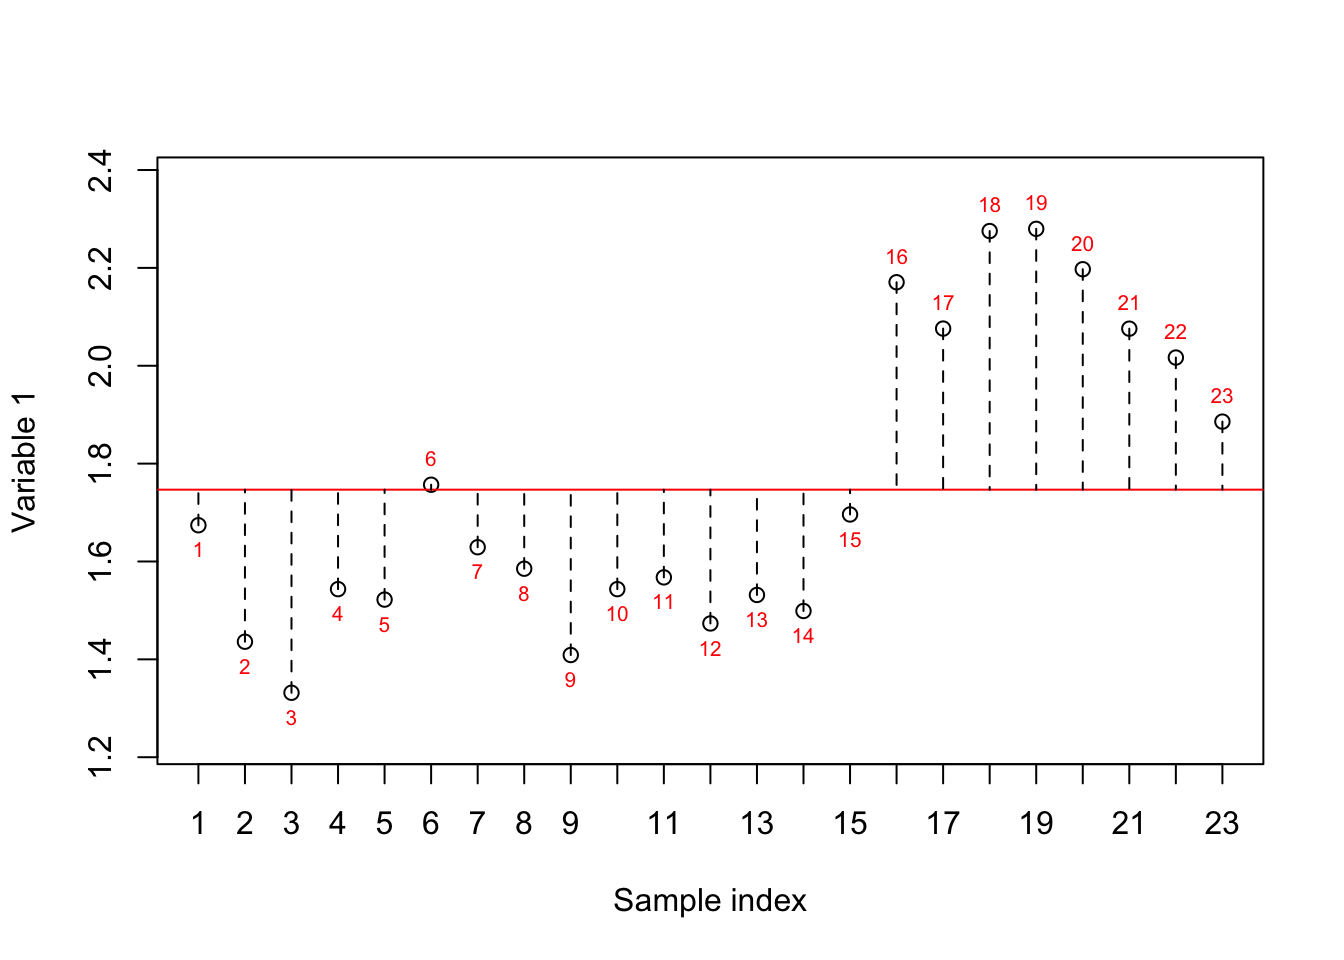
\includegraphics{PCA_files/figure-latex/fig-simple-variation-1} 

}

\caption{Here, we select one variable (a gene) and show how the data is spread around the mean. The red numbers show the index of each sample. The red line shows the mean and the dashed lines show the distance between each observation and mean}\label{fig:fig-simple-variation}
\end{figure}

In Figure \ref{fig:fig-simple-variation}, we have plotted the sample number (just a simple index) on the x axis and the expression of variable 1 on the y axis. The red line shows the mean (average) of the variable one and the dashed lines show the distance between each observation (sample) to the mean. The variation is simply the average of squared of these distances to the mean. However, we are still not sure whether the variation we are seen is of any interest for us. Let's reorder the samples based on the expression.

\begin{Shaded}
\begin{Highlighting}[]
\CommentTok{# Select variable}
\NormalTok{variableIndex<-}\DecValTok{18924}

\CommentTok{# plot the data for variable 1}
\CommentTok{# create x axis}
\NormalTok{x_axis<-}\KeywordTok{factor}\NormalTok{(}\KeywordTok{order}\NormalTok{(data[,variableIndex]),}\DataTypeTok{levels =} \KeywordTok{order}\NormalTok{(data[,variableIndex]))}
\KeywordTok{plot.default}\NormalTok{(}\DataTypeTok{x=}\NormalTok{x_axis,}
     \DataTypeTok{y=}\NormalTok{(}\KeywordTok{sort}\NormalTok{(data[,variableIndex])),}\DataTypeTok{xlab =} \StringTok{"Sample index"}\NormalTok{,}\DataTypeTok{ylab =} \KeywordTok{paste}\NormalTok{(}\StringTok{"Variable"}\NormalTok{,variableIndex),}
     \DataTypeTok{ylim =} \KeywordTok{c}\NormalTok{(}\KeywordTok{min}\NormalTok{(data[,variableIndex])}\OperatorTok{-}\FloatTok{0.1}\NormalTok{,}\KeywordTok{max}\NormalTok{(data[,variableIndex])}\OperatorTok{+}\FloatTok{0.1}\NormalTok{),}\DataTypeTok{xaxt=}\StringTok{'n'}\NormalTok{,}\DataTypeTok{col=}\KeywordTok{factor}\NormalTok{(metadata}\OperatorTok{$}\NormalTok{Covariate)[}\KeywordTok{order}\NormalTok{(data[,variableIndex])])}
\CommentTok{# add x axis}
\KeywordTok{axis}\NormalTok{(}\DataTypeTok{side =} \DecValTok{1}\NormalTok{, }\DataTypeTok{at =} \DecValTok{1}\OperatorTok{:}\KeywordTok{nrow}\NormalTok{(data), }\DataTypeTok{labels =}\NormalTok{ x_axis)}
\KeywordTok{legend}\NormalTok{(}\StringTok{"topleft"}\NormalTok{, }\DataTypeTok{legend=}\KeywordTok{c}\NormalTok{(}\KeywordTok{unique}\NormalTok{(}\KeywordTok{levels}\NormalTok{(}\KeywordTok{factor}\NormalTok{(metadata}\OperatorTok{$}\NormalTok{Covariate)))),}
       \DataTypeTok{col=}\KeywordTok{unique}\NormalTok{(}\KeywordTok{as.numeric}\NormalTok{(}\KeywordTok{factor}\NormalTok{(metadata}\OperatorTok{$}\NormalTok{Covariate))), }\DataTypeTok{cex=}\FloatTok{0.8}\NormalTok{, }\DataTypeTok{pch =} \DecValTok{1}\NormalTok{)}
\CommentTok{# fig position of labels}
\NormalTok{pos_plot<-(}\KeywordTok{as.numeric}\NormalTok{(}\KeywordTok{sort}\NormalTok{(data[,variableIndex])}\OperatorTok{>}\KeywordTok{mean}\NormalTok{(data[,variableIndex]))}\OperatorTok{*}\DecValTok{2}\NormalTok{)}\OperatorTok{+}\DecValTok{1}
\CommentTok{# Draw sample index}
\KeywordTok{text}\NormalTok{(}\DecValTok{1}\OperatorTok{:}\KeywordTok{nrow}\NormalTok{(data), }\KeywordTok{sort}\NormalTok{(data[,variableIndex]),  x_axis,}
     \DataTypeTok{cex=}\FloatTok{0.65}\NormalTok{,}\DataTypeTok{col=}\KeywordTok{as.numeric}\NormalTok{(}\KeywordTok{factor}\NormalTok{(metadata}\OperatorTok{$}\NormalTok{Covariate)[}\KeywordTok{order}\NormalTok{(data[,variableIndex])]),}\DataTypeTok{pos=}\NormalTok{pos_plot)}

\CommentTok{# draw the mean line}
\KeywordTok{abline}\NormalTok{(}\DataTypeTok{h=}\KeywordTok{mean}\NormalTok{(data[,variableIndex],),}\DataTypeTok{col=}\StringTok{"red"}\NormalTok{)}

\CommentTok{# for each observation draw a line from that point to the mean}
\ControlFlowTok{for}\NormalTok{(i }\ControlFlowTok{in} \DecValTok{1}\OperatorTok{:}\KeywordTok{nrow}\NormalTok{(data))}
\NormalTok{\{}
  \KeywordTok{segments}\NormalTok{(}\DataTypeTok{x0 =}\NormalTok{ i,}\DataTypeTok{x1 =}\NormalTok{ i,}\DataTypeTok{y0 =} \KeywordTok{sort}\NormalTok{(data[,variableIndex])[i],}\DataTypeTok{y1 =} \KeywordTok{mean}\NormalTok{(data[,variableIndex]),}\DataTypeTok{lty=}\StringTok{"dashed"}\NormalTok{,}\DataTypeTok{col=}
             \KeywordTok{factor}\NormalTok{(metadata}\OperatorTok{$}\NormalTok{Covariate)[}\KeywordTok{order}\NormalTok{(data[,variableIndex])][i])}
\NormalTok{\}}
\end{Highlighting}
\end{Shaded}

\begin{figure}

{\centering 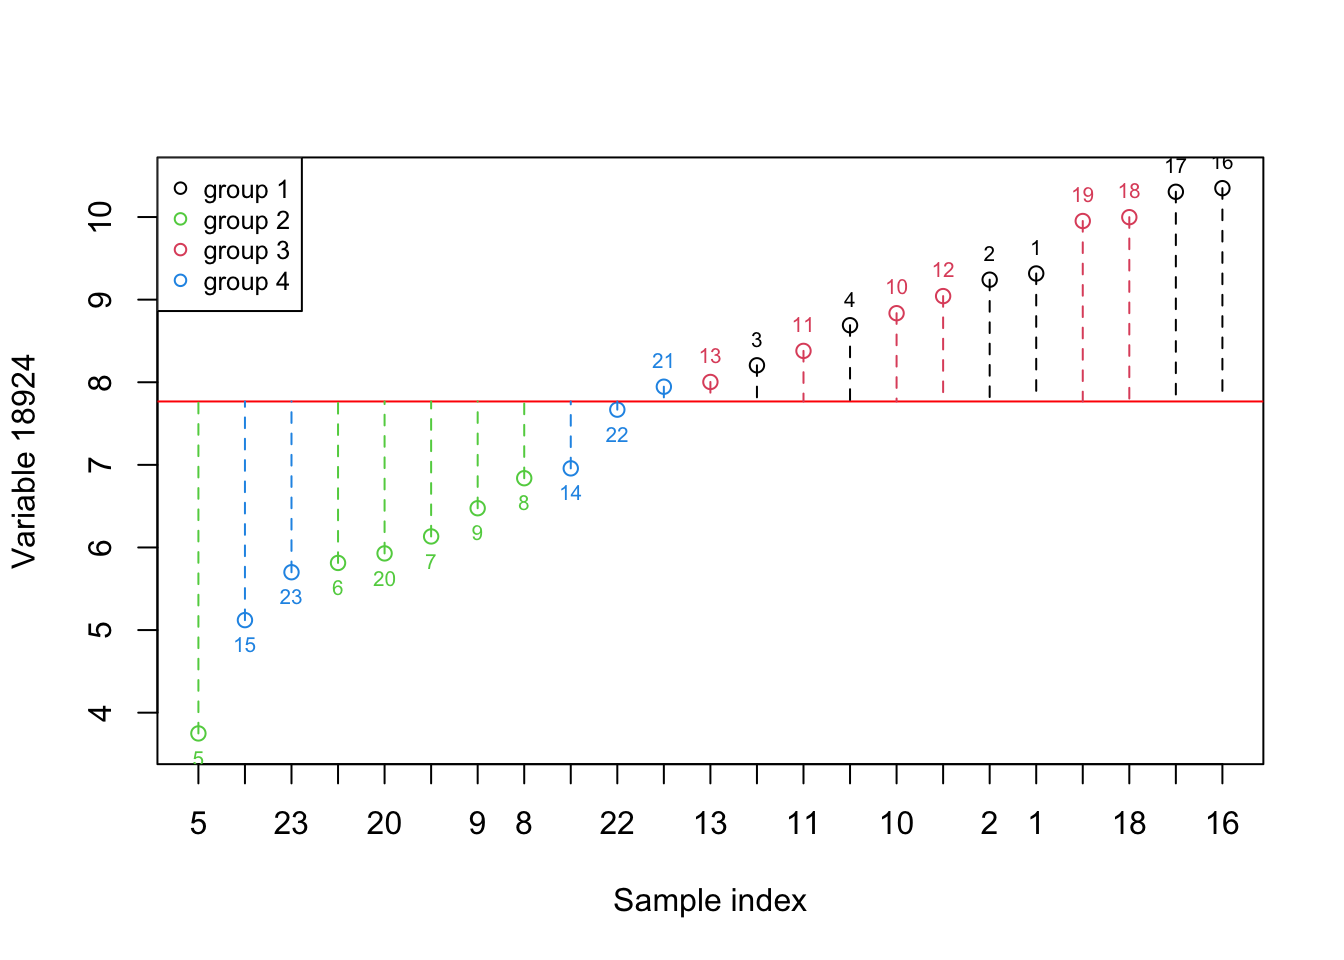
\includegraphics{PCA_files/figure-latex/fig-simple-variation-reorder-1} 

}

\caption{Here, we select one variable (a gene) and show how the data is spread around the mean. The red numbers show the index of each sample. The red line shows the mean and the dashed lines show the distance between each observation and mean. Please note that the samples are reordered based on expression. the color of points show the grouping of samples}\label{fig:fig-simple-variation-reorder}
\end{figure}

Figure \ref{fig:fig-simple-variation} shows the same variable as Figure \ref{fig:fig-simple-variation-reorder} but we have reorder the observations so that the ones with lower expression come first. We have also added color so that we can see where there is a difference between the groups in this experiment. What is clear now is that, the variation in this variable alone does not provide us with much useful information about all the groups. However, the second group appears to have lower expression compared to the rest of the groups. In addition, The First and the third group show higher expression compared to the rest.

That's great Let's pick another variable and plot the same thing:

\begin{Shaded}
\begin{Highlighting}[]
\CommentTok{# Select variable}
\NormalTok{variableIndex<-}\DecValTok{20355}

\CommentTok{# plot the data for variable 2}
\CommentTok{# create x axis}
\NormalTok{x_axis<-}\KeywordTok{factor}\NormalTok{(}\KeywordTok{order}\NormalTok{(data[,variableIndex]),}\DataTypeTok{levels =} \KeywordTok{order}\NormalTok{(data[,variableIndex]))}
\KeywordTok{plot.default}\NormalTok{(}\DataTypeTok{x=}\NormalTok{x_axis,}
     \DataTypeTok{y=}\NormalTok{(}\KeywordTok{sort}\NormalTok{(data[,variableIndex])),}\DataTypeTok{xlab =} \StringTok{"Sample index"}\NormalTok{,}\DataTypeTok{ylab =} \KeywordTok{paste}\NormalTok{(}\StringTok{"Variable"}\NormalTok{,variableIndex),}
     \DataTypeTok{ylim =} \KeywordTok{c}\NormalTok{(}\KeywordTok{min}\NormalTok{(data[,variableIndex])}\OperatorTok{-}\FloatTok{0.1}\NormalTok{,}\KeywordTok{max}\NormalTok{(data[,variableIndex])}\OperatorTok{+}\FloatTok{0.1}\NormalTok{),}\DataTypeTok{xaxt=}\StringTok{'n'}\NormalTok{,}\DataTypeTok{col=}\KeywordTok{factor}\NormalTok{(metadata}\OperatorTok{$}\NormalTok{Covariate)[}\KeywordTok{order}\NormalTok{(data[,variableIndex])])}
\CommentTok{# add x axis}
\KeywordTok{axis}\NormalTok{(}\DataTypeTok{side =} \DecValTok{1}\NormalTok{, }\DataTypeTok{at =} \DecValTok{1}\OperatorTok{:}\KeywordTok{nrow}\NormalTok{(data), }\DataTypeTok{labels =}\NormalTok{ x_axis)}
\KeywordTok{legend}\NormalTok{(}\StringTok{"topleft"}\NormalTok{, }\DataTypeTok{legend=}\KeywordTok{c}\NormalTok{(}\KeywordTok{unique}\NormalTok{(}\KeywordTok{levels}\NormalTok{(}\KeywordTok{factor}\NormalTok{(metadata}\OperatorTok{$}\NormalTok{Covariate)))),}
       \DataTypeTok{col=}\KeywordTok{unique}\NormalTok{(}\KeywordTok{as.numeric}\NormalTok{(}\KeywordTok{factor}\NormalTok{(metadata}\OperatorTok{$}\NormalTok{Covariate))), }\DataTypeTok{cex=}\FloatTok{0.8}\NormalTok{, }\DataTypeTok{pch =} \DecValTok{1}\NormalTok{)}
\CommentTok{# fig position of labels}
\NormalTok{pos_plot<-(}\KeywordTok{as.numeric}\NormalTok{(}\KeywordTok{sort}\NormalTok{(data[,variableIndex])}\OperatorTok{>}\KeywordTok{mean}\NormalTok{(data[,variableIndex]))}\OperatorTok{*}\DecValTok{2}\NormalTok{)}\OperatorTok{+}\DecValTok{1}
\CommentTok{# Draw sample index}
\KeywordTok{text}\NormalTok{(}\DecValTok{1}\OperatorTok{:}\KeywordTok{nrow}\NormalTok{(data), }\KeywordTok{sort}\NormalTok{(data[,variableIndex]),  x_axis,}
     \DataTypeTok{cex=}\FloatTok{0.65}\NormalTok{,}\DataTypeTok{col=}\KeywordTok{as.numeric}\NormalTok{(}\KeywordTok{factor}\NormalTok{(metadata}\OperatorTok{$}\NormalTok{Covariate)[}\KeywordTok{order}\NormalTok{(data[,variableIndex])]),}\DataTypeTok{pos=}\NormalTok{pos_plot)}

\CommentTok{# draw the mean line}
\KeywordTok{abline}\NormalTok{(}\DataTypeTok{h=}\KeywordTok{mean}\NormalTok{(data[,variableIndex],),}\DataTypeTok{col=}\StringTok{"red"}\NormalTok{)}

\CommentTok{# for each observation draw a line from that point to the mean}
\ControlFlowTok{for}\NormalTok{(i }\ControlFlowTok{in} \DecValTok{1}\OperatorTok{:}\KeywordTok{nrow}\NormalTok{(data))}
\NormalTok{\{}
  \KeywordTok{segments}\NormalTok{(}\DataTypeTok{x0 =}\NormalTok{ i,}\DataTypeTok{x1 =}\NormalTok{ i,}\DataTypeTok{y0 =} \KeywordTok{sort}\NormalTok{(data[,variableIndex])[i],}\DataTypeTok{y1 =} \KeywordTok{mean}\NormalTok{(data[,variableIndex]),}\DataTypeTok{lty=}\StringTok{"dashed"}\NormalTok{,}\DataTypeTok{col=}
             \KeywordTok{factor}\NormalTok{(metadata}\OperatorTok{$}\NormalTok{Covariate)[}\KeywordTok{order}\NormalTok{(data[,variableIndex])][i])}
\NormalTok{\}}
\end{Highlighting}
\end{Shaded}

\begin{figure}

{\centering 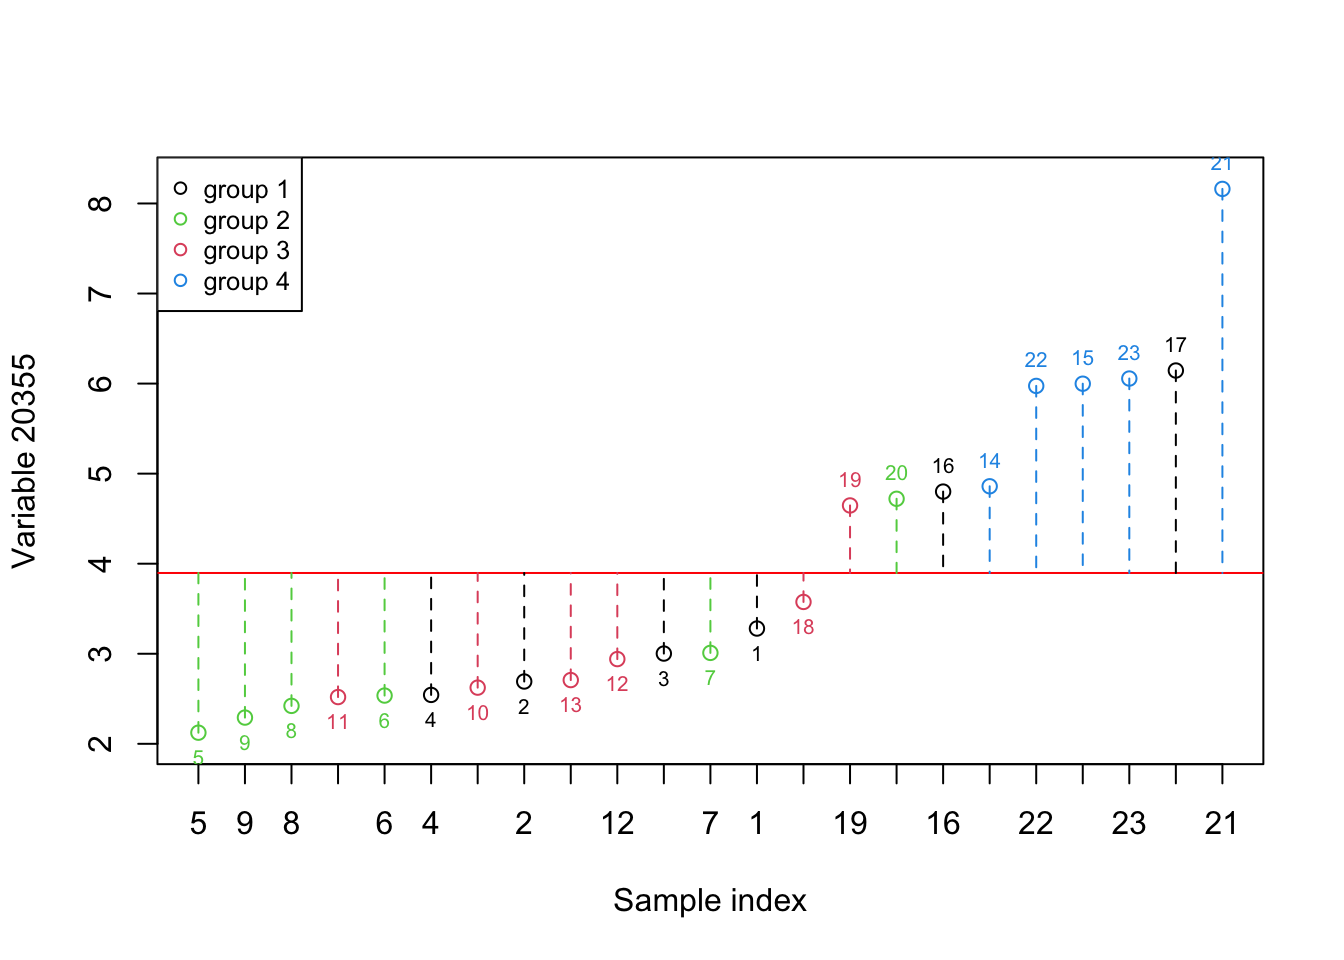
\includegraphics{PCA_files/figure-latex/fig-simple-variation-reorder-v2-1} 

}

\caption{Here, we select one variable (a gene) and show how the data is spread around the mean. The red numbers show the index of each sample. The red line shows the mean and the dashed lines show the distance between each observation and mean. Please note that the samples are reordered based on expression. the color of points show the grouping of samples}\label{fig:fig-simple-variation-reorder-v2}
\end{figure}

As it's evident in Figure \ref{fig:fig-simple-variation-reorder-v2}, the variation in this variable shows us the difference between the fourth group and the rest but it does not provide much information about the the rest of the groups. Let's have a look at what information both of these variable give. We simply put both figures Figure \ref{fig:fig-simple-variation-reorder} and Figure \ref{fig:fig-simple-variation-reorder-v2} together:

\begin{Shaded}
\begin{Highlighting}[]
\KeywordTok{par}\NormalTok{(}\DataTypeTok{mfrow=}\KeywordTok{c}\NormalTok{(}\DecValTok{2}\NormalTok{,}\DecValTok{1}\NormalTok{))}
\CommentTok{# Select variable}
\NormalTok{variableIndex<-}\DecValTok{18924}

\CommentTok{# plot the data for variable 1}
\CommentTok{# create x axis}
\NormalTok{x_axis<-}\KeywordTok{factor}\NormalTok{(}\KeywordTok{order}\NormalTok{(data[,variableIndex]),}\DataTypeTok{levels =} \KeywordTok{order}\NormalTok{(data[,variableIndex]))}
\KeywordTok{plot.default}\NormalTok{(}\DataTypeTok{x=}\NormalTok{x_axis,}
     \DataTypeTok{y=}\NormalTok{(}\KeywordTok{sort}\NormalTok{(data[,variableIndex])),}\DataTypeTok{xlab =} \StringTok{"Sample index"}\NormalTok{,}\DataTypeTok{ylab =} \KeywordTok{paste}\NormalTok{(}\StringTok{"Variable"}\NormalTok{,variableIndex),}
     \DataTypeTok{ylim =} \KeywordTok{c}\NormalTok{(}\KeywordTok{min}\NormalTok{(data[,variableIndex])}\OperatorTok{-}\FloatTok{0.1}\NormalTok{,}\KeywordTok{max}\NormalTok{(data[,variableIndex])}\OperatorTok{+}\FloatTok{0.1}\NormalTok{),}\DataTypeTok{xaxt=}\StringTok{'n'}\NormalTok{,}
     \DataTypeTok{col=}\KeywordTok{factor}\NormalTok{(metadata}\OperatorTok{$}\NormalTok{Covariate)[}\KeywordTok{order}\NormalTok{(data[,variableIndex])])}
\CommentTok{# add x axis}
\KeywordTok{axis}\NormalTok{(}\DataTypeTok{side =} \DecValTok{1}\NormalTok{, }\DataTypeTok{at =} \DecValTok{1}\OperatorTok{:}\KeywordTok{nrow}\NormalTok{(data), }\DataTypeTok{labels =}\NormalTok{ x_axis)}
\KeywordTok{legend}\NormalTok{(}\StringTok{"topleft"}\NormalTok{, }\DataTypeTok{legend=}\KeywordTok{c}\NormalTok{(}\KeywordTok{unique}\NormalTok{(}\KeywordTok{levels}\NormalTok{(}\KeywordTok{factor}\NormalTok{(metadata}\OperatorTok{$}\NormalTok{Covariate)))),}
       \DataTypeTok{col=}\KeywordTok{unique}\NormalTok{(}\KeywordTok{as.numeric}\NormalTok{(}\KeywordTok{factor}\NormalTok{(metadata}\OperatorTok{$}\NormalTok{Covariate))), }\DataTypeTok{cex=}\FloatTok{0.8}\NormalTok{, }\DataTypeTok{pch =} \DecValTok{1}\NormalTok{)}
\CommentTok{# fig position of labels}
\NormalTok{pos_plot<-(}\KeywordTok{as.numeric}\NormalTok{(}\KeywordTok{sort}\NormalTok{(data[,variableIndex])}\OperatorTok{>}\KeywordTok{mean}\NormalTok{(data[,variableIndex]))}\OperatorTok{*}\DecValTok{2}\NormalTok{)}\OperatorTok{+}\DecValTok{1}
\CommentTok{# Draw sample index}
\KeywordTok{text}\NormalTok{(}\DecValTok{1}\OperatorTok{:}\KeywordTok{nrow}\NormalTok{(data), }\KeywordTok{sort}\NormalTok{(data[,variableIndex]),  x_axis,}
     \DataTypeTok{cex=}\FloatTok{0.65}\NormalTok{,}\DataTypeTok{col=}\KeywordTok{as.numeric}\NormalTok{(}\KeywordTok{factor}\NormalTok{(metadata}\OperatorTok{$}\NormalTok{Covariate)[}\KeywordTok{order}\NormalTok{(data[,variableIndex])]),}\DataTypeTok{pos=}\NormalTok{pos_plot)}

\CommentTok{# draw the mean line}
\KeywordTok{abline}\NormalTok{(}\DataTypeTok{h=}\KeywordTok{mean}\NormalTok{(data[,variableIndex],),}\DataTypeTok{col=}\StringTok{"red"}\NormalTok{)}

\CommentTok{# for each observation draw a line from that point to the mean}
\ControlFlowTok{for}\NormalTok{(i }\ControlFlowTok{in} \DecValTok{1}\OperatorTok{:}\KeywordTok{nrow}\NormalTok{(data))}
\NormalTok{\{}
  \KeywordTok{segments}\NormalTok{(}\DataTypeTok{x0 =}\NormalTok{ i,}\DataTypeTok{x1 =}\NormalTok{ i,}\DataTypeTok{y0 =} \KeywordTok{sort}\NormalTok{(data[,variableIndex])[i],}\DataTypeTok{y1 =} \KeywordTok{mean}\NormalTok{(data[,variableIndex]),}\DataTypeTok{lty=}\StringTok{"dashed"}\NormalTok{,}\DataTypeTok{col=}
             \KeywordTok{factor}\NormalTok{(metadata}\OperatorTok{$}\NormalTok{Covariate)[}\KeywordTok{order}\NormalTok{(data[,variableIndex])][i])}
\NormalTok{\}}

\CommentTok{# Select variable}
\NormalTok{variableIndex<-}\DecValTok{20355}

\CommentTok{# plot the data for variable 2}
\CommentTok{# create x axis}
\NormalTok{x_axis<-}\KeywordTok{factor}\NormalTok{(}\KeywordTok{order}\NormalTok{(data[,variableIndex]),}\DataTypeTok{levels =} \KeywordTok{order}\NormalTok{(data[,variableIndex]))}
\KeywordTok{plot.default}\NormalTok{(}\DataTypeTok{x=}\NormalTok{x_axis,}
     \DataTypeTok{y=}\NormalTok{(}\KeywordTok{sort}\NormalTok{(data[,variableIndex])),}\DataTypeTok{xlab =} \StringTok{"Sample index"}\NormalTok{,}\DataTypeTok{ylab =} \KeywordTok{paste}\NormalTok{(}\StringTok{"Variable"}\NormalTok{,variableIndex),}
     \DataTypeTok{ylim =} \KeywordTok{c}\NormalTok{(}\KeywordTok{min}\NormalTok{(data[,variableIndex])}\OperatorTok{-}\FloatTok{0.1}\NormalTok{,}\KeywordTok{max}\NormalTok{(data[,variableIndex])}\OperatorTok{+}\FloatTok{0.1}\NormalTok{),}\DataTypeTok{xaxt=}\StringTok{'n'}\NormalTok{,}
     \DataTypeTok{col=}\KeywordTok{factor}\NormalTok{(metadata}\OperatorTok{$}\NormalTok{Covariate)[}\KeywordTok{order}\NormalTok{(data[,variableIndex])])}
\CommentTok{# add x axis}
\KeywordTok{axis}\NormalTok{(}\DataTypeTok{side =} \DecValTok{1}\NormalTok{, }\DataTypeTok{at =} \DecValTok{1}\OperatorTok{:}\KeywordTok{nrow}\NormalTok{(data), }\DataTypeTok{labels =}\NormalTok{ x_axis)}
\KeywordTok{legend}\NormalTok{(}\StringTok{"topleft"}\NormalTok{, }\DataTypeTok{legend=}\KeywordTok{c}\NormalTok{(}\KeywordTok{unique}\NormalTok{(}\KeywordTok{levels}\NormalTok{(}\KeywordTok{factor}\NormalTok{(metadata}\OperatorTok{$}\NormalTok{Covariate)))),}
       \DataTypeTok{col=}\KeywordTok{unique}\NormalTok{(}\KeywordTok{as.numeric}\NormalTok{(}\KeywordTok{factor}\NormalTok{(metadata}\OperatorTok{$}\NormalTok{Covariate))), }\DataTypeTok{cex=}\FloatTok{0.8}\NormalTok{, }\DataTypeTok{pch =} \DecValTok{1}\NormalTok{)}
\CommentTok{# fig position of labels}
\NormalTok{pos_plot<-(}\KeywordTok{as.numeric}\NormalTok{(}\KeywordTok{sort}\NormalTok{(data[,variableIndex])}\OperatorTok{>}\KeywordTok{mean}\NormalTok{(data[,variableIndex]))}\OperatorTok{*}\DecValTok{2}\NormalTok{)}\OperatorTok{+}\DecValTok{1}
\CommentTok{# Draw sample index}
\KeywordTok{text}\NormalTok{(}\DecValTok{1}\OperatorTok{:}\KeywordTok{nrow}\NormalTok{(data), }\KeywordTok{sort}\NormalTok{(data[,variableIndex]),  x_axis,}
     \DataTypeTok{cex=}\FloatTok{0.65}\NormalTok{,}\DataTypeTok{col=}\KeywordTok{as.numeric}\NormalTok{(}\KeywordTok{factor}\NormalTok{(metadata}\OperatorTok{$}\NormalTok{Covariate)[}\KeywordTok{order}\NormalTok{(data[,variableIndex])]),}\DataTypeTok{pos=}\NormalTok{pos_plot)}

\CommentTok{# draw the mean line}
\KeywordTok{abline}\NormalTok{(}\DataTypeTok{h=}\KeywordTok{mean}\NormalTok{(data[,variableIndex],),}\DataTypeTok{col=}\StringTok{"red"}\NormalTok{)}

\CommentTok{# for each observation draw a line from that point to the mean}
\ControlFlowTok{for}\NormalTok{(i }\ControlFlowTok{in} \DecValTok{1}\OperatorTok{:}\KeywordTok{nrow}\NormalTok{(data))}
\NormalTok{\{}
  \KeywordTok{segments}\NormalTok{(}\DataTypeTok{x0 =}\NormalTok{ i,}\DataTypeTok{x1 =}\NormalTok{ i,}\DataTypeTok{y0 =} \KeywordTok{sort}\NormalTok{(data[,variableIndex])[i],}\DataTypeTok{y1 =} \KeywordTok{mean}\NormalTok{(data[,variableIndex]),}\DataTypeTok{lty=}\StringTok{"dashed"}\NormalTok{,}\DataTypeTok{col=}
             \KeywordTok{factor}\NormalTok{(metadata}\OperatorTok{$}\NormalTok{Covariate)[}\KeywordTok{order}\NormalTok{(data[,variableIndex])][i])}
\NormalTok{\}}
\end{Highlighting}
\end{Shaded}

\begin{figure}

{\centering 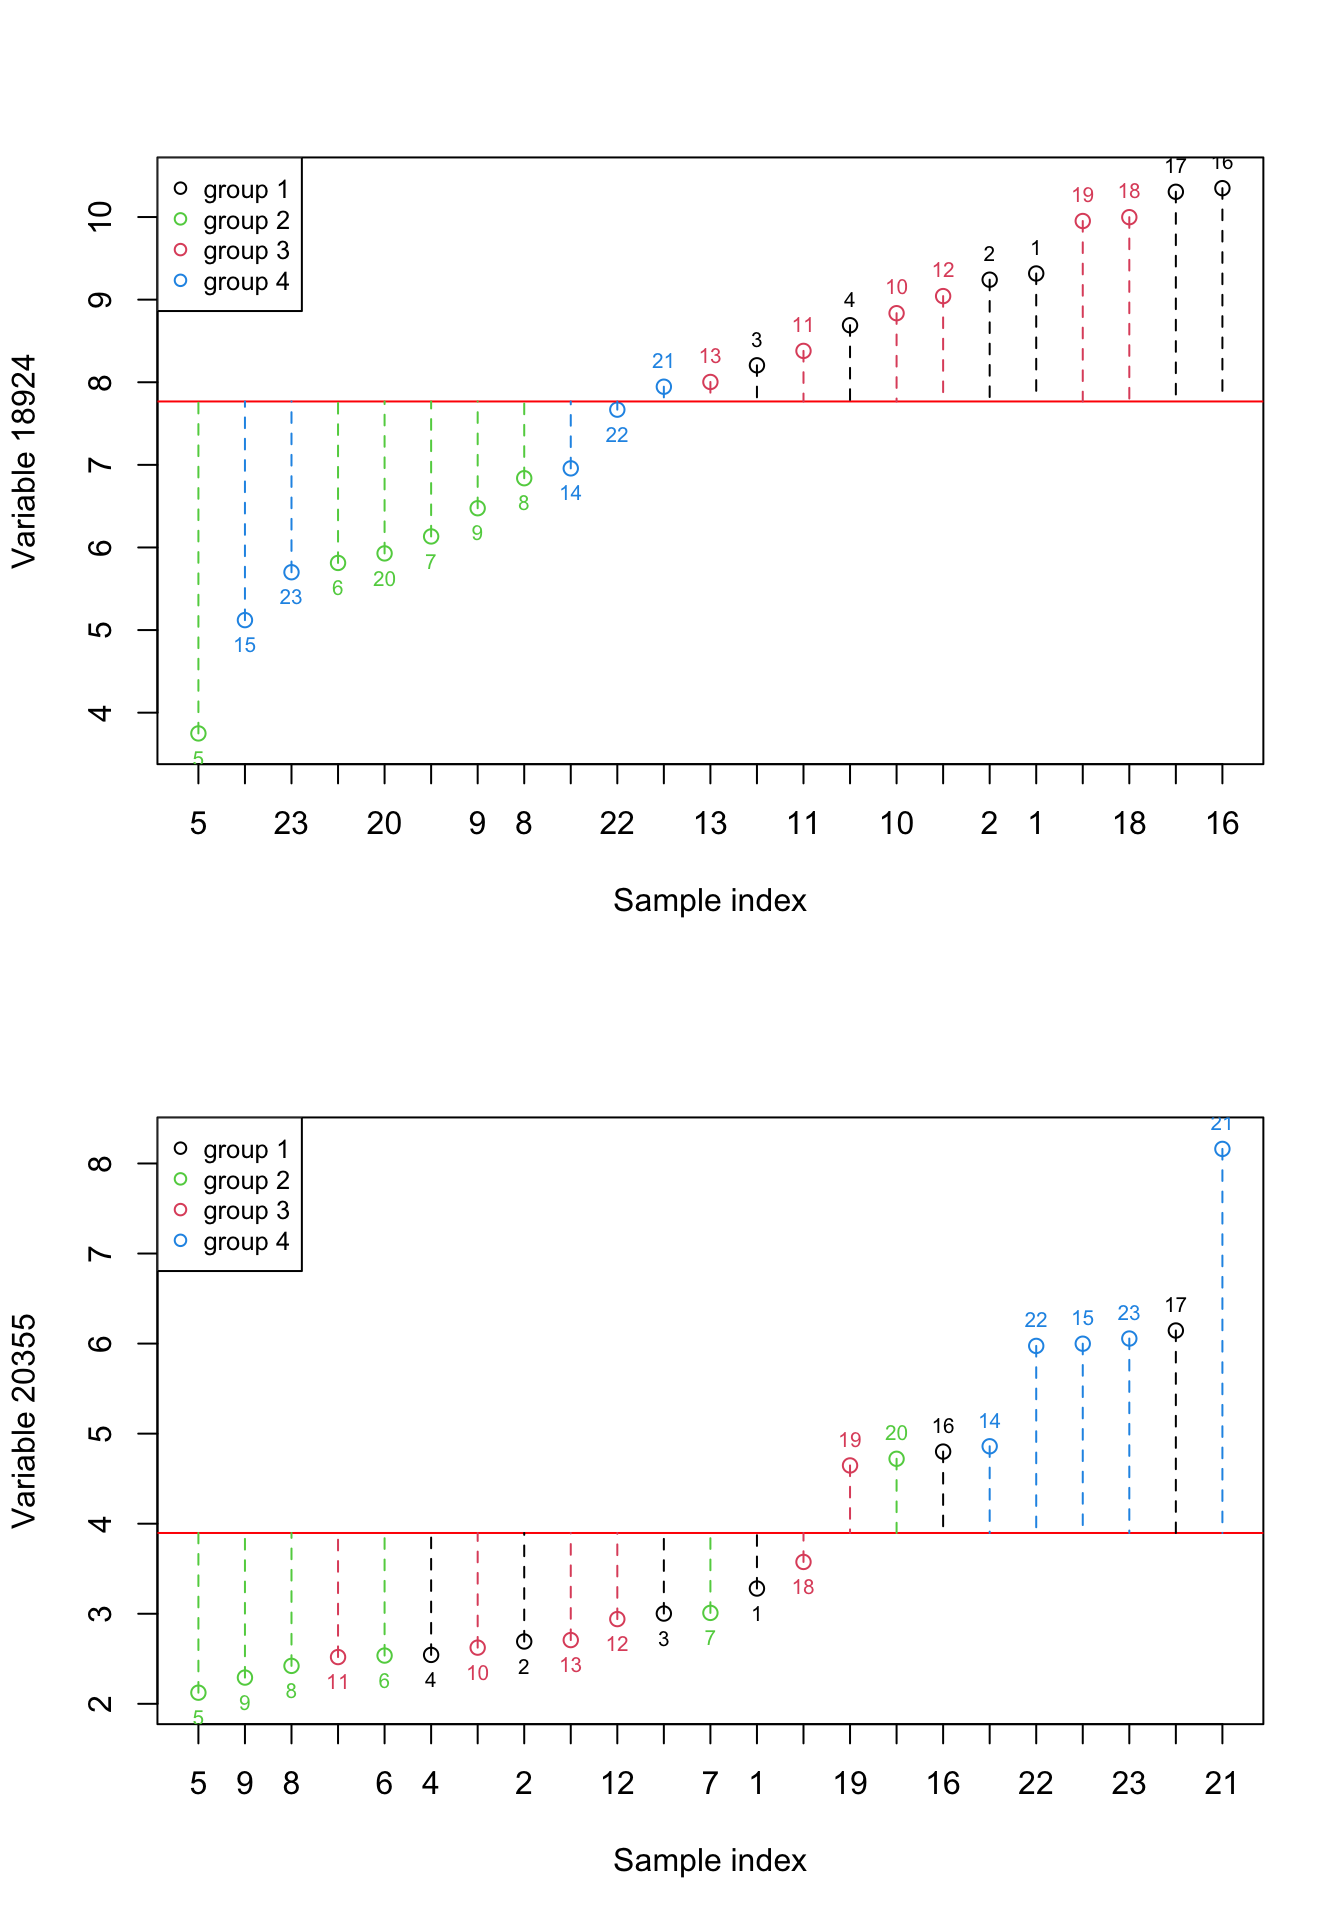
\includegraphics{PCA_files/figure-latex/fig-simple-variation-reorder-v3-1} 

}

\caption{Here, we select two previous variables and show how the data is spread around the mean. The red numbers show the index of each sample. The red line shows the mean and the dashed lines show the distance between each observation and mean. Please note that the samples are reordered based on expression. the color of points show the grouping of samples}\label{fig:fig-simple-variation-reorder-v3}
\end{figure}

We can see in Figure \ref{fig:fig-simple-variation-reorder-v3}, there is obviously some information that is almost only explained by individual variables. For example the differences between group 2 and group 4 is mostly explained by variable 20355. But there is also some small information that seems to be redundant. For example the differences between combined groups 1 and 3 vs group 4. We can have a look at variation and redundancy together by plotting the expressions of both variables against each other.

plot(data{[},c(18924,20355){]},col=factor(metadata\$Covariate))

\begin{Shaded}
\begin{Highlighting}[]
\CommentTok{# define variables}
\NormalTok{var1<-}\DecValTok{18924}
\NormalTok{var2<-}\DecValTok{20355}
\CommentTok{# plot the data}
\KeywordTok{plot}\NormalTok{(data[,}\KeywordTok{c}\NormalTok{(var1,var2)],}\DataTypeTok{col=}\KeywordTok{factor}\NormalTok{(metadata}\OperatorTok{$}\NormalTok{Covariate),}\DataTypeTok{xlab =} \StringTok{"Variable 1"}\NormalTok{, }\DataTypeTok{ylab =} \StringTok{"Variable 2"}\NormalTok{)}
\CommentTok{# create legend}
\KeywordTok{legend}\NormalTok{(}\StringTok{"topleft"}\NormalTok{, }\DataTypeTok{legend=}\KeywordTok{c}\NormalTok{(}\KeywordTok{unique}\NormalTok{(}\KeywordTok{levels}\NormalTok{(}\KeywordTok{factor}\NormalTok{(metadata}\OperatorTok{$}\NormalTok{Covariate)))),}
       \DataTypeTok{col=}\KeywordTok{unique}\NormalTok{(}\KeywordTok{as.numeric}\NormalTok{(}\KeywordTok{factor}\NormalTok{(metadata}\OperatorTok{$}\NormalTok{Covariate))), }\DataTypeTok{cex=}\FloatTok{0.8}\NormalTok{, }\DataTypeTok{pch =} \DecValTok{1}\NormalTok{)}
\CommentTok{# fig position of labels}
\NormalTok{pos_plot<-(}\KeywordTok{as.numeric}\NormalTok{(}\KeywordTok{sort}\NormalTok{(data[,variableIndex])}\OperatorTok{>}\KeywordTok{mean}\NormalTok{(data[,variableIndex]))}\OperatorTok{*}\DecValTok{2}\NormalTok{)}\OperatorTok{+}\DecValTok{1}
\CommentTok{# Draw sample index}
\KeywordTok{text}\NormalTok{((data[,var1]), (data[,var2]),  }\DecValTok{1}\OperatorTok{:}\KeywordTok{nrow}\NormalTok{(data),}
     \DataTypeTok{cex=}\FloatTok{0.65}\NormalTok{,}\DataTypeTok{col=}\KeywordTok{as.numeric}\NormalTok{(}\KeywordTok{factor}\NormalTok{(metadata}\OperatorTok{$}\NormalTok{Covariate)),}\DataTypeTok{pos=}\NormalTok{pos_plot)}
\end{Highlighting}
\end{Shaded}

\begin{figure}

{\centering 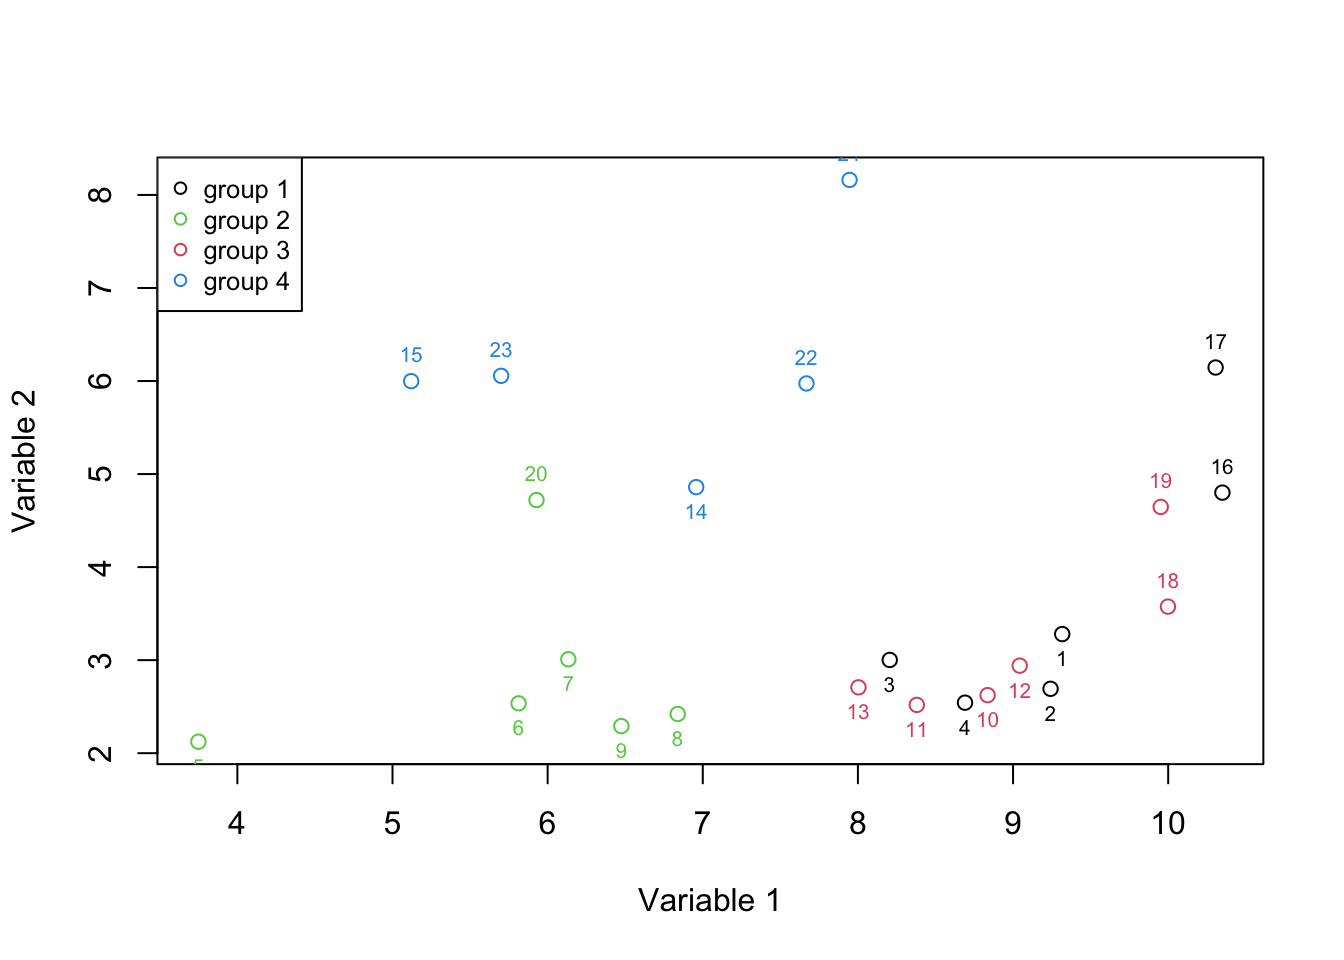
\includegraphics{PCA_files/figure-latex/fig-simple-cov-1} 

}

\caption{Here, we select two variables and show how the data is spread according to both of the variables.}\label{fig:fig-simple-cov}
\end{figure}

Figure \ref{fig:fig-simple-cov} is called 2d scatter plot that is used to show the relationships between two variables. It's now more evident that we can separate group 2 and 4 more easily. This means the combination of two variables gave us more information than a single variable at the time. At this time we can more formally say that we have two axis x and y (Variable 1 and 2) which define our data. Each axis has some information. To quantify that information, let's agree that the amount of information in each axis is measured by variation of the observations in that axis.
As said before, the variation is define as the the average squared distances from the mean. That can be easily computer using a simple R function (var):

\begin{Shaded}
\begin{Highlighting}[]
\CommentTok{# calculate variation of variable 1}
\NormalTok{variation_var1<-}\KeywordTok{var}\NormalTok{(data[,var1])}

\CommentTok{# calculate variation of variable 2}
\NormalTok{variation_var2<-}\KeywordTok{var}\NormalTok{(data[,var2])}

\KeywordTok{sprintf}\NormalTok{(}\StringTok{"Variation of variable1: %f Varition of variable2: %f"}\NormalTok{,variation_var1,variation_var2)}
\end{Highlighting}
\end{Shaded}

\begin{verbatim}
## [1] "Variation of variable1: 3.282278 Varition of variable2: 2.753621"
\end{verbatim}

In the beginning it might sound to use variation to quantify information as one variable can contain huge noise level that can easily be higher than another variable that is more informative. However, in the presence of no addition information (such as groups in this example), we can at least assume (hope) that if the experiment has been done perfectly the variation of information is higher than variation of noise. So in this case, we can say that variable 1 has more information than variable 2.

We also mentioned that any two variables can possibly contain redundant information. To quantify that, we use a method that is called covariance. Covariance measures to what extend two variables are showing the same information. To calculate the covariance, for each of the observations (samples), we calculate difference of that observation to the mean for variable 1, we do the same thing for variable 2 and then multiply this the resulting numbers number. Once we did that for all the observations, we sum all the numbers and divide the results by total number of observations. The sign of covariance tells whether the two variables are positively or negatively related. The magnitude of covariance can be thought as total variation or the amount of redundancy between two samples. The higher the absolute value the higher the redundancy (we go through this in detail in the next chapters). The covariance of zero or close to zero means we have no or little redundancy.

Let's try to see what's visually happening:

\begin{Shaded}
\begin{Highlighting}[]
\CommentTok{# define variables}
\NormalTok{var1<-}\DecValTok{18924}
\NormalTok{var2<-}\DecValTok{20355}
\CommentTok{# plot the data}
\KeywordTok{plot}\NormalTok{(data[,}\KeywordTok{c}\NormalTok{(var1,var2)],}\DataTypeTok{xlab =} \StringTok{"Variable 1"}\NormalTok{, }\DataTypeTok{ylab =} \StringTok{"Variable 2"}\NormalTok{)}

\CommentTok{# fig position of labels}
\NormalTok{pos_plot<-(}\KeywordTok{as.numeric}\NormalTok{(}\KeywordTok{sort}\NormalTok{(data[,variableIndex])}\OperatorTok{>}\KeywordTok{mean}\NormalTok{(data[,variableIndex]))}\OperatorTok{*}\DecValTok{2}\NormalTok{)}\OperatorTok{+}\DecValTok{1}
\CommentTok{# Draw sample index}
\KeywordTok{text}\NormalTok{((data[,var1]), (data[,var2]),  }\DecValTok{1}\OperatorTok{:}\KeywordTok{nrow}\NormalTok{(data),}
     \DataTypeTok{cex=}\FloatTok{0.65}\NormalTok{,}\DataTypeTok{pos=}\NormalTok{pos_plot)}

\CommentTok{# plot mean of variable 1}
\KeywordTok{abline}\NormalTok{(}\DataTypeTok{v=}\KeywordTok{mean}\NormalTok{(data[,var1]),}\DataTypeTok{col=}\StringTok{"purple"}\NormalTok{,}\DataTypeTok{lty=}\DecValTok{1}\NormalTok{)}

\CommentTok{# plot mean of variable 2}
\KeywordTok{abline}\NormalTok{(}\DataTypeTok{h=}\KeywordTok{mean}\NormalTok{(data[,var2]),}\DataTypeTok{col=}\StringTok{"coral"}\NormalTok{,}\DataTypeTok{lty=}\DecValTok{1}\NormalTok{)}

\ControlFlowTok{for}\NormalTok{(i }\ControlFlowTok{in} \DecValTok{1}\OperatorTok{:}\KeywordTok{nrow}\NormalTok{(data))}
\NormalTok{\{}
  
    \KeywordTok{segments}\NormalTok{(}\DataTypeTok{x0 =}\NormalTok{ (data[,var1])[i],}\DataTypeTok{x1 =} \KeywordTok{mean}\NormalTok{(data[,var1]),}\DataTypeTok{y0 =}\NormalTok{ (data[,var2])[i],}\DataTypeTok{y1 =}\NormalTok{  (data[,var2])[i],}\DataTypeTok{lty=}\StringTok{"dashed"}\NormalTok{,}
             \DataTypeTok{col=}\KeywordTok{ifelse}\NormalTok{(data[i,var1]}\OperatorTok{>}\KeywordTok{mean}\NormalTok{(data[,var1]),}\DataTypeTok{yes =} \StringTok{"indianred1"}\NormalTok{,}\DataTypeTok{no =} \StringTok{"lightblue"}\NormalTok{))}
  
  
    \KeywordTok{segments}\NormalTok{(}\DataTypeTok{x0 =}\NormalTok{ (data[,var1])[i],}\DataTypeTok{x1 =}\NormalTok{ (data[,var1])[i],}\DataTypeTok{y0 =}\NormalTok{ (data[,var2])[i],}\DataTypeTok{y1 =}  \KeywordTok{mean}\NormalTok{(data[,var2]),}\DataTypeTok{lty=}\StringTok{"dashed"}\NormalTok{,}
             \DataTypeTok{col=}\KeywordTok{ifelse}\NormalTok{(data[i,var2]}\OperatorTok{>}\KeywordTok{mean}\NormalTok{(data[,var2]),}\DataTypeTok{yes =} \StringTok{"indianred1"}\NormalTok{,}\DataTypeTok{no =} \StringTok{"lightblue"}\NormalTok{))}
\NormalTok{\}}

\CommentTok{# add areas to the plot}

\KeywordTok{text}\NormalTok{(}\DecValTok{4}\NormalTok{,}\DecValTok{8}\NormalTok{,}\StringTok{"Area 1"}\NormalTok{)}
\KeywordTok{text}\NormalTok{(}\DecValTok{10}\NormalTok{,}\DecValTok{8}\NormalTok{,}\StringTok{"Area 2"}\NormalTok{)}
\KeywordTok{text}\NormalTok{(}\DecValTok{10}\NormalTok{,}\FloatTok{2.5}\NormalTok{,}\StringTok{"Area 3"}\NormalTok{)}
\KeywordTok{text}\NormalTok{(}\DecValTok{4}\NormalTok{,}\FloatTok{2.5}\NormalTok{,}\StringTok{"Area 4"}\NormalTok{)}
\end{Highlighting}
\end{Shaded}

\begin{figure}

{\centering 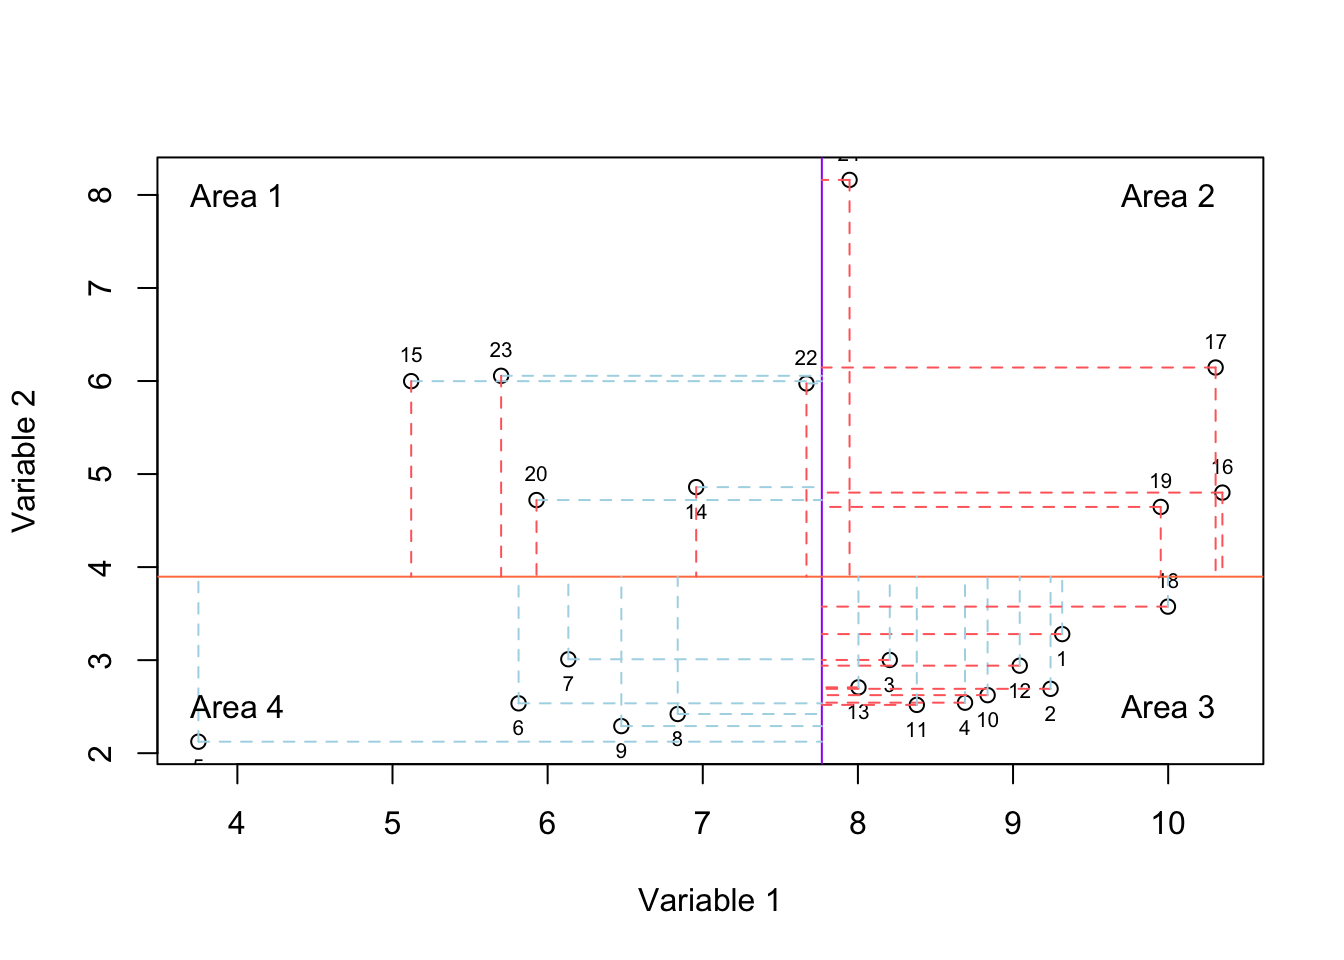
\includegraphics{PCA_files/figure-latex/fig-simple-cov2-1} 

}

\caption{Here, we select two variables and show how the data is spread according to both of the variables. The solid purple and coral lines show mean of variable and variable 2, respectively. For each observation, we have two lines showing whether it has higher or lower value compared to mean of variable one and variable 2.}\label{fig:fig-simple-cov2}
\end{figure}

In Figure \ref{fig:fig-simple-cov2}, we have plotted the mean of variable 1 using the vertical purple line and mean of the variable 2 using horizontal coral line. For each observation we have two lines, vertical line shows the difference of that observation to mean of variable 1 and horizontal line show the difference to the mean of variable 2. If the line is red, it means the difference is higher than zero and if the mean is blue, it means the difference is negative thus lower than zero.

If an observation lays in areas 1 or 3, it means that it behaves oppositely (relative to the mean: solid lines) in variable 1 and 2. This means if the expression goes up in variable 1, it goes down in variable 2 (or vice versa). However, if an observation lays in areas 2 or 4, it means its behavior is consistent in both of the variables. If most observation end of being in areas 2 and 4, we will have a positive covariance, meaning that they change consistently both in variable 1 and variable 2. If most of them are in area 1 and 3, we will have a negative covariance, meaning that they change in opposite directions. If the observations lay in all the four areas with approximately the same magnitude (distance to the mean: length of the red and blue lines), we will have a low or no covariance.

Please note that, the magnitude of the distances to the mean is also very important. For example even if all the observations end up in the areas 1 and 3 but one observation lays in area 2 with a very large distance from the means, we could still get a large positive covariance. In R the covariance is calculated using ``cov'' function:

\begin{Shaded}
\begin{Highlighting}[]
\CommentTok{# calculate variation of variable 1}
\NormalTok{covariation_var1_}\DecValTok{2}\NormalTok{<-}\KeywordTok{cov}\NormalTok{(data[,var1],data[,var2])}

\KeywordTok{sprintf}\NormalTok{(}\StringTok{"Covariation of variable1 and variable 2 is: %f"}\NormalTok{,covariation_var1_}\DecValTok{2}\NormalTok{)}
\end{Highlighting}
\end{Shaded}

\begin{verbatim}
## [1] "Covariation of variable1 and variable 2 is: 0.172791"
\end{verbatim}

We see that we got a low covariance which means that we have small redundancy in the two variables. This was expected just by looking at the Figure \ref{fig:fig-simple-cov2}. Most of our observations ended up being scattered in all four ares with very similar magnitudes.

This might be exiting as we have two variables that are showing complimentary information. We did not waste our resources on measuring the things that are showing the same information. However, we have bigger issue here! We just took a look at two of the variables out of 45101 measured ones! We specifically selected these variable to show this information. Look at this new variable:

\begin{Shaded}
\begin{Highlighting}[]
\CommentTok{# define number of plots in the figure}
\KeywordTok{par}\NormalTok{(}\DataTypeTok{mfrow=}\KeywordTok{c}\NormalTok{(}\DecValTok{1}\NormalTok{,}\DecValTok{3}\NormalTok{))}

\CommentTok{# define variables}
\NormalTok{var1<-}\DecValTok{18924}
\NormalTok{var2<-}\DecValTok{20355}
\NormalTok{var3<-}\DecValTok{18505}
\CommentTok{# plot the data variable 1 vs 3}
\KeywordTok{plot}\NormalTok{(data[,}\KeywordTok{c}\NormalTok{(var1,var3)],}\DataTypeTok{xlab =} \StringTok{"Variable 1"}\NormalTok{, }\DataTypeTok{ylab =} \StringTok{"Variable 3"}\NormalTok{,}\DataTypeTok{col=}\KeywordTok{factor}\NormalTok{(metadata}\OperatorTok{$}\NormalTok{Covariate))}

\CommentTok{# create legend}
\KeywordTok{legend}\NormalTok{(}\StringTok{"topleft"}\NormalTok{, }\DataTypeTok{legend=}\KeywordTok{c}\NormalTok{(}\KeywordTok{unique}\NormalTok{(}\KeywordTok{levels}\NormalTok{(}\KeywordTok{factor}\NormalTok{(metadata}\OperatorTok{$}\NormalTok{Covariate)))),}
       \DataTypeTok{col=}\KeywordTok{unique}\NormalTok{(}\KeywordTok{as.numeric}\NormalTok{(}\KeywordTok{factor}\NormalTok{(metadata}\OperatorTok{$}\NormalTok{Covariate))), }\DataTypeTok{cex=}\FloatTok{0.8}\NormalTok{, }\DataTypeTok{pch =} \DecValTok{1}\NormalTok{)}

\CommentTok{# plot the data variable 2 vs 3}
\KeywordTok{plot}\NormalTok{(data[,}\KeywordTok{c}\NormalTok{(var2,var3)],}\DataTypeTok{xlab =} \StringTok{"Variable 2"}\NormalTok{, }\DataTypeTok{ylab =} \StringTok{"Variable 3"}\NormalTok{,}\DataTypeTok{col=}\KeywordTok{factor}\NormalTok{(metadata}\OperatorTok{$}\NormalTok{Covariate))}



\CommentTok{# load 3d scatter plot library}
\KeywordTok{library}\NormalTok{(}\StringTok{"scatterplot3d"}\NormalTok{)}

\CommentTok{# plot the data}
\KeywordTok{scatterplot3d}\NormalTok{(data[,}\KeywordTok{c}\NormalTok{(var1,var2,var3)],}\DataTypeTok{xlab =} \StringTok{"Variable 1"}\NormalTok{,}\DataTypeTok{ylab=}\StringTok{"Variable 2"}\NormalTok{,}\DataTypeTok{zlab =} \StringTok{"Variable 3"}\NormalTok{,}
              \DataTypeTok{angle =} \DecValTok{10}\NormalTok{,}\DataTypeTok{color=}\KeywordTok{as.numeric}\NormalTok{(}\KeywordTok{factor}\NormalTok{(metadata}\OperatorTok{$}\NormalTok{Covariate)))}
\end{Highlighting}
\end{Shaded}

\begin{figure}

{\centering 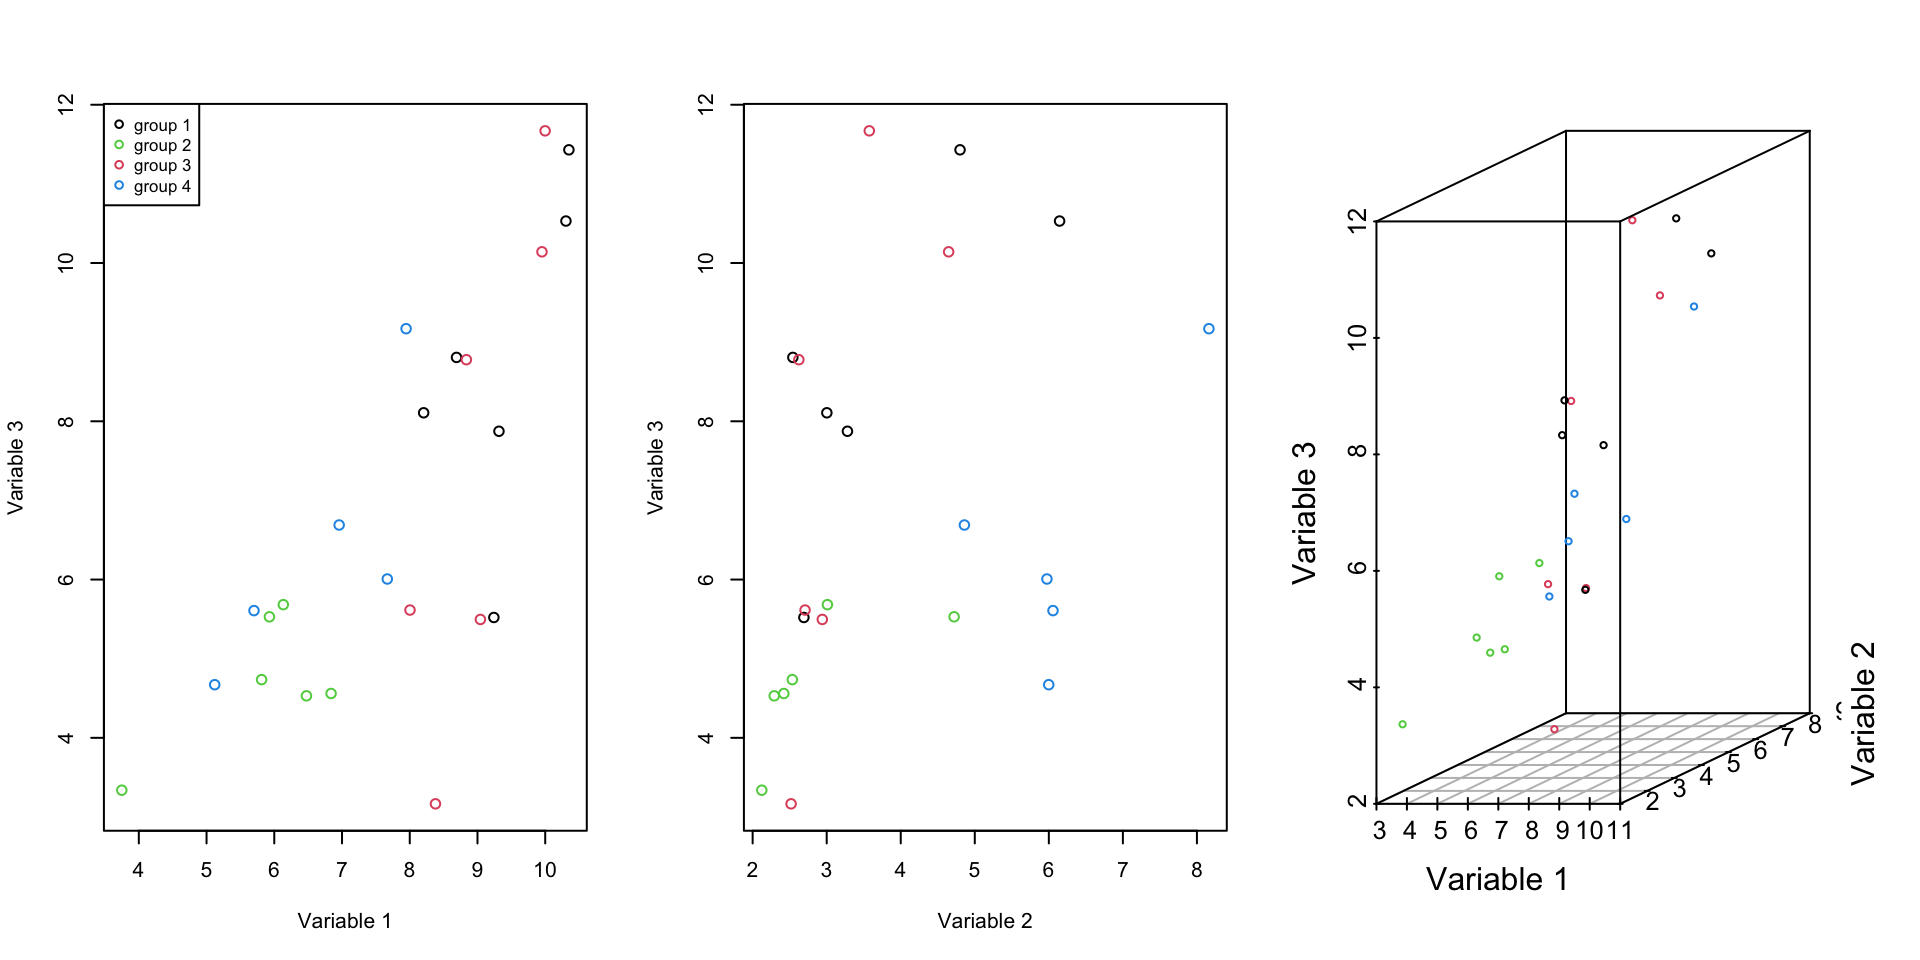
\includegraphics{PCA_files/figure-latex/fig-simple-cov3-1} 

}

\caption{Here, we select one of the previous variables and an additional one and show how the data is spread according to both of the variables.}\label{fig:fig-simple-cov3}
\end{figure}

The covariance of this new variable with the old ones is variable one: 3.4341536 and variable 2: 1.4907196. It is also obvious from the Figure \ref{fig:fig-simple-cov3} these new variable contain redundant information.

What about others? how kind of information do they contain? which ones are redundant which ones are complimentary? If we have to do the same analysis on the entire dataset, at best, we can repeat our analysis for three variables at a time, meaning that we will end up doing that 15288975159150 times! And how about if we should use more than 3 variables at the time to inspect the data pattern?

In fact, as the dimension of data (number of variables, e.g.~genes) increases, it becomes very difficult to draw conclusion from the data. We just cannot do that using simple methods. Fortunately, we have some amazing methods coming to rescue! This is the topic of the next chapter.

\hypertarget{pcamot}{%
\chapter{PCA (motivation)}\label{pcamot}}

\hypertarget{summary-of-the-previous-chapter}{%
\section{Summary of the previous chapter}\label{summary-of-the-previous-chapter}}

In the \protect\hyperlink{intro}{previous chapter}, we talked about two measures for summarizing our data, variation and covariation. Variation was used to measure the spread of a single variable whereas the covariation was between two variables measuring how much they agree with each other, thus showing the redundancy. We also emphasized that it is nice to have variables showing complimentary information rather than overlapping one! We also decided that, we want the variation of signal to be higher than the variation of noise. That is, probably the variables with higher variation are more interesting to us. We also show that the combination of two variables can give us more information about the data pattern, meaning that each of the variable contribute to the overall pattern. So to summarize:

\begin{itemize}
\tightlist
\item
  We agree that, we are interested in variation
\item
  We hope that the variation of signal is higher noise
\item
  By combining more variables together, we can probably get more information
\item
  There are redundancies between the different variables but we are mostly interested in the complimentary information they provide and to a lesser extend to the redundant information
\item
  We cannot manually handle a huge number of variable at the same time
\end{itemize}

\hypertarget{variation-and-covariation}{%
\section{Variation and covariation}\label{variation-and-covariation}}

This is a small point but so important that we put it under a separate heading. \textbf{Please note that variation and covariation are unbiased estimates.} This means that, they do not take into account the groupings/phenotype/meta data/other information about observations (samples). And we are going to agree that if \textbf{variable A} (a gene) has a variation of 2 and another \textbf{variable B} has a variation 1. We want to remain unbiased and give higher value to variable A compared to variable B EVEN if B shows us more ``true'' information about our experiment. So the higher the variation, the better, no matter what it shows. This might sound counterintuitive, but we will show that, remaining unbiased, will show us the data pattern that otherwise could not have been found.

\begin{itemize}
\tightlist
\item
  \textbf{So as of now, we are not going to show you labels of samples until when we want to interpret the data pattern}
\item
  \textbf{Remember: the higher the variation, the better}
\item
  \textbf{Variation of the data is how the data is spread, the bigger the spread the larger the variation}
\end{itemize}

\hypertarget{pcavar}{%
\section{Finding the largest variation}\label{pcavar}}

Let's start working on the same dataset. In the \protect\hyperlink{intro}{previous chapter}, we worked on maximum of three variables at the time (three axis: variable 1, 2, and 3). Twos variables showed high covariance. Let's plot them again. This time, without any colors!

\begin{Shaded}
\begin{Highlighting}[]
\CommentTok{# fix number of columns in the plot}
\KeywordTok{par}\NormalTok{(}\DataTypeTok{mfrow=}\KeywordTok{c}\NormalTok{(}\DecValTok{1}\NormalTok{,}\DecValTok{1}\NormalTok{))}
\CommentTok{# define variables}
\NormalTok{var1<-}\DecValTok{18924}
\NormalTok{var3<-}\DecValTok{18505}
\CommentTok{# plot the data}
\KeywordTok{plot}\NormalTok{(data[,}\KeywordTok{c}\NormalTok{(var1,var3)],}\DataTypeTok{xlab =} \StringTok{"Variable 1"}\NormalTok{, }\DataTypeTok{ylab =} \StringTok{"Variable 3"}\NormalTok{)}
\end{Highlighting}
\end{Shaded}

\begin{figure}

{\centering 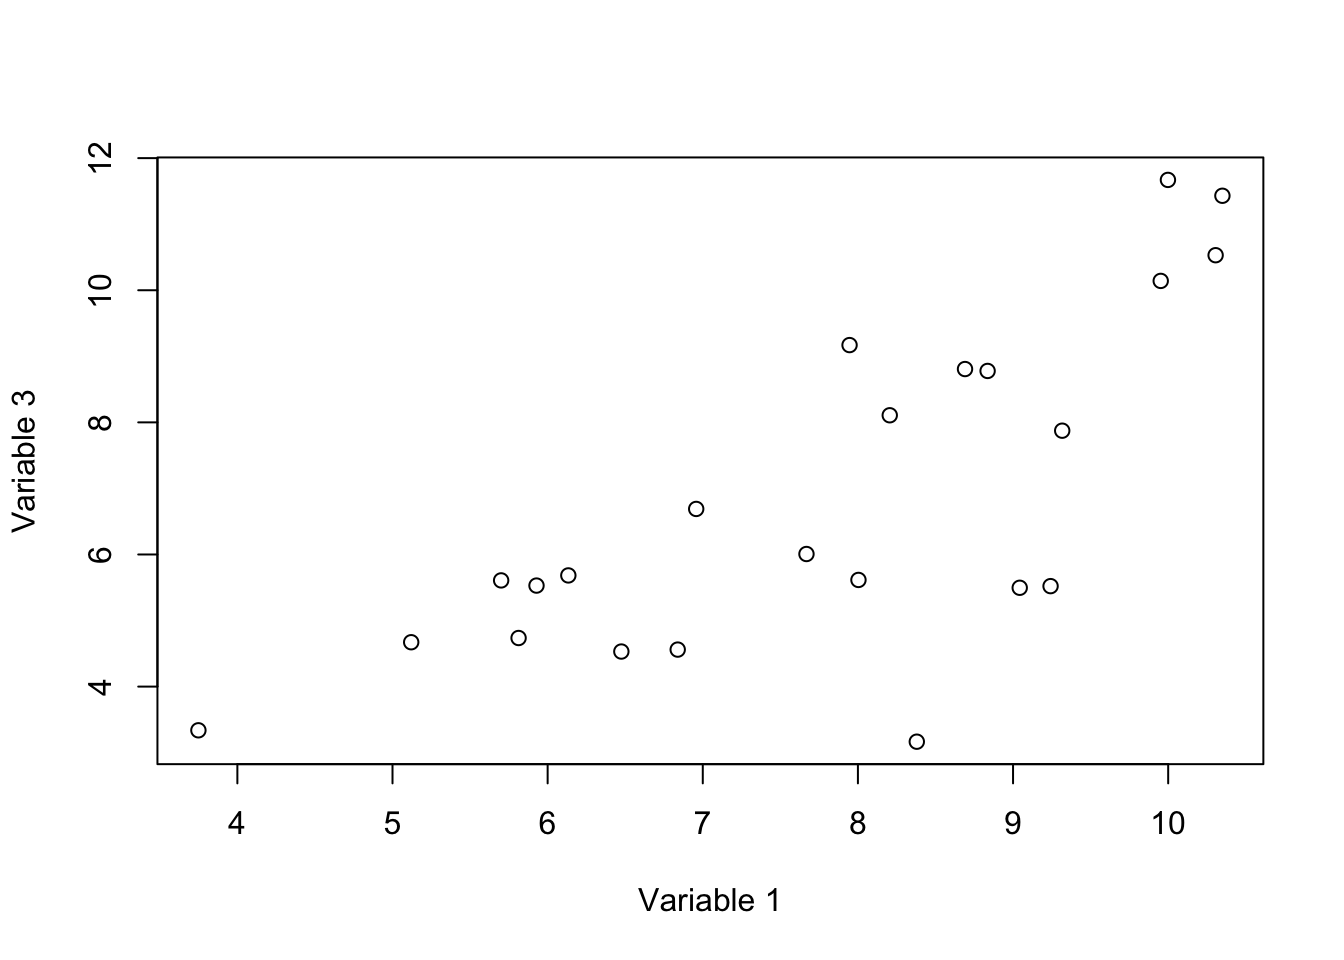
\includegraphics{PCA_files/figure-latex/fig-simple-cov4-1} 

}

\caption{Here, we select two variables and show how the data is spread according to the variables.}\label{fig:fig-simple-cov4}
\end{figure}

In \protect\hyperlink{fig-simple-cov4}{this figure}, we have two axis, x: variable 1 and y: variable 3. These two variables have high covariance (they change together). Each axis is obviously a line in which each of our observations has a location (or projection). For example for axis x:

\begin{Shaded}
\begin{Highlighting}[]
\CommentTok{# fix number of columns in the plot}
\KeywordTok{par}\NormalTok{(}\DataTypeTok{mfrow=}\KeywordTok{c}\NormalTok{(}\DecValTok{1}\NormalTok{,}\DecValTok{2}\NormalTok{))}
\CommentTok{# define variables}
\NormalTok{var1<-}\DecValTok{18924}
\NormalTok{var3<-}\DecValTok{18505}
\CommentTok{# plot the data}
\KeywordTok{plot}\NormalTok{(data[,}\KeywordTok{c}\NormalTok{(var1,var3)],}\DataTypeTok{xlab =} \StringTok{"Variable 1"}\NormalTok{, }\DataTypeTok{ylab =} \StringTok{"Variable 3"}\NormalTok{,}\DataTypeTok{axes =}\NormalTok{ F)}
\CommentTok{# draw the box}
\KeywordTok{box}\NormalTok{(}\DataTypeTok{col =} \StringTok{'black'}\NormalTok{)}
\CommentTok{# draw x axis}
\KeywordTok{axis}\NormalTok{(}\DecValTok{1}\NormalTok{, }\DataTypeTok{col =} \StringTok{'red'}\NormalTok{,}\DataTypeTok{cex=}\DecValTok{4}\NormalTok{)}
\CommentTok{# draw y axis}
\KeywordTok{axis}\NormalTok{(}\DecValTok{2}\NormalTok{)}

\CommentTok{# plot the arrows}
\ControlFlowTok{for}\NormalTok{(i }\ControlFlowTok{in} \DecValTok{1}\OperatorTok{:}\KeywordTok{nrow}\NormalTok{(data))}
\NormalTok{\{}
  \KeywordTok{arrows}\NormalTok{(}\DataTypeTok{x0 =}\KeywordTok{as.numeric}\NormalTok{( data[i,var1]),}\DataTypeTok{x1 =}\NormalTok{  data[i,var1],}
           \DataTypeTok{y0 =}\NormalTok{ data[i,var3],}\DataTypeTok{y1 =}\FloatTok{2.85}\NormalTok{,}\DataTypeTok{length=}\FloatTok{0.05}\NormalTok{,}\DataTypeTok{lty=}\StringTok{"dashed"}\NormalTok{)}
\NormalTok{\}}

\CommentTok{# plot the data}
\KeywordTok{plot}\NormalTok{(data[,}\KeywordTok{c}\NormalTok{(var1)],}\DataTypeTok{y=}\KeywordTok{rep}\NormalTok{(}\DecValTok{0}\NormalTok{,}\KeywordTok{nrow}\NormalTok{(data)),}\DataTypeTok{xlab =} \StringTok{"Variable 1"}\NormalTok{, }\DataTypeTok{ylab =} \StringTok{""}\NormalTok{,}\DataTypeTok{axes =}\NormalTok{ F)}
\CommentTok{# plot the axis}
\KeywordTok{axis}\NormalTok{(}\DecValTok{1}\NormalTok{, }\DataTypeTok{col =} \StringTok{'red'}\NormalTok{,}\DataTypeTok{cex=}\DecValTok{4}\NormalTok{,}\DataTypeTok{pos =} \KeywordTok{c}\NormalTok{(}\DecValTok{0}\NormalTok{,}\DecValTok{0}\NormalTok{),}\DataTypeTok{at =}\KeywordTok{unique}\NormalTok{(}\KeywordTok{c}\NormalTok{(}\KeywordTok{floor}\NormalTok{(data[,}\KeywordTok{c}\NormalTok{(var1)]),}\KeywordTok{ceiling}\NormalTok{(data[,}\KeywordTok{c}\NormalTok{(var1)]))) )}
\end{Highlighting}
\end{Shaded}

\begin{figure}

{\centering 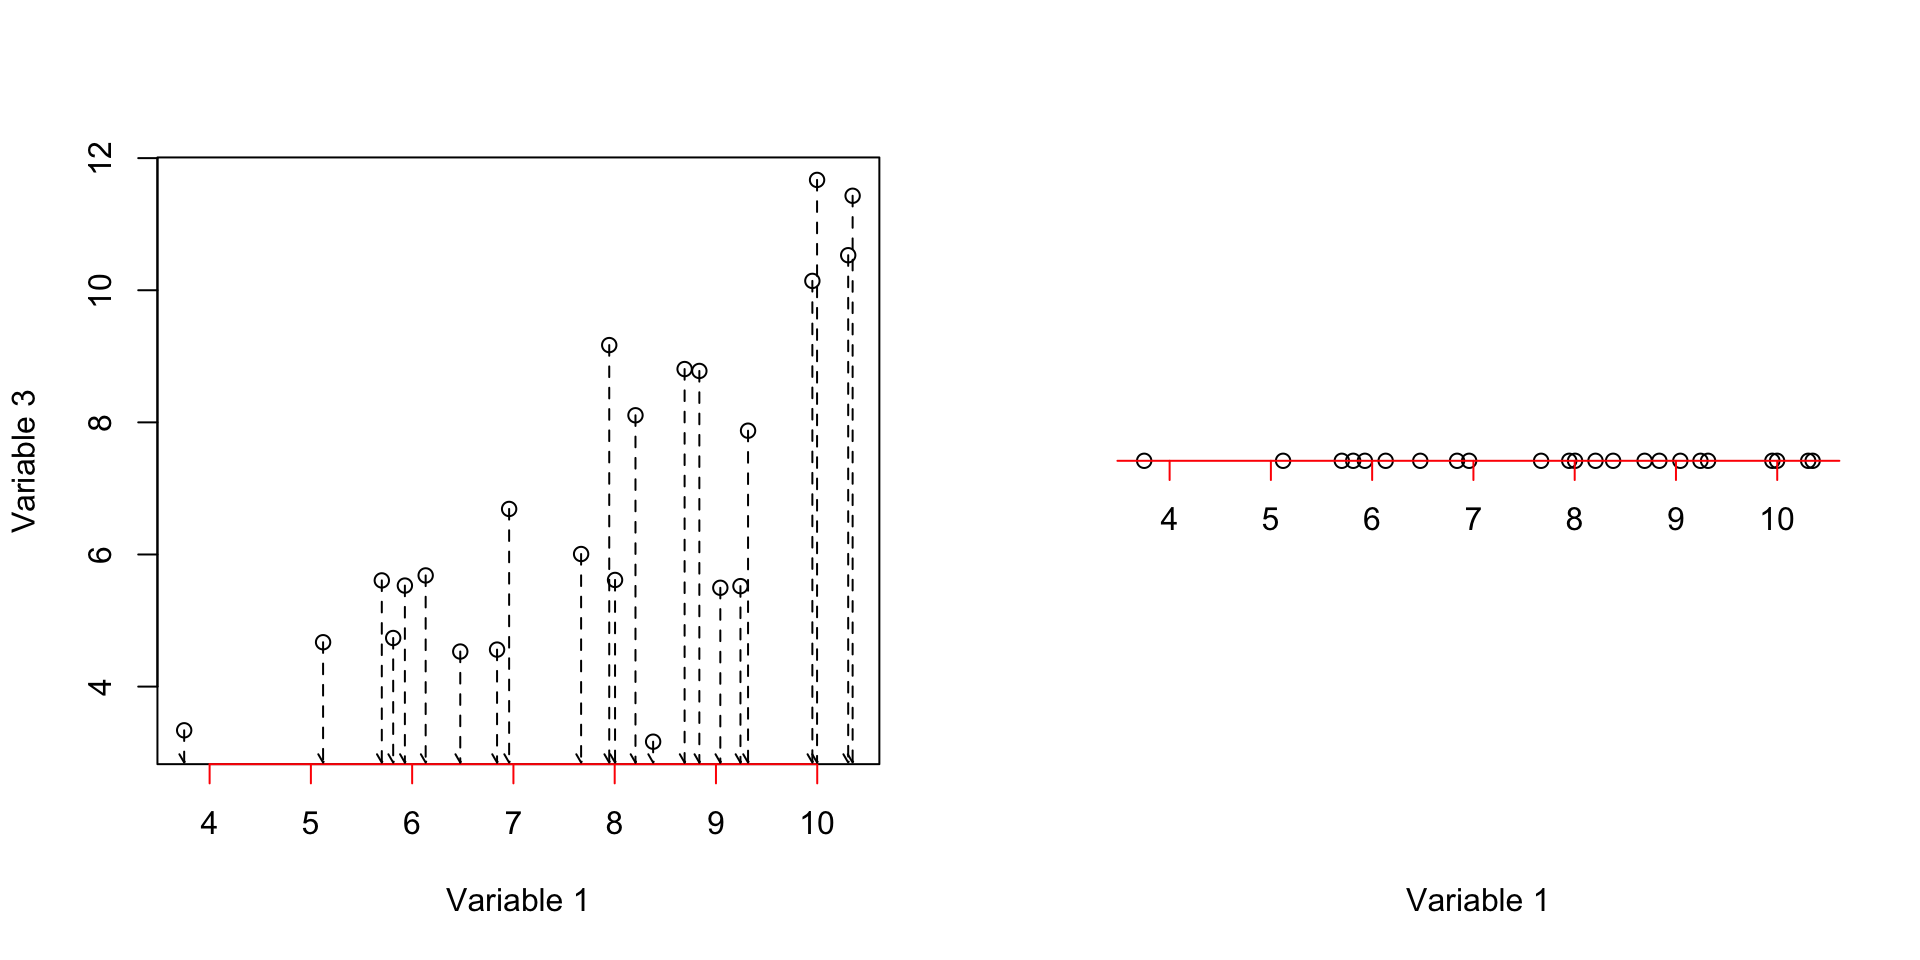
\includegraphics{PCA_files/figure-latex/fig-simple-location1-1} 

}

\caption{Here, we select two variables and show how the data is spread according to the variables. We show how the data is projected on the fist axis}\label{fig:fig-simple-location1}
\end{figure}

We can see in Figure \ref{fig:fig-simple-location1} (left panel), all of our observations have been mapped (projected) to the axis x (variable 1). The result is shown on the right plot. Obviously, it gives us the original values of observations in variable 1 with variation of 3.2822776. We could do the same thing for variable 3.

\begin{Shaded}
\begin{Highlighting}[]
\CommentTok{# fix number of columns in the plot}
\KeywordTok{par}\NormalTok{(}\DataTypeTok{mfrow=}\KeywordTok{c}\NormalTok{(}\DecValTok{1}\NormalTok{,}\DecValTok{2}\NormalTok{))}
\CommentTok{# define variables}
\NormalTok{var1<-}\DecValTok{18924}
\NormalTok{var3<-}\DecValTok{18505}
\CommentTok{# plot the data}
\KeywordTok{plot}\NormalTok{(data[,}\KeywordTok{c}\NormalTok{(var1,var3)],}\DataTypeTok{xlab =} \StringTok{"Variable 1"}\NormalTok{, }\DataTypeTok{ylab =} \StringTok{"Variable 3"}\NormalTok{,}\DataTypeTok{axes =}\NormalTok{ F)}
\CommentTok{# draw the box}
\KeywordTok{box}\NormalTok{(}\DataTypeTok{col =} \StringTok{'black'}\NormalTok{)}
\CommentTok{# draw y axis}
\KeywordTok{axis}\NormalTok{(}\DecValTok{2}\NormalTok{, }\DataTypeTok{col =} \StringTok{'red'}\NormalTok{,}\DataTypeTok{cex=}\DecValTok{4}\NormalTok{)}
\CommentTok{# draw x axis}
\KeywordTok{axis}\NormalTok{(}\DecValTok{1}\NormalTok{)}

\ControlFlowTok{for}\NormalTok{(i }\ControlFlowTok{in} \DecValTok{1}\OperatorTok{:}\KeywordTok{nrow}\NormalTok{(data))}
\NormalTok{\{}
  \KeywordTok{arrows}\NormalTok{(}\DataTypeTok{x0 =}\KeywordTok{as.numeric}\NormalTok{( data[i,var1]),}\DataTypeTok{x1 =}  \FloatTok{3.5}\NormalTok{,}
           \DataTypeTok{y0 =}\NormalTok{ data[i,var3],}\DataTypeTok{y1 =}\NormalTok{data[i,var3],}\DataTypeTok{length=}\FloatTok{0.05}\NormalTok{,}\DataTypeTok{lty=}\StringTok{"dashed"}\NormalTok{)}
\NormalTok{\}}

\CommentTok{# plot the data}
\KeywordTok{plot}\NormalTok{(}\DataTypeTok{x=}\KeywordTok{rep}\NormalTok{(}\DecValTok{0}\NormalTok{,}\KeywordTok{nrow}\NormalTok{(data)),}\DataTypeTok{y=}\NormalTok{data[,}\KeywordTok{c}\NormalTok{(var1)],}\DataTypeTok{xlab =} \StringTok{""}\NormalTok{, }\DataTypeTok{ylab =} \StringTok{"Variable 3"}\NormalTok{,}\DataTypeTok{axes =}\NormalTok{ F)}
\CommentTok{#plot the axis}
\KeywordTok{axis}\NormalTok{(}\DecValTok{2}\NormalTok{, }\DataTypeTok{col =} \StringTok{'red'}\NormalTok{,}\DataTypeTok{cex=}\DecValTok{4}\NormalTok{,}\DataTypeTok{pos =} \KeywordTok{c}\NormalTok{(}\DecValTok{0}\NormalTok{,}\DecValTok{0}\NormalTok{),}\DataTypeTok{at =}\KeywordTok{unique}\NormalTok{(}\KeywordTok{c}\NormalTok{(}\KeywordTok{floor}\NormalTok{(data[,}\KeywordTok{c}\NormalTok{(var3)]),}\KeywordTok{ceiling}\NormalTok{(data[,}\KeywordTok{c}\NormalTok{(var3)]))) )}
\end{Highlighting}
\end{Shaded}

\begin{figure}

{\centering 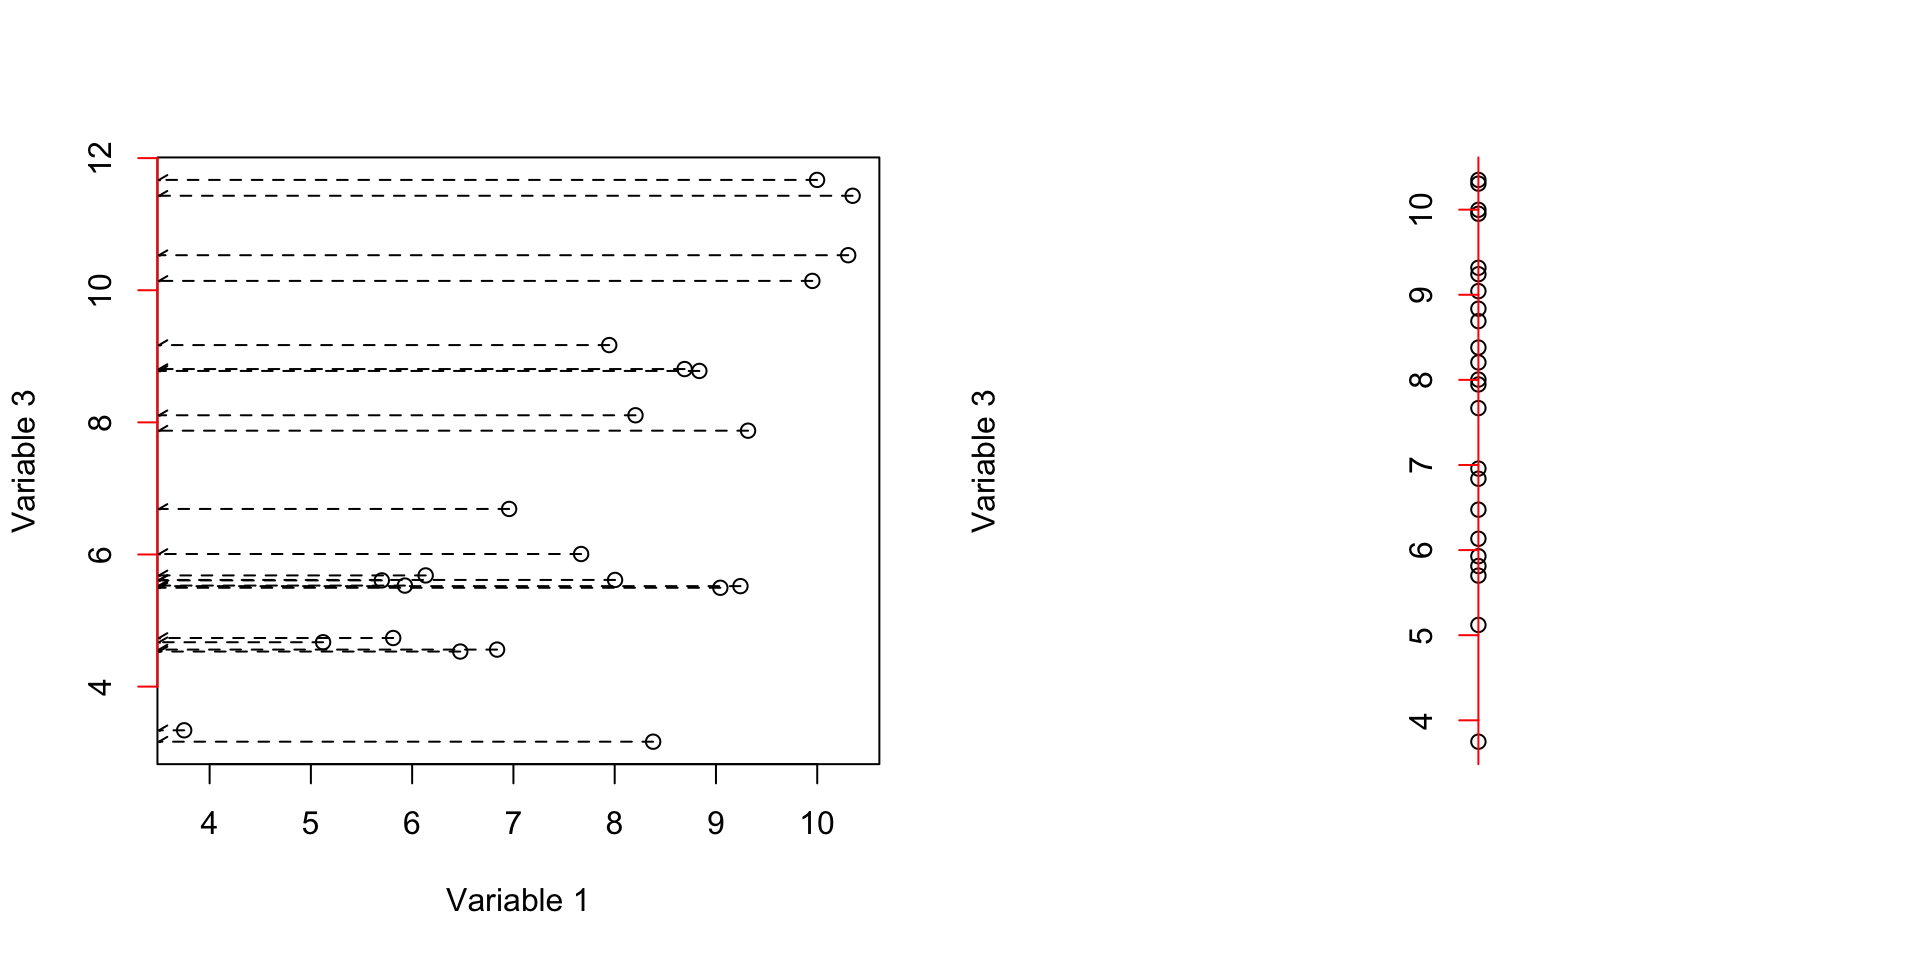
\includegraphics{PCA_files/figure-latex/fig-simple-location2-1} 

}

\caption{Here, we select two variables and show how the data is spread according to the variables. We show how the data is projected on the second axis}\label{fig:fig-simple-location2}
\end{figure}

This axis in Figure \ref{fig:fig-simple-location2} gave us variation of 6.3821145. The covariance of these two axis is 3.4341536.

\textbf{So to summarize, we draw two lines (axis) and mapped (projected the data points to these lines and measured the variance and covariance of the mapped data.}

Well, we are not limited to these lines! We can draw other lines. The idea is to come up with a line drawn through the data in a way that the projected data (orthogonal projection) has maximum variation. Let's try to see what it means in action by randomly draw a line

\begin{Shaded}
\begin{Highlighting}[]
\CommentTok{# fix number of columns in the plot}
\KeywordTok{par}\NormalTok{(}\DataTypeTok{mfrow=}\KeywordTok{c}\NormalTok{(}\DecValTok{1}\NormalTok{,}\DecValTok{2}\NormalTok{))}
\CommentTok{# define variables}
\NormalTok{var1<-}\DecValTok{18924}
\NormalTok{var3<-}\DecValTok{18505}
\CommentTok{# plot the data}
\KeywordTok{plot}\NormalTok{(data[,}\KeywordTok{c}\NormalTok{(var1,var3)],}\DataTypeTok{xlab =} \StringTok{"Variable 1"}\NormalTok{, }\DataTypeTok{ylab =} \StringTok{"Variable 3"}\NormalTok{,}\DataTypeTok{xlim =} \KeywordTok{c}\NormalTok{(}\DecValTok{2}\NormalTok{,}\DecValTok{15}\NormalTok{),}\DataTypeTok{ylim =} \KeywordTok{c}\NormalTok{(}\DecValTok{2}\NormalTok{,}\DecValTok{15}\NormalTok{))}
\CommentTok{# draw a line}
\CommentTok{# intercept}
\NormalTok{b<-}\FloatTok{2.5}
\CommentTok{# slope}
\NormalTok{m<-}\FloatTok{0.5}
\CommentTok{# draw the line}
\KeywordTok{abline}\NormalTok{(}\DataTypeTok{a =}\NormalTok{ b,}\DataTypeTok{b =}\NormalTok{ m,}\DataTypeTok{col=}\StringTok{"red"}\NormalTok{)}

\CommentTok{#}
\NormalTok{projected_variables<-}\KeywordTok{matrix}\NormalTok{(}\OtherTok{NA}\NormalTok{,}\DataTypeTok{nrow =} \KeywordTok{nrow}\NormalTok{(data),}\DataTypeTok{ncol =} \DecValTok{2}\NormalTok{)}
\ControlFlowTok{for}\NormalTok{(i }\ControlFlowTok{in} \DecValTok{1}\OperatorTok{:}\KeywordTok{nrow}\NormalTok{(data))}
\NormalTok{\{}

\CommentTok{# calculate the projection}
\NormalTok{l2 <-}\StringTok{ }\KeywordTok{c}\NormalTok{(}\DecValTok{1}\NormalTok{, m }\OperatorTok{+}\StringTok{ }\NormalTok{b)}
\NormalTok{l1 <-}\StringTok{ }\KeywordTok{c}\NormalTok{(}\DecValTok{0}\NormalTok{, b)}
\NormalTok{l1 <-}\StringTok{ }\KeywordTok{c}\NormalTok{(l1, }\DecValTok{0}\NormalTok{)}
\NormalTok{l2 <-}\StringTok{ }\KeywordTok{c}\NormalTok{(l2, }\DecValTok{0}\NormalTok{)}
\NormalTok{u <-}\StringTok{ }\KeywordTok{sum}\NormalTok{((}\KeywordTok{c}\NormalTok{(data[i,}\KeywordTok{c}\NormalTok{(var1,var3)],}\DecValTok{0}\NormalTok{) }\OperatorTok{-}\StringTok{ }\NormalTok{l1)}\OperatorTok{*}\NormalTok{(l2 }\OperatorTok{-}\StringTok{ }\NormalTok{l1)) }\OperatorTok{/}\StringTok{ }\KeywordTok{sum}\NormalTok{((l2 }\OperatorTok{-}\StringTok{ }\NormalTok{l1)}\OperatorTok{^}\DecValTok{2}\NormalTok{)}
\NormalTok{r<-l1 }\OperatorTok{+}\StringTok{ }\NormalTok{u }\OperatorTok{*}\StringTok{ }\NormalTok{(l2 }\OperatorTok{-}\StringTok{ }\NormalTok{l1)}
\CommentTok{# end projection}

\CommentTok{# draw arrow}
  \KeywordTok{arrows}\NormalTok{(}\DataTypeTok{x0 =}\NormalTok{ data[i,var1],}\DataTypeTok{x1 =}\NormalTok{ r[}\DecValTok{1}\NormalTok{],}
           \DataTypeTok{y0 =}\NormalTok{ data[i,var3],}\DataTypeTok{y1 =}\NormalTok{r[}\DecValTok{2}\NormalTok{],}\DataTypeTok{length=}\FloatTok{0.05}\NormalTok{,}\DataTypeTok{lty=}\StringTok{"dashed"}\NormalTok{)}


\CommentTok{# save the projections}
\NormalTok{projected_variables[i,}\DecValTok{1}\NormalTok{]<-r[}\DecValTok{1}\NormalTok{]}
\NormalTok{projected_variables[i,}\DecValTok{2}\NormalTok{]<-r[}\DecValTok{2}\NormalTok{]}

\NormalTok{\}}



\KeywordTok{plot}\NormalTok{(projected_variables,}\DataTypeTok{xlab =} \StringTok{"Variable 1"}\NormalTok{, }\DataTypeTok{ylab =} \StringTok{"Variable 3"}\NormalTok{,}\DataTypeTok{xlim =} \KeywordTok{c}\NormalTok{(}\DecValTok{2}\NormalTok{,}\DecValTok{15}\NormalTok{),}\DataTypeTok{ylim =} \KeywordTok{c}\NormalTok{(}\DecValTok{2}\NormalTok{,}\DecValTok{15}\NormalTok{))}
\KeywordTok{abline}\NormalTok{(}\DataTypeTok{a =}\NormalTok{ b,}\DataTypeTok{b =}\NormalTok{ m,}\DataTypeTok{col=}\StringTok{"red"}\NormalTok{)}
\end{Highlighting}
\end{Shaded}

\begin{figure}

{\centering 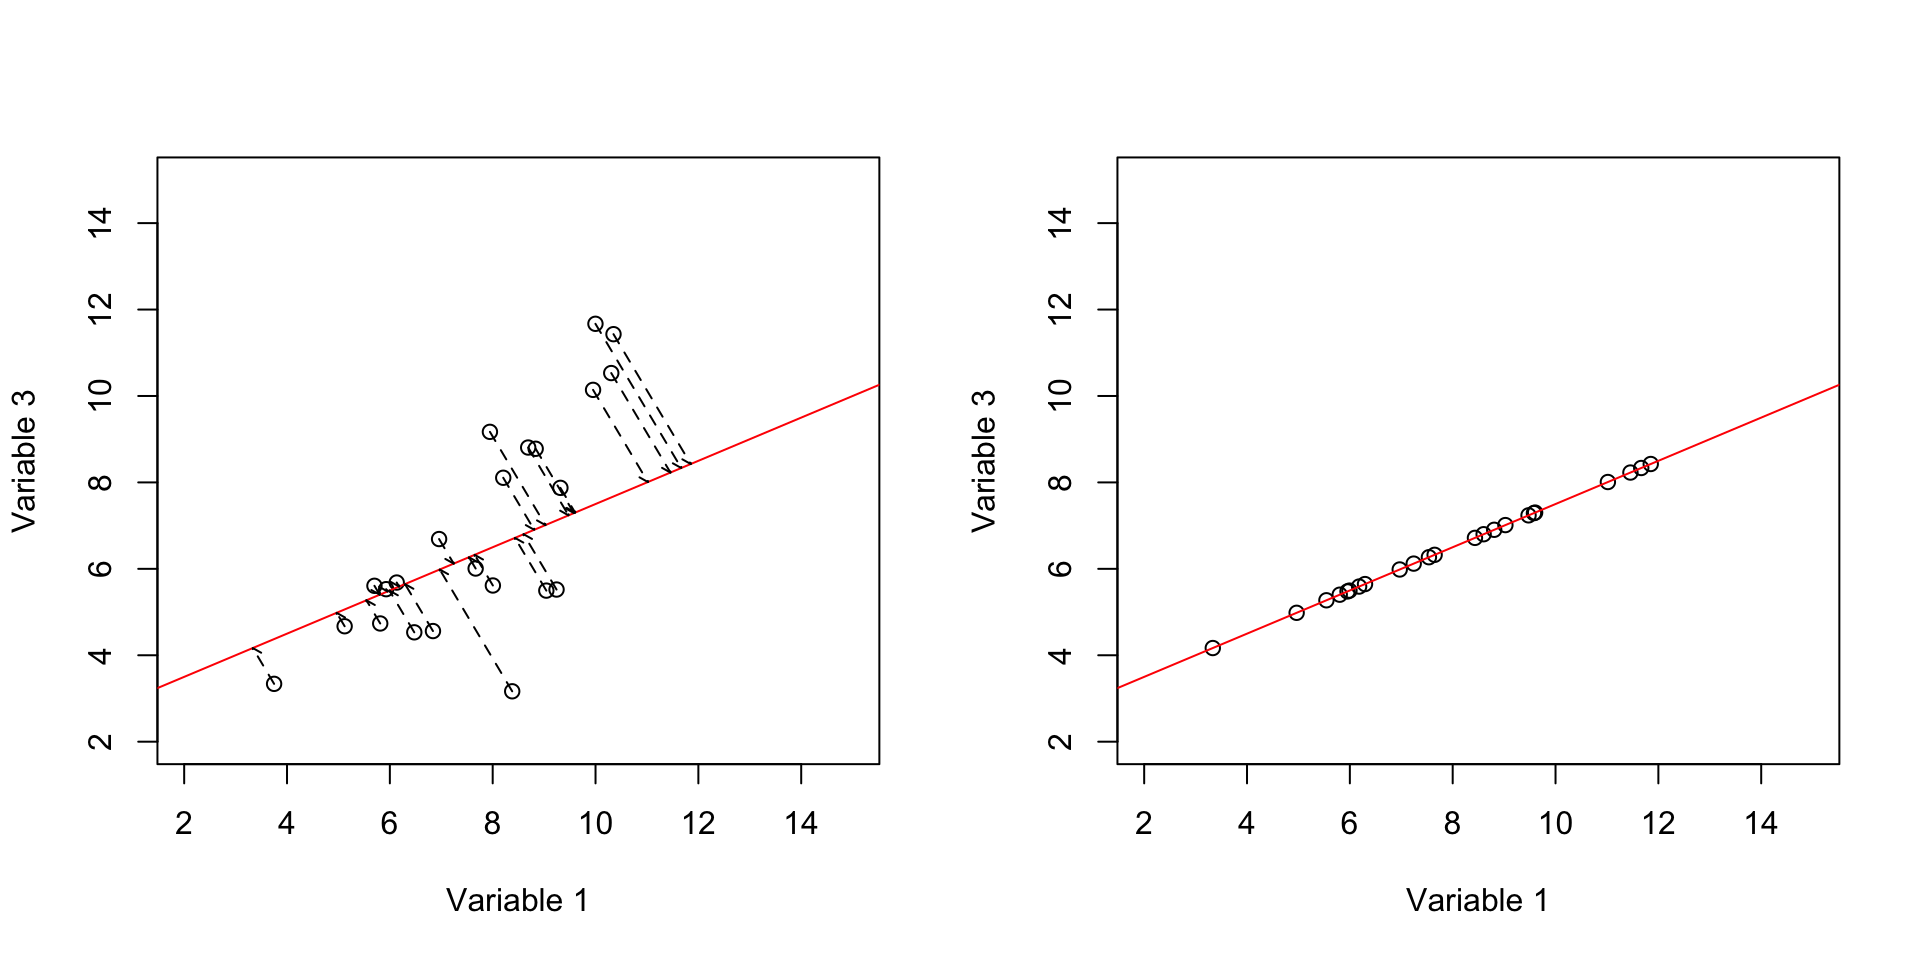
\includegraphics{PCA_files/figure-latex/fig-simple-line1-1} 

}

\caption{Here, we select two variables and show how the data is spread according to the variables. We draw a line through the data and project the data on that line and then measure the variance.}\label{fig:fig-simple-line1}
\end{figure}

\begin{Shaded}
\begin{Highlighting}[]
\CommentTok{#plot(x=apply(projected_variables,1,mean),y=rep(0,nrow(data)))}
\end{Highlighting}
\end{Shaded}

So in Figure \ref{fig:fig-simple-line1} we have drawn an arbitrary line (left panel) and put everything on that line (right panel). It might be a bit confusing. But let's rotate that red line so it becomes horizontal exactly line x axis.

\begin{Shaded}
\begin{Highlighting}[]
\CommentTok{# set number of figures in a plot}
\KeywordTok{par}\NormalTok{(}\DataTypeTok{mfrow=}\KeywordTok{c}\NormalTok{(}\DecValTok{1}\NormalTok{,}\DecValTok{1}\NormalTok{))}


\KeywordTok{plot}\NormalTok{(}\DataTypeTok{x=}\KeywordTok{apply}\NormalTok{(projected_variables,}\DecValTok{1}\NormalTok{,mean),}\DataTypeTok{y=}\KeywordTok{rep}\NormalTok{(}\DecValTok{0}\NormalTok{,}\KeywordTok{nrow}\NormalTok{(data)),}\DataTypeTok{axes =}\NormalTok{ F,}\DataTypeTok{ylab =} \StringTok{""}\NormalTok{,}\DataTypeTok{xlab =} \StringTok{"Combined variable 1 and 3"}\NormalTok{)}
\KeywordTok{axis}\NormalTok{(}\DecValTok{1}\NormalTok{, }\DataTypeTok{col =} \StringTok{'red'}\NormalTok{,}\DataTypeTok{cex=}\DecValTok{4}\NormalTok{,}\DataTypeTok{pos =} \KeywordTok{c}\NormalTok{(}\DecValTok{0}\NormalTok{,}\DecValTok{0}\NormalTok{),}\DataTypeTok{at =}\KeywordTok{unique}\NormalTok{(}\KeywordTok{c}\NormalTok{(}\KeywordTok{floor}\NormalTok{(}\KeywordTok{apply}\NormalTok{(projected_variables,}\DecValTok{1}\NormalTok{,mean)),}\KeywordTok{ceiling}\NormalTok{(}\KeywordTok{apply}\NormalTok{(projected_variables,}\DecValTok{1}\NormalTok{,mean)))) )}
\end{Highlighting}
\end{Shaded}

\begin{figure}

{\centering 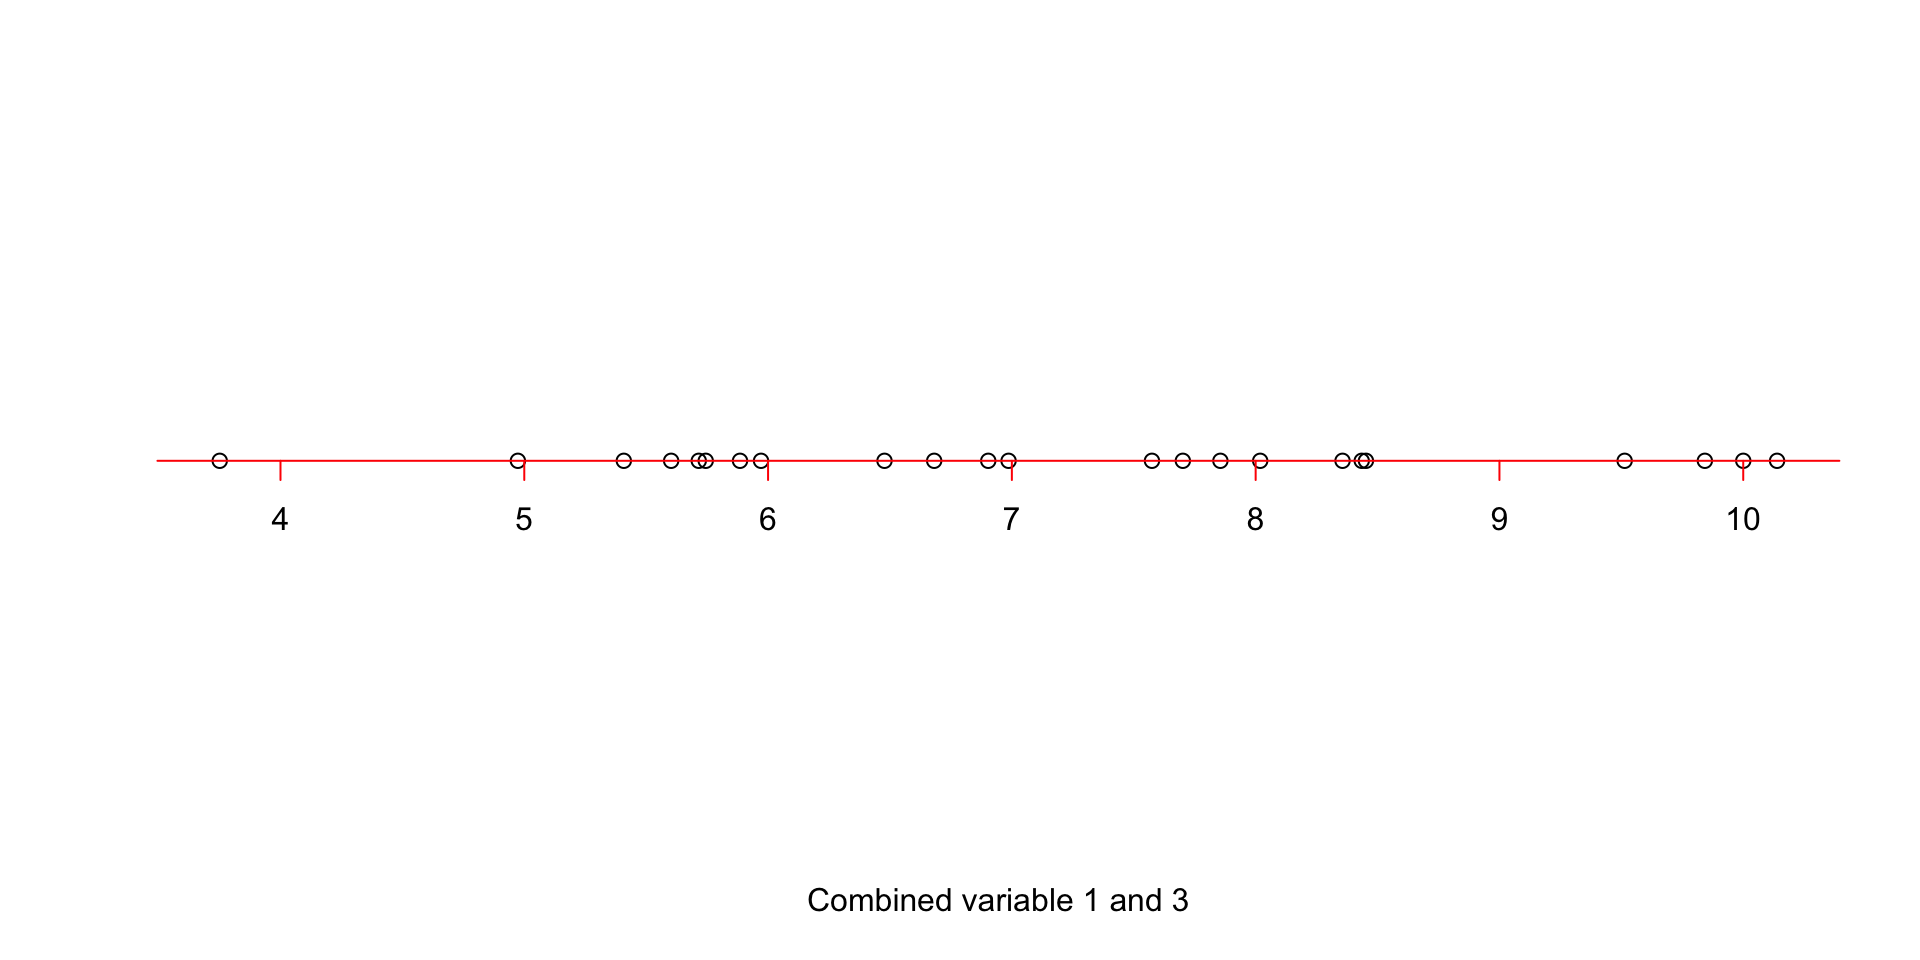
\includegraphics{PCA_files/figure-latex/fig-simple-line2-1} 

}

\caption{Simple rotation of the projected points on the line}\label{fig:fig-simple-line2}
\end{figure}

Figure \ref{fig:fig-simple-line2} shows our new x axis. If fact, this is a new variable! It's not quite variable 1, it's not variable 3, but a combination of these two. What is the variation of this new variable?! The variation is: 2.9923055. Well, that is great! But the question is, we can draw as many lines as we want, what should we do? Let's, imagine that we can try infinite possibilities. Which line would you select?

\begin{Shaded}
\begin{Highlighting}[]
\CommentTok{# fix number of columns in the plot}
\KeywordTok{par}\NormalTok{(}\DataTypeTok{mfrow=}\KeywordTok{c}\NormalTok{(}\DecValTok{1}\NormalTok{,}\DecValTok{3}\NormalTok{))}
\CommentTok{# define variables}
\NormalTok{var1<-}\DecValTok{18924}
\NormalTok{var3<-}\DecValTok{18505}
\CommentTok{# plot the data}
\KeywordTok{plot}\NormalTok{(data[,}\KeywordTok{c}\NormalTok{(var1,var3)],}\DataTypeTok{xlab =} \StringTok{"Variable 1"}\NormalTok{, }\DataTypeTok{ylab =} \StringTok{"Variable 3"}\NormalTok{,}\DataTypeTok{xlim =} \KeywordTok{c}\NormalTok{(}\DecValTok{2}\NormalTok{,}\DecValTok{15}\NormalTok{),}\DataTypeTok{ylim =} \KeywordTok{c}\NormalTok{(}\DecValTok{2}\NormalTok{,}\DecValTok{15}\NormalTok{))}
\CommentTok{# draw a line}
\CommentTok{# intercept}
\NormalTok{b<-}\FloatTok{2.5}
\CommentTok{# slope}
\NormalTok{m<-}\FloatTok{0.5}

\CommentTok{# draw many lines using different slope and intercept}
\ControlFlowTok{for}\NormalTok{(b }\ControlFlowTok{in} \KeywordTok{c}\NormalTok{(}\DecValTok{1}\OperatorTok{:}\DecValTok{5}\NormalTok{))}
\NormalTok{\{}
  \ControlFlowTok{for}\NormalTok{(m }\ControlFlowTok{in} \KeywordTok{seq}\NormalTok{(}\DecValTok{0}\NormalTok{,}\DecValTok{1}\NormalTok{,}\DataTypeTok{by=}\FloatTok{0.1}\NormalTok{))}
\NormalTok{  \{}
    \KeywordTok{abline}\NormalTok{(}\DataTypeTok{a =}\NormalTok{ b,}\DataTypeTok{b =}\NormalTok{ m,}\DataTypeTok{col=}\StringTok{"red"}\NormalTok{)}
\NormalTok{  \}}
\NormalTok{\}}

\CommentTok{# intercept}
\NormalTok{b<-}\OperatorTok{-}\FloatTok{5.172751}
\CommentTok{# slope}
\NormalTok{m<-}\FloatTok{1.548455}
\CommentTok{# draw the line}
\KeywordTok{abline}\NormalTok{(}\DataTypeTok{a =}\NormalTok{ b,}\DataTypeTok{b =}\NormalTok{ m,}\DataTypeTok{col=}\StringTok{"blue"}\NormalTok{,}\DataTypeTok{lwd =} \DecValTok{2}\NormalTok{)}


\KeywordTok{plot}\NormalTok{(data[,}\KeywordTok{c}\NormalTok{(var1,var3)],}\DataTypeTok{xlab =} \StringTok{"Variable 1"}\NormalTok{, }\DataTypeTok{ylab =} \StringTok{"Variable 3"}\NormalTok{,}\DataTypeTok{xlim =} \KeywordTok{c}\NormalTok{(}\DecValTok{2}\NormalTok{,}\DecValTok{15}\NormalTok{),}\DataTypeTok{ylim =} \KeywordTok{c}\NormalTok{(}\DecValTok{2}\NormalTok{,}\DecValTok{15}\NormalTok{))}

\CommentTok{# draw the line}
\KeywordTok{abline}\NormalTok{(}\DataTypeTok{a =}\NormalTok{ b,}\DataTypeTok{b =}\NormalTok{ m,}\DataTypeTok{col=}\StringTok{"blue"}\NormalTok{)}


\CommentTok{#}
\NormalTok{projected_variables<-}\KeywordTok{matrix}\NormalTok{(}\OtherTok{NA}\NormalTok{,}\DataTypeTok{nrow =} \KeywordTok{nrow}\NormalTok{(data),}\DataTypeTok{ncol =} \DecValTok{2}\NormalTok{)}
\ControlFlowTok{for}\NormalTok{(i }\ControlFlowTok{in} \DecValTok{1}\OperatorTok{:}\KeywordTok{nrow}\NormalTok{(data))}
\NormalTok{\{}

\CommentTok{# calculate the projection}
\NormalTok{l2 <-}\StringTok{ }\KeywordTok{c}\NormalTok{(}\DecValTok{1}\NormalTok{, m }\OperatorTok{+}\StringTok{ }\NormalTok{b)}
\NormalTok{l1 <-}\StringTok{ }\KeywordTok{c}\NormalTok{(}\DecValTok{0}\NormalTok{, b)}
\NormalTok{l1 <-}\StringTok{ }\KeywordTok{c}\NormalTok{(l1, }\DecValTok{0}\NormalTok{)}
\NormalTok{l2 <-}\StringTok{ }\KeywordTok{c}\NormalTok{(l2, }\DecValTok{0}\NormalTok{)}
\NormalTok{u <-}\StringTok{ }\KeywordTok{sum}\NormalTok{((}\KeywordTok{c}\NormalTok{(data[i,}\KeywordTok{c}\NormalTok{(var1,var3)],}\DecValTok{0}\NormalTok{) }\OperatorTok{-}\StringTok{ }\NormalTok{l1)}\OperatorTok{*}\NormalTok{(l2 }\OperatorTok{-}\StringTok{ }\NormalTok{l1)) }\OperatorTok{/}\StringTok{ }\KeywordTok{sum}\NormalTok{((l2 }\OperatorTok{-}\StringTok{ }\NormalTok{l1)}\OperatorTok{^}\DecValTok{2}\NormalTok{)}
\NormalTok{r<-l1 }\OperatorTok{+}\StringTok{ }\NormalTok{u }\OperatorTok{*}\StringTok{ }\NormalTok{(l2 }\OperatorTok{-}\StringTok{ }\NormalTok{l1)}
\CommentTok{# end projection}

\CommentTok{# draw arrow}
  \KeywordTok{arrows}\NormalTok{(}\DataTypeTok{x0 =}\NormalTok{ data[i,var1],}\DataTypeTok{x1 =}\NormalTok{ r[}\DecValTok{1}\NormalTok{],}
           \DataTypeTok{y0 =}\NormalTok{ data[i,var3],}\DataTypeTok{y1 =}\NormalTok{r[}\DecValTok{2}\NormalTok{],}\DataTypeTok{length=}\FloatTok{0.05}\NormalTok{,}\DataTypeTok{lty=}\StringTok{"dashed"}\NormalTok{)}


\CommentTok{# save the projections}
\NormalTok{projected_variables[i,}\DecValTok{1}\NormalTok{]<-r[}\DecValTok{1}\NormalTok{]}
\NormalTok{projected_variables[i,}\DecValTok{2}\NormalTok{]<-r[}\DecValTok{2}\NormalTok{]}

\NormalTok{\}}

\CommentTok{# save projection direction (came from svd)}
\NormalTok{projection_directions<-}\KeywordTok{matrix}\NormalTok{(}\KeywordTok{c}\NormalTok{(}\OperatorTok{-}\FloatTok{0.5425087359}\NormalTok{ ,}\OperatorTok{-}\FloatTok{0.8400501601}\NormalTok{,}\OperatorTok{-}\FloatTok{0.8400501601}\NormalTok{,}\FloatTok{0.5425087359}\NormalTok{),}\DataTypeTok{nrow =} \DecValTok{2}\NormalTok{)}

 

\CommentTok{# decenter data}
\NormalTok{decenter_data<-}\KeywordTok{scale}\NormalTok{((}\KeywordTok{scale}\NormalTok{(data[,}\KeywordTok{c}\NormalTok{(var1,var3)],}\DataTypeTok{scale =}\NormalTok{ F))}\OperatorTok\NormalTok{projection_directions, }\DataTypeTok{scale =} \OtherTok{FALSE}\NormalTok{, }\DataTypeTok{center =} \DecValTok{-1} \OperatorTok{*}\StringTok{ }\KeywordTok{c}\NormalTok{(}\FloatTok{7.767432}\NormalTok{,}\FloatTok{6.854765}\NormalTok{))}


\CommentTok{# plot the data}
\KeywordTok{plot}\NormalTok{(}\DataTypeTok{x=}\NormalTok{decenter_data[,}\DecValTok{1}\NormalTok{],}\DataTypeTok{y=}\KeywordTok{rep}\NormalTok{(}\DecValTok{0}\NormalTok{,}\KeywordTok{nrow}\NormalTok{(data)),}\DataTypeTok{axes =}\NormalTok{ F,}\DataTypeTok{ylab =} \StringTok{""}\NormalTok{,}\DataTypeTok{xlab =} \StringTok{"Combined variable 1 and 3"}\NormalTok{)}


\KeywordTok{axis}\NormalTok{(}\DecValTok{1}\NormalTok{, }\DataTypeTok{col =} \StringTok{'blue'}\NormalTok{,}\DataTypeTok{cex=}\DecValTok{4}\NormalTok{,}\DataTypeTok{pos =} \KeywordTok{c}\NormalTok{(}\DecValTok{0}\NormalTok{,}\DecValTok{0}\NormalTok{),}\DataTypeTok{at =}\KeywordTok{unique}\NormalTok{(}\KeywordTok{c}\NormalTok{(}\KeywordTok{floor}\NormalTok{(decenter_data[,}\DecValTok{1}\NormalTok{]),}\KeywordTok{ceiling}\NormalTok{(decenter_data[,}\DecValTok{1}\NormalTok{]))) )}
\end{Highlighting}
\end{Shaded}

\begin{figure}

{\centering 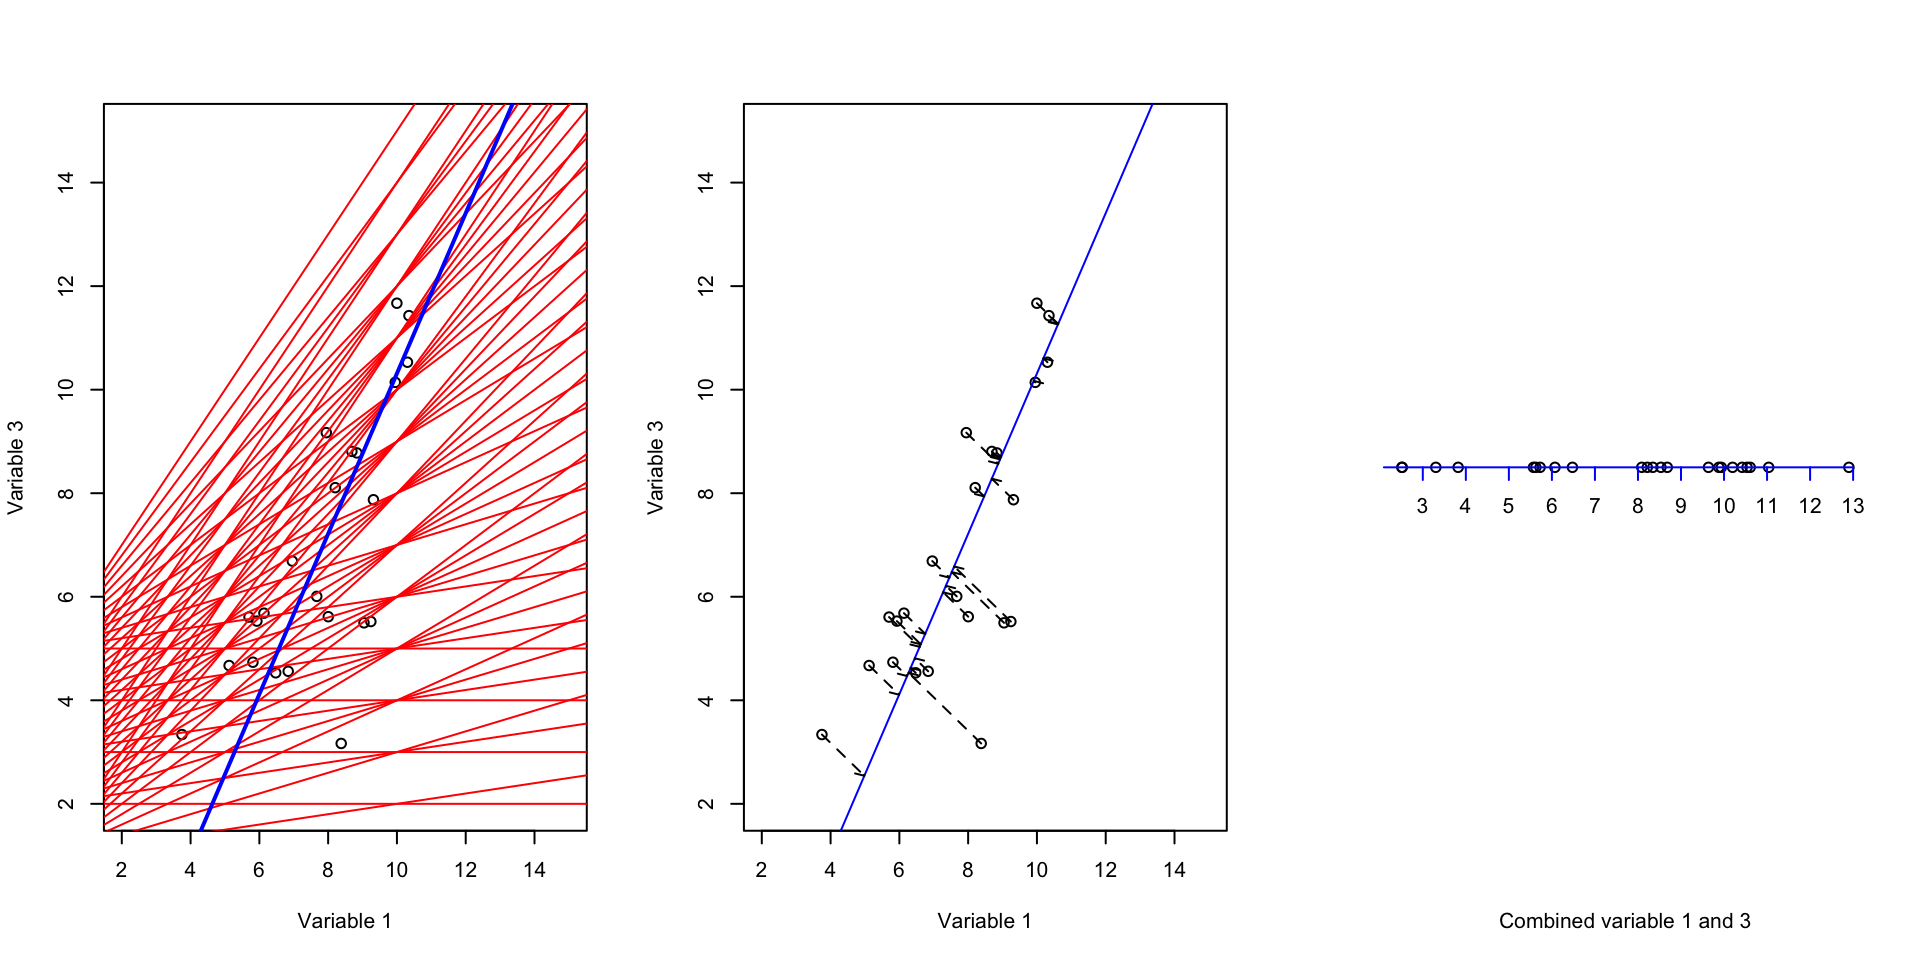
\includegraphics{PCA_files/figure-latex/fig-simple-line3-1} 

}

\caption{We try to fit many lines through the data but there is only one of the lines that capture most of the variance}\label{fig:fig-simple-line3}
\end{figure}

Intuitively, one would select a line that has the maximum variation. That is the blue line. Variation of this line is 8.5999087 that is the highest amount all other lines that can be drawn. By now, we have a new variable that is a combination the original two variables and has captured most of the variation. But how about the remaining variation? What should we do about the redundancy?

So ideally what we want to do is to come up with another line that when we mapped the data on it, it captures the remaining variation but also \textbf{avoid redundancy}. Last point means that the covariance between the observations that we have already mapped to the first line (the blue line in Figure \ref{fig:fig-simple-line3}) and the observations that we mapped on this new line should be \textbf{zero} or \textbf{very close to zero}.

It turns out that the only way of finding such a line is to find the line that is orthogonal to the first line (the blue line in Figure \ref{fig:fig-simple-line3}). Orthogonal means that the angle of this new line to the blue on should be exactly 90 degree:

\begin{Shaded}
\begin{Highlighting}[]
\CommentTok{# set number of plots to 1}
\KeywordTok{par}\NormalTok{(}\DataTypeTok{mfrow=}\KeywordTok{c}\NormalTok{(}\DecValTok{1}\NormalTok{,}\DecValTok{1}\NormalTok{))}
\CommentTok{# plot an empty plot}
\KeywordTok{plot}\NormalTok{(}\DecValTok{1}\NormalTok{,}\DataTypeTok{type=}\StringTok{"n"}\NormalTok{,}\DataTypeTok{axes=}\NormalTok{F,}\DataTypeTok{xlim=}\KeywordTok{c}\NormalTok{(}\OperatorTok{-}\FloatTok{0.1}\NormalTok{,}\FloatTok{1.2}\NormalTok{),}\DataTypeTok{ylim=}\KeywordTok{c}\NormalTok{(}\OperatorTok{-}\FloatTok{0.1}\NormalTok{,}\FloatTok{1.2}\NormalTok{),}\DataTypeTok{xlab=}\StringTok{""}\NormalTok{,}\DataTypeTok{ylab=}\StringTok{""}\NormalTok{)}

\CommentTok{# define axis}
\NormalTok{x1 =}\StringTok{ }\KeywordTok{c}\NormalTok{(}\DecValTok{1}\NormalTok{,}\DecValTok{0}\NormalTok{)}
\NormalTok{x2 =}\StringTok{ }\KeywordTok{c}\NormalTok{(}\DecValTok{0}\NormalTok{,}\DecValTok{1}\NormalTok{)}

\CommentTok{# plot x arrow}
\KeywordTok{arrows}\NormalTok{(}\DecValTok{0}\NormalTok{,}\DecValTok{0}\NormalTok{,x1[}\DecValTok{1}\NormalTok{],x1[}\DecValTok{2}\NormalTok{])}


\CommentTok{# plot y arrow}
\KeywordTok{arrows}\NormalTok{(}\DecValTok{0}\NormalTok{,}\DecValTok{0}\NormalTok{,x2[}\DecValTok{1}\NormalTok{],x2[}\DecValTok{2}\NormalTok{])}

\CommentTok{# draw angle }
\KeywordTok{segments}\NormalTok{(}\DataTypeTok{x0 =} \FloatTok{0.1}\NormalTok{,}\DataTypeTok{y0 =} \DecValTok{0}\NormalTok{,}\DataTypeTok{x1 =} \FloatTok{0.1}\NormalTok{,}\DataTypeTok{y1 =} \FloatTok{0.1}\NormalTok{)}
\KeywordTok{segments}\NormalTok{(}\DataTypeTok{x0 =} \DecValTok{0}\NormalTok{,}\DataTypeTok{y0 =} \FloatTok{0.1}\NormalTok{,}\DataTypeTok{x1 =} \FloatTok{0.1}\NormalTok{,}\DataTypeTok{y1 =} \FloatTok{0.1}\NormalTok{)}

\CommentTok{# draw arrow to the text}
\KeywordTok{arrows}\NormalTok{(}\DecValTok{0}\NormalTok{,}\DecValTok{0}\NormalTok{,}\FloatTok{0.17}\NormalTok{,}\FloatTok{0.17}\NormalTok{)}

\CommentTok{# write text}
\KeywordTok{text}\NormalTok{(}\FloatTok{0.4}\NormalTok{,}\FloatTok{0.2}\NormalTok{,}\StringTok{"This angle is 90 degree"}\NormalTok{,}\DataTypeTok{cex=}\FloatTok{1.5}\NormalTok{)}
\end{Highlighting}
\end{Shaded}

\begin{figure}

{\centering 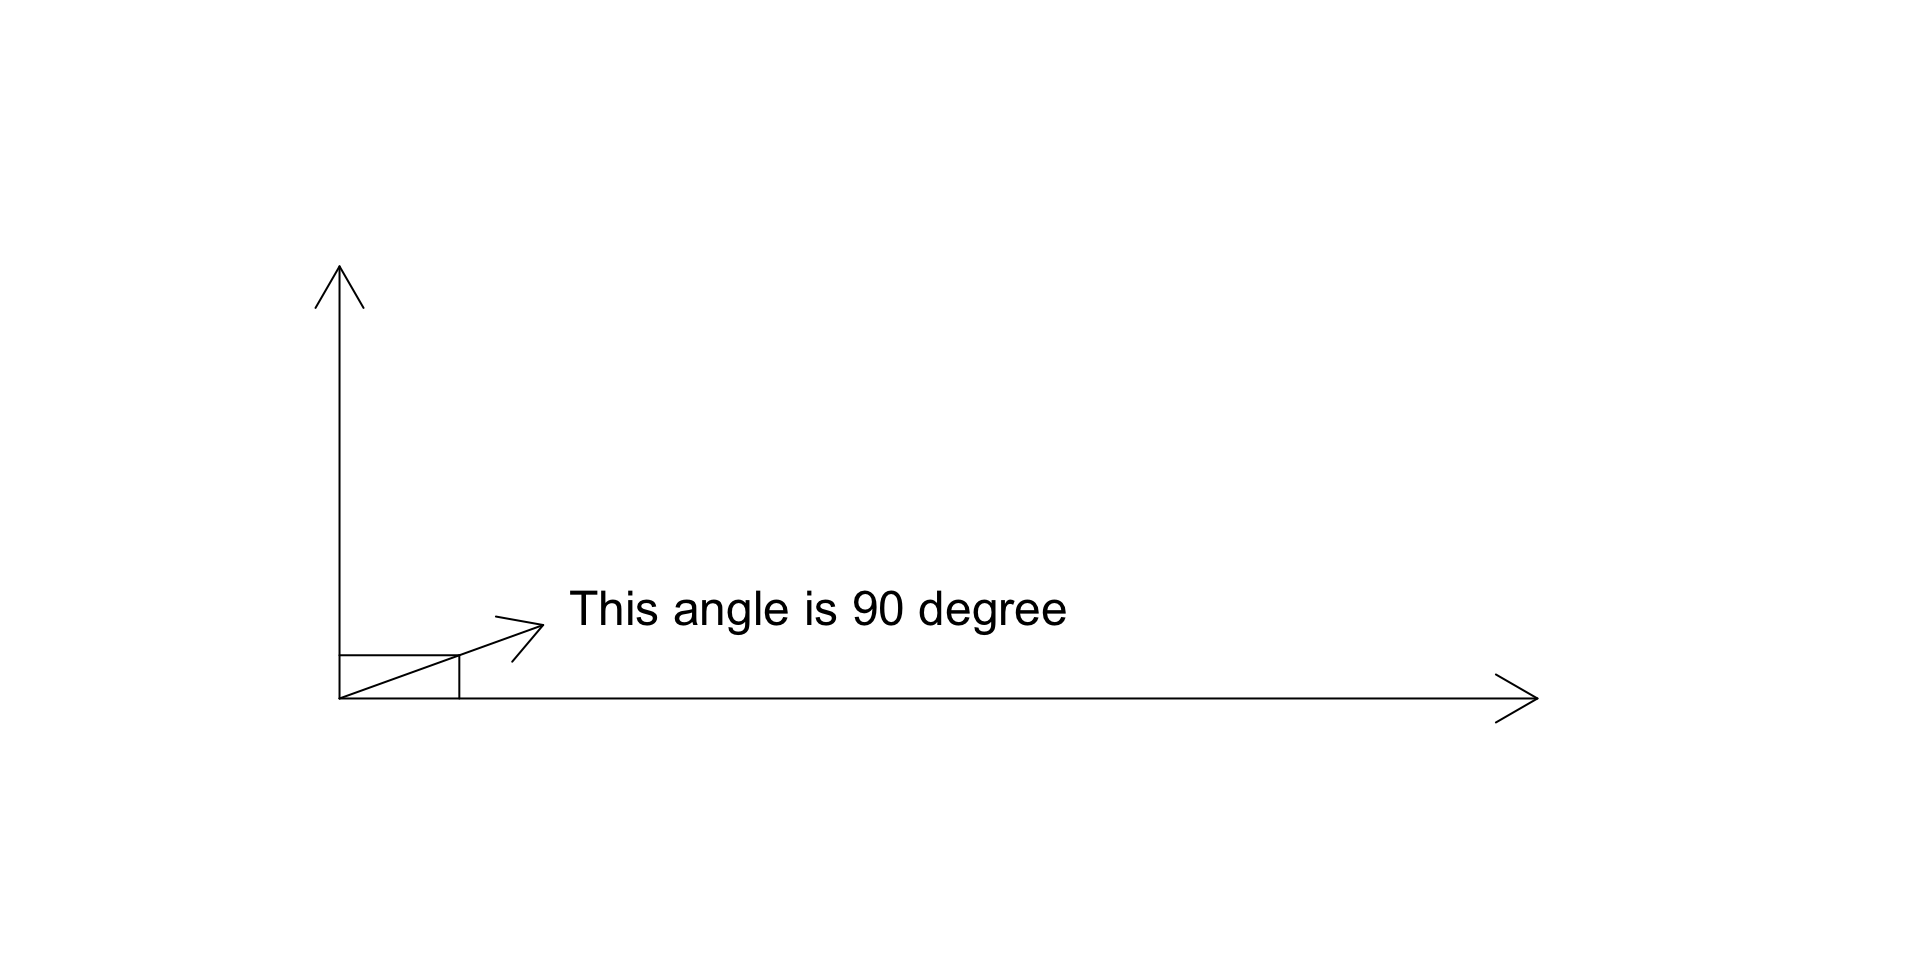
\includegraphics{PCA_files/figure-latex/fig-simple-line4-1} 

}

\caption{We try to fit many lines through the data}\label{fig:fig-simple-line4}
\end{figure}

Figure \ref{fig:fig-simple-line4} shows two arbitrary lines, the lines are called orthogonal/perpendicular to each other.

So now that we know what orthogonal means, we will find a line to be orthogonal to our blue line in Figure \ref{fig:fig-simple-line3}):

\begin{Shaded}
\begin{Highlighting}[]
\CommentTok{# fix number of columns in the plot}
\KeywordTok{par}\NormalTok{(}\DataTypeTok{mfrow=}\KeywordTok{c}\NormalTok{(}\DecValTok{1}\NormalTok{,}\DecValTok{2}\NormalTok{))}
\CommentTok{# define variables}
\NormalTok{var1<-}\DecValTok{18924}
\NormalTok{var3<-}\DecValTok{18505}
\CommentTok{# plot the data}
\KeywordTok{plot}\NormalTok{(data[,}\KeywordTok{c}\NormalTok{(var1,var3)],}\DataTypeTok{xlab =} \StringTok{"Variable 1"}\NormalTok{, }\DataTypeTok{ylab =} \StringTok{"Variable 3"}\NormalTok{,}\DataTypeTok{xlim =} \KeywordTok{c}\NormalTok{(}\DecValTok{2}\NormalTok{,}\DecValTok{15}\NormalTok{),}\DataTypeTok{ylim =} \KeywordTok{c}\NormalTok{(}\DecValTok{2}\NormalTok{,}\DecValTok{15}\NormalTok{))}
\CommentTok{# draw a line}

\CommentTok{# intercept}
\NormalTok{b<-}\OperatorTok{-}\FloatTok{5.172751}
\CommentTok{# slope}
\NormalTok{m<-}\FloatTok{1.548455}
\CommentTok{# draw the line}
\KeywordTok{abline}\NormalTok{(}\DataTypeTok{a =}\NormalTok{ b,}\DataTypeTok{b =}\NormalTok{ m,}\DataTypeTok{col=}\StringTok{"blue"}\NormalTok{,}\DataTypeTok{lwd =} \DecValTok{2}\NormalTok{)}

\CommentTok{# intercept}
\NormalTok{b<-}\FloatTok{11.8710127} 
\CommentTok{# slope}
\NormalTok{m<-}\OperatorTok{-}\FloatTok{0.6458052}
\CommentTok{# draw the line}
\KeywordTok{abline}\NormalTok{(}\DataTypeTok{a =}\NormalTok{ b,}\DataTypeTok{b =}\NormalTok{ m,}\DataTypeTok{col=}\StringTok{"green"}\NormalTok{,}\DataTypeTok{lwd =} \DecValTok{2}\NormalTok{)}



\CommentTok{#}
\NormalTok{projected_variables<-}\KeywordTok{matrix}\NormalTok{(}\OtherTok{NA}\NormalTok{,}\DataTypeTok{nrow =} \KeywordTok{nrow}\NormalTok{(data),}\DataTypeTok{ncol =} \DecValTok{2}\NormalTok{)}
\ControlFlowTok{for}\NormalTok{(i }\ControlFlowTok{in} \DecValTok{1}\OperatorTok{:}\KeywordTok{nrow}\NormalTok{(data))}
\NormalTok{\{}

\CommentTok{# calculate the projection}
\NormalTok{l2 <-}\StringTok{ }\KeywordTok{c}\NormalTok{(}\DecValTok{1}\NormalTok{, m }\OperatorTok{+}\StringTok{ }\NormalTok{b)}
\NormalTok{l1 <-}\StringTok{ }\KeywordTok{c}\NormalTok{(}\DecValTok{0}\NormalTok{, b)}
\NormalTok{l1 <-}\StringTok{ }\KeywordTok{c}\NormalTok{(l1, }\DecValTok{0}\NormalTok{)}
\NormalTok{l2 <-}\StringTok{ }\KeywordTok{c}\NormalTok{(l2, }\DecValTok{0}\NormalTok{)}
\NormalTok{u <-}\StringTok{ }\KeywordTok{sum}\NormalTok{((}\KeywordTok{c}\NormalTok{(data[i,}\KeywordTok{c}\NormalTok{(var1,var3)],}\DecValTok{0}\NormalTok{) }\OperatorTok{-}\StringTok{ }\NormalTok{l1)}\OperatorTok{*}\NormalTok{(l2 }\OperatorTok{-}\StringTok{ }\NormalTok{l1)) }\OperatorTok{/}\StringTok{ }\KeywordTok{sum}\NormalTok{((l2 }\OperatorTok{-}\StringTok{ }\NormalTok{l1)}\OperatorTok{^}\DecValTok{2}\NormalTok{)}
\NormalTok{r<-l1 }\OperatorTok{+}\StringTok{ }\NormalTok{u }\OperatorTok{*}\StringTok{ }\NormalTok{(l2 }\OperatorTok{-}\StringTok{ }\NormalTok{l1)}
\CommentTok{# end projection}

\CommentTok{# draw arrow}
  \KeywordTok{arrows}\NormalTok{(}\DataTypeTok{x0 =}\NormalTok{ data[i,var1],}\DataTypeTok{x1 =}\NormalTok{ r[}\DecValTok{1}\NormalTok{],}
           \DataTypeTok{y0 =}\NormalTok{ data[i,var3],}\DataTypeTok{y1 =}\NormalTok{r[}\DecValTok{2}\NormalTok{],}\DataTypeTok{length=}\FloatTok{0.05}\NormalTok{,}\DataTypeTok{lty=}\StringTok{"dashed"}\NormalTok{)}


\CommentTok{# save the projections}
\NormalTok{projected_variables[i,}\DecValTok{1}\NormalTok{]<-r[}\DecValTok{1}\NormalTok{]}
\NormalTok{projected_variables[i,}\DecValTok{2}\NormalTok{]<-r[}\DecValTok{2}\NormalTok{]}

\NormalTok{\}}


\CommentTok{# plot the data}
\KeywordTok{plot}\NormalTok{(}\DataTypeTok{x=}\NormalTok{decenter_data[,}\DecValTok{2}\NormalTok{],}\DataTypeTok{y=}\KeywordTok{rep}\NormalTok{(}\DecValTok{0}\NormalTok{,}\KeywordTok{nrow}\NormalTok{(data)),}\DataTypeTok{axes =}\NormalTok{ F,}\DataTypeTok{ylab =} \StringTok{""}\NormalTok{,}\DataTypeTok{xlab =} \StringTok{"Combined variable 1 and 3"}\NormalTok{)}
\KeywordTok{axis}\NormalTok{(}\DecValTok{1}\NormalTok{, }\DataTypeTok{col =} \StringTok{'green'}\NormalTok{,}\DataTypeTok{cex=}\DecValTok{4}\NormalTok{,}\DataTypeTok{pos =} \KeywordTok{c}\NormalTok{(}\DecValTok{0}\NormalTok{,}\DecValTok{0}\NormalTok{),}\DataTypeTok{at =}\KeywordTok{unique}\NormalTok{(}\KeywordTok{c}\NormalTok{(}\KeywordTok{floor}\NormalTok{(decenter_data[,}\DecValTok{2}\NormalTok{]),}\KeywordTok{ceiling}\NormalTok{(decenter_data[,}\DecValTok{2}\NormalTok{]))) )}
\end{Highlighting}
\end{Shaded}

\begin{figure}

{\centering 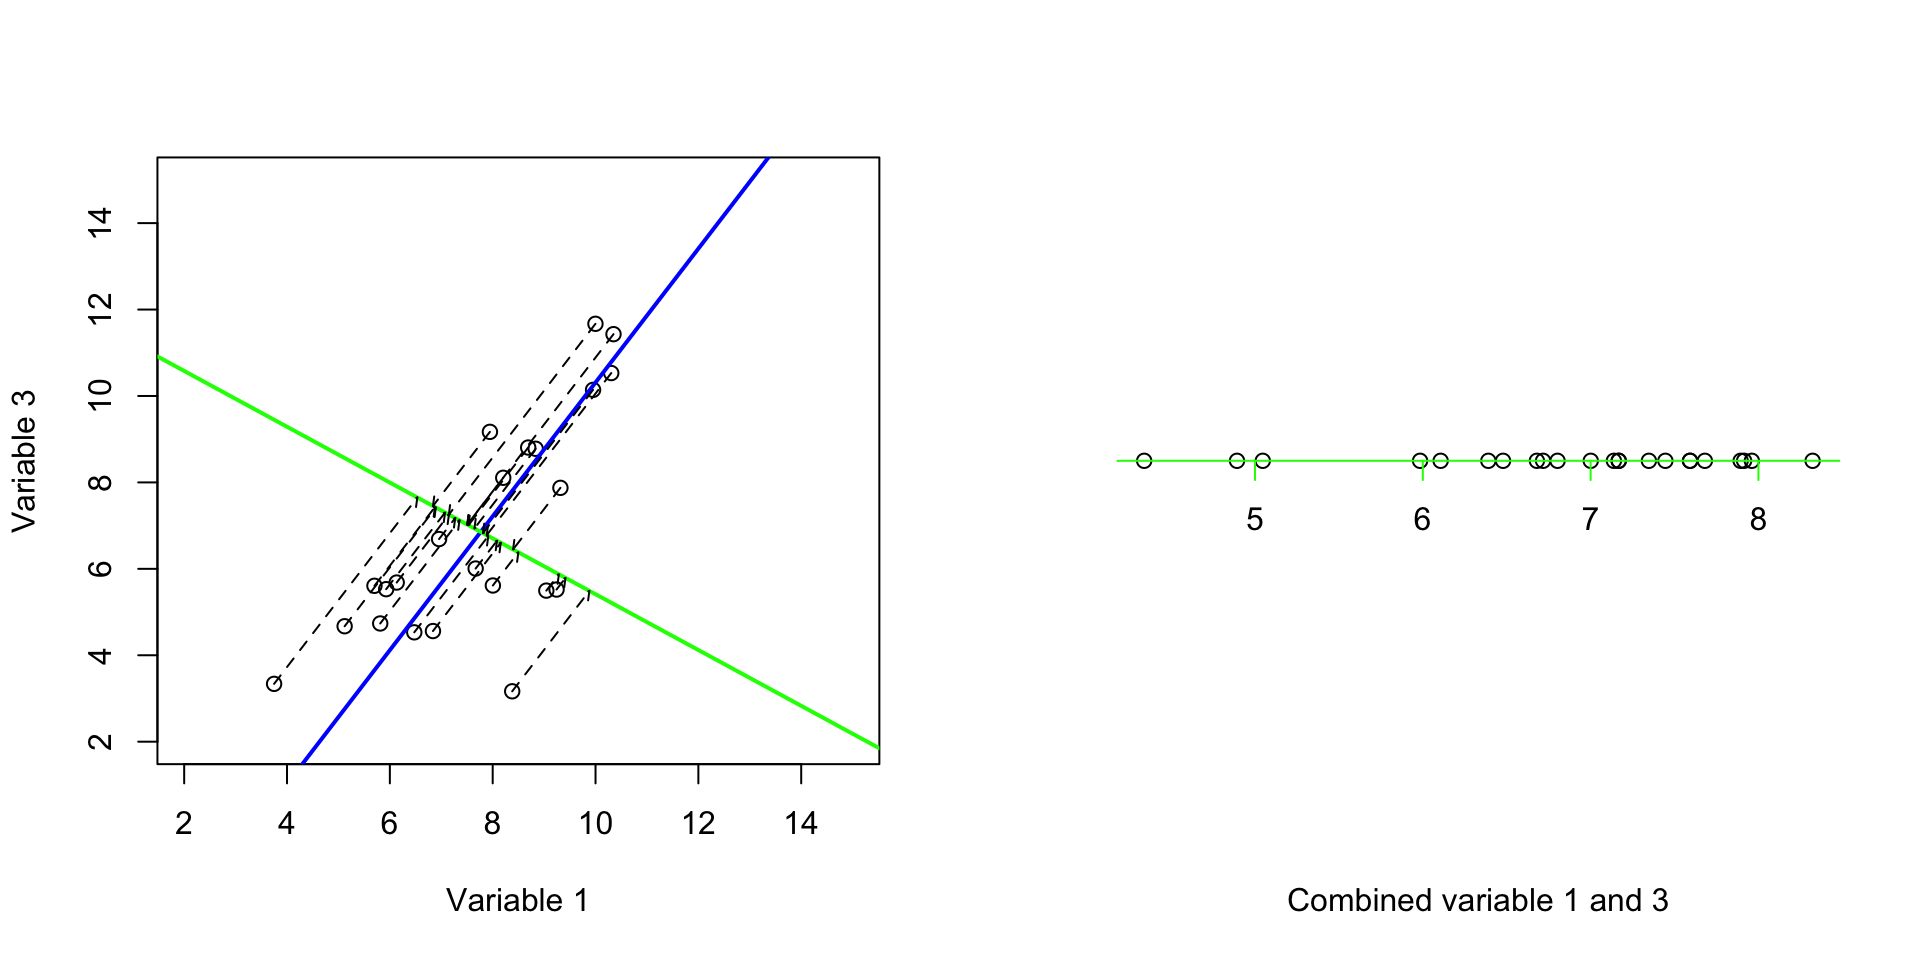
\includegraphics{PCA_files/figure-latex/fig-simple-line5-1} 

}

\caption{We try to fit the second best line through the data}\label{fig:fig-simple-line5}
\end{figure}

Great! Now we have two new axis. The variance of the first one (blue) was 8.5999087 and the second one was 1.0644835. And most importantly, the covariance (redndancy) betweem these two new axis is \ensuremath{3.5564934\times 10^{-10}}. That is almost zero. Perfect! We have two new variables that are showing complementary variation and no redundancy. Please also note that, our small two variable dataset had a total variation of 9.6643921 and our new variables also have 9.6643921. So we did not remove anything! We just rotate the data along two new axis (blue and green) such that our first axis (blue) show us most of the variation and does not have covariance with our second variable. Now it's time to plot both the new variables and see what they show us:

\begin{Shaded}
\begin{Highlighting}[]
\CommentTok{# fix number of columns in the plot}
\KeywordTok{par}\NormalTok{(}\DataTypeTok{mfrow=}\KeywordTok{c}\NormalTok{(}\DecValTok{1}\NormalTok{,}\DecValTok{2}\NormalTok{))}
\CommentTok{# define variables}
\NormalTok{var1<-}\DecValTok{18924}
\NormalTok{var3<-}\DecValTok{18505}
\CommentTok{# plot the data}
\KeywordTok{plot}\NormalTok{(data[,}\KeywordTok{c}\NormalTok{(var1,var3)],}\DataTypeTok{xlab =} \StringTok{"Variable 1"}\NormalTok{, }\DataTypeTok{ylab =} \StringTok{"Variable 3"}\NormalTok{,}\DataTypeTok{col=}\KeywordTok{factor}\NormalTok{(metadata}\OperatorTok{$}\NormalTok{Covariate),}\DataTypeTok{xlim=}\KeywordTok{c}\NormalTok{(}\DecValTok{2}\NormalTok{,}\DecValTok{14}\NormalTok{),}\DataTypeTok{ylim=}\KeywordTok{c}\NormalTok{(}\DecValTok{2}\NormalTok{,}\DecValTok{12}\NormalTok{))}
\KeywordTok{title}\NormalTok{(}\StringTok{"Original variables"}\NormalTok{)}

\CommentTok{# add legend}
\KeywordTok{legend}\NormalTok{(}\StringTok{"topleft"}\NormalTok{, }\DataTypeTok{legend=}\KeywordTok{c}\NormalTok{(}\KeywordTok{unique}\NormalTok{(}\KeywordTok{levels}\NormalTok{(}\KeywordTok{factor}\NormalTok{(metadata}\OperatorTok{$}\NormalTok{Covariate)))),}
       \DataTypeTok{col=}\KeywordTok{unique}\NormalTok{(}\KeywordTok{as.numeric}\NormalTok{(}\KeywordTok{factor}\NormalTok{(metadata}\OperatorTok{$}\NormalTok{Covariate))), }\DataTypeTok{cex=}\FloatTok{0.8}\NormalTok{, }\DataTypeTok{pch =} \DecValTok{1}\NormalTok{)}

\KeywordTok{plot}\NormalTok{(decenter_data,}\DataTypeTok{xlab =} \StringTok{"New variable 1"}\NormalTok{, }\DataTypeTok{ylab =} \StringTok{"New variable 2"}\NormalTok{,}\DataTypeTok{col=}\KeywordTok{factor}\NormalTok{(metadata}\OperatorTok{$}\NormalTok{Covariate),}\DataTypeTok{xlim=}\KeywordTok{c}\NormalTok{(}\DecValTok{2}\NormalTok{,}\DecValTok{14}\NormalTok{),}\DataTypeTok{ylim=}\KeywordTok{c}\NormalTok{(}\DecValTok{2}\NormalTok{,}\DecValTok{12}\NormalTok{),}\DataTypeTok{axes =}\NormalTok{ F)}
\KeywordTok{box}\NormalTok{()}
\KeywordTok{axis}\NormalTok{(}\DecValTok{1}\NormalTok{, }\DataTypeTok{col =} \StringTok{'blue'}\NormalTok{ )}
\KeywordTok{axis}\NormalTok{(}\DecValTok{2}\NormalTok{, }\DataTypeTok{col =} \StringTok{'green'}\NormalTok{ )}

\KeywordTok{title}\NormalTok{(}\StringTok{"New variables"}\NormalTok{)}
\end{Highlighting}
\end{Shaded}

\begin{figure}

{\centering 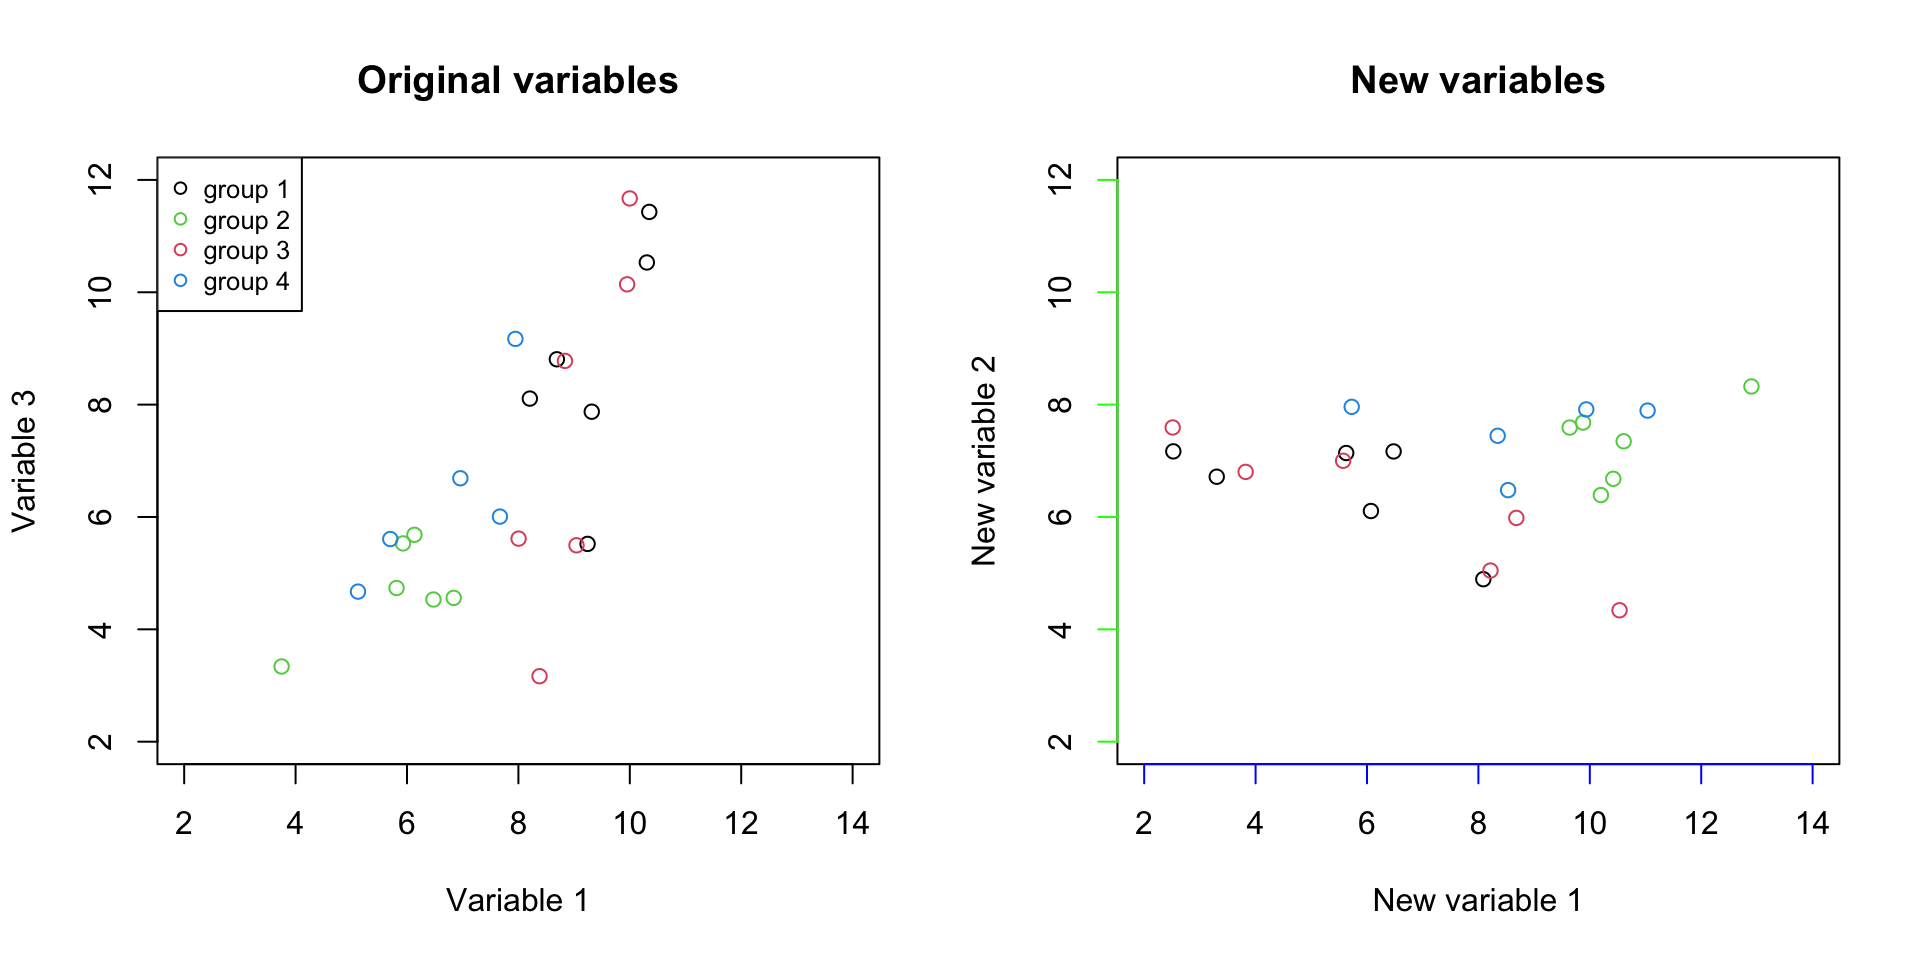
\includegraphics{PCA_files/figure-latex/fig-simple-line6-1} 

}

\caption{Plot of the original variables together with the new axis}\label{fig:fig-simple-line6}
\end{figure}

It should be clear by now that we just rotated the data. But there is one more thing to this \protect\hyperlink{fig-simple-line6}{plot}, in the left, the differences between groups are demonstrated by the values of two variables together (variable 1 and variable 3). However, in the panel on the right, the differences between the groups are mostly visible in just one variable (New variable 1, the blue line). So if we see the variation of interest in one variable, what is the reason to keep the other one? We can simply remove the New variable 2 and represent our data with only one variable.

\begin{Shaded}
\begin{Highlighting}[]
\CommentTok{# fix number of columns in the plot}
\KeywordTok{par}\NormalTok{(}\DataTypeTok{mfrow=}\KeywordTok{c}\NormalTok{(}\DecValTok{1}\NormalTok{,}\DecValTok{1}\NormalTok{))}
\CommentTok{# plot the data}
\KeywordTok{plot}\NormalTok{(}\DataTypeTok{x=}\NormalTok{decenter_data[,}\DecValTok{1}\NormalTok{],}\DataTypeTok{y=}\KeywordTok{rep}\NormalTok{(}\FloatTok{1.2}\NormalTok{,}\KeywordTok{nrow}\NormalTok{(data)),}\DataTypeTok{axes =}\NormalTok{ F,}\DataTypeTok{ylab =} \StringTok{""}\NormalTok{,}\DataTypeTok{xlab =} \StringTok{"New variable 1"}\NormalTok{,}\DataTypeTok{col=}\KeywordTok{factor}\NormalTok{(metadata}\OperatorTok{$}\NormalTok{Covariate))}
\KeywordTok{axis}\NormalTok{(}\DecValTok{1}\NormalTok{, }\DataTypeTok{col =} \StringTok{'blue'}\NormalTok{,}\DataTypeTok{cex=}\DecValTok{4}\NormalTok{,}\DataTypeTok{pos=}\KeywordTok{c}\NormalTok{(}\DecValTok{1}\NormalTok{,}\DecValTok{1}\NormalTok{),}\DataTypeTok{at =}\KeywordTok{unique}\NormalTok{(}\KeywordTok{c}\NormalTok{(}\KeywordTok{floor}\NormalTok{(decenter_data[,}\DecValTok{1}\NormalTok{]),}\KeywordTok{ceiling}\NormalTok{(decenter_data[,}\DecValTok{1}\NormalTok{]))) )}

\CommentTok{# add legend}
\KeywordTok{legend}\NormalTok{(}\StringTok{"topleft"}\NormalTok{, }\DataTypeTok{legend=}\KeywordTok{c}\NormalTok{(}\KeywordTok{unique}\NormalTok{(}\KeywordTok{levels}\NormalTok{(}\KeywordTok{factor}\NormalTok{(metadata}\OperatorTok{$}\NormalTok{Covariate)))),}
       \DataTypeTok{col=}\KeywordTok{unique}\NormalTok{(}\KeywordTok{as.numeric}\NormalTok{(}\KeywordTok{factor}\NormalTok{(metadata}\OperatorTok{$}\NormalTok{Covariate))), }\DataTypeTok{cex=}\FloatTok{0.8}\NormalTok{, }\DataTypeTok{pch =} \DecValTok{1}\NormalTok{)}
\end{Highlighting}
\end{Shaded}

\begin{figure}

{\centering 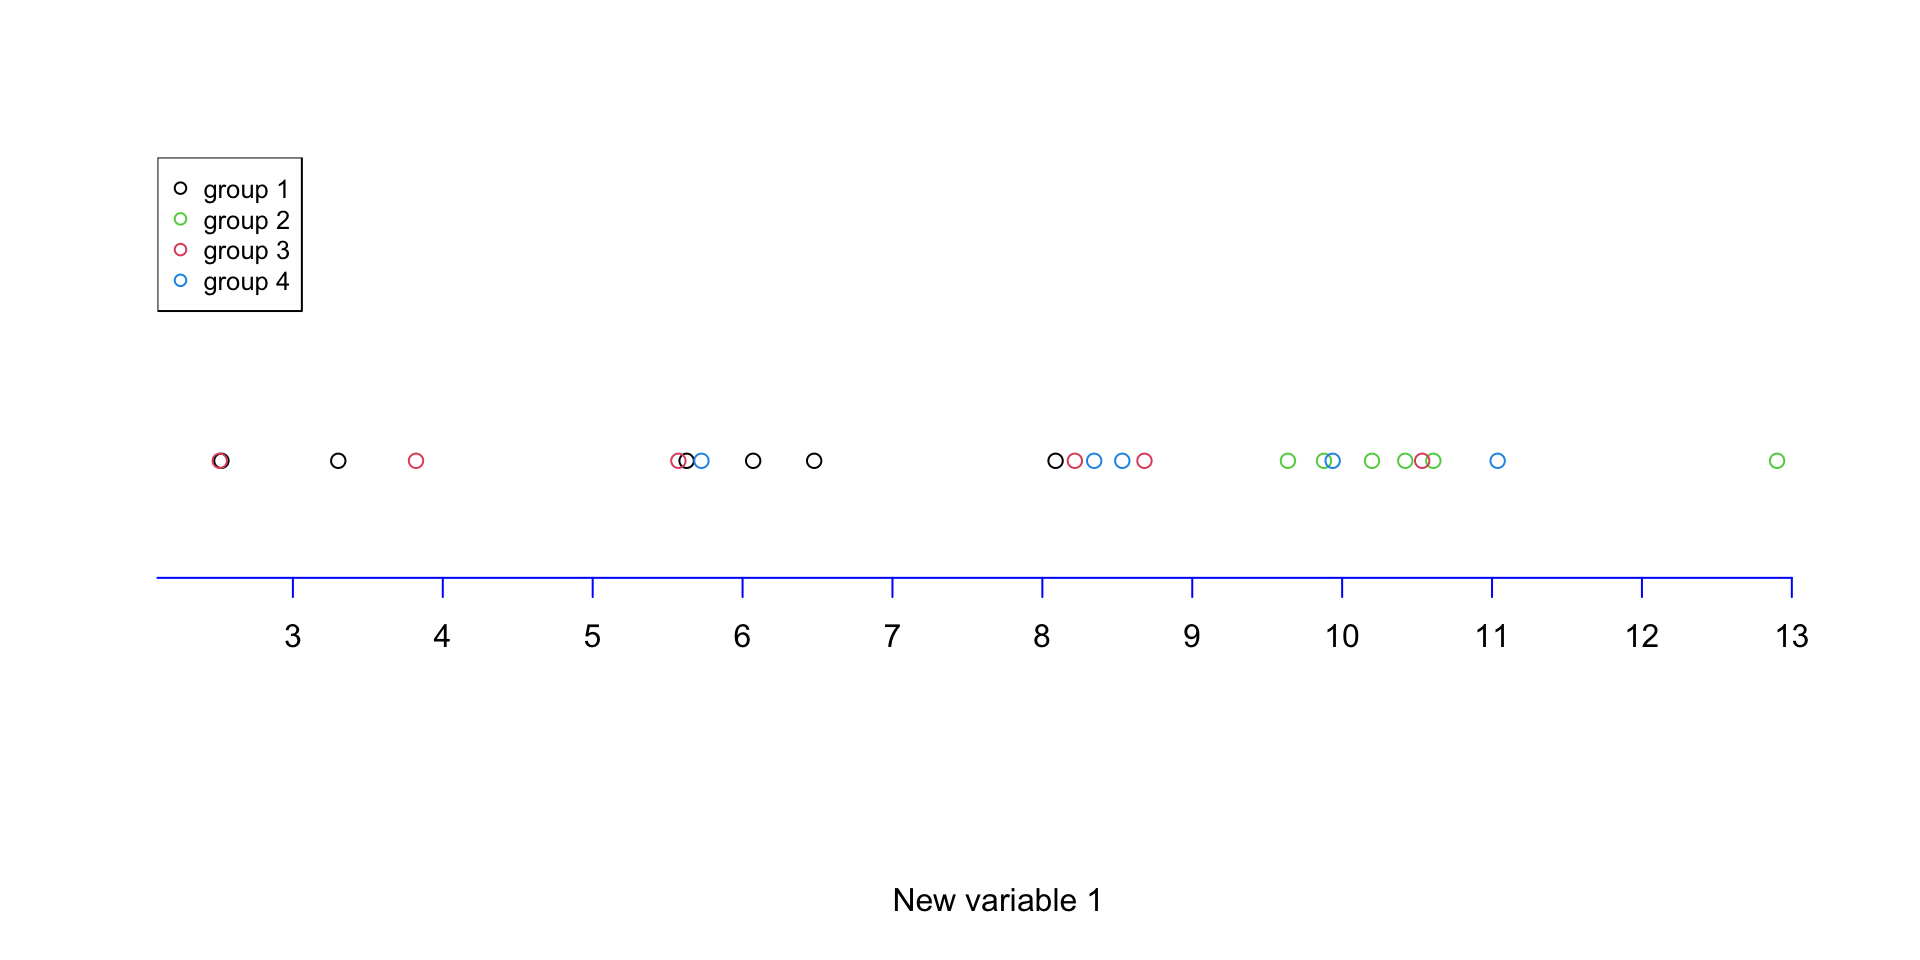
\includegraphics{PCA_files/figure-latex/fig-remove1-1} 

}

\caption{Plot of the data with one of the variables removed}\label{fig:fig-remove1}
\end{figure}

We can see in Figure \ref{fig:fig-remove1} that the differences are represented in one variable what is the combined effect of the two original variables. This might not sound such a big deal as one of our original variables (Variable 1) already represented the data very well. In addition, when removing the new variable 2, in fact we only remove 11 percent of the variation. Whereas if we remove either of the original variable 1 or 2, we will remove 34 or 66 percent respectively. Meaning that using the aforementioned method, we concentrated the variation in a limited number of variables. So removing the variable with little variation should not harm the overal data pattern. Reducing from two variables to one is not such a big deal! But how about reducing from 45101 variables to just a few ones? This is exactly what PCA does!

\hypertarget{pcafri}{%
\section{PCA (freindly definition)}\label{pcafri}}

PCA does exactly what we have been doing so far but it can do it for much much more complex data with thousands of variables (e.g.~genes)! Its job is to find new variables from the combination of original variables and then sort them. It does that in a way that, after sorting, the first variable has the most variation (e.g.~information), the second one has the second most and so forth. And all this amazing thing comes with the luxury of not having redundant variation between the new variables.

All these words mean that PCA will take your data, and rotate them and show you the angle of the data that you will see most of the differences between your observations (e.g.~samples/patients/data points etc). It does this unbiased, without knowing what you are interested in. It simply does not care! For PCA higher variation is better, it will simply show it first. That is exactly the reason why it's a fantastic method for finding hidden pattern in the data. We will go through a few examples in \protect\hyperlink{pcaapplications}{the next chapter}.

In short, you can do the following with PCA:

\begin{itemize}
\tightlist
\item
  \protect\hyperlink{pcavisdimreduct}{Visualization of high dimensional data}: dimensions are normally the number of variables (e.g.~genes) that are in the dataset
\item
  \protect\hyperlink{pcavisdimreduct}{Dimentionality reduction}: exactly like we did here for removing variables
\item
  \protect\hyperlink{pcavarselect}{Variable selection}: selecting which of the variables (e.g.~genes) has most influence on the overal data pattern
\item
  \protect\hyperlink{pcabtrm}{Batch removing}: Batch effect or other experimental biases can be removed by PCA
\end{itemize}

We are going to go through all the abovementinoed points in the next chapter.

See you!

\hypertarget{pcaapplications}{%
\chapter{PCA (applications)}\label{pcaapplications}}

\hypertarget{summary-of-the-previous-chapter-1}{%
\section{Summary of the previous chapter}\label{summary-of-the-previous-chapter-1}}

We have \protect\hyperlink{pcafri}{already discussed} what PCA does. This method is used to create a set of new variables that are combination of the original variables. PCA then sort these variables in descending order with respect to their variation. The total variation of all new variables are always the same as the original ones. The new variables will be always orthogonal (no covariance, no redundancy). Simply talking, PCA rotates the data and shows a particular view of the data such that the user can see where most of the variation is sitting! One can later decide where this variation is of interest or not depending on the research question. At this stage, we would like to remind you about the dataset we are using. In our data we have 23 observations (e.g.~samples/patients) and 45101 variables (e.g.~measurements such as genes). The observation are coming from 4 groups: group 1, group 2, group 3, group 4 (e.g.~cancer sub-types). We have been coloring our points in the plot based on these groups. Finally this experiment was run in 2 batches (in the lab!). So let's get started by doing some PCA!

\hypertarget{pcar}{%
\section{PCA in R}\label{pcar}}

We are going to use \emph{prcomp} function in R to perform PCA. The main reason for selecting this function is simple. This is a function that is coming default with R, gives decent accuracy and is more or less accepted at the default method of doing a PCA in R. However, you should note that there are many more ways of doing a PCA in R, some of which provide much more functionalities compared to \emph{prcomp}.

Before proceeding with using \emph{prcomp}, it is important to organize your data correctly:

\begin{itemize}
\tightlist
\item
  From now on, your data is a matrix (like table! although it's sloppy to say that!)
\item
  \textbf{Your observations (e.g.~samples) are in rows}
\item
  \textbf{Your variables (e.g.~measurements) are in column}
\end{itemize}

\emph{If you ever wanted to use other functions, please do check in what format they need the data. This is important}

So to give you an example, we show you part of our data:

\begin{Shaded}
\begin{Highlighting}[]
\CommentTok{# show 10 variables and all the samples}
\NormalTok{knitr}\OperatorTok{::}\KeywordTok{kable}\NormalTok{(}\KeywordTok{as.data.frame}\NormalTok{(}\KeywordTok{round}\NormalTok{(data[,}\DecValTok{1}\OperatorTok{:}\DecValTok{5}\NormalTok{],}\DecValTok{2}\NormalTok{)),}\DataTypeTok{caption =} \StringTok{"An example matrix where samples are in the rows and variables are in column"}\NormalTok{)}
\end{Highlighting}
\end{Shaded}

\begin{table}

\caption{\label{tab:tablesample}An example matrix where samples are in the rows and variables are in column}
\centering
\begin{tabular}[t]{l|r|r|r|r|r}
\hline
  & V1 & V2 & V3 & V4 & V5\\
\hline
Sample1\_Group1\_Batch1 & 1.67 & 1.85 & 1.53 & 1.39 & 1.83\\
\hline
Sample2\_Group1\_Batch1 & 1.44 & 1.71 & 1.76 & 1.53 & 2.06\\
\hline
Sample3\_Group1\_Batch1 & 1.33 & 1.77 & 1.76 & 1.53 & 1.76\\
\hline
Sample4\_Group1\_Batch1 & 1.54 & 1.95 & 1.73 & 1.48 & 1.76\\
\hline
Sample5\_Group3\_Batch1 & 1.52 & 1.88 & 1.63 & 1.40 & 1.73\\
\hline
Sample6\_Group3\_Batch1 & 1.76 & 1.65 & 1.82 & 1.53 & 1.74\\
\hline
Sample7\_Group3\_Batch1 & 1.63 & 1.77 & 1.84 & 1.48 & 1.88\\
\hline
Sample8\_Group3\_Batch1 & 1.59 & 1.65 & 1.63 & 1.58 & 1.69\\
\hline
Sample9\_Group3\_Batch1 & 1.41 & 1.67 & 1.65 & 1.49 & 1.76\\
\hline
Sample10\_Group2\_Batch1 & 1.54 & 1.77 & 1.53 & 1.48 & 1.63\\
\hline
Sample11\_Group2\_Batch1 & 1.57 & 2.17 & 1.53 & 1.47 & 1.76\\
\hline
Sample12\_Group2\_Batch1 & 1.47 & 1.79 & 1.83 & 1.47 & 1.56\\
\hline
Sample13\_Group2\_Batch1 & 1.53 & 1.49 & 1.43 & 1.37 & 1.78\\
\hline
Sample14\_Group4\_Batch1 & 1.50 & 1.74 & 1.58 & 1.50 & 1.77\\
\hline
Sample15\_Group4\_Batch1 & 1.70 & 1.98 & 1.48 & 1.56 & 1.82\\
\hline
Sample16\_Group1\_Batch2 & 2.17 & 2.49 & 2.40 & 2.28 & 2.54\\
\hline
Sample4\_Group1\_Batch2 & 2.08 & 2.55 & 2.25 & 2.09 & 2.55\\
\hline
SampleA\_Group2\_Batch2 & 2.28 & 2.71 & 2.44 & 2.26 & 2.35\\
\hline
Sample10\_Group2\_Batch2 & 2.28 & 2.50 & 2.18 & 2.17 & 2.34\\
\hline
Sample5\_Group3\_Batch2 & 2.20 & 2.48 & 2.27 & 2.17 & 2.33\\
\hline
SampleB\_Group4\_Batch2 & 2.08 & 2.38 & 2.44 & 2.21 & 2.36\\
\hline
SampleCGroup4\_Batch2 & 2.02 & 2.31 & 2.20 & 2.16 & 2.43\\
\hline
SampleD\_Group4\_Batch2 & 1.89 & 2.10 & 2.11 & 2.14 & 2.14\\
\hline
\end{tabular}
\end{table}

As you see in Table \ref{tab:tablesample}, the observations are in rows (e.g.~Sample1\_Group1\_Batch1) and variables are in columns (e.g.~V1).

By now you should now how to use functions in R. However, for just a brief reminder, a function is like a small program and does something. Exactly like in Microsoft Word where you click on some menus to for example to change the font. You then need to select the font, style, size etc. These options, we tend to call them parameters or arguments. Normally functions in R need a few parameters in order to do exactly what you want. \emph{prcomp} is no exception! Fortunately, the number of parameters that we will use is not too many:

\begin{itemize}
\tightlist
\item
  x: is your data matrix
\item
  center: Shifts the variables to have zero mean (Don't panic! See below)
\item
  scale: Scales the variables to have unit variance (Scary huh?! See below)
\end{itemize}

That was it. We won't use the rest of the parameters! You actually don't need them unless you are doing something very special!

The way that we run a function in R is to write name of the function then parenthesis open, add parameters (separated by comma) and parenthesis close! So for running a PCA we can do for example:

\begin{verbatim}
prcomp(x=x,center=TRUE,scale. = TRUE)
\end{verbatim}

This is normally reffered to as \emph{calling a function}. It says, run a pca, with parameters, x equals to x, center is true and scale is also true. Many functions in R give the results of their jobs some form. We normally say, they return something. So we can even be cooler and save the retuned results somewhere so we can use it.

\begin{verbatim}
pcaResults <- prcomp(x=x,center=TRUE,scale. = TRUE)
\end{verbatim}

As said before, \emph{x} is your data matrix that we have already \protect\hyperlink{tablesample}{prepared}.

\hypertarget{centering}{%
\section{Centering}\label{centering}}

We have a set of variables (e.g genes) in our data. If we set centering to \emph{TRUE}, R, first, will calculate average of each variable and then subtract this average from the values of the variable (for each observation, e.g.~sample).

In short, it will shift the data so that the center of our data is zero. We can see an example of this for ten of our variables:

\begin{Shaded}
\begin{Highlighting}[]
\CommentTok{# set number of figures}
\KeywordTok{par}\NormalTok{(}\DataTypeTok{mfrow=}\KeywordTok{c}\NormalTok{(}\DecValTok{1}\NormalTok{,}\DecValTok{2}\NormalTok{))}
\CommentTok{# show 10 variables and all the samples}
\KeywordTok{boxplot}\NormalTok{(data[,}\DecValTok{1}\OperatorTok{:}\DecValTok{10}\NormalTok{],}\DataTypeTok{xlab=}\StringTok{"Variable"}\NormalTok{,}\DataTypeTok{ylab=}\StringTok{"Variable value (e.g. expression)"}\NormalTok{)}
\KeywordTok{title}\NormalTok{(}\StringTok{"Original data"}\NormalTok{)}
\CommentTok{# calculate the means}
\NormalTok{means <-}\StringTok{ }\KeywordTok{apply}\NormalTok{(data[,}\DecValTok{1}\OperatorTok{:}\DecValTok{10}\NormalTok{],}\DecValTok{2}\NormalTok{,mean)}
\CommentTok{#plot the means}
\KeywordTok{points}\NormalTok{(}\DataTypeTok{x=}\DecValTok{1}\OperatorTok{:}\DecValTok{10}\NormalTok{,}\DataTypeTok{y =}\NormalTok{ means,}\DataTypeTok{col=}\StringTok{"red"}\NormalTok{,}\DataTypeTok{pch=}\DecValTok{18}\NormalTok{)}


\CommentTok{# show 10 variables and all the samples but centered}
\KeywordTok{boxplot}\NormalTok{(}\KeywordTok{scale}\NormalTok{(data[,}\DecValTok{1}\OperatorTok{:}\DecValTok{10}\NormalTok{],}\DataTypeTok{center =} \OtherTok{TRUE}\NormalTok{, }\DataTypeTok{scale =} \OtherTok{FALSE}\NormalTok{),}\DataTypeTok{xlab=}\StringTok{"Variable"}\NormalTok{,}
        \DataTypeTok{ylab=}\StringTok{"Variable value (e.g. expression)"}\NormalTok{)}
\KeywordTok{title}\NormalTok{(}\StringTok{"Centered data"}\NormalTok{)}
\CommentTok{# calculate the means}
\NormalTok{means <-}\StringTok{ }\KeywordTok{apply}\NormalTok{(}\KeywordTok{scale}\NormalTok{(data[,}\DecValTok{1}\OperatorTok{:}\DecValTok{10}\NormalTok{],}\DataTypeTok{center =} \OtherTok{TRUE}\NormalTok{, }\DataTypeTok{scale =} \OtherTok{FALSE}\NormalTok{),}\DecValTok{2}\NormalTok{,mean)}
\CommentTok{#plot the means}
\KeywordTok{points}\NormalTok{(}\DataTypeTok{x=}\DecValTok{1}\OperatorTok{:}\DecValTok{10}\NormalTok{,}\DataTypeTok{y =}\NormalTok{ means,}\DataTypeTok{col=}\StringTok{"red"}\NormalTok{,}\DataTypeTok{pch=}\DecValTok{18}\NormalTok{)}
\end{Highlighting}
\end{Shaded}

\begin{figure}

{\centering 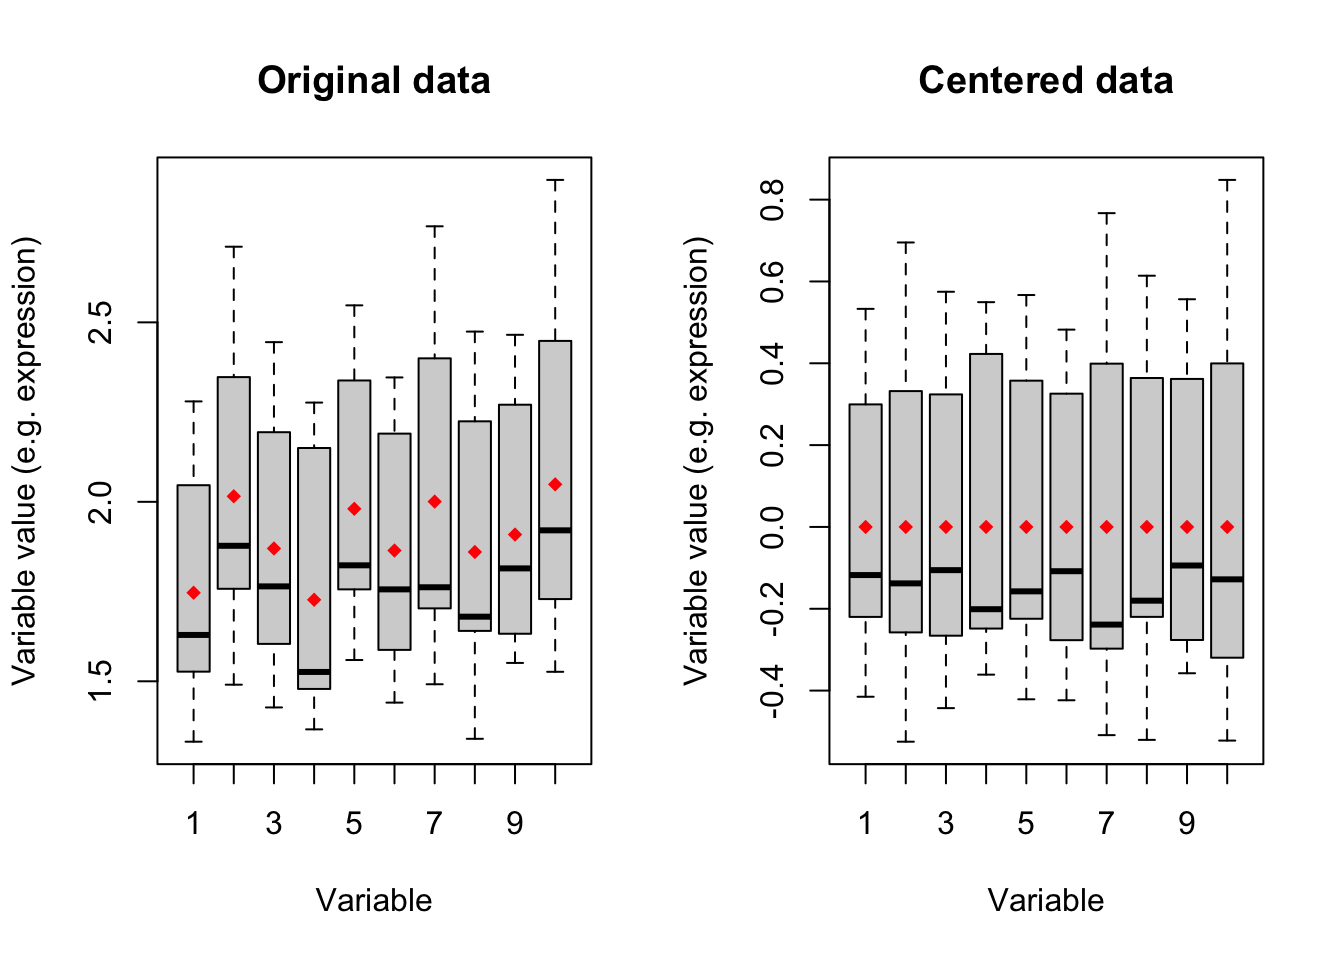
\includegraphics{PCA_files/figure-latex/centerExample-1} 

}

\caption{Boxplot of ten variables before and after centering}\label{fig:centerExample}
\end{figure}

Figure \ref{fig:centerExample} shows boxplots of ten variables in our data. The left panel is showing the original data where the mean of each variable has been showing in red dimonds. In the right panel, we see that after centering the mean of all variables become zero. We will go through this in detail later. for now:

\textbf{IMPORTANT: You MUST center your data for doing PCA. If your data is not centered, you are NOT doing PCA.}

Setting the \emph{center} parameters to \emph{TRUE} will force prcomp to center your data automatically. \textbf{DO NOT set this to FALSE if you are not sure whether your data is centered}

\hypertarget{scaling}{%
\section{Scaling}\label{scaling}}

Many datasets typically come in different scales and this happens even within a dataset. That means that if i measures three variables (e.g genes), the scale of the measurements can be different between these three. This is specially the case for high throughput experiments where thousands of variables are measured at the same time. A mini example would be one person measuring height in centimeter and another one measuring height in meter. Scaling is a way of forcing your variables to show one unit scale. One common of way of doing this, is to calculate standard deviation (square root of variance) of each variable, and divide the variable by this standard deviation. Let's see if we can demonstrate what it means with an example:

\begin{Shaded}
\begin{Highlighting}[]
\CommentTok{# set number of figures}
\KeywordTok{par}\NormalTok{(}\DataTypeTok{mfrow=}\KeywordTok{c}\NormalTok{(}\DecValTok{1}\NormalTok{,}\DecValTok{2}\NormalTok{))}

\CommentTok{# create two variables}
\NormalTok{varibale1<-data[,var1]}
\NormalTok{varibale2<-data[,var1]}\OperatorTok{*}\DecValTok{10}

\CommentTok{# create a data frame}
\NormalTok{dataDummy<-}\KeywordTok{data.frame}\NormalTok{(}\DataTypeTok{Variable1=}\NormalTok{varibale1,}\DataTypeTok{Variable2=}\NormalTok{varibale2)}


\CommentTok{# show 10 variables and all the samples}
\KeywordTok{boxplot}\NormalTok{(dataDummy,}\DataTypeTok{xlab=}\StringTok{"Variable"}\NormalTok{,}\DataTypeTok{ylab=}\StringTok{"Variable value (e.g. expression)"}\NormalTok{)}

\CommentTok{# plot scatter}
\KeywordTok{plot}\NormalTok{(dataDummy)}
\end{Highlighting}
\end{Shaded}

\begin{figure}

{\centering 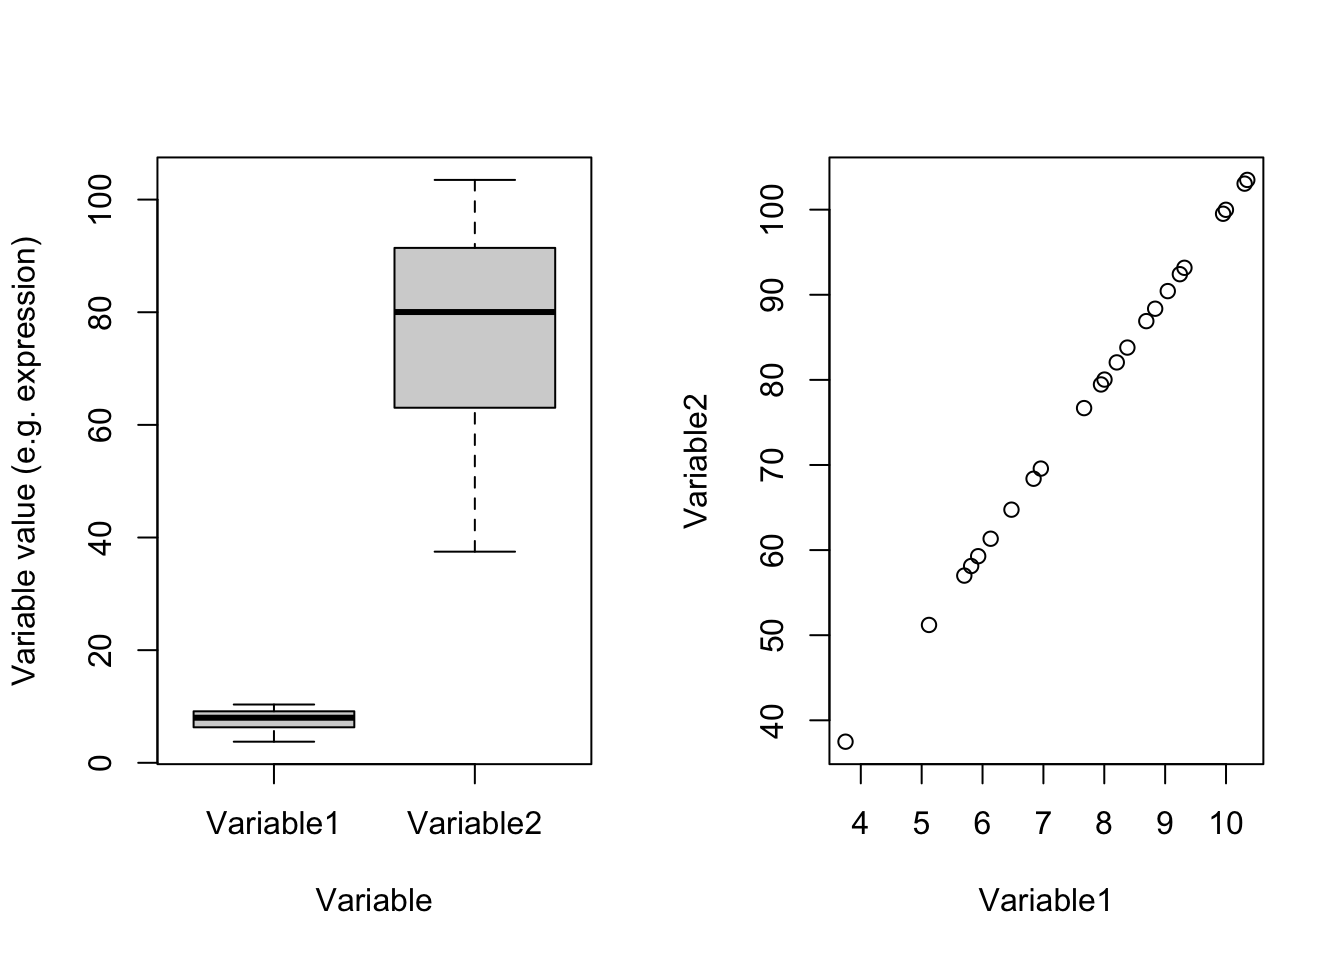
\includegraphics{PCA_files/figure-latex/scaleExample1-1} 

}

\caption{Example of two variables with different scales}\label{fig:scaleExample1}
\end{figure}

In Figure \ref{fig:scaleExample1}(left panel) which one of these two variables has most of the variation? Well you are right! Variable2 has 328.2277629 whereas Variable1 has 3.2822776. Remember what PCA shows: the angle with most of the variation. Obviously, this is going to be Variable2. There is one point and i guess you also see it in the code. These two variables are identical except that Variable2 equals to Variable1 multiply by 100. You can see that in the scatter plot in the right panel. These two variables are identical. Let's see the effect of scalling:

\begin{Shaded}
\begin{Highlighting}[]
\CommentTok{# set number of figures}
\KeywordTok{par}\NormalTok{(}\DataTypeTok{mfrow=}\KeywordTok{c}\NormalTok{(}\DecValTok{1}\NormalTok{,}\DecValTok{2}\NormalTok{))}

\CommentTok{# create two variables}
\NormalTok{varibale1<-data[,var1]}
\NormalTok{varibale2<-data[,var1]}\OperatorTok{*}\DecValTok{10}

\CommentTok{# create a data frame}
\NormalTok{dataDummy<-}\KeywordTok{data.frame}\NormalTok{(}\DataTypeTok{Variable1=}\NormalTok{varibale1,}\DataTypeTok{Variable2=}\NormalTok{varibale2)}

\CommentTok{# scale the data, not center}
\NormalTok{dataDummy<-}\KeywordTok{scale}\NormalTok{(dataDummy,}\DataTypeTok{center =} \OtherTok{FALSE}\NormalTok{, }\DataTypeTok{scale =} \OtherTok{TRUE}\NormalTok{)}

\CommentTok{# show 10 variables and all the samples}
\KeywordTok{boxplot}\NormalTok{(dataDummy,}\DataTypeTok{xlab=}\StringTok{"Variable"}\NormalTok{,}\DataTypeTok{ylab=}\StringTok{"Variable value (e.g. expression)"}\NormalTok{)}

\CommentTok{# plot scatter}
\KeywordTok{plot}\NormalTok{(dataDummy)}
\end{Highlighting}
\end{Shaded}

\begin{figure}

{\centering 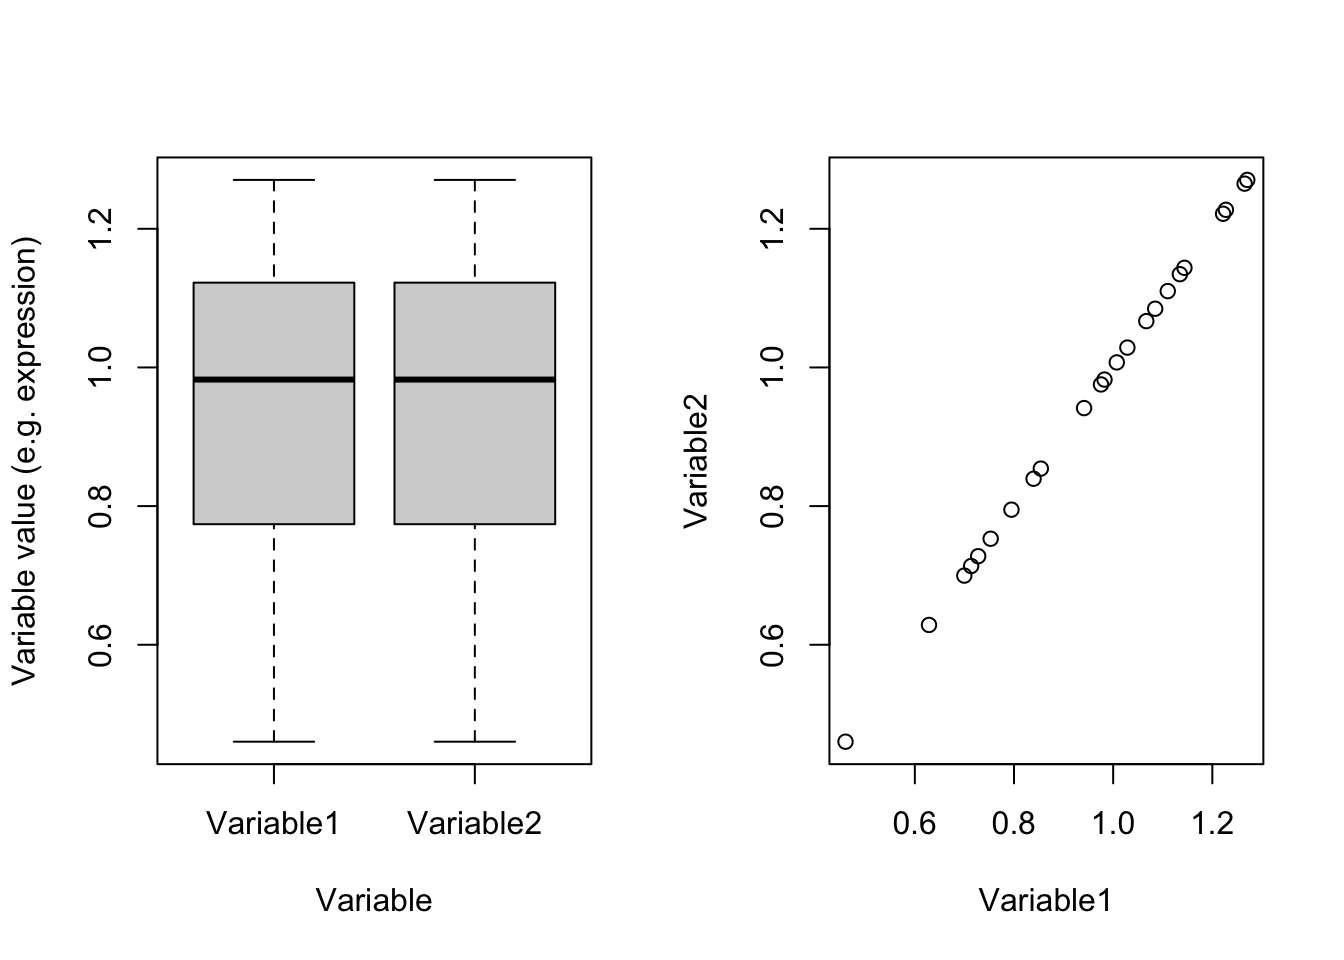
\includegraphics{PCA_files/figure-latex/scaleExample2-1} 

}

\caption{Example of two variables which are scalled}\label{fig:scaleExample2}
\end{figure}

Perfect! right?! Now we see that they are identical and obviously have the same variation (0.0494634). So we were fooled by scales. If we have thousands of variables and just one or two of them are coming from a different scales compared to the rest, PCA would also have been fooled and showed us only those two variables! So the point is:

\textbf{If you don't know your variables are in the same scale, set \emph{scale} to \emph{TRUE}}

The rule of thumb is that, if you don't know anything about your data, set both scale and center to TRUE. You will be probably safe :)

Now it's time to use PCA to do something.

\begin{Shaded}
\begin{Highlighting}[]
\CommentTok{# do pca}
\NormalTok{pcaResults<-}\KeywordTok{prcomp}\NormalTok{(data,}\DataTypeTok{scale. =}\NormalTok{ T,}\DataTypeTok{center =}\NormalTok{ T)}

\CommentTok{# convert pca result to dataframe}
\NormalTok{pcaResults_table<-}\KeywordTok{data.frame}\NormalTok{(}\DataTypeTok{Elements =} \KeywordTok{names}\NormalTok{(pcaResults),}
           \DataTypeTok{Classes =} \KeywordTok{sapply}\NormalTok{(pcaResults, }\ControlFlowTok{function}\NormalTok{(x)}\KeywordTok{class}\NormalTok{(x)[}\DecValTok{1}\NormalTok{]),}
           \DataTypeTok{row.names =} \KeywordTok{c}\NormalTok{(}\DecValTok{2}\NormalTok{,}\DecValTok{3}\NormalTok{,}\DecValTok{4}\NormalTok{,}\DecValTok{5}\NormalTok{,}\DecValTok{1}\NormalTok{))}

\CommentTok{# make a table}
\NormalTok{knitr}\OperatorTok{::}\KeywordTok{kable}\NormalTok{(pcaResults_table[}\KeywordTok{order}\NormalTok{(}\KeywordTok{rownames}\NormalTok{(pcaResults_table)),],}\DataTypeTok{caption =} \StringTok{"PCA output classes"}\NormalTok{)}
\end{Highlighting}
\end{Shaded}

\begin{table}

\caption{\label{tab:tabpca1}PCA output classes}
\centering
\begin{tabular}[t]{l|l}
\hline
Elements & Classes\\
\hline
x & matrix\\
\hline
sdev & numeric\\
\hline
rotation & matrix\\
\hline
center & numeric\\
\hline
scale & numeric\\
\hline
\end{tabular}
\end{table}

PCA gives you a list. A list in R can be thought of a database that keep many different type of information for you (called elements). You can see what type of information is in the result (list) of PCA in table \ref{tab:tabpca1}. The single elemnts of PCA list can be accessed using the dollar sign (\emph{\$}) which comes immediately after the name of the list.

For example if you want to see the values of x, it can be accessed by

\begin{verbatim}
pcaResults$x
\end{verbatim}

Or rotations can be accessed by

\begin{verbatim}
pcaResults$rotation
\end{verbatim}

In the next sections we will use these elements to investigate our data.

\hypertarget{pcavisdimreduct}{%
\section{Visualization of data and dimentionality reduction}\label{pcavisdimreduct}}

One of primary aspect of pattern recognition is to visually look at the data and see how the observations (samples) have been spread compared to each other. Do we see our treatment to be well separated from our control groups (potentially indicating a treatment effect)? Do we see a gradient of sample spread with respect to dose of a drug we gave to the patients? Do we have any unnoticed experimental bias? The list of questions can go on and on and it's pretty much impossible to list them all. The key point here is that for the reasons that we previously mentioned, it's difficult ot look at the original data mainly due to large number of variables and in addition maybe the effect of interest is not ``caused'' by one variable but a combinition of different variables. We can use PCA (or similar methods) to squeeze the data into a set of limited variables that is easier to look at.

These new variables are in \emph{x} element of our pca result. These are normally called PC scores or \emph{variates} or \emph{x}.

Let's have a look at this:

\begin{Shaded}
\begin{Highlighting}[]
\CommentTok{# make a table}
\NormalTok{knitr}\OperatorTok{::}\KeywordTok{kable}\NormalTok{(pcaResults}\OperatorTok{$}\NormalTok{x[,}\DecValTok{1}\OperatorTok{:}\DecValTok{5}\NormalTok{],}
      \DataTypeTok{caption =} \StringTok{"PCA output Scores (only top 5 are shown)"}\NormalTok{)}
\end{Highlighting}
\end{Shaded}

\begin{table}

\caption{\label{tab:tabpca2}PCA output Scores (only top 5 are shown)}
\centering
\begin{tabular}[t]{l|r|r|r|r|r}
\hline
  & PC1 & PC2 & PC3 & PC4 & PC5\\
\hline
Sample1\_Group1\_Batch1 & -142.4977 & -20.151157 & 7.364239 & -23.7018049 & 4.9708775\\
\hline
Sample2\_Group1\_Batch1 & -135.2110 & -50.462934 & 43.692008 & -4.1229620 & -1.9423228\\
\hline
Sample3\_Group1\_Batch1 & -139.0443 & -61.125761 & -4.613422 & 38.4579480 & -22.1566490\\
\hline
Sample4\_Group1\_Batch1 & -140.9501 & 8.041048 & 17.950046 & -37.9425775 & 15.5112450\\
\hline
Sample5\_Group3\_Batch1 & -139.9421 & 36.752186 & 21.762929 & 18.2192019 & 4.6907520\\
\hline
Sample6\_Group3\_Batch1 & -143.9337 & -13.608741 & 1.569605 & 36.2175322 & 12.1779967\\
\hline
Sample7\_Group3\_Batch1 & -133.4457 & 7.473995 & 6.967519 & 32.2483403 & 56.7414888\\
\hline
Sample8\_Group3\_Batch1 & -141.5472 & 16.808439 & 12.889779 & 11.4550017 & 0.0100097\\
\hline
Sample9\_Group3\_Batch1 & -139.4096 & 41.871771 & 4.580464 & -3.7737890 & 6.0779133\\
\hline
Sample10\_Group2\_Batch1 & -146.9726 & -11.140862 & -38.872539 & -21.4178914 & -11.5489616\\
\hline
Sample11\_Group2\_Batch1 & -142.0313 & 2.452566 & 20.086084 & -8.0942913 & -29.6993857\\
\hline
Sample12\_Group2\_Batch1 & -141.3450 & -22.237362 & 9.148693 & -1.5475102 & 0.9198088\\
\hline
Sample13\_Group2\_Batch1 & -143.9038 & -1.859245 & 2.014499 & -26.7160541 & -10.9344309\\
\hline
Sample14\_Group4\_Batch1 & -147.4363 & 35.800426 & -38.092775 & -12.0340459 & -0.2656263\\
\hline
Sample15\_Group4\_Batch1 & -139.3653 & 30.648049 & -64.715916 & 4.0801686 & -23.3560720\\
\hline
Sample16\_Group1\_Batch2 & 266.2316 & -38.382633 & -28.188729 & -9.7919721 & 38.3088649\\
\hline
Sample4\_Group1\_Batch2 & 264.8721 & 6.932182 & 50.200805 & -47.9462872 & -2.1211571\\
\hline
SampleA\_Group2\_Batch2 & 263.1922 & -21.574565 & -32.166062 & -16.5126360 & 14.7941615\\
\hline
Sample10\_Group2\_Batch2 & 264.0484 & -40.878854 & -34.106663 & 2.0871555 & -15.0694882\\
\hline
Sample5\_Group3\_Batch2 & 264.1643 & 6.182041 & 23.738773 & 28.2694399 & -22.8995487\\
\hline
SampleB\_Group4\_Batch2 & 263.8839 & 41.230650 & -12.071945 & 0.3629786 & 0.8558170\\
\hline
SampleCGroup4\_Batch2 & 265.4505 & 17.661788 & 26.862815 & 19.4137281 & -20.7695081\\
\hline
SampleD\_Group4\_Batch2 & 265.1927 & 29.566972 & 3.999793 & 22.7903267 & 5.7042151\\
\hline
\end{tabular}
\end{table}

You can see in Table \ref{tab:tabpca2} that the observation are in rows and the new variables (new axis) are in columns. The total number of new axis can be maximum of 23 that is the total number of observations we have in the dataset.

So we have 23 new variables. If you remember, we said that PCA sort these new variables so that the first one is the one showing most of the variance. The seocnd one is showing the next largest variance and so forth.

You can see the standard deviation of these new axis in

\begin{verbatim}
pcaResults$sdev
\end{verbatim}

Each element of \emph{pcaResults\(sdev* correspond to the standard deviation of the same variable in *pcaResults\)x}. This means \emph{pcaResults\(sdev[1]* is the standard deviation of the first column of *pcaResults\)x}. The same thing for the second one, \emph{pcaResults\(sdev[2]* is the standard deviation of the second column of *pcaResults\)x}. Here we refer to each column of x as component. So component 1 means the new variable 1 that has been created by PCA.

Intuitively, as we are interested in most of the variation, we go ahead and plot the first two components of PCA.

\begin{Shaded}
\begin{Highlighting}[]
\CommentTok{# set number of figures}
\KeywordTok{par}\NormalTok{(}\DataTypeTok{mfrow=}\KeywordTok{c}\NormalTok{(}\DecValTok{1}\NormalTok{,}\DecValTok{1}\NormalTok{))}

\CommentTok{# calculate variation explained}
\NormalTok{x.var <-}\StringTok{ }\NormalTok{pcaResults}\OperatorTok{$}\NormalTok{sdev }\OperatorTok{^}\StringTok{ }\DecValTok{2}
\NormalTok{x.pvar <-}\StringTok{ }\NormalTok{x.var}\OperatorTok{/}\KeywordTok{sum}\NormalTok{(x.var)}
\NormalTok{x.pvar<-x.pvar}\OperatorTok{*}\DecValTok{100}
\CommentTok{# plot the first two components}
\KeywordTok{plot}\NormalTok{(pcaResults}\OperatorTok{$}\NormalTok{x[,}\DecValTok{1}\OperatorTok{:}\DecValTok{2}\NormalTok{],}\DataTypeTok{xlab=}\KeywordTok{paste}\NormalTok{(}\StringTok{"PC1, var.exp:"}\NormalTok{,}\KeywordTok{round}\NormalTok{(x.pvar[}\DecValTok{1}\NormalTok{]),}\StringTok{"percent"}\NormalTok{),}
     \DataTypeTok{ylab=}\KeywordTok{paste}\NormalTok{(}\StringTok{"PC2, var.exp:"}\NormalTok{,}\KeywordTok{round}\NormalTok{(x.pvar[}\DecValTok{2}\NormalTok{]),}\StringTok{"percent"}\NormalTok{))}
\end{Highlighting}
\end{Shaded}

\begin{figure}

{\centering 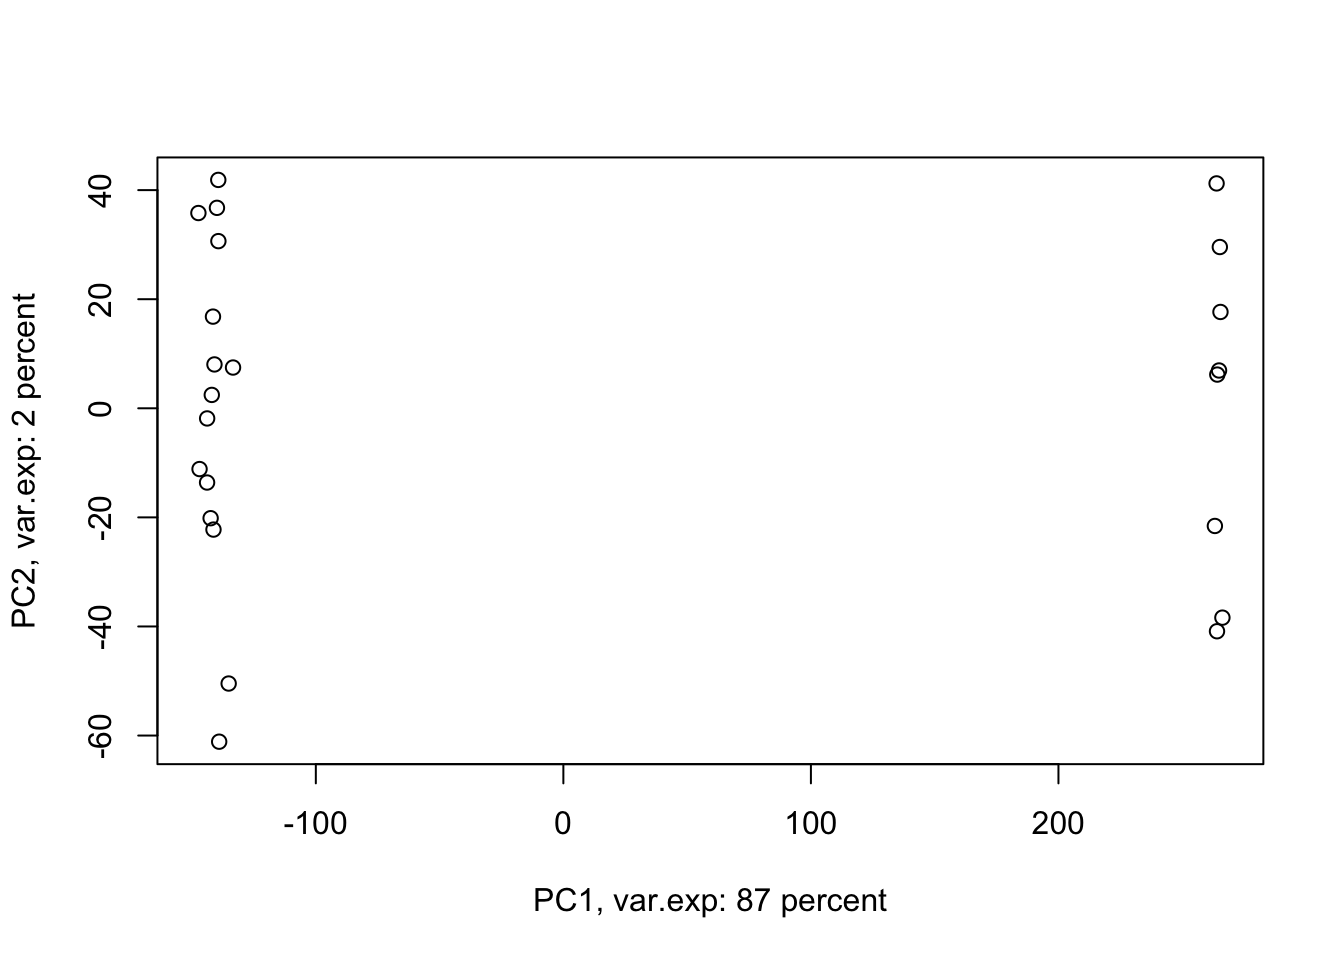
\includegraphics{PCA_files/figure-latex/pcaexample1-1} 

}

\caption{PCA of the data using first two components}\label{fig:pcaexample1}
\end{figure}

Amazing. This is our PCA results. Here in Figure '\ref{fig:pcaexample1}, the x axis is component 1 and the y axis is component 2 of the PCA. We can see that the first compoent alone shows us 87 percent of the total variation in our dataset. This is amazing! we have had 45101 variables with a total of \ensuremath{3.0349908\times 10^{4}} variation. Now we can see 87 percent of the variation (\ensuremath{2.6281803\times 10^{4}}) in only one variable! And look, the second component only explains 2 percent of the total variation so it's not even that important compared to the fist one. But hold on, we first need to see what this new variable actually shows us? Here the statistics does not help much, we as researcher should make sense of this component. By adding shapes, colors etc to the figure, we can start making sense this.

Let's add our group information first:

\begin{Shaded}
\begin{Highlighting}[]
\CommentTok{# set number of figures}
\KeywordTok{par}\NormalTok{(}\DataTypeTok{mfrow=}\KeywordTok{c}\NormalTok{(}\DecValTok{1}\NormalTok{,}\DecValTok{1}\NormalTok{))}

\CommentTok{# calculate variation explained}
\NormalTok{x.var <-}\StringTok{ }\NormalTok{pcaResults}\OperatorTok{$}\NormalTok{sdev }\OperatorTok{^}\StringTok{ }\DecValTok{2}
\NormalTok{x.pvar <-}\StringTok{ }\NormalTok{x.var}\OperatorTok{/}\KeywordTok{sum}\NormalTok{(x.var)}
\NormalTok{x.pvar<-x.pvar}\OperatorTok{*}\DecValTok{100}
\CommentTok{# plot the first two components}
\KeywordTok{plot}\NormalTok{(pcaResults}\OperatorTok{$}\NormalTok{x[,}\DecValTok{1}\OperatorTok{:}\DecValTok{2}\NormalTok{],}\DataTypeTok{xlab=}\KeywordTok{paste}\NormalTok{(}\StringTok{"PC1, var.exp:"}\NormalTok{,}\KeywordTok{round}\NormalTok{(x.pvar[}\DecValTok{1}\NormalTok{]),}\StringTok{"percent"}\NormalTok{),}
     \DataTypeTok{ylab=}\KeywordTok{paste}\NormalTok{(}\StringTok{"PC2, var.exp:"}\NormalTok{,}\KeywordTok{round}\NormalTok{(x.pvar[}\DecValTok{2}\NormalTok{]),}\StringTok{"percent"}\NormalTok{),}\DataTypeTok{col=}\KeywordTok{factor}\NormalTok{(metadata}\OperatorTok{$}\NormalTok{Covariate))}
\CommentTok{# add legend}
\KeywordTok{legend}\NormalTok{(}\StringTok{"top"}\NormalTok{, }\DataTypeTok{legend=}\KeywordTok{c}\NormalTok{(}\KeywordTok{unique}\NormalTok{(}\KeywordTok{levels}\NormalTok{(}\KeywordTok{factor}\NormalTok{(metadata}\OperatorTok{$}\NormalTok{Covariate)))),}
       \DataTypeTok{col=}\KeywordTok{unique}\NormalTok{(}\KeywordTok{as.numeric}\NormalTok{(}\KeywordTok{factor}\NormalTok{(metadata}\OperatorTok{$}\NormalTok{Covariate))), }\DataTypeTok{cex=}\FloatTok{0.8}\NormalTok{, }\DataTypeTok{pch =} \DecValTok{1}\NormalTok{)}
\end{Highlighting}
\end{Shaded}

\begin{figure}

{\centering 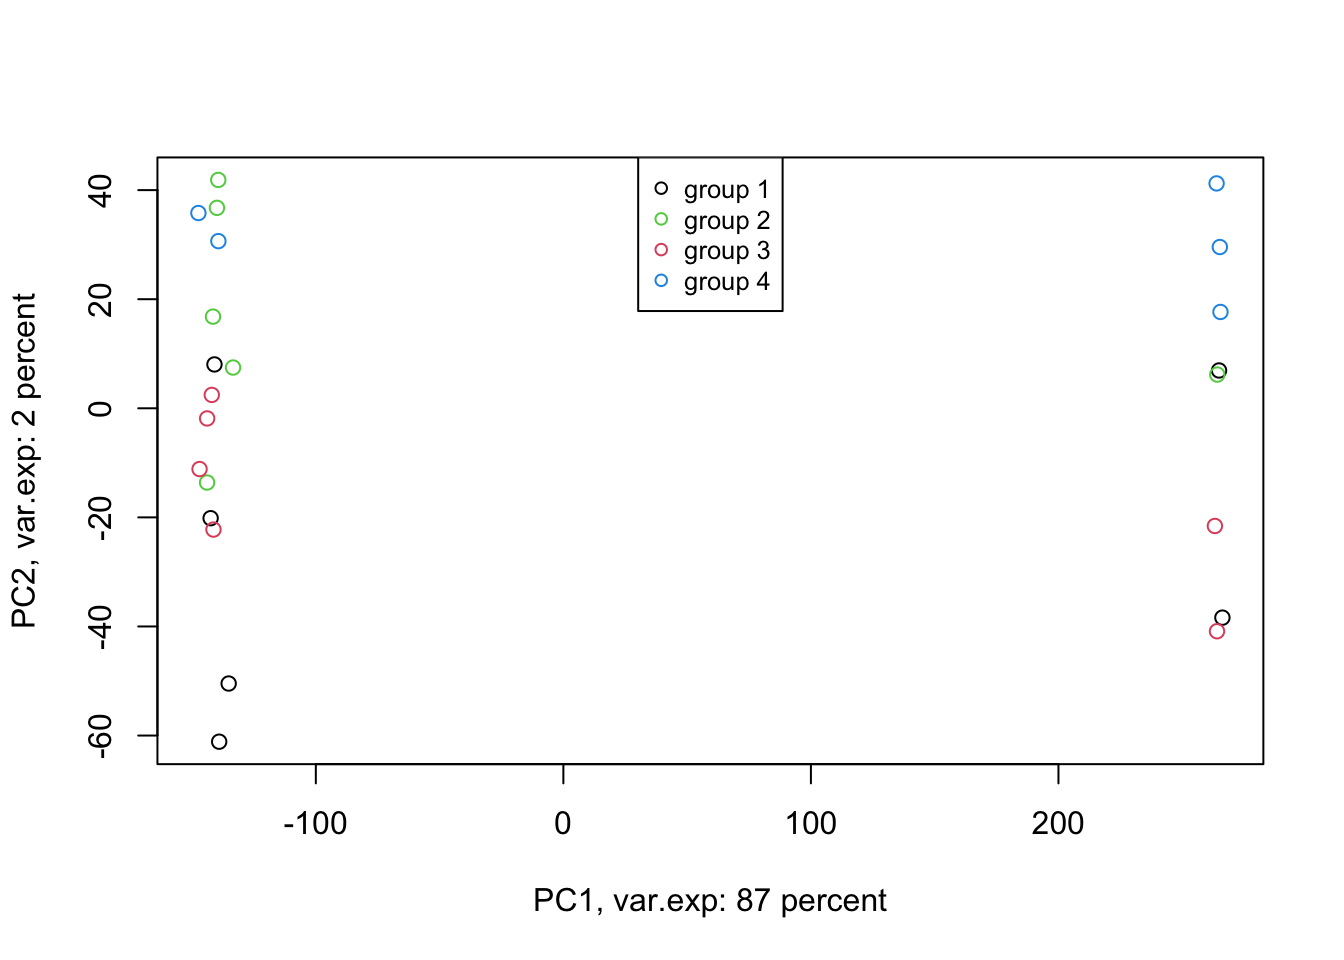
\includegraphics{PCA_files/figure-latex/pcaexample2-1} 

}

\caption{PCA of the data using first two components}\label{fig:pcaexample2}
\end{figure}

Well, OK. Perhaps not something that we actually expected. The largest variation in our data is not coming from difference between our biological groups (e.g.~cancer sub-types). Our group of interest is only visible in the component 2. Remember, we \protect\hyperlink{pcamot}{discussed that PCA is great for finding patterns}, the ones that we don't expect, in an unbiased manner! There is something else in our data that we ignore! That is:

\begin{Shaded}
\begin{Highlighting}[]
\CommentTok{# set number of figures}
\KeywordTok{par}\NormalTok{(}\DataTypeTok{mfrow=}\KeywordTok{c}\NormalTok{(}\DecValTok{1}\NormalTok{,}\DecValTok{1}\NormalTok{))}

\CommentTok{# calculate variation explained}
\NormalTok{x.var <-}\StringTok{ }\NormalTok{pcaResults}\OperatorTok{$}\NormalTok{sdev }\OperatorTok{^}\StringTok{ }\DecValTok{2}
\NormalTok{x.pvar <-}\StringTok{ }\NormalTok{x.var}\OperatorTok{/}\KeywordTok{sum}\NormalTok{(x.var)}
\NormalTok{x.pvar<-x.pvar}\OperatorTok{*}\DecValTok{100}
\CommentTok{# plot the first two components}
\KeywordTok{plot}\NormalTok{(pcaResults}\OperatorTok{$}\NormalTok{x[,}\DecValTok{1}\OperatorTok{:}\DecValTok{2}\NormalTok{],}\DataTypeTok{xlab=}\KeywordTok{paste}\NormalTok{(}\StringTok{"PC1, var.exp:"}\NormalTok{,}\KeywordTok{round}\NormalTok{(x.pvar[}\DecValTok{1}\NormalTok{]),}\StringTok{"percent"}\NormalTok{),}
     \DataTypeTok{ylab=}\KeywordTok{paste}\NormalTok{(}\StringTok{"PC2, var.exp:"}\NormalTok{,}\KeywordTok{round}\NormalTok{(x.pvar[}\DecValTok{2}\NormalTok{]),}\StringTok{"percent"}\NormalTok{),}\DataTypeTok{col=}\KeywordTok{factor}\NormalTok{(metadata}\OperatorTok{$}\NormalTok{Covariate),}\DataTypeTok{pch=}\KeywordTok{as.numeric}\NormalTok{(}\KeywordTok{factor}\NormalTok{(metadata}\OperatorTok{$}\NormalTok{Batch)))}
\CommentTok{# add legend}
\KeywordTok{legend}\NormalTok{(}\StringTok{"center"}\NormalTok{, }\DataTypeTok{legend=}\KeywordTok{paste}\NormalTok{(}\StringTok{"Batch"}\NormalTok{,}\KeywordTok{c}\NormalTok{(}\KeywordTok{unique}\NormalTok{(}\KeywordTok{levels}\NormalTok{(}\KeywordTok{factor}\NormalTok{(metadata}\OperatorTok{$}\NormalTok{Batch))))),}
       \DataTypeTok{pch=}\KeywordTok{unique}\NormalTok{(}\KeywordTok{as.numeric}\NormalTok{(}\KeywordTok{factor}\NormalTok{(metadata}\OperatorTok{$}\NormalTok{Batch))), }\DataTypeTok{cex=}\FloatTok{0.8}\NormalTok{)}
\CommentTok{# add legend}
\KeywordTok{legend}\NormalTok{(}\StringTok{"top"}\NormalTok{, }\DataTypeTok{legend=}\KeywordTok{c}\NormalTok{(}\KeywordTok{unique}\NormalTok{(}\KeywordTok{levels}\NormalTok{(}\KeywordTok{factor}\NormalTok{(metadata}\OperatorTok{$}\NormalTok{Covariate)))),}
       \DataTypeTok{col=}\KeywordTok{unique}\NormalTok{(}\KeywordTok{as.numeric}\NormalTok{(}\KeywordTok{factor}\NormalTok{(metadata}\OperatorTok{$}\NormalTok{Covariate))), }\DataTypeTok{cex=}\FloatTok{0.8}\NormalTok{, }\DataTypeTok{pch =} \DecValTok{1}\NormalTok{)}
\end{Highlighting}
\end{Shaded}

\begin{figure}

{\centering 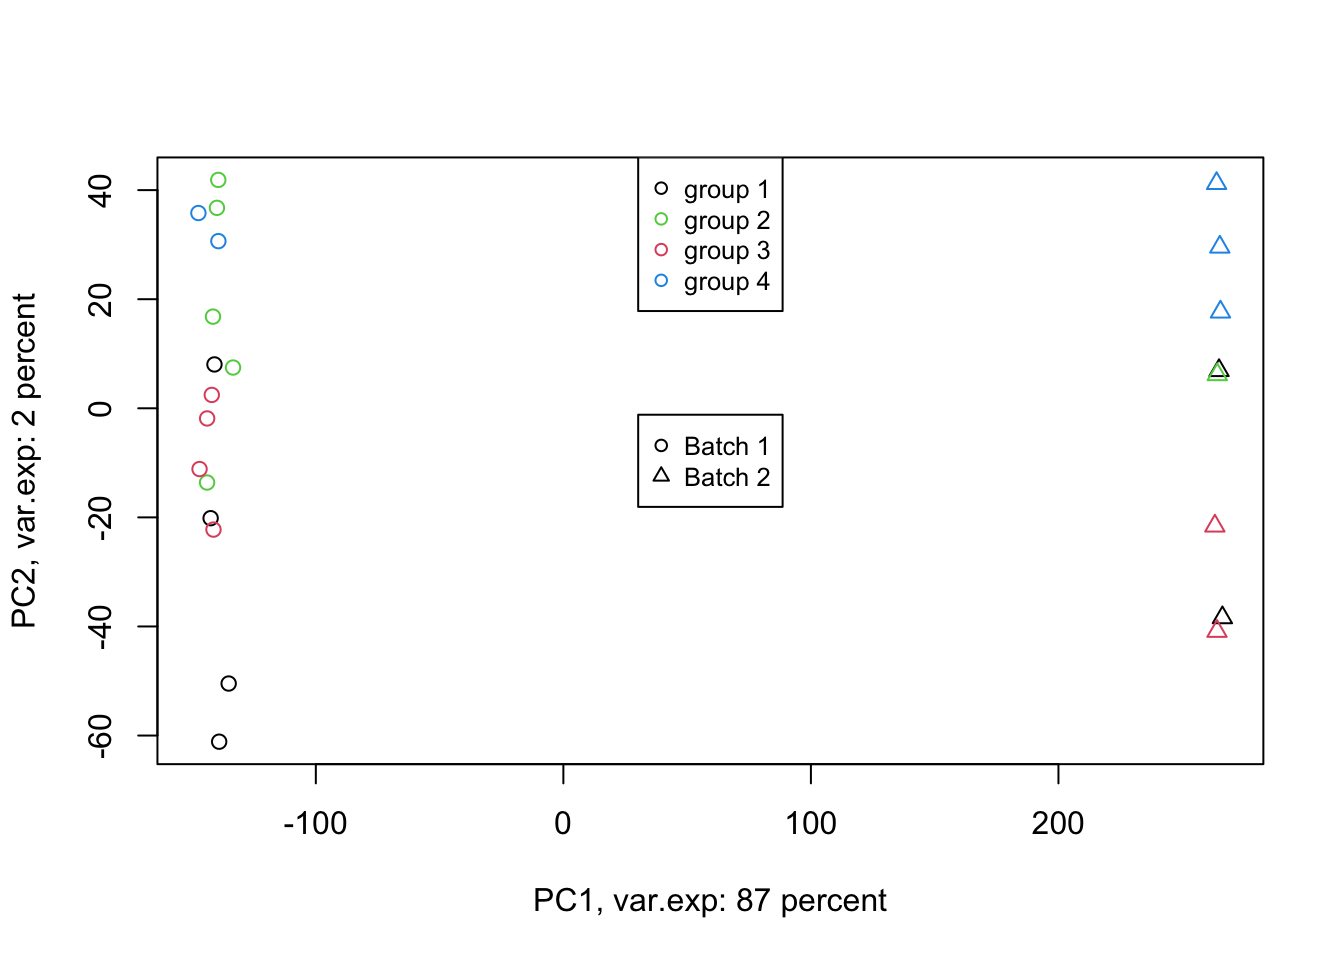
\includegraphics{PCA_files/figure-latex/pcaexample3-1} 

}

\caption{PCA of the data using first two components (v2)}\label{fig:pcaexample3}
\end{figure}

Exactly. We have such a large batch effect between our samples. That is our largest variation. What should we do. Well, we can ignore it go to the next components. Let's go up to ten components:

\begin{Shaded}
\begin{Highlighting}[]
\CommentTok{# set number of figures}
\KeywordTok{par}\NormalTok{(}\DataTypeTok{mfrow=}\KeywordTok{c}\NormalTok{(}\DecValTok{1}\NormalTok{,}\DecValTok{1}\NormalTok{))}

\CommentTok{# calculate variation explained}
\NormalTok{x.var <-}\StringTok{ }\NormalTok{pcaResults}\OperatorTok{$}\NormalTok{sdev }\OperatorTok{^}\StringTok{ }\DecValTok{2}
\NormalTok{x.pvar <-}\StringTok{ }\NormalTok{x.var}\OperatorTok{/}\KeywordTok{sum}\NormalTok{(x.var)}
\NormalTok{x.pvar<-x.pvar}\OperatorTok{*}\DecValTok{100}
\CommentTok{# plot the first two components}
\KeywordTok{pairs}\NormalTok{(pcaResults}\OperatorTok{$}\NormalTok{x[,}\KeywordTok{c}\NormalTok{(}\DecValTok{2}\OperatorTok{:}\DecValTok{10}\NormalTok{)],}
      \DataTypeTok{col=}\KeywordTok{factor}\NormalTok{(metadata}\OperatorTok{$}\NormalTok{Covariate),}\DataTypeTok{pch=}\KeywordTok{as.numeric}\NormalTok{(}\KeywordTok{factor}\NormalTok{(metadata}\OperatorTok{$}\NormalTok{Batch)))}
\end{Highlighting}
\end{Shaded}

\begin{figure}

{\centering 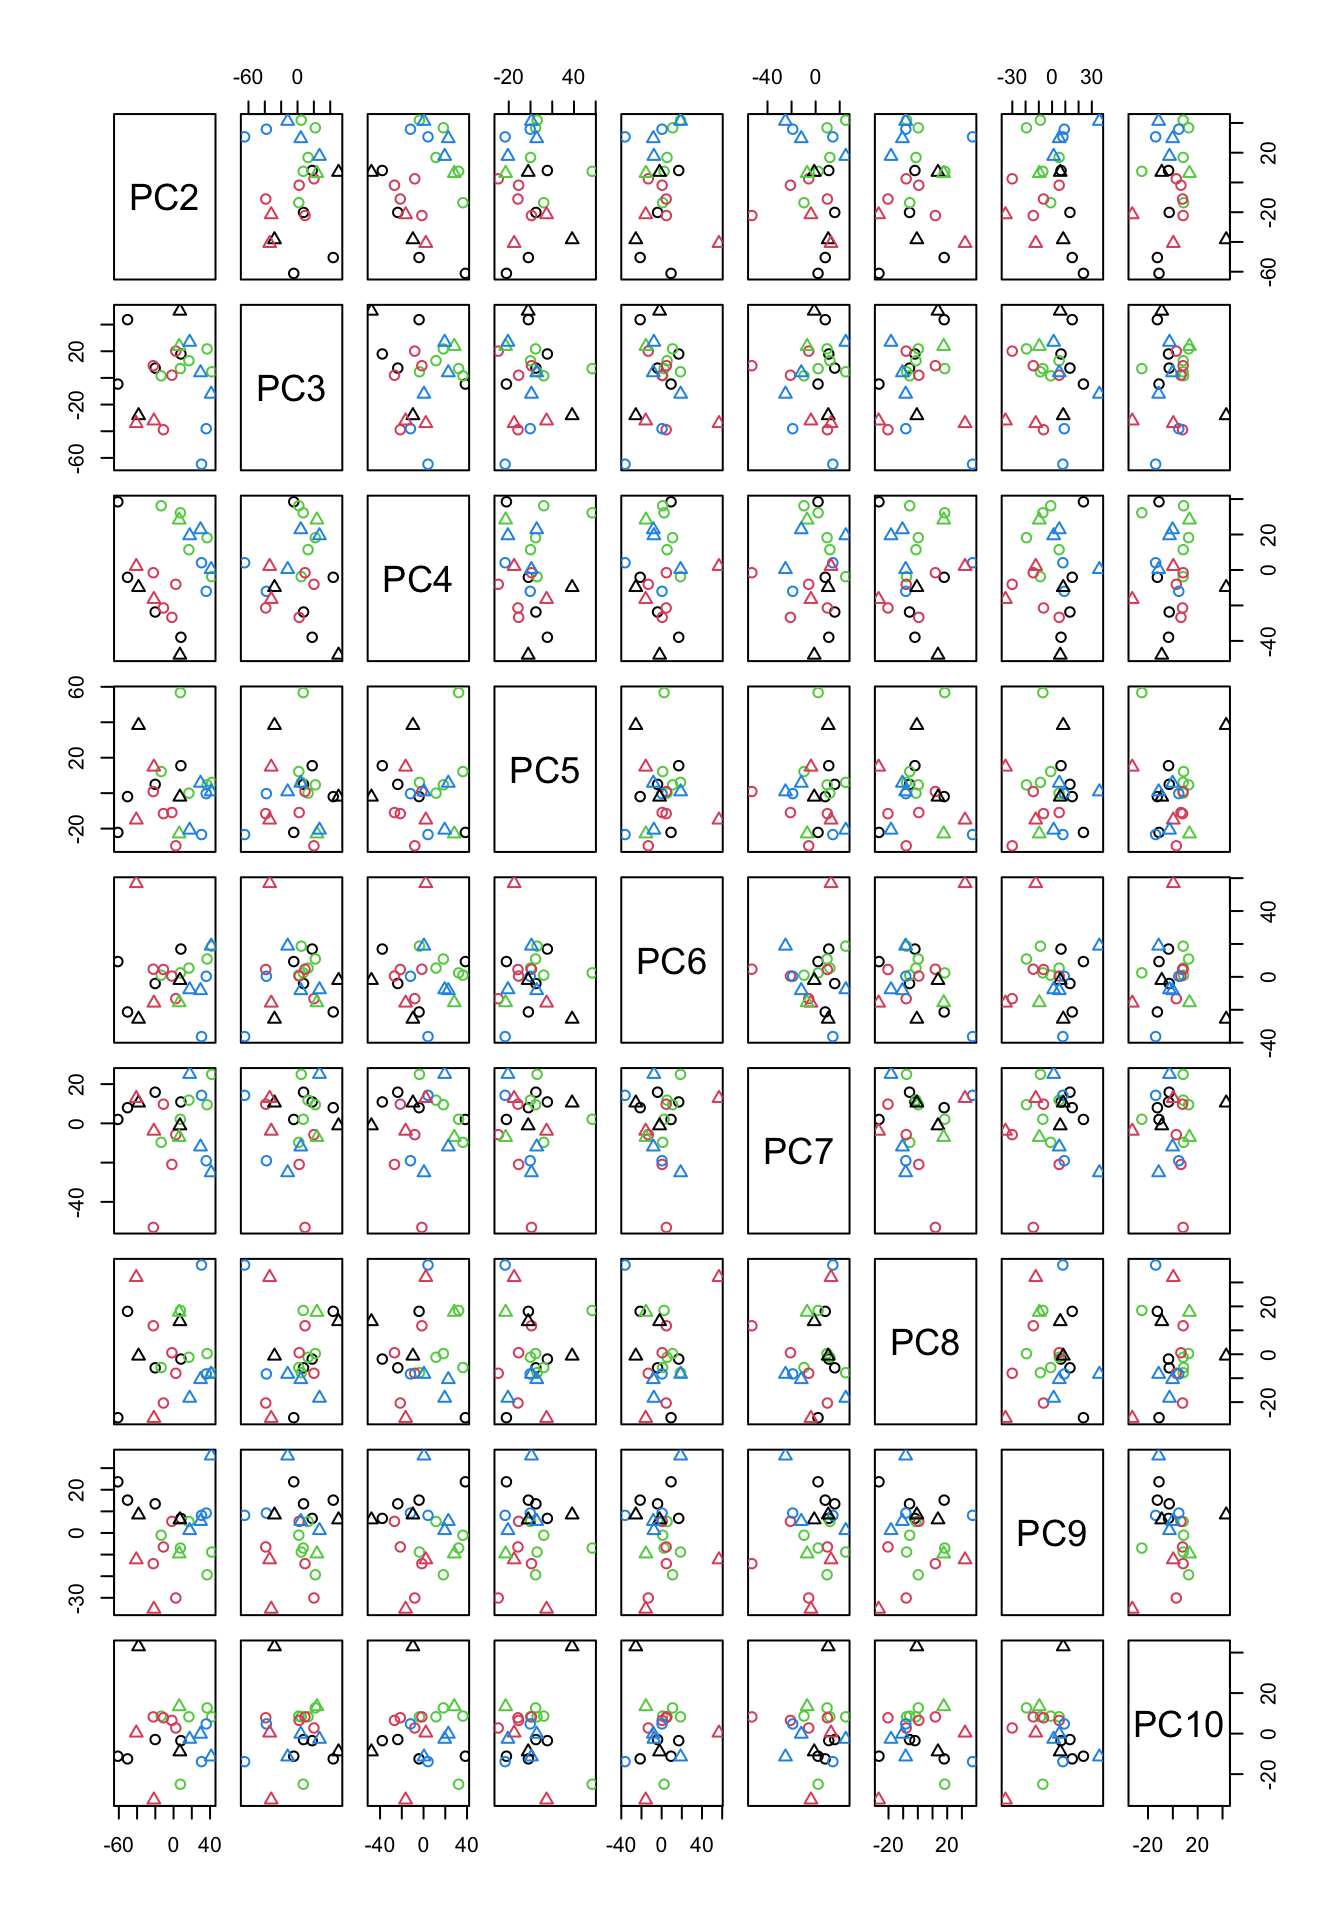
\includegraphics{PCA_files/figure-latex/pcaexample4-1} 

}

\caption{PCA of the data using up to ten components}\label{fig:pcaexample4}
\end{figure}

In Figure \ref{fig:pcaexample4}, we have plotted all possible pairs of components from 2 to 10. This might look scary a bit but If we take a plot in Figure \ref{fig:pcaexample4} which has data points in it, we can figure out what is the x axis but just going up and down and look what ``PC'' is on that column. The same for the y axis. We can just go left and right and figure out which PC is in that row. The combination of PC2 and PC9 looks interesting as they show some group differences.

Let's plot them:

\begin{Shaded}
\begin{Highlighting}[]
\CommentTok{# set number of figures}
\KeywordTok{par}\NormalTok{(}\DataTypeTok{mfrow=}\KeywordTok{c}\NormalTok{(}\DecValTok{1}\NormalTok{,}\DecValTok{1}\NormalTok{))}

\CommentTok{# calculate variation explained}
\NormalTok{x.var <-}\StringTok{ }\NormalTok{pcaResults}\OperatorTok{$}\NormalTok{sdev }\OperatorTok{^}\StringTok{ }\DecValTok{2}
\NormalTok{x.pvar <-}\StringTok{ }\NormalTok{x.var}\OperatorTok{/}\KeywordTok{sum}\NormalTok{(x.var)}
\NormalTok{x.pvar<-x.pvar}\OperatorTok{*}\DecValTok{100}
\CommentTok{# plot the first 2 and 9 components}
\KeywordTok{plot}\NormalTok{(pcaResults}\OperatorTok{$}\NormalTok{x[,}\KeywordTok{c}\NormalTok{(}\DecValTok{2}\NormalTok{,}\DecValTok{9}\NormalTok{)],}\DataTypeTok{xlab=}\KeywordTok{paste}\NormalTok{(}\StringTok{"PC2, var.exp:"}\NormalTok{,}\KeywordTok{round}\NormalTok{(x.pvar[}\DecValTok{2}\NormalTok{]),}\StringTok{"percent"}\NormalTok{),}
     \DataTypeTok{ylab=}\KeywordTok{paste}\NormalTok{(}\StringTok{"PC9, var.exp:"}\NormalTok{,}\KeywordTok{round}\NormalTok{(x.pvar[}\DecValTok{3}\NormalTok{]),}\StringTok{"percent"}\NormalTok{),}\DataTypeTok{col=}\KeywordTok{factor}\NormalTok{(metadata}\OperatorTok{$}\NormalTok{Covariate),}
     \DataTypeTok{pch=}\KeywordTok{as.numeric}\NormalTok{(}\KeywordTok{factor}\NormalTok{(metadata}\OperatorTok{$}\NormalTok{Batch)))}
\CommentTok{# add legend}
\KeywordTok{legend}\NormalTok{(}\StringTok{"top"}\NormalTok{, }\DataTypeTok{legend=}\KeywordTok{c}\NormalTok{(}\KeywordTok{unique}\NormalTok{(}\KeywordTok{levels}\NormalTok{(}\KeywordTok{factor}\NormalTok{(metadata}\OperatorTok{$}\NormalTok{Covariate)))),}
       \DataTypeTok{col=}\KeywordTok{unique}\NormalTok{(}\KeywordTok{as.numeric}\NormalTok{(}\KeywordTok{factor}\NormalTok{(metadata}\OperatorTok{$}\NormalTok{Covariate))), }\DataTypeTok{cex=}\FloatTok{0.8}\NormalTok{, }\DataTypeTok{pch =} \DecValTok{1}\NormalTok{)}

\CommentTok{# add legend}
\KeywordTok{legend}\NormalTok{(}\StringTok{"topleft"}\NormalTok{, }\DataTypeTok{legend=}\KeywordTok{paste}\NormalTok{(}\StringTok{"Batch"}\NormalTok{,}\KeywordTok{c}\NormalTok{(}\KeywordTok{unique}\NormalTok{(}\KeywordTok{levels}\NormalTok{(}\KeywordTok{factor}\NormalTok{(metadata}\OperatorTok{$}\NormalTok{Batch))))),}
       \DataTypeTok{pch=}\KeywordTok{unique}\NormalTok{(}\KeywordTok{as.numeric}\NormalTok{(}\KeywordTok{factor}\NormalTok{(metadata}\OperatorTok{$}\NormalTok{Batch))), }\DataTypeTok{cex=}\FloatTok{0.8}\NormalTok{)}
\end{Highlighting}
\end{Shaded}

\begin{figure}

{\centering 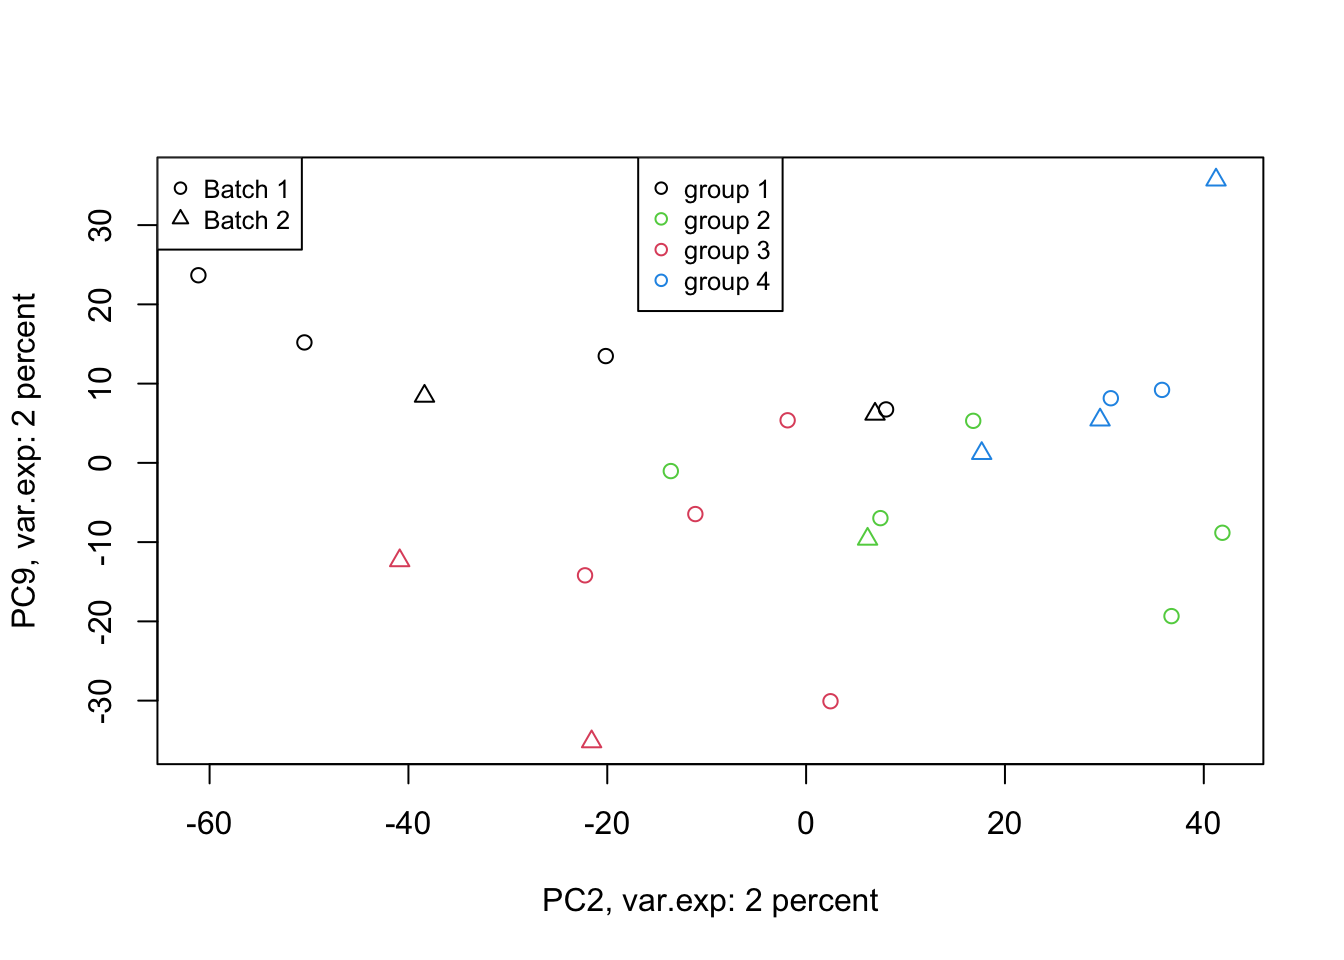
\includegraphics{PCA_files/figure-latex/pcaexample5-1} 

}

\caption{PCA of the data 2 and 9 components}\label{fig:pcaexample5}
\end{figure}

That is not that bad! We can see differences between groups of interest and not batch effect. So we can conclude that there is certainly some differences between the groups but it's much lower than our experimental factors (such as batch or others that we don't know!). So our experiment has been successful. Please also note that, if you see the variation of interest in the first components, it's generally a good sign (unless there is confounding somewhere) as PCA found what you wanted without knowing it, meaning that the signal has been very strong compared to noise! Now we want to move one step back and ask given the differences we see in these new variables, what can we say about the original variables (e.g.~genes). Are there some genes specific responsible for these differences that we see? Or What are the genes that are influence by group (cancer sub-types) or even batches? This is the topic the next secion.

\hypertarget{pcavarselect}{%
\section{Variable selection}\label{pcavarselect}}

In many experiments, we are not only interested in seeing whether the experiment has been successful, but we are also interested in know whether any of the measurements (variables) have been affected let's say by some kind of perturbation? Variable selection is the key to answer this question. In short, we are going to single out the variables that might be of interest for further investigation. Some examples can be performing t-test or regression and deciding which variables are ``statistically significant''. PCA also gives us a tool to do so. However, it does that without a need to do statistical testing.

If we recall, in Table \ref{tab:tabpca2}, we had another element (returned by PCA) that is called \emph{rotation}. What are these? We have been repeatedly saying that PCA creates new variables that are \textbf{combinations} of the original variable. We can think about a combination like \emph{New variable (let's say component 1) = original variable 1 + original variable 2 + original variable 3}. However, PCA adds a little more! It adds weights to the original variables and then combine them. So the new variable is the weighted combination of the original ones. These weights \textbf{in each component} are indications of importance or influence of a particular variable on the data pattern we see in a component. These weight can be positive or negative, but for now, the larger the absolute value, the more interesting the variable is for us. At the end please note that these weights \emph{rotations} are also called loadings in many contexts.

Having this said let's have a look at the \emph{rotation}:

\begin{Shaded}
\begin{Highlighting}[]
\CommentTok{# make a table}
\NormalTok{knitr}\OperatorTok{::}\KeywordTok{kable}\NormalTok{(pcaResults}\OperatorTok{$}\NormalTok{rotation[}\DecValTok{1}\OperatorTok{:}\DecValTok{5}\NormalTok{,}\DecValTok{1}\OperatorTok{:}\DecValTok{5}\NormalTok{],}
             \DataTypeTok{caption =} \StringTok{"PCA output rotation (only top 5 are shown)"}\NormalTok{)}
\end{Highlighting}
\end{Shaded}

\begin{table}

\caption{\label{tab:tabpca3}PCA output rotation (only top 5 are shown)}
\centering
\begin{tabular}[t]{r|r|r|r|r}
\hline
PC1 & PC2 & PC3 & PC4 & PC5\\
\hline
0.0046596 & -0.0015491 & -0.0050678 & -0.0013241 & 0.0030454\\
\hline
0.0044884 & -0.0020155 & -0.0023613 & -0.0061551 & -0.0025862\\
\hline
0.0046884 & -0.0038413 & 0.0016769 & 0.0037431 & 0.0104244\\
\hline
0.0049866 & -0.0010551 & -0.0030093 & 0.0018562 & 0.0009776\\
\hline
0.0047319 & -0.0029789 & 0.0029067 & -0.0035312 & 0.0034596\\
\hline
\end{tabular}
\end{table}

In Table \ref{tab:tabpca3}, we only show five variables (weights) for five components but in fact there are 23 components (PCs) for each we have 45101 weights.
The way the we do variable selection is, for the component of interest we sort the absolute values of these weights in descending order, and the select top x highest variables (let's say top 5 if we only want 5 variables). For this experiment, we have already select the component 2 and 9 to be important for us. Now let's select top 5 variables for each component.

\begin{Shaded}
\begin{Highlighting}[]
\CommentTok{# set number of figures}
\KeywordTok{par}\NormalTok{(}\DataTypeTok{mfrow=}\KeywordTok{c}\NormalTok{(}\DecValTok{2}\NormalTok{,}\DecValTok{1}\NormalTok{),}\DataTypeTok{las=}\DecValTok{2}\NormalTok{)}


\NormalTok{PC2_rotations<-pcaResults}\OperatorTok{$}\NormalTok{rotation[}\KeywordTok{order}\NormalTok{(}\KeywordTok{abs}\NormalTok{(pcaResults}\OperatorTok{$}\NormalTok{rotation[,}\DecValTok{2}\NormalTok{]),}\DataTypeTok{decreasing =}\NormalTok{ T)[}\DecValTok{1}\OperatorTok{:}\DecValTok{5}\NormalTok{],}\DecValTok{2}\NormalTok{]}

\KeywordTok{names}\NormalTok{(PC2_rotations)<-}\KeywordTok{as.character}\NormalTok{(}\KeywordTok{order}\NormalTok{(}\KeywordTok{abs}\NormalTok{(pcaResults}\OperatorTok{$}\NormalTok{rotation[,}\DecValTok{2}\NormalTok{]),}\DataTypeTok{decreasing =}\NormalTok{ T)[}\DecValTok{1}\OperatorTok{:}\DecValTok{5}\NormalTok{])}
\NormalTok{PC2_rotations<-}\KeywordTok{rev}\NormalTok{(}\KeywordTok{abs}\NormalTok{(PC2_rotations))                                 }
\KeywordTok{barplot}\NormalTok{(PC2_rotations,}\DataTypeTok{horiz=}\OtherTok{TRUE}\NormalTok{,}\DataTypeTok{main =} \StringTok{"Component 2"}\NormalTok{)}
\CommentTok{# add legend}
\CommentTok{# set number of figures}



\NormalTok{PC9_rotations<-pcaResults}\OperatorTok{$}\NormalTok{rotation[}\KeywordTok{order}\NormalTok{(}\KeywordTok{abs}\NormalTok{(pcaResults}\OperatorTok{$}\NormalTok{rotation[,}\DecValTok{9}\NormalTok{]),}\DataTypeTok{decreasing =}\NormalTok{ T)[}\DecValTok{1}\OperatorTok{:}\DecValTok{5}\NormalTok{],}\DecValTok{9}\NormalTok{]}

\KeywordTok{names}\NormalTok{(PC9_rotations)<-}\KeywordTok{as.character}\NormalTok{(}\KeywordTok{order}\NormalTok{(}\KeywordTok{abs}\NormalTok{(pcaResults}\OperatorTok{$}\NormalTok{rotation[,}\DecValTok{9}\NormalTok{]),}\DataTypeTok{decreasing =}\NormalTok{ T)[}\DecValTok{1}\OperatorTok{:}\DecValTok{5}\NormalTok{])}
\NormalTok{PC9_rotations<-}\KeywordTok{rev}\NormalTok{(}\KeywordTok{abs}\NormalTok{(PC9_rotations))   }
\KeywordTok{barplot}\NormalTok{(PC9_rotations,}\DataTypeTok{horiz=}\OtherTok{TRUE}\NormalTok{,}\DataTypeTok{main =} \StringTok{"Component 9"}\NormalTok{)}
\end{Highlighting}
\end{Shaded}

\begin{figure}

{\centering 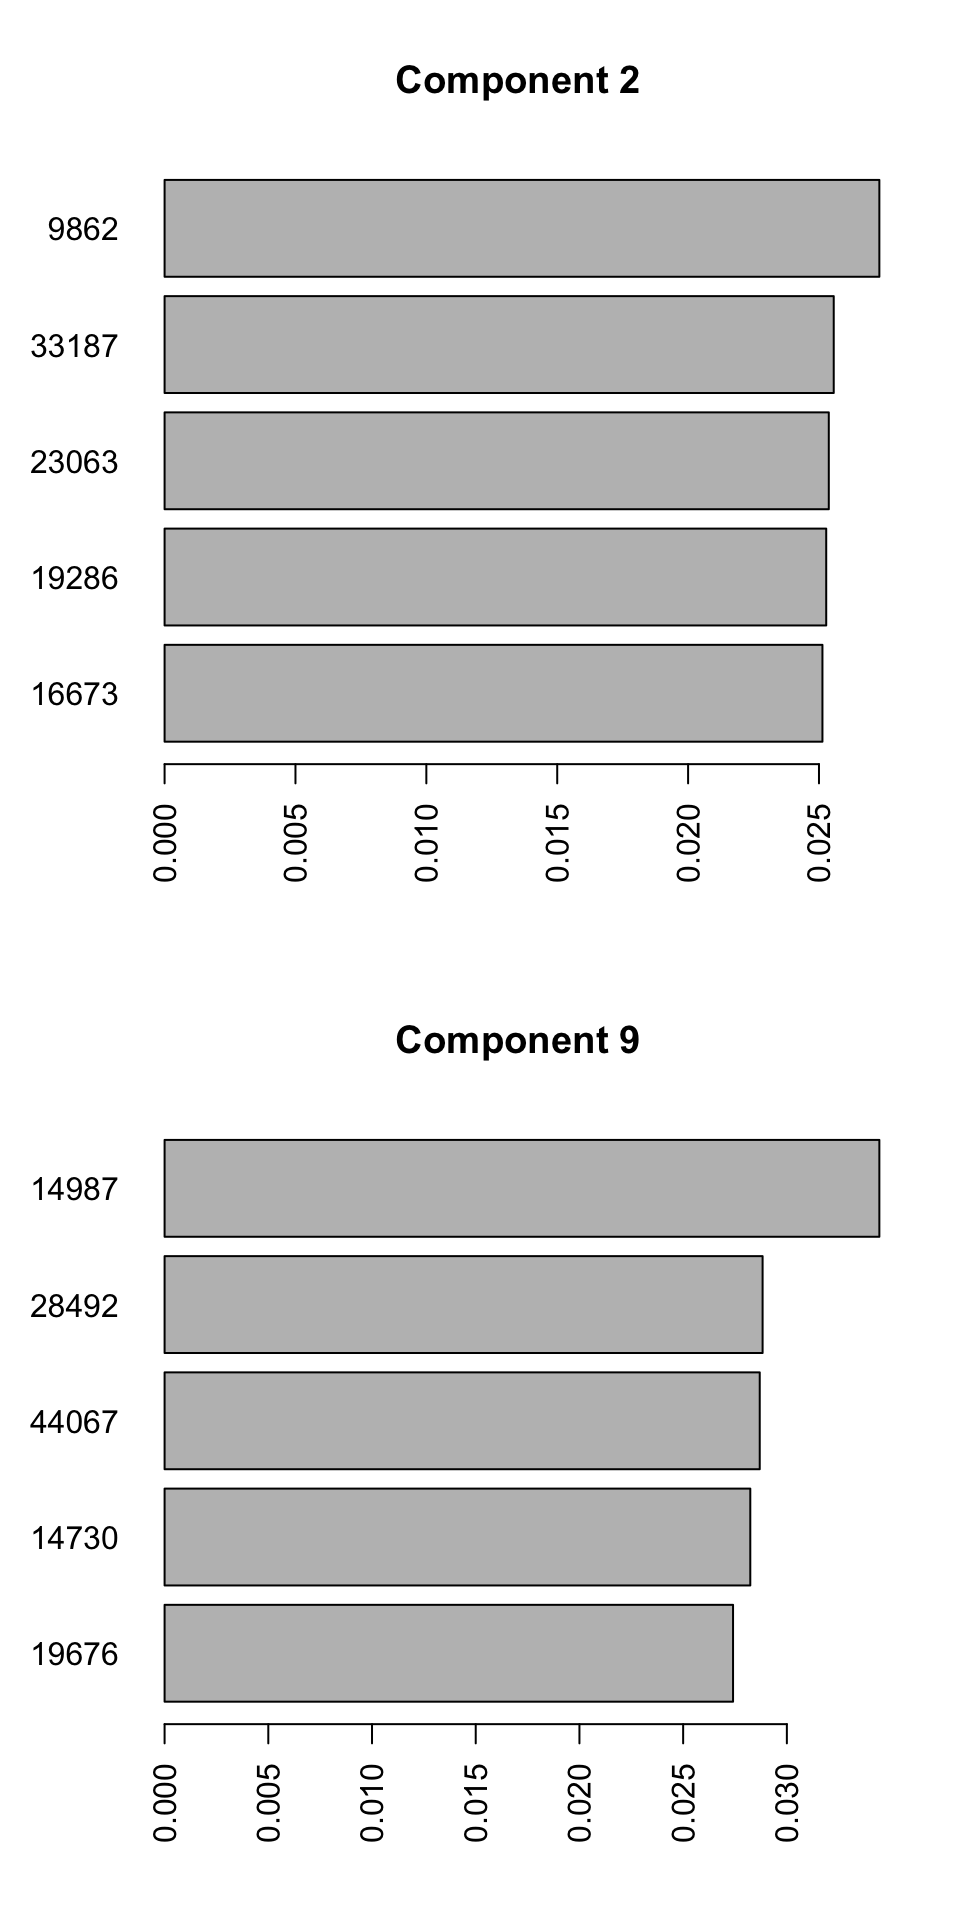
\includegraphics{PCA_files/figure-latex/pcaexample6-1} 

}

\caption{Selecting top five variables for components 2 and 9}\label{fig:pcaexample6}
\end{figure}

We can see the name of the variable on the y axis and its contribution on the x axis. So we have 10 unique variables (the variables can sometime overlap between different components). We will have to interpret these variables together with \protect\hyperlink{pcaexample5}{components}. Because we see differences between groups 2, 3 and 4 in the second components, variables selected for this component influence the differences between the mentioned groups. The variables selected for the component 9, will mostly influence the differences between group 1 and the rest. It will take some time to get used to this kind of interpretation but after a while it will become very convenient to do variable selection using PCA. This way, we can avoid doing statistical testing, and thus avoid multiple testing problem. In addition, we can easily remove variables to avoid for example overfitting of statistical models and many other advantages.
We can have a look at the variables we selected in isolation:

\begin{Shaded}
\begin{Highlighting}[]
\CommentTok{# set number of figures}
\KeywordTok{par}\NormalTok{(}\DataTypeTok{mfrow=}\KeywordTok{c}\NormalTok{(}\DecValTok{2}\NormalTok{,}\DecValTok{5}\NormalTok{))}

\ControlFlowTok{for}\NormalTok{(x }\ControlFlowTok{in} \KeywordTok{names}\NormalTok{(}\KeywordTok{sort}\NormalTok{(PC2_rotations,}\DataTypeTok{decreasing =}\NormalTok{ T)))}
\NormalTok{\{}
  \CommentTok{# plot the data}
\NormalTok{  dt<-data[,}\KeywordTok{as.numeric}\NormalTok{(x)]}
\KeywordTok{plot}\NormalTok{(}\DataTypeTok{x=}\NormalTok{dt,}\DataTypeTok{y=}\KeywordTok{rep}\NormalTok{(}\DecValTok{1}\NormalTok{,}\KeywordTok{nrow}\NormalTok{(data)),}\DataTypeTok{axes =}\NormalTok{ F,}\DataTypeTok{ylab =} \StringTok{""}\NormalTok{,}\DataTypeTok{xlab =} \KeywordTok{paste}\NormalTok{(}\StringTok{"PC2,"}\NormalTok{,x,}\DataTypeTok{sep=}\StringTok{""}\NormalTok{),}\DataTypeTok{col=}\KeywordTok{factor}\NormalTok{(metadata}\OperatorTok{$}\NormalTok{Covariate))}
\KeywordTok{axis}\NormalTok{(}\DecValTok{1}\NormalTok{,}\DataTypeTok{cex=}\DecValTok{4}\NormalTok{,}\DataTypeTok{pos =} \KeywordTok{c}\NormalTok{(}\FloatTok{0.9}\NormalTok{,}\FloatTok{0.5}\NormalTok{) )}

\NormalTok{\}}

\ControlFlowTok{for}\NormalTok{(x }\ControlFlowTok{in} \KeywordTok{names}\NormalTok{(}\KeywordTok{sort}\NormalTok{(PC9_rotations,}\DataTypeTok{decreasing =}\NormalTok{ T)))}
\NormalTok{\{}
  \CommentTok{# plot the data}
\NormalTok{  dt<-data[,}\KeywordTok{as.numeric}\NormalTok{(x)]}
\KeywordTok{plot}\NormalTok{(}\DataTypeTok{x=}\NormalTok{dt,}\DataTypeTok{y=}\KeywordTok{rep}\NormalTok{(}\DecValTok{1}\NormalTok{,}\KeywordTok{nrow}\NormalTok{(data)),}\DataTypeTok{axes =}\NormalTok{ F,}\DataTypeTok{ylab =} \StringTok{""}\NormalTok{,}\DataTypeTok{xlab =} \KeywordTok{paste}\NormalTok{(}\StringTok{"PC9,"}\NormalTok{,x,}\DataTypeTok{sep=}\StringTok{""}\NormalTok{),}\DataTypeTok{col=}\KeywordTok{factor}\NormalTok{(metadata}\OperatorTok{$}\NormalTok{Covariate))}
\KeywordTok{axis}\NormalTok{(}\DecValTok{1}\NormalTok{,}\DataTypeTok{cex=}\DecValTok{4}\NormalTok{,}\DataTypeTok{pos =} \KeywordTok{c}\NormalTok{(}\FloatTok{0.9}\NormalTok{,}\FloatTok{0.5}\NormalTok{) )}

\NormalTok{\}}
\end{Highlighting}
\end{Shaded}

\begin{figure}

{\centering 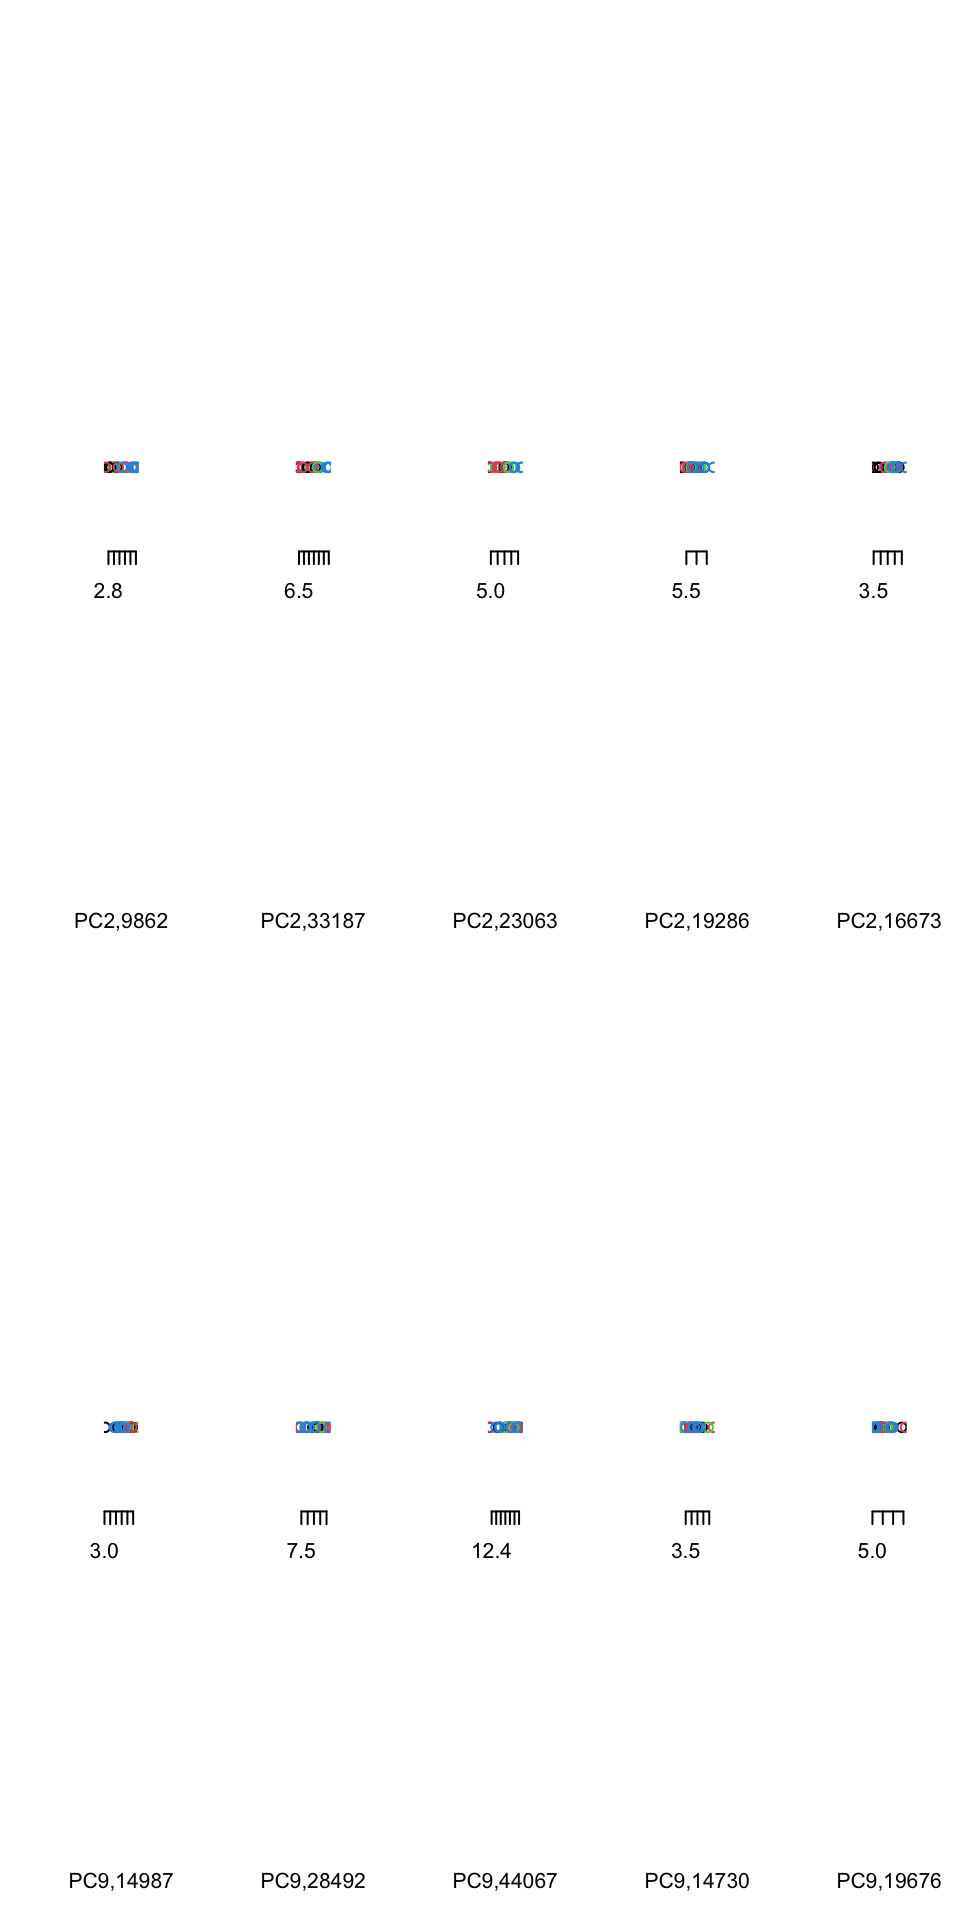
\includegraphics{PCA_files/figure-latex/pcaexample7-1} 

}

\caption{Top 5 variables per component are plotted}\label{fig:pcaexample7}
\end{figure}

We can see that, in case of component 2, most variable show the same trend that the component 2 showed us. However, This is not the case in the component 9 where there is only one or maybe two variables (28492 and 44067) that showed what component 9 showed. There are several reasons for this, including:

\begin{itemize}
\tightlist
\item
  PCA looks where most of the variation is without knowing about the groups. We can see that there is single observation in for example variable 14987 that is very different compared to the rest of the observation.
\item
  PCA components are combinations of \textbf{all} the variables. Simply because we chose to select the top five variables does not mean the rest of the variables are not influencing the pattern
\item
  From the PCA perspective, this variables are top ones. This does not mean that they will answer our research question. That is of course up to us what to conclude!
\item
  The distances between the observations in the PCA components would have been the same as the orginal data IF you did not remove any components. Now that we decided to remove some components, the distances are not the same.
\end{itemize}

By now you should have a good understanding of application PCA for dimentionality reduction and visualization. We could squeeze our dataset with 45101 variables to a few ones still showing the overall data pattern. We could also extract variables with most influence on the data for the purpose of further investigations.

We could stop here and you are good to start using PCA. But there is one more thing to talk about. Let's move to the last section of this chapter.

\hypertarget{pcabtrm}{%
\section{Batch removing (removing variation)}\label{pcabtrm}}

Working with PCA components is nice, their are standarized, they have specific meaning but there are situations that we want to work on the original data. However, maybe we find a variation of interest in a few PCA components and we have to keep that variation and remove the rest. Or it also can be that we found a variation that is not of interest and we want to remove it and keep the rest. The example would the batch effect that we saw \protect\hyperlink{pcaexample1}{before}. Maybe we want to remove batch effect from our data. PCA will give us a very power tool to do so. Let's have another look at the previous batch effect. We also select top two variables affected by the batch effect and plot them

\begin{Shaded}
\begin{Highlighting}[]
\CommentTok{# set number of figures}
\KeywordTok{par}\NormalTok{(}\DataTypeTok{mfrow =} \KeywordTok{c}\NormalTok{(}\DecValTok{1}\NormalTok{, }\DecValTok{2}\NormalTok{))}

\CommentTok{# calculate variation explained}
\NormalTok{x.var <-}\StringTok{ }\NormalTok{pcaResults}\OperatorTok{$}\NormalTok{sdev}\OperatorTok{^}\DecValTok{2}
\NormalTok{x.pvar <-}\StringTok{ }\NormalTok{x.var}\OperatorTok{/}\KeywordTok{sum}\NormalTok{(x.var)}
\NormalTok{x.pvar <-}\StringTok{ }\NormalTok{x.pvar }\OperatorTok{*}\StringTok{ }\DecValTok{100}
\CommentTok{# plot the first two components}
\KeywordTok{plot}\NormalTok{(pcaResults}\OperatorTok{$}\NormalTok{x[, }\DecValTok{1}\OperatorTok{:}\DecValTok{2}\NormalTok{], }\DataTypeTok{xlab =} \KeywordTok{paste}\NormalTok{(}\StringTok{"PC1, var.exp:"}\NormalTok{, }\KeywordTok{round}\NormalTok{(x.pvar[}\DecValTok{1}\NormalTok{]), }\StringTok{"percent"}\NormalTok{), }\DataTypeTok{ylab =} \KeywordTok{paste}\NormalTok{(}\StringTok{"PC2, var.exp:"}\NormalTok{, }\KeywordTok{round}\NormalTok{(x.pvar[}\DecValTok{2}\NormalTok{]), }\StringTok{"percent"}\NormalTok{), }\DataTypeTok{pch =} \KeywordTok{as.numeric}\NormalTok{(}\KeywordTok{factor}\NormalTok{(metadata}\OperatorTok{$}\NormalTok{Batch)))}
\CommentTok{# plot title}
\KeywordTok{title}\NormalTok{(}\StringTok{"PCA batch effect"}\NormalTok{)}

\CommentTok{# add legend}
\KeywordTok{legend}\NormalTok{(}\StringTok{"top"}\NormalTok{, }\DataTypeTok{legend =} \KeywordTok{paste}\NormalTok{(}\StringTok{"Batch"}\NormalTok{, }\KeywordTok{c}\NormalTok{(}\KeywordTok{unique}\NormalTok{(}\KeywordTok{levels}\NormalTok{(}\KeywordTok{factor}\NormalTok{(metadata}\OperatorTok{$}\NormalTok{Batch))))), }\DataTypeTok{pch =} \KeywordTok{unique}\NormalTok{(}\KeywordTok{as.numeric}\NormalTok{(}\KeywordTok{factor}\NormalTok{(metadata}\OperatorTok{$}\NormalTok{Batch))), }\DataTypeTok{cex =} \FloatTok{0.8}\NormalTok{)}

\CommentTok{# }
\NormalTok{PC1_rotations <-}\StringTok{ }\NormalTok{pcaResults}\OperatorTok{$}\NormalTok{rotation[}\KeywordTok{order}\NormalTok{(}\KeywordTok{abs}\NormalTok{(pcaResults}\OperatorTok{$}\NormalTok{rotation[, }\DecValTok{1}\NormalTok{]), }\DataTypeTok{decreasing =}\NormalTok{ T)[}\DecValTok{1}\OperatorTok{:}\DecValTok{2}\NormalTok{], }\DecValTok{1}\NormalTok{]}

\KeywordTok{names}\NormalTok{(PC1_rotations) <-}\StringTok{ }\NormalTok{(}\KeywordTok{order}\NormalTok{(}\KeywordTok{abs}\NormalTok{(pcaResults}\OperatorTok{$}\NormalTok{rotation[, }\DecValTok{1}\NormalTok{]), }\DataTypeTok{decreasing =}\NormalTok{ T)[}\DecValTok{1}\OperatorTok{:}\DecValTok{2}\NormalTok{])}

\KeywordTok{plot}\NormalTok{(data[, (}\KeywordTok{order}\NormalTok{(}\KeywordTok{abs}\NormalTok{(pcaResults}\OperatorTok{$}\NormalTok{rotation[, }\DecValTok{1}\NormalTok{]), }\DataTypeTok{decreasing =}\NormalTok{ T)[}\DecValTok{1}\OperatorTok{:}\DecValTok{2}\NormalTok{])], }\DataTypeTok{xlab =} \KeywordTok{paste}\NormalTok{(}\StringTok{"Variable"}\NormalTok{, }\KeywordTok{names}\NormalTok{(PC1_rotations)[}\DecValTok{1}\NormalTok{]), }\DataTypeTok{ylab =} \KeywordTok{paste}\NormalTok{(}\StringTok{"Variable"}\NormalTok{, }\KeywordTok{names}\NormalTok{(PC1_rotations)[}\DecValTok{2}\NormalTok{]), }\DataTypeTok{pch =} \KeywordTok{as.numeric}\NormalTok{(}\KeywordTok{factor}\NormalTok{(metadata}\OperatorTok{$}\NormalTok{Batch)))}
\KeywordTok{title}\NormalTok{(}\StringTok{"Original variables"}\NormalTok{)}
\end{Highlighting}
\end{Shaded}

\begin{figure}

{\centering 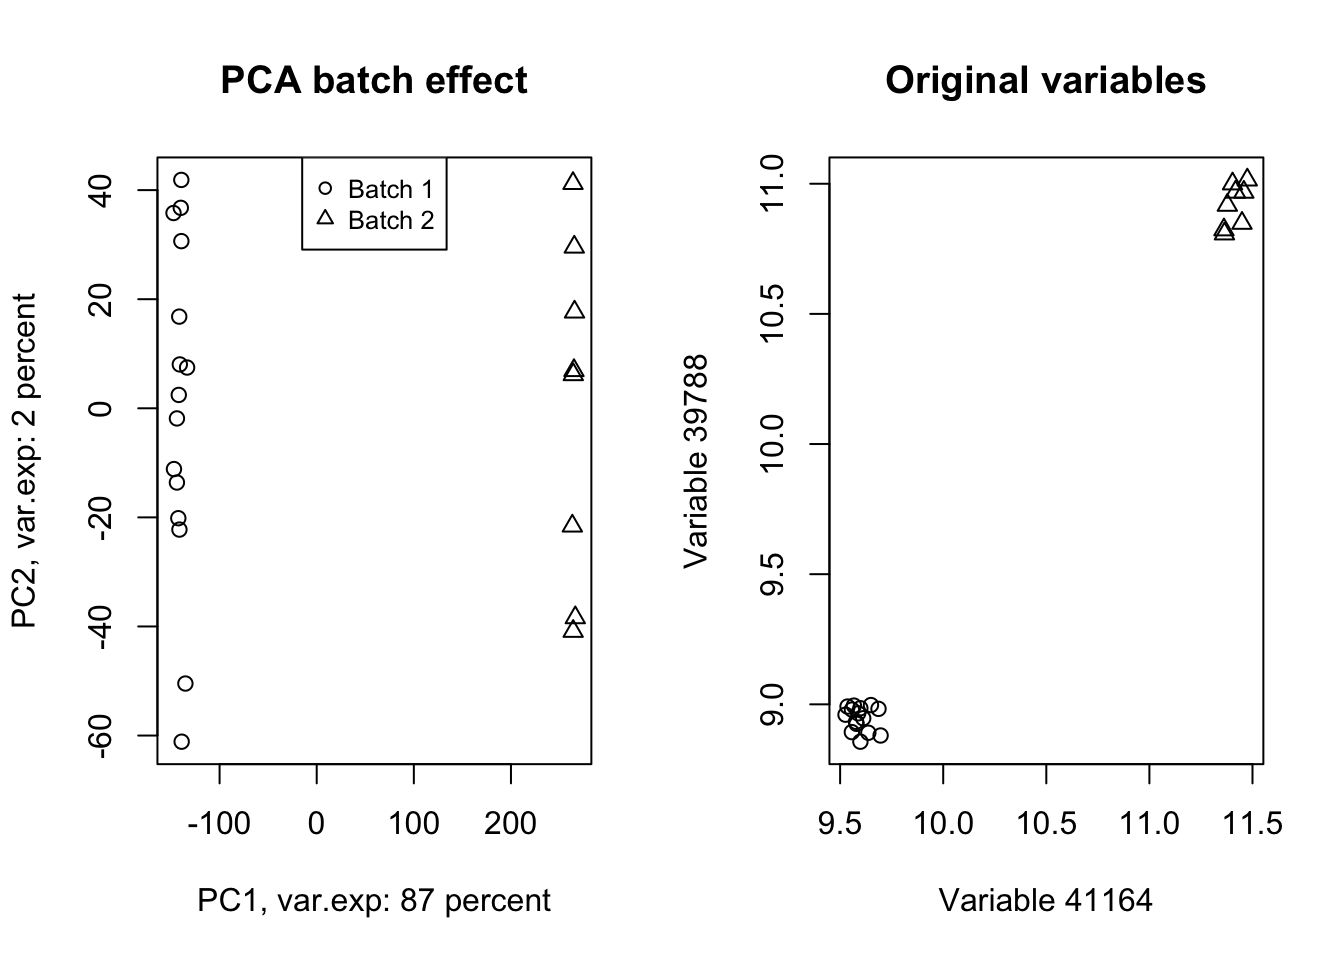
\includegraphics{PCA_files/figure-latex/pcabatch1-1} 

}

\caption{PCA of the data showing the batch effect in our data}\label{fig:pcabatch1}
\end{figure}

Wow! Look at how the variables have been affected by batch effect. Now we do a trick (we will go through this in detail later) and ignore the component one and tell PCA to rebuild our dataset without that component but including all other components.

\begin{Shaded}
\begin{Highlighting}[]
\CommentTok{# set number of figures}
\KeywordTok{par}\NormalTok{(}\DataTypeTok{mfrow=}\KeywordTok{c}\NormalTok{(}\DecValTok{1}\NormalTok{,}\DecValTok{2}\NormalTok{))}

\CommentTok{# Reconstruct the data without the first component}
\NormalTok{new_data<-pcaResults}\OperatorTok{$}\NormalTok{x[,}\OperatorTok{-}\DecValTok{1}\NormalTok{]}\OperatorTok\KeywordTok{t}\NormalTok{(pcaResults}\OperatorTok{$}\NormalTok{rotation[,}\OperatorTok{-}\DecValTok{1}\NormalTok{])}

\CommentTok{# rescale and recenter the data}
\NormalTok{new_data<-}\KeywordTok{scale}\NormalTok{(new_data,}\DataTypeTok{scale =} \DecValTok{1}\OperatorTok{/}\NormalTok{pcaResults}\OperatorTok{$}\NormalTok{scale,}\DataTypeTok{center =} \DecValTok{-1}\OperatorTok{*}\NormalTok{pcaResults}\OperatorTok{$}\NormalTok{center)}

\CommentTok{# do another PCA}
\NormalTok{pcaResults_new<-}\KeywordTok{prcomp}\NormalTok{(new_data,}\DataTypeTok{center =}\NormalTok{ T,}\DataTypeTok{scale. =}\NormalTok{ T)}
\CommentTok{# calculate variation explained}
\NormalTok{x.var <-}\StringTok{ }\NormalTok{pcaResults_new}\OperatorTok{$}\NormalTok{sdev }\OperatorTok{^}\StringTok{ }\DecValTok{2}
\NormalTok{x.pvar <-}\StringTok{ }\NormalTok{x.var}\OperatorTok{/}\KeywordTok{sum}\NormalTok{(x.var)}
\NormalTok{x.pvar<-x.pvar}\OperatorTok{*}\DecValTok{100}
\CommentTok{# plot the first two components}
\KeywordTok{plot}\NormalTok{(pcaResults_new}\OperatorTok{$}\NormalTok{x[,}\DecValTok{1}\OperatorTok{:}\DecValTok{2}\NormalTok{],}\DataTypeTok{xlab=}\KeywordTok{paste}\NormalTok{(}\StringTok{"PC1, var.exp:"}\NormalTok{,}\KeywordTok{round}\NormalTok{(x.pvar[}\DecValTok{1}\NormalTok{]),}\StringTok{"percent"}\NormalTok{),}
     \DataTypeTok{ylab=}\KeywordTok{paste}\NormalTok{(}\StringTok{"PC2, var.exp:"}\NormalTok{,}\KeywordTok{round}\NormalTok{(x.pvar[}\DecValTok{2}\NormalTok{]),}\StringTok{"percent"}\NormalTok{),}\DataTypeTok{pch=}\KeywordTok{as.numeric}\NormalTok{(}\KeywordTok{factor}\NormalTok{(metadata}\OperatorTok{$}\NormalTok{Batch)))}
\CommentTok{# plot title}
\KeywordTok{title}\NormalTok{(}\StringTok{"PCA batch effect removed"}\NormalTok{)}

\CommentTok{# add legend}
\KeywordTok{legend}\NormalTok{(}\StringTok{"top"}\NormalTok{, }\DataTypeTok{legend=}\KeywordTok{paste}\NormalTok{(}\StringTok{"Batch"}\NormalTok{,}\KeywordTok{c}\NormalTok{(}\KeywordTok{unique}\NormalTok{(}\KeywordTok{levels}\NormalTok{(}\KeywordTok{factor}\NormalTok{(metadata}\OperatorTok{$}\NormalTok{Batch))))),}
       \DataTypeTok{pch=}\KeywordTok{unique}\NormalTok{(}\KeywordTok{as.numeric}\NormalTok{(}\KeywordTok{factor}\NormalTok{(metadata}\OperatorTok{$}\NormalTok{Batch))), }\DataTypeTok{cex=}\FloatTok{0.8}\NormalTok{)}


\KeywordTok{plot}\NormalTok{(new_data[,(}\KeywordTok{order}\NormalTok{(}\KeywordTok{abs}\NormalTok{(pcaResults}\OperatorTok{$}\NormalTok{rotation[,}\DecValTok{1}\NormalTok{]),}\DataTypeTok{decreasing =}\NormalTok{ T)[}\DecValTok{1}\OperatorTok{:}\DecValTok{2}\NormalTok{])],}\DataTypeTok{xlab=}\KeywordTok{paste}\NormalTok{(}\StringTok{"Variable"}\NormalTok{,}\KeywordTok{names}\NormalTok{(PC1_rotations)[}\DecValTok{1}\NormalTok{]),}
     \DataTypeTok{ylab=}\KeywordTok{paste}\NormalTok{(}\StringTok{"Variable"}\NormalTok{,}\KeywordTok{names}\NormalTok{(PC1_rotations)[}\DecValTok{2}\NormalTok{]),}\DataTypeTok{pch=}\KeywordTok{as.numeric}\NormalTok{(}\KeywordTok{factor}\NormalTok{(metadata}\OperatorTok{$}\NormalTok{Batch)))}
\KeywordTok{title}\NormalTok{(}\StringTok{"Original variables"}\NormalTok{)}
\end{Highlighting}
\end{Shaded}

\begin{figure}

{\centering 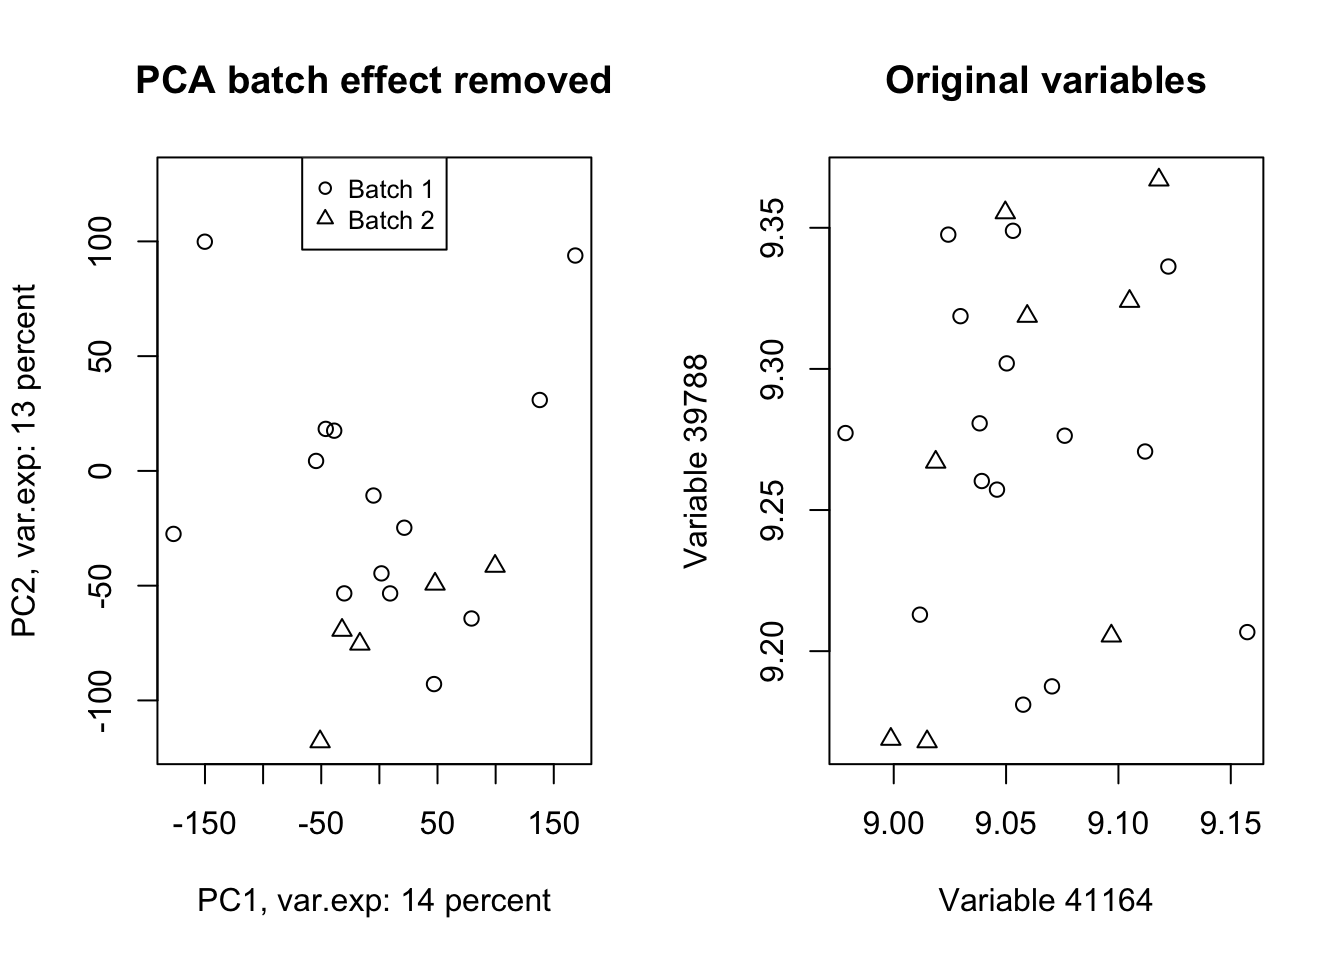
\includegraphics{PCA_files/figure-latex/pcabatch2-1} 

}

\caption{PCA of the data showing the removal of batch effect in our data}\label{fig:pcabatch2}
\end{figure}

Isn't this beautiful!? What we did in this plot (Figure \ref{fig:pcabatch2} ) was rebuilding (called reconstruction) of our data without the variation that we are not interested in and did another PCA to check where most of the variation is in the new data (the plot on the left)! We also plotted the same variables that we plotted in Figure \ref{fig:pcabatch1}. We clearly see that the batch effect has gone. We can use the very same method to remove/keep any variation or data pattern. We can also use the same method to decrease the size of images etc etc.

That was it for the application PCA. We are going to do some simple exercises in \protect\hyperlink{exer}{the next chapter} and then jump into \protect\hyperlink{pcamath}{the mathematical} details of PCA.

\hypertarget{exer}{%
\chapter{Exercises}\label{exer}}

Welcome to the exercises! We are going to do three exercises based on a dataset that is already available in you R environment. We are not providing answer to the exercises. You will have to find them yourself.

\hypertarget{data}{%
\section{Data}\label{data}}

The dataset is called \emph{iris}. It's coming default with R. According to R help page this is:

\begin{verbatim}
This famous (Fisher's or Anderson's) iris data set gives the measurements in centimeters of the variables sepal length and width and petal length and width, respectively, for 50 flowers from each of 3 species of iris. The species are Iris setosa, versicolor, and virginic
\end{verbatim}

You can simply write iris in your R console to make sure you have the dataset. If you see an error, try

\begin{verbatim}
data(iris)
\end{verbatim}

The dataset contains 5 columns corresponding to four variables and one grouping information.

PCA only works on the numberical data. You can extract the four numerical variables using

\begin{verbatim}
iris[,1:4]
\end{verbatim}

The grouping information can be extracted using

\begin{verbatim}
iris[,5]
\end{verbatim}

Now you have all you need!

\hypertarget{exercise-1}{%
\section{Exercise 1}\label{exercise-1}}

How does the data look? Do you see any pattern!? Any differences between groups?

Produce a plot showing the differences between the groups. You will have to do a pca and make a plot of PCA scores (components)

\hypertarget{exercise-2}{%
\section{Exercise 2}\label{exercise-2}}

What is the most important variable in component 4? What does it show? What is the meaning of it?

\hypertarget{exercise-3}{%
\section{Exercise 3}\label{exercise-3}}

What is the most important variable affected by the species of lowers?

\hypertarget{exercise-4}{%
\section{Exercise 4}\label{exercise-4}}

Remove the first component and reconstruct the data. Now repeat exercises 1 to 3!

Goog luck!

\hypertarget{pcamath}{%
\chapter{PCA (mathematical details)}\label{pcamath}}

Welcome to the last section of this chapter. We are going to talk a bit about the mathematical details of PCA. It's important that, it's not necessary to understand the mathematical details of PCA in order to effectively apply this amazing method on your data. One can easily skip this section without having any problems when it comes to the application. So feel free to skip this if you find difficult to follow!

\hypertarget{summary-of-the-previous-chapter-2}{%
\section{Summary of the previous chapter}\label{summary-of-the-previous-chapter-2}}

Since the beginning of this chapter, we have been talking about variance as a measure of variability in our data. We also talked a bit about covariance as a measure of concordance or redundancy in our data (or even total variance). We saw that working with high dimensional data is challenging and PCA can help us summarize these dimensions (e.g.~genes) into a set of new variables (scores/components) so that one we see the pattern of data spread. The new dimensions were promised to be orthogonal (no covariance) and sorted so that the variance of the first variable is always higher than the second one and so on. We are now ready to see how PCA does this amazing calculation.

\hypertarget{foundations}{%
\section{Foundations}\label{foundations}}

In order to understand the math behind PCA, we need to agree on a set of definitions.

\begin{definition}[Scalar]
\protect\hypertarget{def:scalar}{}{\label{def:scalar} \iffalse (Scalar) \fi{} }A scalar is a number. We work a lot with scalars. For example age,speed, temperature etc. Of course, scalars can have signs (positive and negative) and we can add them, subtract them, multiply etc.
\end{definition}

\begin{definition}[Space]
\protect\hypertarget{def:space}{}{\label{def:space} \iffalse (Space) \fi{} }This might sound a bit tricky to understand. In fact the meaning of space can be very complicated.
In our case, we define the space of a dataset to be the set of all variables defining the dimensions
of the space and their \textbf{possible} values define the extend of the space. In math we define space
by \({\rm I\!R}^n\) or \({\rm I\!E}^n\) where ``n'' means the number of dimentions.
\end{definition}

For example in our data, we have n=45101 that is equal to the number of genes we have measured, meaning that the space our data has 45101 dimensions. You can think about the extend of these dimensions to be all possible expression of each genes. For example, if we only have two genes in our data, we have \({\rm I\!R}^2\) giving us a 2 dimensional space. The size of this space starts from the lowest possible value for the expression of the genes to the highest possible value. The exact measured expression of each gene gives us the location of our observation in the space.

\begin{Shaded}
\begin{Highlighting}[]
\CommentTok{# Select variable}
\NormalTok{var1<-}\DecValTok{18924}
\NormalTok{var3<-}\DecValTok{18505}
\CommentTok{# plot the data for variable 1}
\KeywordTok{plot}\NormalTok{(data[,}\KeywordTok{c}\NormalTok{(var1,var3)],}\DataTypeTok{xlab =} \StringTok{"Variable 1"}\NormalTok{,}\DataTypeTok{ylab =} \StringTok{"Variable 2"}\NormalTok{,}
     \DataTypeTok{ylim =} \KeywordTok{c}\NormalTok{(}\DecValTok{0}\NormalTok{,}\DecValTok{15}\NormalTok{),}\DataTypeTok{xlim=}\KeywordTok{c}\NormalTok{(}\DecValTok{0}\NormalTok{,}\DecValTok{20}\NormalTok{))}
\end{Highlighting}
\end{Shaded}

\begin{figure}

{\centering 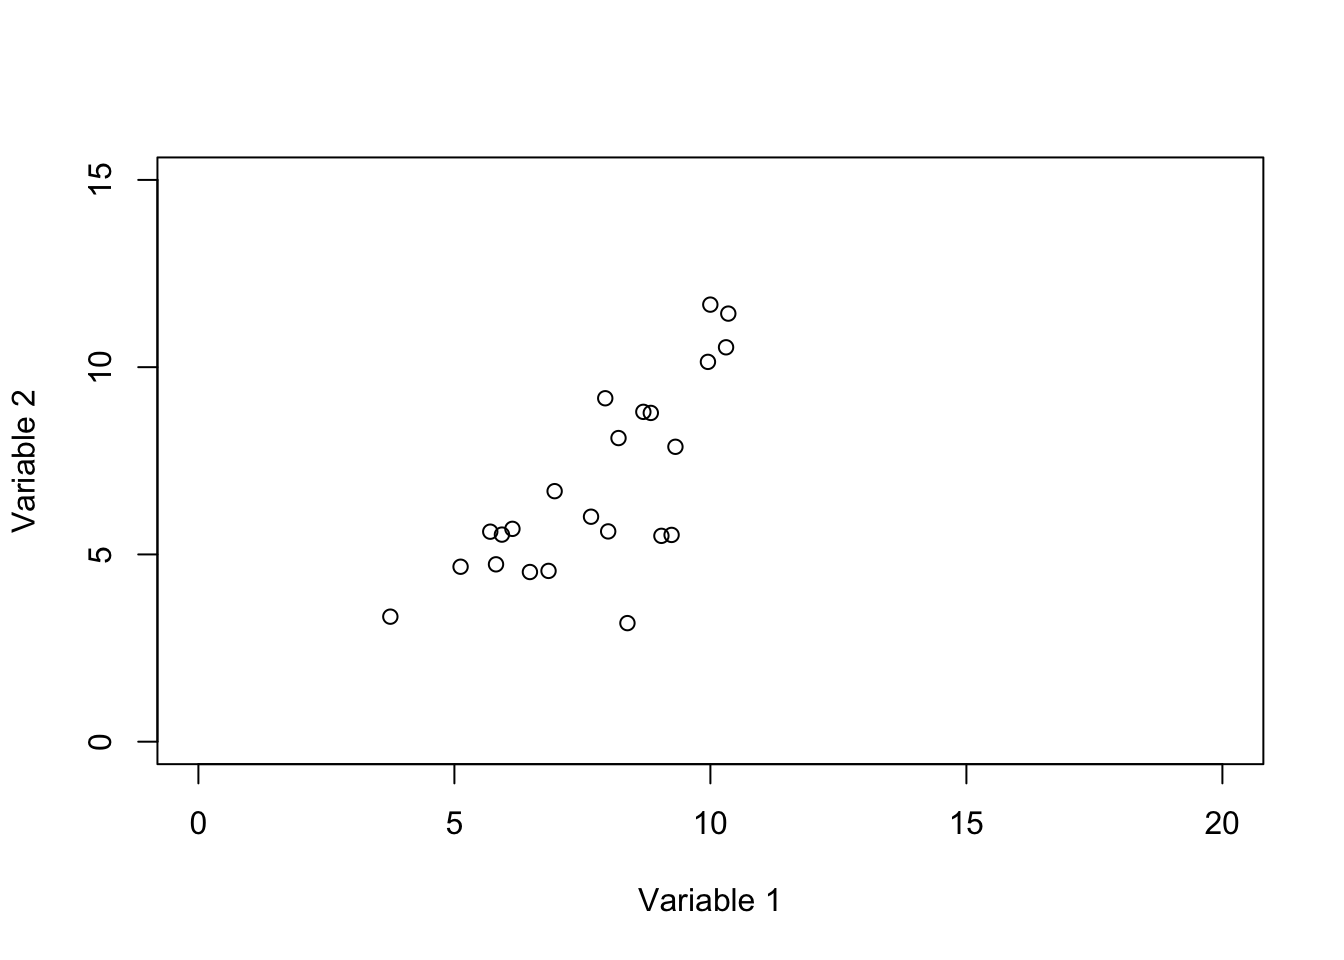
\includegraphics{PCA_files/figure-latex/spaceex1-1} 

}

\caption{Plot of two genes showing the space defined by these two variables}\label{fig:spaceex1}
\end{figure}

In Figure \ref{fig:spaceex1} we show two variables. the value of \emph{variable 1} start from 0 and go all the way to 20 whereas the value of \emph{variable 2} starts from 0 and go to 15. So to put it in context, our space is defined by these variable and their possible values. Our observations (e.g.~samples) are just some points or location in that space. However, for simplicity, we limit the extend of the values to the ones that we observed in our data and not all possible values of variable 1 and 2.

Another way of thinking about the space is imagine \emph{outer space} which more or less defines what exists in the universe and planets, stars and in general celestial bodies are located somewhere in the space.

\begin{Shaded}
\begin{Highlighting}[]
\NormalTok{knitr}\OperatorTok{::}\KeywordTok{include_graphics}\NormalTok{(}\KeywordTok{rep}\NormalTok{(}\StringTok{'https://www.jpl.nasa.gov/spaceimages/images/wallpaper/PIA22564-640x350.jpg'}\NormalTok{))}
\end{Highlighting}
\end{Shaded}

\begin{center}\includegraphics{https://www.jpl.nasa.gov/spaceimages/images/wallpaper/PIA22564-640x350} \end{center}

\begin{definition}[Origin]
\protect\hypertarget{def:origin}{}{\label{def:origin} \iffalse (Origin) \fi{} }Let's agree that the start of everything is from zero (0). Formally the location where axis of our space intersect is zero. Another way of thinking about this is if you multiple anything by zero the result will be zero! This is normally denoted by \((0,0)\) or sometime just \(O\).
\end{definition}

\begin{Shaded}
\begin{Highlighting}[]
\CommentTok{# plot the data for variable 1}
\KeywordTok{plot}\NormalTok{(}\KeywordTok{c}\NormalTok{(}\OperatorTok{-}\DecValTok{2}\NormalTok{,}\DecValTok{2}\NormalTok{),}\KeywordTok{c}\NormalTok{(}\OperatorTok{-}\DecValTok{2}\NormalTok{,}\DecValTok{2}\NormalTok{),}\DataTypeTok{xlab =} \StringTok{""}\NormalTok{,}\DataTypeTok{ylab =} \StringTok{""}\NormalTok{,}
 \DataTypeTok{axes =}\NormalTok{ F,}\DataTypeTok{type =} \StringTok{"n"}\NormalTok{)}

\CommentTok{# plot the axis}
\KeywordTok{axis}\NormalTok{(}\DecValTok{1}\NormalTok{,}\DataTypeTok{cex=}\DecValTok{4}\NormalTok{,}\DataTypeTok{pos =} \KeywordTok{c}\NormalTok{(}\DecValTok{0}\NormalTok{,}\DecValTok{0}\NormalTok{) )}
\KeywordTok{axis}\NormalTok{(}\DecValTok{2}\NormalTok{,}\DataTypeTok{cex=}\DecValTok{4}\NormalTok{,}\DataTypeTok{pos =} \KeywordTok{c}\NormalTok{(}\DecValTok{0}\NormalTok{,}\DecValTok{0}\NormalTok{) )}

\CommentTok{# plot arrow and text}
\KeywordTok{arrows}\NormalTok{(}\DecValTok{1}\NormalTok{,}\DecValTok{1}\NormalTok{,}\DecValTok{0}\NormalTok{,}\DecValTok{0}\NormalTok{)}
\KeywordTok{text}\NormalTok{(}\KeywordTok{c}\NormalTok{(}\FloatTok{1.1}\NormalTok{),}\DataTypeTok{label =} \StringTok{"Origin (0,0)"}\NormalTok{)}
\end{Highlighting}
\end{Shaded}

\begin{figure}

{\centering 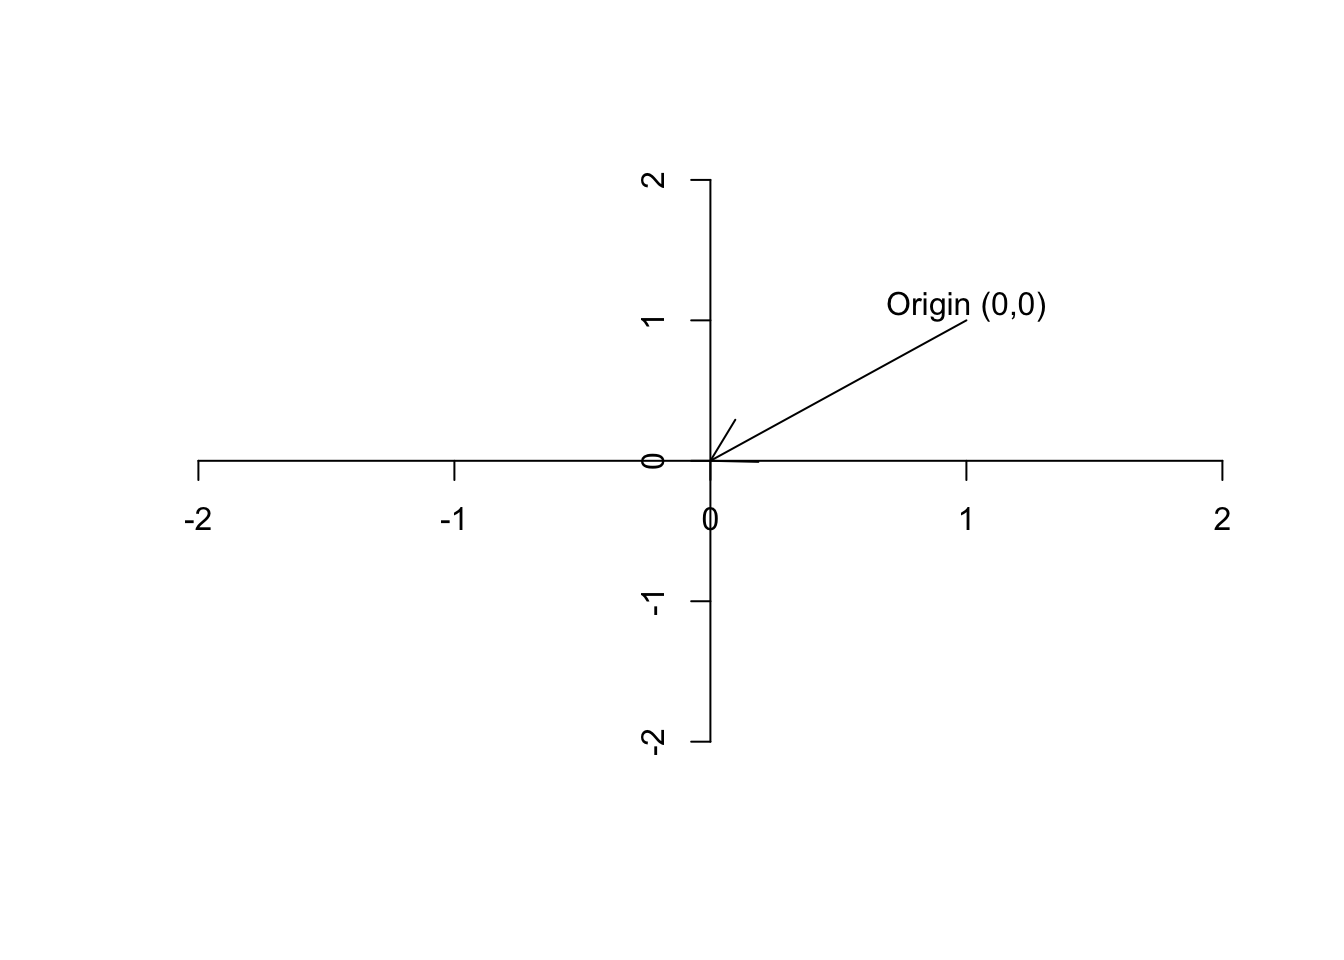
\includegraphics{PCA_files/figure-latex/spaceex2-1} 

}

\caption{Plot of the origin}\label{fig:spaceex2}
\end{figure}

\begin{definition}[Vector]
\protect\hypertarget{def:vectors}{}{\label{def:vectors} \iffalse (Vector) \fi{} }A vector is basically just a list of numbers, showing a location of a point in the space. We like to show the vectors by their name and a small arrow on top of them (\(\vec{a}\)). For example, if we say \(\vec{a}=[5,13]\), it means we are refering to a point in space where the value for the first axis is 2 and the second axis is 13. It's often nice to show the vector with an arrow starting from the origin and finishing exactly at that point.
\end{definition}

\begin{Shaded}
\begin{Highlighting}[]
\CommentTok{# plot the data for variable 1}
\KeywordTok{plot}\NormalTok{(}\KeywordTok{c}\NormalTok{(}\OperatorTok{-}\DecValTok{20}\NormalTok{,}\DecValTok{20}\NormalTok{),}\KeywordTok{c}\NormalTok{(}\OperatorTok{-}\DecValTok{20}\NormalTok{,}\DecValTok{20}\NormalTok{),}\DataTypeTok{xlab =} \StringTok{""}\NormalTok{,}\DataTypeTok{ylab =} \StringTok{""}\NormalTok{,}
 \DataTypeTok{axes =}\NormalTok{ F,}\DataTypeTok{type =} \StringTok{"n"}\NormalTok{)}

\CommentTok{# plot the point}
\KeywordTok{points}\NormalTok{(}\DecValTok{5}\NormalTok{,}\DecValTok{13}\NormalTok{)}
\CommentTok{# plot the axis}
\KeywordTok{axis}\NormalTok{(}\DecValTok{1}\NormalTok{,}\DataTypeTok{cex=}\DecValTok{4}\NormalTok{,}\DataTypeTok{pos =} \KeywordTok{c}\NormalTok{(}\DecValTok{0}\NormalTok{,}\DecValTok{0}\NormalTok{) )}
\KeywordTok{title}\NormalTok{(}\DataTypeTok{xlab=}\StringTok{"x"}\NormalTok{, }\DataTypeTok{line=}\OperatorTok{-}\DecValTok{10}\NormalTok{, }\DataTypeTok{cex.lab=}\FloatTok{1.2}\NormalTok{,}\DataTypeTok{adj=}\DecValTok{1}\NormalTok{)}
\KeywordTok{axis}\NormalTok{(}\DecValTok{2}\NormalTok{,}\DataTypeTok{cex=}\DecValTok{4}\NormalTok{,}\DataTypeTok{pos =} \KeywordTok{c}\NormalTok{(}\DecValTok{0}\NormalTok{,}\DecValTok{0}\NormalTok{) )}
\KeywordTok{title}\NormalTok{(}\DataTypeTok{ylab=}\StringTok{"y"}\NormalTok{, }\DataTypeTok{line=}\OperatorTok{-}\DecValTok{17}\NormalTok{, }\DataTypeTok{cex.lab=}\FloatTok{1.2}\NormalTok{,}\DataTypeTok{adj=}\DecValTok{1}\NormalTok{)}
\CommentTok{# plot arrow and text}
\KeywordTok{arrows}\NormalTok{(}\DecValTok{0}\NormalTok{,}\DecValTok{0}\NormalTok{,}\DecValTok{5}\NormalTok{,}\DecValTok{13}\NormalTok{)}
\end{Highlighting}
\end{Shaded}

\begin{figure}

{\centering 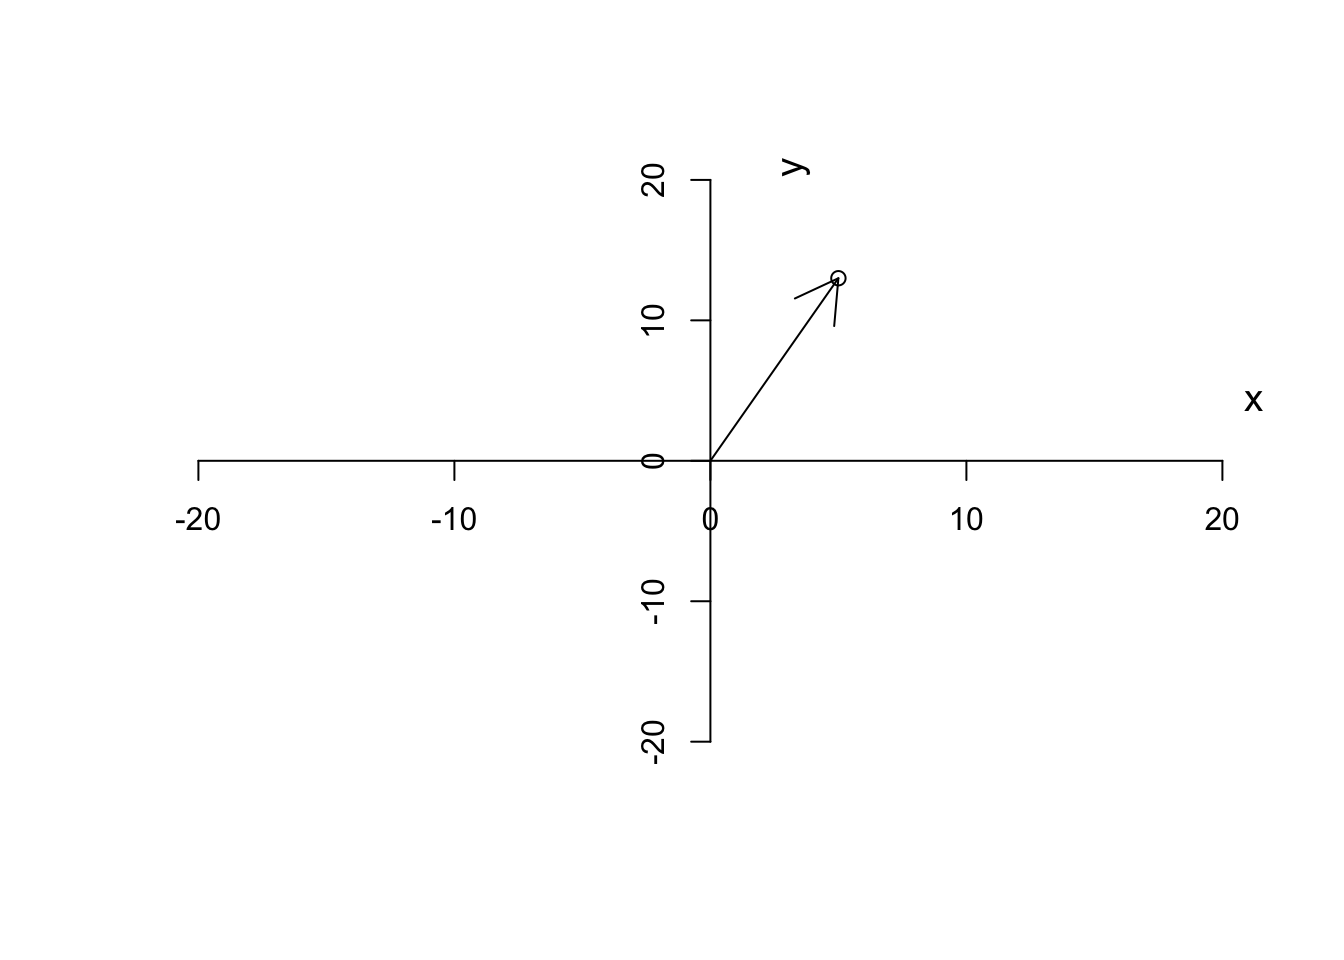
\includegraphics{PCA_files/figure-latex/spaceex3-1} 

}

\caption{Plotting a vector}\label{fig:spaceex3}
\end{figure}

As we said, we like to put our starting point at \((0,0)\). Given this, we can also think about a vector as magnitude (length the arrow starting from the origin or distance to the origin) and also the direction to which the arrow is pointing.
So in \protect\hyperlink{spaceex3}{our case}, we have a vector that is defined by going to the right along the \(x\) axis (red arrow in Figure \ref{fig:spaceex4}) until reaching point 3 and the start going up along the \(y\) axis (blue arrow in Figure \ref{fig:spaceex4}) to reach the final point.

\begin{Shaded}
\begin{Highlighting}[]
\CommentTok{# plot the data for variable 1}
\KeywordTok{plot}\NormalTok{(}\KeywordTok{c}\NormalTok{(}\OperatorTok{-}\DecValTok{20}\NormalTok{,}\DecValTok{20}\NormalTok{),}\KeywordTok{c}\NormalTok{(}\OperatorTok{-}\DecValTok{20}\NormalTok{,}\DecValTok{20}\NormalTok{),}\DataTypeTok{xlab =} \StringTok{""}\NormalTok{,}\DataTypeTok{ylab =} \StringTok{""}\NormalTok{,}
 \DataTypeTok{axes =}\NormalTok{ F,}\DataTypeTok{type =} \StringTok{"n"}\NormalTok{)}

\CommentTok{# plot the point}
\KeywordTok{points}\NormalTok{(}\DecValTok{5}\NormalTok{,}\DecValTok{13}\NormalTok{)}
\CommentTok{# plot the axis}
\KeywordTok{axis}\NormalTok{(}\DecValTok{1}\NormalTok{,}\DataTypeTok{cex=}\DecValTok{4}\NormalTok{,}\DataTypeTok{pos =} \KeywordTok{c}\NormalTok{(}\DecValTok{0}\NormalTok{,}\DecValTok{0}\NormalTok{) )}
\KeywordTok{title}\NormalTok{(}\DataTypeTok{xlab=}\StringTok{"x"}\NormalTok{, }\DataTypeTok{line=}\OperatorTok{-}\DecValTok{10}\NormalTok{, }\DataTypeTok{cex.lab=}\FloatTok{1.2}\NormalTok{,}\DataTypeTok{adj=}\DecValTok{1}\NormalTok{)}
\KeywordTok{axis}\NormalTok{(}\DecValTok{2}\NormalTok{,}\DataTypeTok{cex=}\DecValTok{4}\NormalTok{,}\DataTypeTok{pos =} \KeywordTok{c}\NormalTok{(}\DecValTok{0}\NormalTok{,}\DecValTok{0}\NormalTok{) )}
\KeywordTok{title}\NormalTok{(}\DataTypeTok{ylab=}\StringTok{"y"}\NormalTok{, }\DataTypeTok{line=}\OperatorTok{-}\DecValTok{16}\NormalTok{, }\DataTypeTok{cex.lab=}\FloatTok{1.2}\NormalTok{,}\DataTypeTok{adj=}\DecValTok{1}\NormalTok{)}
\CommentTok{# plot arrow and text}
\KeywordTok{arrows}\NormalTok{(}\DecValTok{0}\NormalTok{,}\DecValTok{0}\NormalTok{,}\DecValTok{5}\NormalTok{,}\DecValTok{13}\NormalTok{)}

\KeywordTok{arrows}\NormalTok{(}\DecValTok{0}\NormalTok{,}\DecValTok{0}\NormalTok{,}\DecValTok{5}\NormalTok{,}\DecValTok{0}\NormalTok{,}\DataTypeTok{col=}\StringTok{"Red"}\NormalTok{,}\DataTypeTok{lty =} \StringTok{"dashed"}\NormalTok{)}
\KeywordTok{arrows}\NormalTok{(}\DecValTok{5}\NormalTok{,}\DecValTok{0}\NormalTok{,}\DecValTok{5}\NormalTok{,}\DecValTok{13}\NormalTok{,}\DataTypeTok{col=}\StringTok{"blue"}\NormalTok{,}\DataTypeTok{lty =} \StringTok{"dashed"}\NormalTok{)}
\end{Highlighting}
\end{Shaded}

\begin{figure}

{\centering 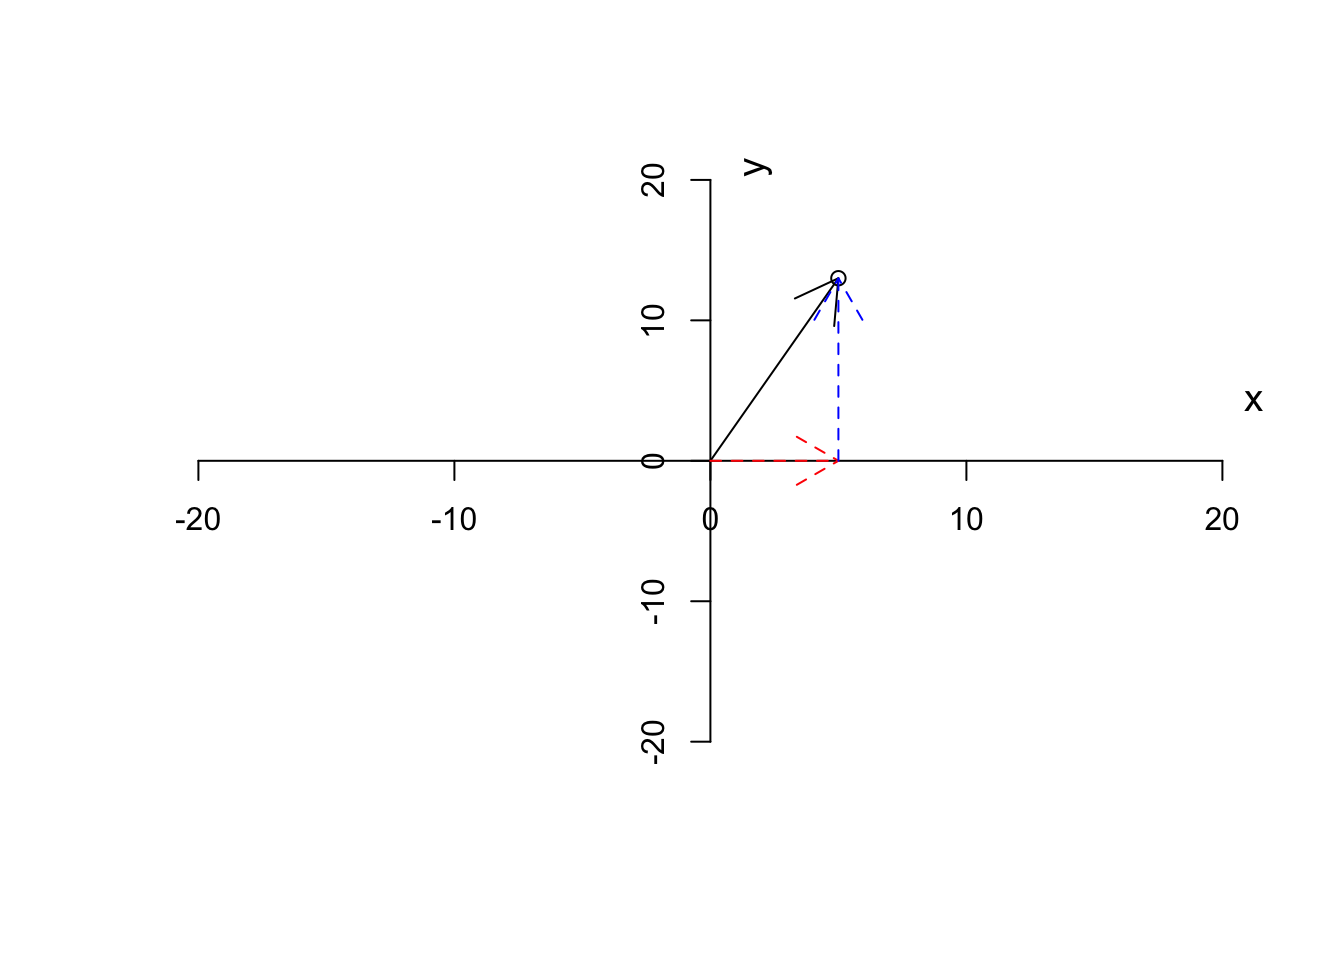
\includegraphics{PCA_files/figure-latex/spaceex4-1} 

}

\caption{Plotting a vector and the steps}\label{fig:spaceex4}
\end{figure}

The magnitude of a vector is calculated by:

\[\|\vec{a}\|=\sqrt{x^2+y^2}\]
Where \(x\) and \(y\) are the first and the second elements of the vector. So in our case that is equal to \(\|\vec{a}\|=\sqrt{5^2+13^2}=13.93\).

We normally like to measure the direction of the a vector based on the angle it makes with the \(x\) axis.

\[\theta=\tan^{-1}\frac{x}{y}\]
These thing can easily be calculate in R for example by

\begin{verbatim}
atan(y/x)
\end{verbatim}

\begin{Shaded}
\begin{Highlighting}[]
\CommentTok{# plot the data for variable 1}
\KeywordTok{plot}\NormalTok{(}\KeywordTok{c}\NormalTok{(}\OperatorTok{-}\DecValTok{20}\NormalTok{,}\DecValTok{20}\NormalTok{),}\KeywordTok{c}\NormalTok{(}\OperatorTok{-}\DecValTok{20}\NormalTok{,}\DecValTok{20}\NormalTok{),}\DataTypeTok{xlab =} \StringTok{""}\NormalTok{,}\DataTypeTok{ylab =} \StringTok{""}\NormalTok{,}
 \DataTypeTok{axes =}\NormalTok{ F,}\DataTypeTok{type =} \StringTok{"n"}\NormalTok{)}

\CommentTok{# plot the point}
\KeywordTok{points}\NormalTok{(}\DecValTok{5}\NormalTok{,}\DecValTok{13}\NormalTok{)}
\CommentTok{# plot the axis}
\KeywordTok{axis}\NormalTok{(}\DecValTok{1}\NormalTok{,}\DataTypeTok{cex=}\DecValTok{4}\NormalTok{,}\DataTypeTok{pos =} \KeywordTok{c}\NormalTok{(}\DecValTok{0}\NormalTok{,}\DecValTok{0}\NormalTok{) )}
\KeywordTok{title}\NormalTok{(}\DataTypeTok{xlab=}\StringTok{"x"}\NormalTok{, }\DataTypeTok{line=}\OperatorTok{-}\DecValTok{10}\NormalTok{, }\DataTypeTok{cex.lab=}\FloatTok{1.2}\NormalTok{,}\DataTypeTok{adj=}\DecValTok{1}\NormalTok{)}
\KeywordTok{axis}\NormalTok{(}\DecValTok{2}\NormalTok{,}\DataTypeTok{cex=}\DecValTok{4}\NormalTok{,}\DataTypeTok{pos =} \KeywordTok{c}\NormalTok{(}\DecValTok{0}\NormalTok{,}\DecValTok{0}\NormalTok{) )}
\KeywordTok{title}\NormalTok{(}\DataTypeTok{ylab=}\StringTok{"y"}\NormalTok{, }\DataTypeTok{line=}\OperatorTok{-}\DecValTok{16}\NormalTok{, }\DataTypeTok{cex.lab=}\FloatTok{1.2}\NormalTok{,}\DataTypeTok{adj=}\DecValTok{1}\NormalTok{)}
\CommentTok{# plot arrow and text}
\KeywordTok{arrows}\NormalTok{(}\DecValTok{0}\NormalTok{,}\DecValTok{0}\NormalTok{,}\DecValTok{5}\NormalTok{,}\DecValTok{13}\NormalTok{)}

\CommentTok{# draw arc}
\NormalTok{plotrix}\OperatorTok{::}\KeywordTok{draw.arc}\NormalTok{(}\DecValTok{0}\NormalTok{,}\DecValTok{0}\NormalTok{,}\DecValTok{3}\NormalTok{,}\DataTypeTok{angle2=}\DecValTok{1}\NormalTok{)}

\KeywordTok{text}\NormalTok{(}\DecValTok{1}\NormalTok{,}\DecValTok{1}\NormalTok{,}\StringTok{"1.2"}\NormalTok{,}\DataTypeTok{cex=}\FloatTok{0.7}\NormalTok{)}
\end{Highlighting}
\end{Shaded}

\begin{figure}

{\centering 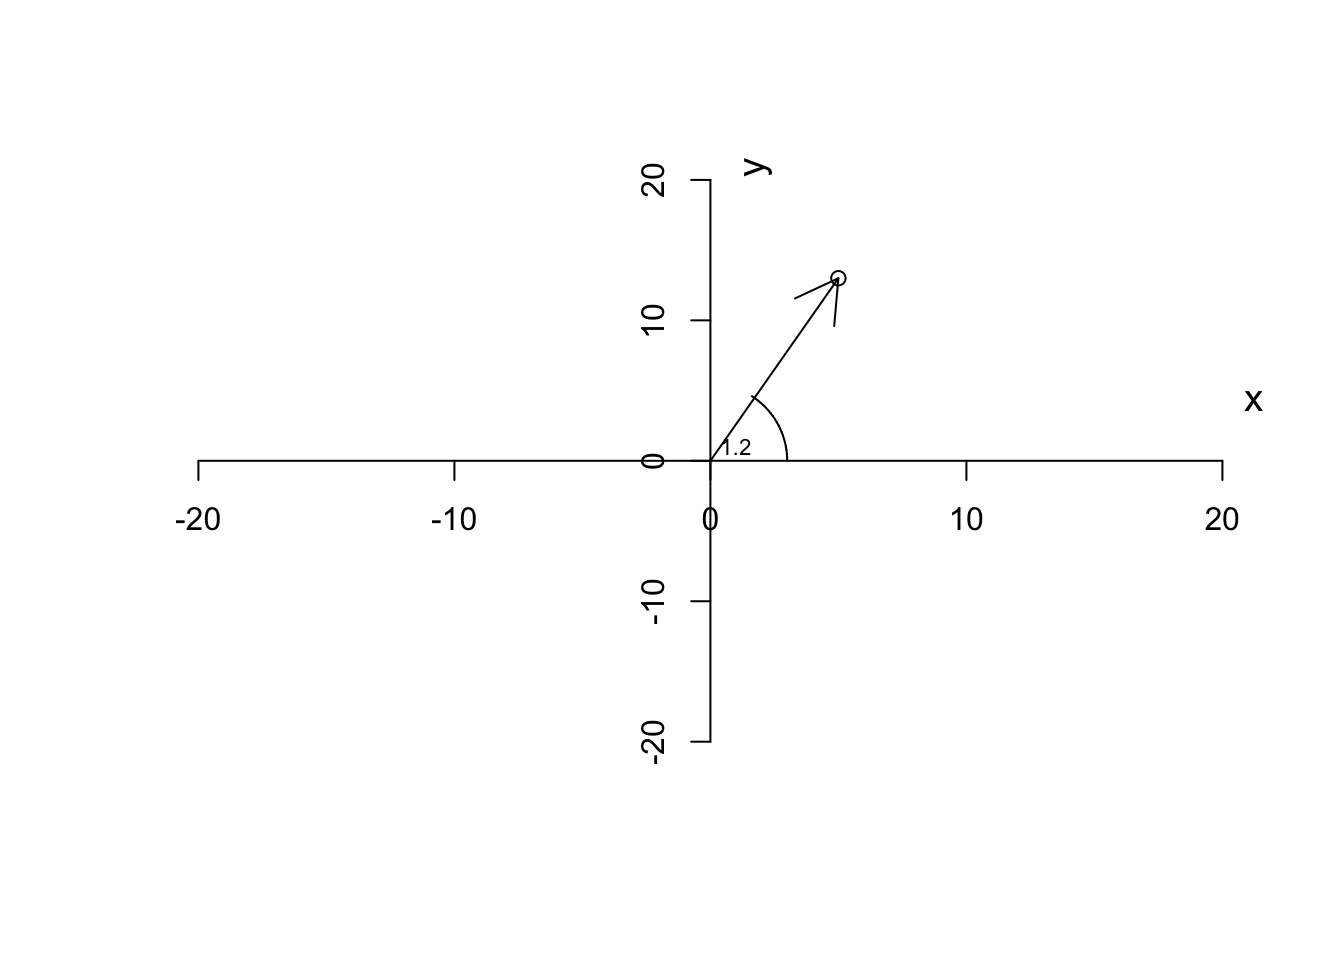
\includegraphics{PCA_files/figure-latex/spaceex5-1} 

}

\caption{Plotting a vector and the steps}\label{fig:spaceex5}
\end{figure}

So by now we have the magnitude and direction of a vector. A vector also has a span. A span of a vector is a line resulted by stretching the vector from both ends to infinity.

\begin{Shaded}
\begin{Highlighting}[]
\CommentTok{# plot the data for variable 1}
\KeywordTok{plot}\NormalTok{(}\KeywordTok{c}\NormalTok{(}\OperatorTok{-}\DecValTok{20}\NormalTok{,}\DecValTok{20}\NormalTok{),}\KeywordTok{c}\NormalTok{(}\OperatorTok{-}\DecValTok{20}\NormalTok{,}\DecValTok{20}\NormalTok{),}\DataTypeTok{xlab =} \StringTok{""}\NormalTok{,}\DataTypeTok{ylab =} \StringTok{""}\NormalTok{,}
 \DataTypeTok{axes =}\NormalTok{ F,}\DataTypeTok{type =} \StringTok{"n"}\NormalTok{)}

\KeywordTok{segments}\NormalTok{(}\OperatorTok{-}\DecValTok{500}\NormalTok{,}\OperatorTok{-}\DecValTok{1300}\NormalTok{,}\DecValTok{500}\NormalTok{,}\DecValTok{1300}\NormalTok{,}\DataTypeTok{col =} \StringTok{"red"}\NormalTok{,}\DataTypeTok{lty =} \StringTok{"dashed"}\NormalTok{)}
\KeywordTok{text}\NormalTok{(}\DecValTok{13}\NormalTok{,}\DecValTok{20}\NormalTok{,}\StringTok{"span of the vector"}\NormalTok{,}\DataTypeTok{col=}\StringTok{"red"}\NormalTok{)}
\CommentTok{# plot the point}
\KeywordTok{points}\NormalTok{(}\DecValTok{5}\NormalTok{,}\DecValTok{13}\NormalTok{)}
\CommentTok{# plot the axis}
\KeywordTok{axis}\NormalTok{(}\DecValTok{1}\NormalTok{,}\DataTypeTok{cex=}\DecValTok{4}\NormalTok{,}\DataTypeTok{pos =} \KeywordTok{c}\NormalTok{(}\DecValTok{0}\NormalTok{,}\DecValTok{0}\NormalTok{) )}
\KeywordTok{title}\NormalTok{(}\DataTypeTok{xlab=}\StringTok{"x"}\NormalTok{, }\DataTypeTok{line=}\OperatorTok{-}\DecValTok{10}\NormalTok{, }\DataTypeTok{cex.lab=}\FloatTok{1.2}\NormalTok{,}\DataTypeTok{adj=}\DecValTok{1}\NormalTok{)}
\KeywordTok{axis}\NormalTok{(}\DecValTok{2}\NormalTok{,}\DataTypeTok{cex=}\DecValTok{4}\NormalTok{,}\DataTypeTok{pos =} \KeywordTok{c}\NormalTok{(}\DecValTok{0}\NormalTok{,}\DecValTok{0}\NormalTok{) )}
\KeywordTok{title}\NormalTok{(}\DataTypeTok{ylab=}\StringTok{"y"}\NormalTok{, }\DataTypeTok{line=}\OperatorTok{-}\DecValTok{16}\NormalTok{, }\DataTypeTok{cex.lab=}\FloatTok{1.2}\NormalTok{,}\DataTypeTok{adj=}\DecValTok{1}\NormalTok{)}
\CommentTok{# plot arrow and text}
\KeywordTok{arrows}\NormalTok{(}\DecValTok{0}\NormalTok{,}\DecValTok{0}\NormalTok{,}\DecValTok{5}\NormalTok{,}\DecValTok{13}\NormalTok{)}
\CommentTok{# draw circle}
\NormalTok{plotrix}\OperatorTok{::}\KeywordTok{draw.arc}\NormalTok{(}\DecValTok{0}\NormalTok{,}\DecValTok{0}\NormalTok{,}\DecValTok{3}\NormalTok{,}\DataTypeTok{angle2=}\DecValTok{1}\NormalTok{)}

\KeywordTok{text}\NormalTok{(}\DecValTok{1}\NormalTok{,}\DecValTok{1}\NormalTok{,}\StringTok{"1.2"}\NormalTok{,}\DataTypeTok{cex=}\FloatTok{0.7}\NormalTok{)}
\end{Highlighting}
\end{Shaded}

\begin{figure}

{\centering 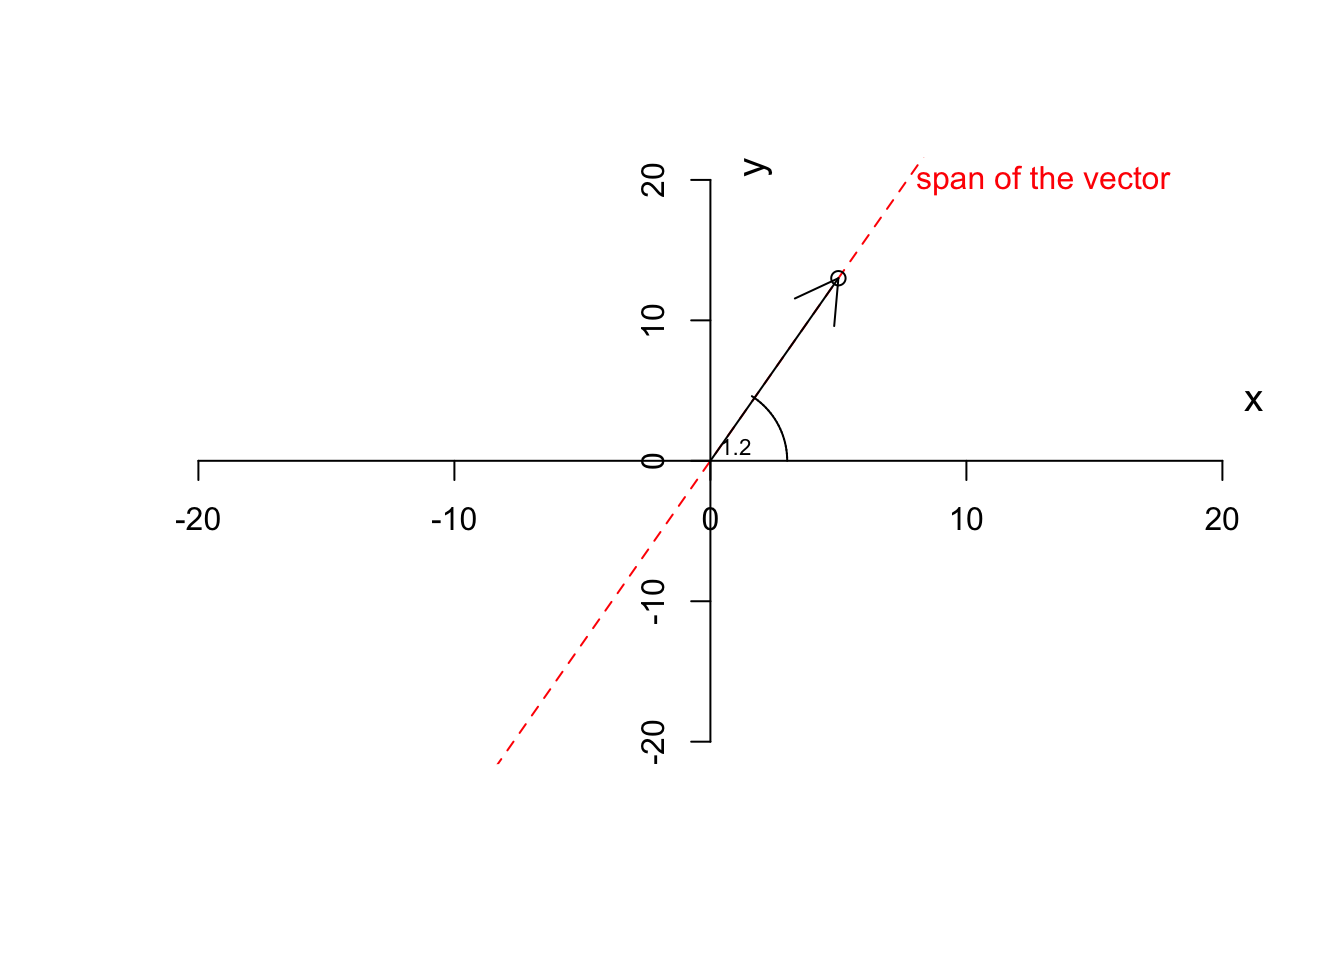
\includegraphics{PCA_files/figure-latex/spaceex6-1} 

}

\caption{Plotting a vector and the steps}\label{fig:spaceex6}
\end{figure}

Now we can go ahead and define some preliminary operations on the vector.

\hypertarget{operations-on-vectors}{%
\section{Operations on vectors}\label{operations-on-vectors}}

\begin{definition}[Scalar multiplication]
\protect\hypertarget{def:scalarv}{}{\label{def:scalarv} \iffalse (Scalar multiplication) \fi{} }If we multiply a vector by a scalar (a number) other than one (1), the resulting vector will change magnitunde by not direction. However, a vector might flip (pointing to opposite direction) but it will NEVER change the direction of its span.

When we multiply a scalar to a vector, we take each element of the vector (e.g.~\(x\) and \(y\)) and we multiply each of them by that scalar

\[\vec{a} \times j=[x\times j,y\times j]\]

where \(\vec{a}\) is a vector and \(j\) is an scalar.
\end{definition}

For example if we take our vector \(\vec{a}=[5,13]\) and multiply by \(1.5\) the results will be \([5 \times 1.5, 13 \times 1.5]=[7.5,19.5]\):

\begin{Shaded}
\begin{Highlighting}[]
\CommentTok{# plot the data for variable 1}
\KeywordTok{plot}\NormalTok{(}\KeywordTok{c}\NormalTok{(}\OperatorTok{-}\DecValTok{20}\NormalTok{,}\DecValTok{20}\NormalTok{),}\KeywordTok{c}\NormalTok{(}\OperatorTok{-}\DecValTok{20}\NormalTok{,}\DecValTok{20}\NormalTok{),}\DataTypeTok{xlab =} \StringTok{""}\NormalTok{,}\DataTypeTok{ylab =} \StringTok{""}\NormalTok{,}
 \DataTypeTok{axes =}\NormalTok{ F,}\DataTypeTok{type =} \StringTok{"n"}\NormalTok{)}

\KeywordTok{segments}\NormalTok{(}\OperatorTok{-}\DecValTok{500}\NormalTok{,}\OperatorTok{-}\DecValTok{1300}\NormalTok{,}\DecValTok{500}\NormalTok{,}\DecValTok{1300}\NormalTok{,}\DataTypeTok{col =} \StringTok{"red"}\NormalTok{,}\DataTypeTok{lty =} \StringTok{"dashed"}\NormalTok{)}
\KeywordTok{text}\NormalTok{(}\DecValTok{13}\NormalTok{,}\DecValTok{20}\NormalTok{,}\StringTok{"span of the vector"}\NormalTok{,}\DataTypeTok{col=}\StringTok{"red"}\NormalTok{)}

\CommentTok{# plot the axis}
\KeywordTok{axis}\NormalTok{(}\DecValTok{1}\NormalTok{,}\DataTypeTok{cex=}\DecValTok{4}\NormalTok{,}\DataTypeTok{pos =} \KeywordTok{c}\NormalTok{(}\DecValTok{0}\NormalTok{,}\DecValTok{0}\NormalTok{) )}
\KeywordTok{title}\NormalTok{(}\DataTypeTok{xlab=}\StringTok{"x"}\NormalTok{, }\DataTypeTok{line=}\OperatorTok{-}\DecValTok{10}\NormalTok{, }\DataTypeTok{cex.lab=}\FloatTok{1.2}\NormalTok{,}\DataTypeTok{adj=}\DecValTok{1}\NormalTok{)}
\KeywordTok{axis}\NormalTok{(}\DecValTok{2}\NormalTok{,}\DataTypeTok{cex=}\DecValTok{4}\NormalTok{,}\DataTypeTok{pos =} \KeywordTok{c}\NormalTok{(}\DecValTok{0}\NormalTok{,}\DecValTok{0}\NormalTok{) )}
\KeywordTok{title}\NormalTok{(}\DataTypeTok{ylab=}\StringTok{"y"}\NormalTok{, }\DataTypeTok{line=}\OperatorTok{-}\DecValTok{16}\NormalTok{, }\DataTypeTok{cex.lab=}\FloatTok{1.2}\NormalTok{,}\DataTypeTok{adj=}\DecValTok{1}\NormalTok{)}
\CommentTok{# plot arrow and text}

\KeywordTok{arrows}\NormalTok{(}\DecValTok{0}\NormalTok{,}\DecValTok{0}\NormalTok{,}\DecValTok{5}\OperatorTok{*}\FloatTok{1.5}\NormalTok{,}\DecValTok{13}\OperatorTok{*}\FloatTok{1.5}\NormalTok{,}\DataTypeTok{col=}\StringTok{"green"}\NormalTok{)}
\KeywordTok{arrows}\NormalTok{(}\DecValTok{0}\NormalTok{,}\DecValTok{0}\NormalTok{,}\DecValTok{5}\NormalTok{,}\DecValTok{13}\NormalTok{)}

\CommentTok{# draw circle}
\NormalTok{plotrix}\OperatorTok{::}\KeywordTok{draw.arc}\NormalTok{(}\DecValTok{0}\NormalTok{,}\DecValTok{0}\NormalTok{,}\DecValTok{3}\NormalTok{,}\DataTypeTok{angle2=}\DecValTok{1}\NormalTok{)}

\KeywordTok{text}\NormalTok{(}\DecValTok{1}\NormalTok{,}\DecValTok{1}\NormalTok{,}\StringTok{"1.2"}\NormalTok{,}\DataTypeTok{cex=}\FloatTok{0.7}\NormalTok{)}
\end{Highlighting}
\end{Shaded}

\begin{figure}

{\centering 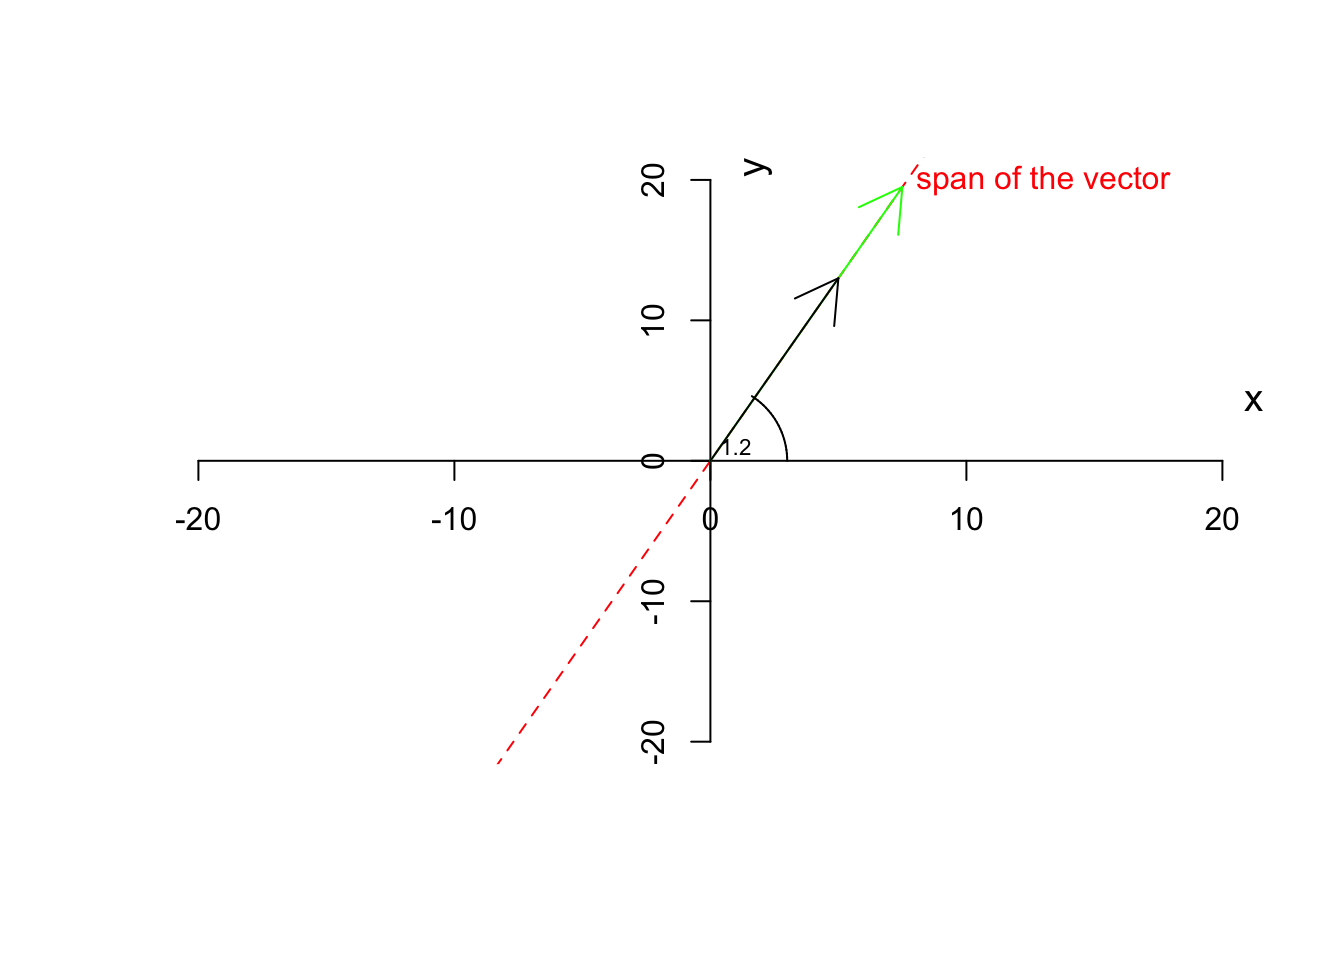
\includegraphics{PCA_files/figure-latex/spaceex7-1} 

}

\caption{Multiplying a vector by a scalar}\label{fig:spaceex7}
\end{figure}

As you see in Figure \ref{fig:spaceex7}, the green vector is the result of the multiplication of the our vector by 1.5. The vector has changed magnitude (length) but not the direction. If we now multiply by \(-1.5\)

\begin{Shaded}
\begin{Highlighting}[]
\CommentTok{# plot the data for variable 1}
\KeywordTok{plot}\NormalTok{(}\KeywordTok{c}\NormalTok{(}\OperatorTok{-}\DecValTok{20}\NormalTok{,}\DecValTok{20}\NormalTok{),}\KeywordTok{c}\NormalTok{(}\OperatorTok{-}\DecValTok{20}\NormalTok{,}\DecValTok{20}\NormalTok{),}\DataTypeTok{xlab =} \StringTok{""}\NormalTok{,}\DataTypeTok{ylab =} \StringTok{""}\NormalTok{,}
 \DataTypeTok{axes =}\NormalTok{ F,}\DataTypeTok{type =} \StringTok{"n"}\NormalTok{)}

\KeywordTok{segments}\NormalTok{(}\OperatorTok{-}\DecValTok{500}\NormalTok{,}\OperatorTok{-}\DecValTok{1300}\NormalTok{,}\DecValTok{500}\NormalTok{,}\DecValTok{1300}\NormalTok{,}\DataTypeTok{col =} \StringTok{"red"}\NormalTok{,}\DataTypeTok{lty =} \StringTok{"dashed"}\NormalTok{)}
\KeywordTok{text}\NormalTok{(}\DecValTok{13}\NormalTok{,}\DecValTok{20}\NormalTok{,}\StringTok{"span of the vector"}\NormalTok{,}\DataTypeTok{col=}\StringTok{"red"}\NormalTok{)}


\CommentTok{# plot the axis}
\KeywordTok{axis}\NormalTok{(}\DecValTok{1}\NormalTok{,}\DataTypeTok{cex=}\DecValTok{4}\NormalTok{,}\DataTypeTok{pos =} \KeywordTok{c}\NormalTok{(}\DecValTok{0}\NormalTok{,}\DecValTok{0}\NormalTok{) )}
\KeywordTok{title}\NormalTok{(}\DataTypeTok{xlab=}\StringTok{"x"}\NormalTok{, }\DataTypeTok{line=}\OperatorTok{-}\DecValTok{10}\NormalTok{, }\DataTypeTok{cex.lab=}\FloatTok{1.2}\NormalTok{,}\DataTypeTok{adj=}\DecValTok{1}\NormalTok{)}
\KeywordTok{axis}\NormalTok{(}\DecValTok{2}\NormalTok{,}\DataTypeTok{cex=}\DecValTok{4}\NormalTok{,}\DataTypeTok{pos =} \KeywordTok{c}\NormalTok{(}\DecValTok{0}\NormalTok{,}\DecValTok{0}\NormalTok{) )}
\KeywordTok{title}\NormalTok{(}\DataTypeTok{ylab=}\StringTok{"y"}\NormalTok{, }\DataTypeTok{line=}\OperatorTok{-}\DecValTok{16}\NormalTok{, }\DataTypeTok{cex.lab=}\FloatTok{1.2}\NormalTok{,}\DataTypeTok{adj=}\DecValTok{1}\NormalTok{)}
\CommentTok{# plot arrow and text}

\KeywordTok{arrows}\NormalTok{(}\DecValTok{0}\NormalTok{,}\DecValTok{0}\NormalTok{,}\DecValTok{5}\OperatorTok{*-}\FloatTok{1.5}\NormalTok{,}\DecValTok{13}\OperatorTok{*-}\FloatTok{1.5}\NormalTok{,}\DataTypeTok{col=}\StringTok{"green"}\NormalTok{)}
\KeywordTok{arrows}\NormalTok{(}\DecValTok{0}\NormalTok{,}\DecValTok{0}\NormalTok{,}\DecValTok{5}\NormalTok{,}\DecValTok{13}\NormalTok{)}

\CommentTok{# draw circle}
\NormalTok{plotrix}\OperatorTok{::}\KeywordTok{draw.arc}\NormalTok{(}\DecValTok{0}\NormalTok{,}\DecValTok{0}\NormalTok{,}\DecValTok{3}\NormalTok{,}\DataTypeTok{angle2=}\DecValTok{1}\NormalTok{)}

\KeywordTok{text}\NormalTok{(}\DecValTok{1}\NormalTok{,}\DecValTok{1}\NormalTok{,}\StringTok{"1.2"}\NormalTok{,}\DataTypeTok{cex=}\FloatTok{0.7}\NormalTok{)}
\end{Highlighting}
\end{Shaded}

\begin{figure}

{\centering 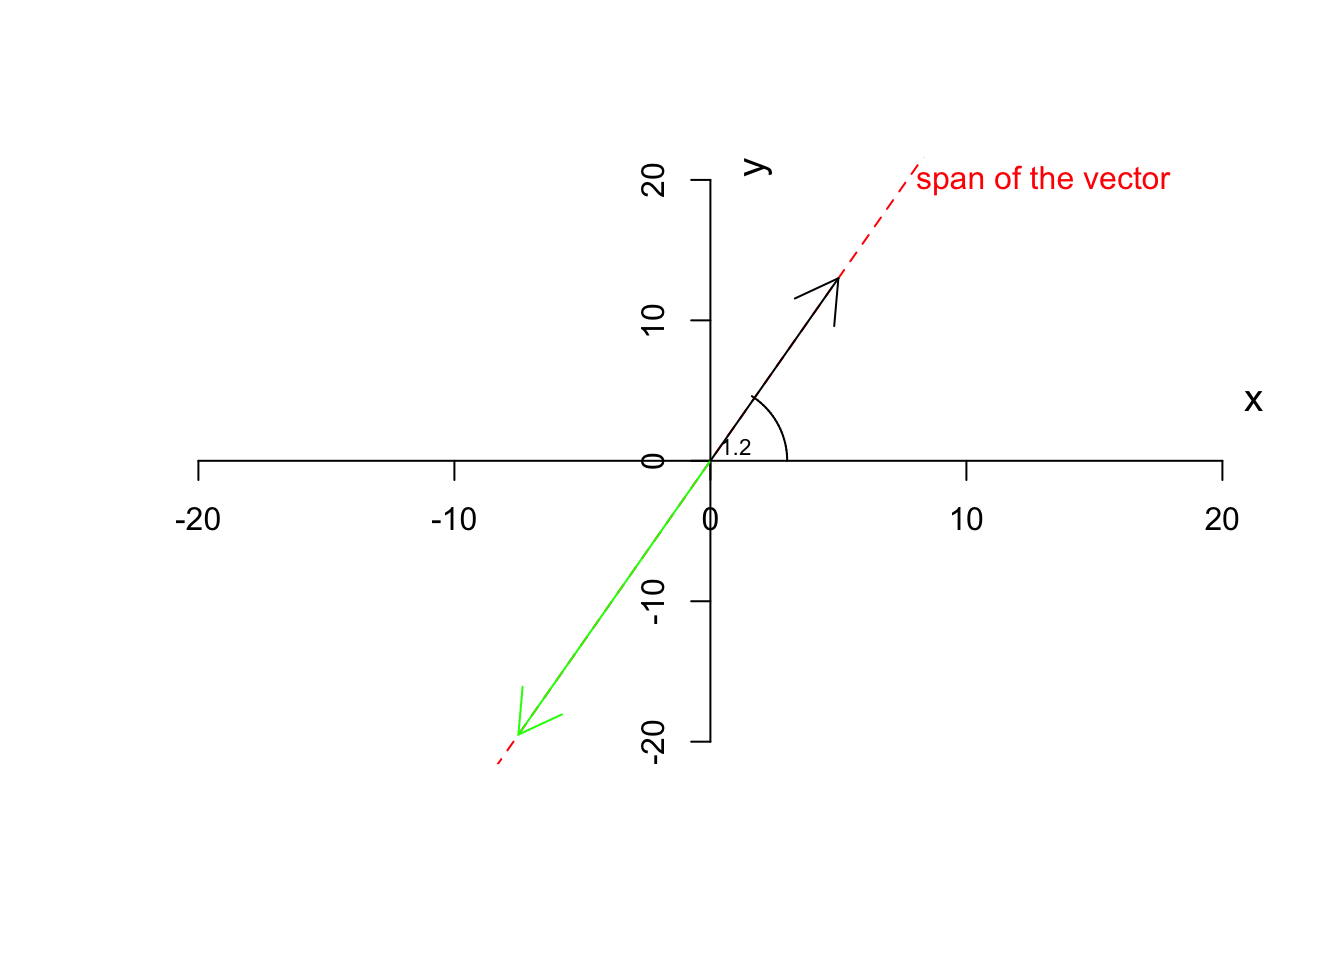
\includegraphics{PCA_files/figure-latex/spaceex8-1} 

}

\caption{Multiplying a vector by a negative scalar}\label{fig:spaceex8}
\end{figure}

You see that the green line now points to the negative direction but still stays on the same span (the red dashed line). Let's move on to the addition. Obviously the same applies if we add a scalar to both element of the vector.

Now let's have a look at when we don't have a scalar but have a vector. Let's start with addition and subtraction

\begin{definition}[Vector addition and subtraction]
\protect\hypertarget{def:vaddition}{}{\label{def:vaddition} \iffalse (Vector addition and subtraction) \fi{} }
We can add or substract two vectors only and only if they have the same number of elements. If we have \(\vec{a}=[x,y]\) and \(\vec{b}=[p,z]\) and the addition and subtraction are defined:

\[\vec{c}=\vec{a}+\vec{b}=[x+p, y+z]\]

and

\[\vec{c}=\vec{a}-\vec{b}=[x-p, y-z]\]

Obviously, we take similar element of the vector and add or subtract them resulting to a new vector.
\end{definition}

Let's have a look at what it means using an example. Suppose we have two vectors, \(\vec{a}=[5,13]\) and \(\vec{b}=[3,4]\) we add them together and the result will be

\[\vec{c}=\vec{a}+\vec{b}=[5+3, 13+4]=[8,17]\]
Similarly for subtraction

\[\vec{c}=\vec{a}+\vec{b}=[5-3, 13-4]=[2,9]\]

Graphically and verbaly we can think about this, start with \(\vec{a}=[5,13]\), from the origin go 5 to the right and 13 up. Great! Stop here. Now let's continue with \(\vec{b}=[3,4]\). Go 3 steps further to the right and then go 4 steps up! This is \(\vec{c}=\vec{a}+\vec{b}\)

Let's look at the graphics:

\begin{Shaded}
\begin{Highlighting}[]
\KeywordTok{par}\NormalTok{(}\DataTypeTok{mfrow=}\KeywordTok{c}\NormalTok{(}\DecValTok{1}\NormalTok{,}\DecValTok{2}\NormalTok{))}
\CommentTok{# plot the data for variable 1}
\KeywordTok{plot}\NormalTok{(}\KeywordTok{c}\NormalTok{(}\OperatorTok{-}\DecValTok{20}\NormalTok{,}\DecValTok{20}\NormalTok{),}\KeywordTok{c}\NormalTok{(}\OperatorTok{-}\DecValTok{20}\NormalTok{,}\DecValTok{20}\NormalTok{),}\DataTypeTok{xlab =} \StringTok{""}\NormalTok{,}\DataTypeTok{ylab =} \StringTok{""}\NormalTok{,}
 \DataTypeTok{axes =}\NormalTok{ F,}\DataTypeTok{type =} \StringTok{"n"}\NormalTok{)}

\CommentTok{# plot the axis}
\KeywordTok{axis}\NormalTok{(}\DecValTok{1}\NormalTok{,}\DataTypeTok{cex=}\DecValTok{4}\NormalTok{,}\DataTypeTok{pos =} \KeywordTok{c}\NormalTok{(}\DecValTok{0}\NormalTok{,}\DecValTok{0}\NormalTok{) )}
\KeywordTok{title}\NormalTok{(}\DataTypeTok{xlab=}\StringTok{"x"}\NormalTok{, }\DataTypeTok{line=}\OperatorTok{-}\DecValTok{10}\NormalTok{, }\DataTypeTok{cex.lab=}\FloatTok{1.2}\NormalTok{,}\DataTypeTok{adj=}\DecValTok{1}\NormalTok{)}
\KeywordTok{axis}\NormalTok{(}\DecValTok{2}\NormalTok{,}\DataTypeTok{cex=}\DecValTok{4}\NormalTok{,}\DataTypeTok{pos =} \KeywordTok{c}\NormalTok{(}\DecValTok{0}\NormalTok{,}\DecValTok{0}\NormalTok{) )}
\KeywordTok{title}\NormalTok{(}\DataTypeTok{ylab=}\StringTok{"y"}\NormalTok{, }\DataTypeTok{line=}\OperatorTok{-}\DecValTok{16}\NormalTok{, }\DataTypeTok{cex.lab=}\FloatTok{1.2}\NormalTok{,}\DataTypeTok{adj=}\DecValTok{1}\NormalTok{)}
\CommentTok{# plot arrow and text}

\KeywordTok{arrows}\NormalTok{(}\DecValTok{0}\NormalTok{,}\DecValTok{0}\NormalTok{,}\DecValTok{5}\NormalTok{,}\DecValTok{13}\NormalTok{,}\DataTypeTok{col=}\StringTok{"green"}\NormalTok{)}

\KeywordTok{arrows}\NormalTok{(}\DecValTok{0}\NormalTok{,}\DecValTok{0}\NormalTok{,}\DecValTok{3}\NormalTok{,}\DecValTok{4}\NormalTok{,}\DataTypeTok{col=}\StringTok{"red"}\NormalTok{)}
\KeywordTok{title}\NormalTok{(}\StringTok{"Original vectors a and b"}\NormalTok{)}


\KeywordTok{plot}\NormalTok{(}\KeywordTok{c}\NormalTok{(}\OperatorTok{-}\DecValTok{20}\NormalTok{,}\DecValTok{20}\NormalTok{),}\KeywordTok{c}\NormalTok{(}\OperatorTok{-}\DecValTok{20}\NormalTok{,}\DecValTok{20}\NormalTok{),}\DataTypeTok{xlab =} \StringTok{""}\NormalTok{,}\DataTypeTok{ylab =} \StringTok{""}\NormalTok{,}
 \DataTypeTok{axes =}\NormalTok{ F,}\DataTypeTok{type =} \StringTok{"n"}\NormalTok{)}



\CommentTok{# plot the axis}
\KeywordTok{axis}\NormalTok{(}\DecValTok{1}\NormalTok{,}\DataTypeTok{cex=}\DecValTok{4}\NormalTok{,}\DataTypeTok{pos =} \KeywordTok{c}\NormalTok{(}\DecValTok{0}\NormalTok{,}\DecValTok{0}\NormalTok{) )}
\KeywordTok{title}\NormalTok{(}\DataTypeTok{xlab=}\StringTok{"x"}\NormalTok{, }\DataTypeTok{line=}\OperatorTok{-}\DecValTok{10}\NormalTok{, }\DataTypeTok{cex.lab=}\FloatTok{1.2}\NormalTok{,}\DataTypeTok{adj=}\DecValTok{1}\NormalTok{)}
\KeywordTok{axis}\NormalTok{(}\DecValTok{2}\NormalTok{,}\DataTypeTok{cex=}\DecValTok{4}\NormalTok{,}\DataTypeTok{pos =} \KeywordTok{c}\NormalTok{(}\DecValTok{0}\NormalTok{,}\DecValTok{0}\NormalTok{) )}
\KeywordTok{title}\NormalTok{(}\DataTypeTok{ylab=}\StringTok{"y"}\NormalTok{, }\DataTypeTok{line=}\OperatorTok{-}\DecValTok{16}\NormalTok{, }\DataTypeTok{cex.lab=}\FloatTok{1.2}\NormalTok{,}\DataTypeTok{adj=}\DecValTok{1}\NormalTok{)}
\CommentTok{# plot arrow and text}
\KeywordTok{arrows}\NormalTok{(}\DecValTok{0}\NormalTok{,}\DecValTok{0}\NormalTok{,}\DecValTok{5}\NormalTok{,}\DecValTok{13}\NormalTok{,}\DataTypeTok{col=}\StringTok{"red"}\NormalTok{)}

\KeywordTok{arrows}\NormalTok{(}\DecValTok{5}\NormalTok{,}\DecValTok{13}\NormalTok{,}\DecValTok{8}\NormalTok{,}\DecValTok{17}\NormalTok{,}\DataTypeTok{col=}\StringTok{"green"}\NormalTok{)}
\KeywordTok{title}\NormalTok{(}\StringTok{"Addtion and a and b"}\NormalTok{)}

\KeywordTok{arrows}\NormalTok{(}\DecValTok{0}\NormalTok{,}\DecValTok{0}\NormalTok{,}\DecValTok{8}\NormalTok{,}\DecValTok{17}\NormalTok{,}\DataTypeTok{col=}\StringTok{"black"}\NormalTok{)}


\CommentTok{# draw circle}
\NormalTok{plotrix}\OperatorTok{::}\KeywordTok{draw.arc}\NormalTok{(}\DecValTok{0}\NormalTok{,}\DecValTok{0}\NormalTok{,}\DecValTok{3}\NormalTok{,}\DataTypeTok{angle2=}\DecValTok{1}\NormalTok{)}

\KeywordTok{text}\NormalTok{(}\DecValTok{1}\NormalTok{,}\DecValTok{1}\NormalTok{,}\StringTok{"1.2"}\NormalTok{,}\DataTypeTok{cex=}\FloatTok{0.7}\NormalTok{)}
\end{Highlighting}
\end{Shaded}

\begin{figure}

{\centering 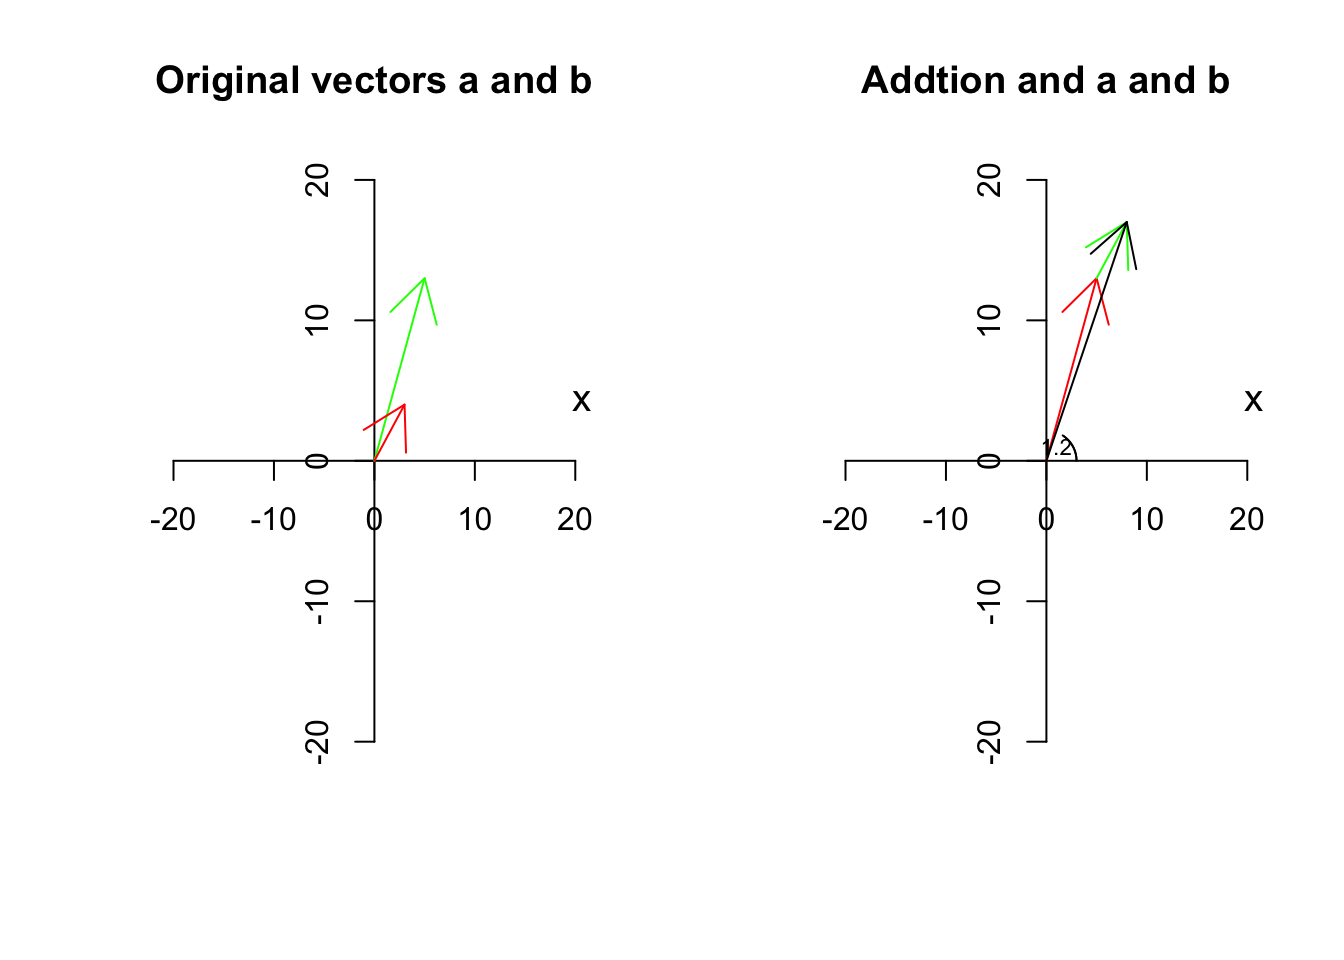
\includegraphics{PCA_files/figure-latex/spaceex9-1} 

}

\caption{Adding two vectors}\label{fig:spaceex9}
\end{figure}

We have two vectors, \(\vec{a}\) is red, \(\vec{b}\) is green and \(\vec{c}\) is black. So the black one is the resulting vecotr. Has it changed span?

Let's look at the graphics:

\begin{Shaded}
\begin{Highlighting}[]
\KeywordTok{par}\NormalTok{(}\DataTypeTok{mfrow=}\KeywordTok{c}\NormalTok{(}\DecValTok{1}\NormalTok{,}\DecValTok{1}\NormalTok{))}
\CommentTok{# plot the data for variable 1}
\KeywordTok{plot}\NormalTok{(}\KeywordTok{c}\NormalTok{(}\OperatorTok{-}\DecValTok{20}\NormalTok{,}\DecValTok{20}\NormalTok{),}\KeywordTok{c}\NormalTok{(}\OperatorTok{-}\DecValTok{20}\NormalTok{,}\DecValTok{20}\NormalTok{),}\DataTypeTok{xlab =} \StringTok{""}\NormalTok{,}\DataTypeTok{ylab =} \StringTok{""}\NormalTok{,}
 \DataTypeTok{axes =}\NormalTok{ F,}\DataTypeTok{type =} \StringTok{"n"}\NormalTok{)}

\CommentTok{# plot the axis}
\KeywordTok{axis}\NormalTok{(}\DecValTok{1}\NormalTok{,}\DataTypeTok{cex=}\DecValTok{4}\NormalTok{,}\DataTypeTok{pos =} \KeywordTok{c}\NormalTok{(}\DecValTok{0}\NormalTok{,}\DecValTok{0}\NormalTok{) )}
\KeywordTok{title}\NormalTok{(}\DataTypeTok{xlab=}\StringTok{"x"}\NormalTok{, }\DataTypeTok{line=}\OperatorTok{-}\DecValTok{10}\NormalTok{, }\DataTypeTok{cex.lab=}\FloatTok{1.2}\NormalTok{,}\DataTypeTok{adj=}\DecValTok{1}\NormalTok{)}
\KeywordTok{axis}\NormalTok{(}\DecValTok{2}\NormalTok{,}\DataTypeTok{cex=}\DecValTok{4}\NormalTok{,}\DataTypeTok{pos =} \KeywordTok{c}\NormalTok{(}\DecValTok{0}\NormalTok{,}\DecValTok{0}\NormalTok{) )}
\KeywordTok{title}\NormalTok{(}\DataTypeTok{ylab=}\StringTok{"y"}\NormalTok{, }\DataTypeTok{line=}\OperatorTok{-}\DecValTok{16}\NormalTok{, }\DataTypeTok{cex.lab=}\FloatTok{1.2}\NormalTok{,}\DataTypeTok{adj=}\DecValTok{1}\NormalTok{)}
\CommentTok{# plot arrow }
\KeywordTok{arrows}\NormalTok{(}\DecValTok{0}\NormalTok{,}\DecValTok{0}\NormalTok{,}\DecValTok{8}\NormalTok{,}\DecValTok{17}\NormalTok{,}\DataTypeTok{col=}\StringTok{"black"}\NormalTok{)}

\CommentTok{# plot span}

 \KeywordTok{segments}\NormalTok{(}\OperatorTok{-}\DecValTok{500}\NormalTok{,}\OperatorTok{-}\DecValTok{1300}\NormalTok{,}\DecValTok{500}\NormalTok{,}\DecValTok{1300}\NormalTok{,}\DataTypeTok{col =} \StringTok{"red"}\NormalTok{,}\DataTypeTok{lty =} \StringTok{"dashed"}\NormalTok{)}
\KeywordTok{text}\NormalTok{(}\DecValTok{13}\NormalTok{,}\DecValTok{20}\NormalTok{,}\StringTok{"span of the vector a"}\NormalTok{,}\DataTypeTok{col=}\StringTok{"red"}\NormalTok{)}


 \KeywordTok{segments}\NormalTok{(}\OperatorTok{-}\DecValTok{300}\NormalTok{,}\OperatorTok{-}\DecValTok{400}\NormalTok{,}\DecValTok{300}\NormalTok{,}\DecValTok{400}\NormalTok{,}\DataTypeTok{col =} \StringTok{"green"}\NormalTok{,}\DataTypeTok{lty =} \StringTok{"dashed"}\NormalTok{)}
\KeywordTok{text}\NormalTok{(}\DecValTok{13}\NormalTok{,}\DecValTok{10}\NormalTok{,}\StringTok{"span of the vector b"}\NormalTok{,}\DataTypeTok{col=}\StringTok{"green"}\NormalTok{)}


\KeywordTok{segments}\NormalTok{(}\OperatorTok{-}\DecValTok{800}\NormalTok{,}\OperatorTok{-}\DecValTok{1700}\NormalTok{,}\DecValTok{800}\NormalTok{,}\DecValTok{1700}\NormalTok{,}\DataTypeTok{col =} \StringTok{"black"}\NormalTok{,}\DataTypeTok{lty =} \StringTok{"dashed"}\NormalTok{)}
\end{Highlighting}
\end{Shaded}

\begin{figure}

{\centering 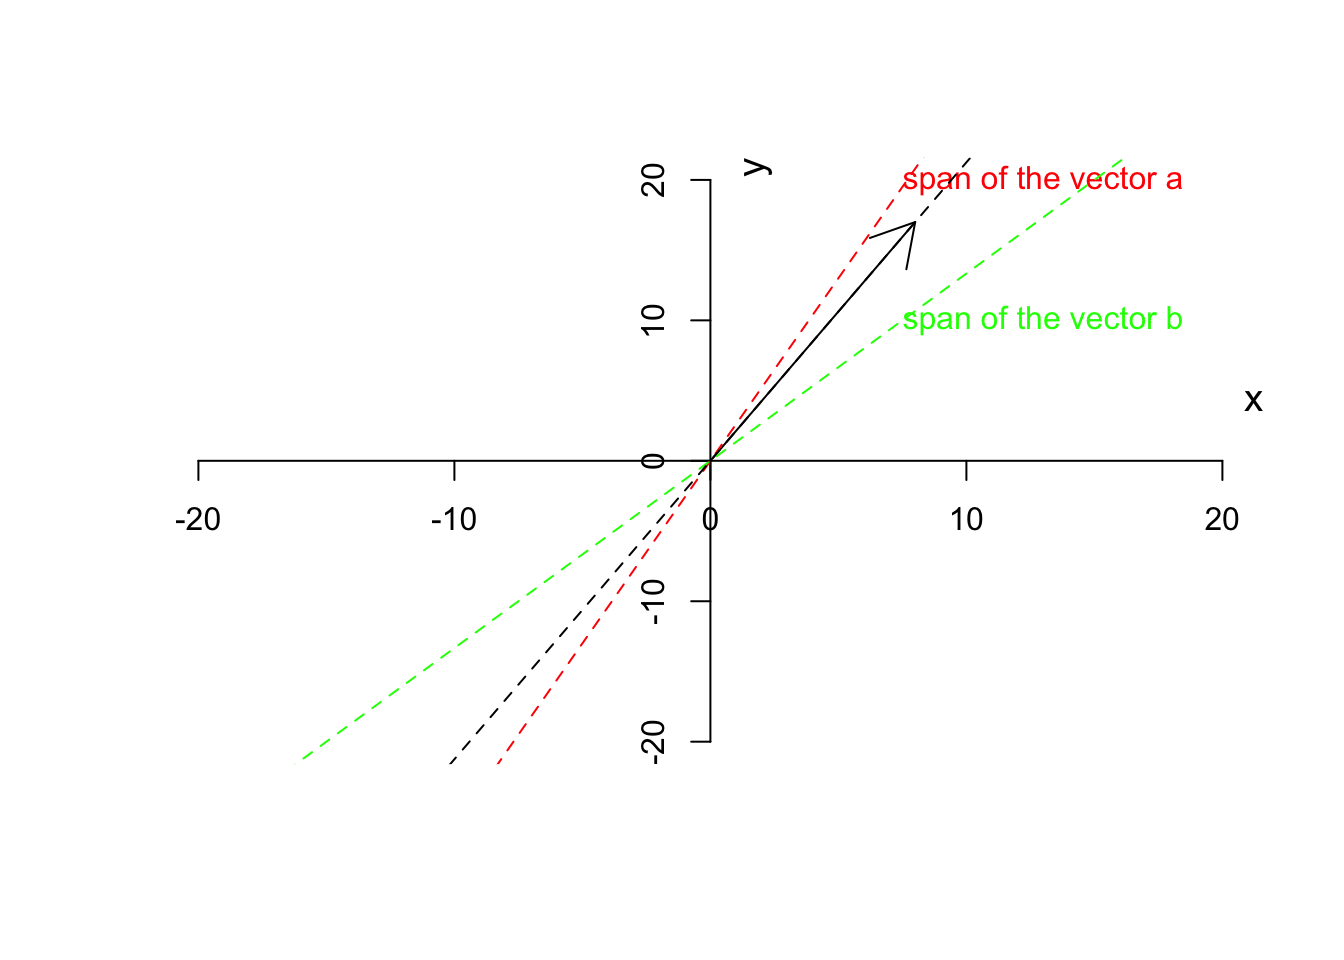
\includegraphics{PCA_files/figure-latex/spaceex10-1} 

}

\caption{Span of vector a, b and c}\label{fig:spaceex10}
\end{figure}

You can obviously see that the span the \(\vec{c}\) (the black dashed line) is not on either of \(\vec{a}\) and \$\vec{b}. We will later talk about why this is important. Perhaps by now you got the point that vectors are not just a list of numbers (like expression a gene for 10 samples) but rather a direction and magnitude.

There are three more things to talk about before moving forward to the next section.

First is that we can normalize a vector to have magnitude of 1 but keep its direction. This can be simply down by diving every element of the vector by its magnitude.

\[\frac{\vec{a}}{\|\vec{a}\|}=[\frac{x}{\|\vec{a}\|},\frac{y}{\|\vec{a}\|}]\]

This will give a normalized or unit vector which the same direction but magnitude of 1. This is handy because we have a vector irrespective of the magnitude but we can multiply it with a scalar to go back to the same vector as we had before.

For example, if we have \(\vec{a}=[3,13]\) we can calculate its magnitude as \(\sqrt{3^2+13^2}=13.3\) giving us the unit vector of \(\hat{a}=[\frac{3}{13.3},\frac{13}{13.3}]=[0.22,0.97]\). This will come handy later when we do a PCA.

\begin{Shaded}
\begin{Highlighting}[]
\KeywordTok{par}\NormalTok{(}\DataTypeTok{mfrow=}\KeywordTok{c}\NormalTok{(}\DecValTok{1}\NormalTok{,}\DecValTok{1}\NormalTok{))}
\CommentTok{# plot the data for variable 1}
\KeywordTok{plot}\NormalTok{(}\KeywordTok{c}\NormalTok{(}\OperatorTok{-}\DecValTok{20}\NormalTok{,}\DecValTok{20}\NormalTok{),}\KeywordTok{c}\NormalTok{(}\OperatorTok{-}\DecValTok{20}\NormalTok{,}\DecValTok{20}\NormalTok{),}\DataTypeTok{xlab =} \StringTok{""}\NormalTok{,}\DataTypeTok{ylab =} \StringTok{""}\NormalTok{,}
 \DataTypeTok{axes =}\NormalTok{ F,}\DataTypeTok{type =} \StringTok{"n"}\NormalTok{)}

\CommentTok{# plot the axis}
\KeywordTok{axis}\NormalTok{(}\DecValTok{1}\NormalTok{,}\DataTypeTok{cex=}\DecValTok{4}\NormalTok{,}\DataTypeTok{pos =} \KeywordTok{c}\NormalTok{(}\DecValTok{0}\NormalTok{,}\DecValTok{0}\NormalTok{) )}
\KeywordTok{title}\NormalTok{(}\DataTypeTok{xlab=}\StringTok{"x"}\NormalTok{, }\DataTypeTok{line=}\OperatorTok{-}\DecValTok{10}\NormalTok{, }\DataTypeTok{cex.lab=}\FloatTok{1.2}\NormalTok{,}\DataTypeTok{adj=}\DecValTok{1}\NormalTok{)}
\KeywordTok{axis}\NormalTok{(}\DecValTok{2}\NormalTok{,}\DataTypeTok{cex=}\DecValTok{4}\NormalTok{,}\DataTypeTok{pos =} \KeywordTok{c}\NormalTok{(}\DecValTok{0}\NormalTok{,}\DecValTok{0}\NormalTok{) )}
\KeywordTok{title}\NormalTok{(}\DataTypeTok{ylab=}\StringTok{"y"}\NormalTok{, }\DataTypeTok{line=}\OperatorTok{-}\DecValTok{16}\NormalTok{, }\DataTypeTok{cex.lab=}\FloatTok{1.2}\NormalTok{,}\DataTypeTok{adj=}\DecValTok{1}\NormalTok{)}
\CommentTok{# plot arrow }
\KeywordTok{arrows}\NormalTok{(}\DecValTok{0}\NormalTok{,}\DecValTok{0}\NormalTok{,}\DecValTok{3}\NormalTok{,}\DecValTok{13}\NormalTok{,}\DataTypeTok{col=}\StringTok{"black"}\NormalTok{)}

\KeywordTok{arrows}\NormalTok{(}\DecValTok{0}\NormalTok{,}\DecValTok{0}\NormalTok{,}\DecValTok{3}\OperatorTok{/}\KeywordTok{sqrt}\NormalTok{(}\KeywordTok{sum}\NormalTok{(}\KeywordTok{c}\NormalTok{(}\DecValTok{3}\NormalTok{,}\DecValTok{13}\NormalTok{)}\OperatorTok{^}\DecValTok{2}\NormalTok{)),}\DecValTok{13}\OperatorTok{/}\KeywordTok{sqrt}\NormalTok{(}\KeywordTok{sum}\NormalTok{(}\KeywordTok{c}\NormalTok{(}\DecValTok{3}\NormalTok{,}\DecValTok{13}\NormalTok{)}\OperatorTok{^}\DecValTok{2}\NormalTok{)),}\DataTypeTok{col=}\StringTok{"red"}\NormalTok{)}
\end{Highlighting}
\end{Shaded}

\begin{figure}

{\centering 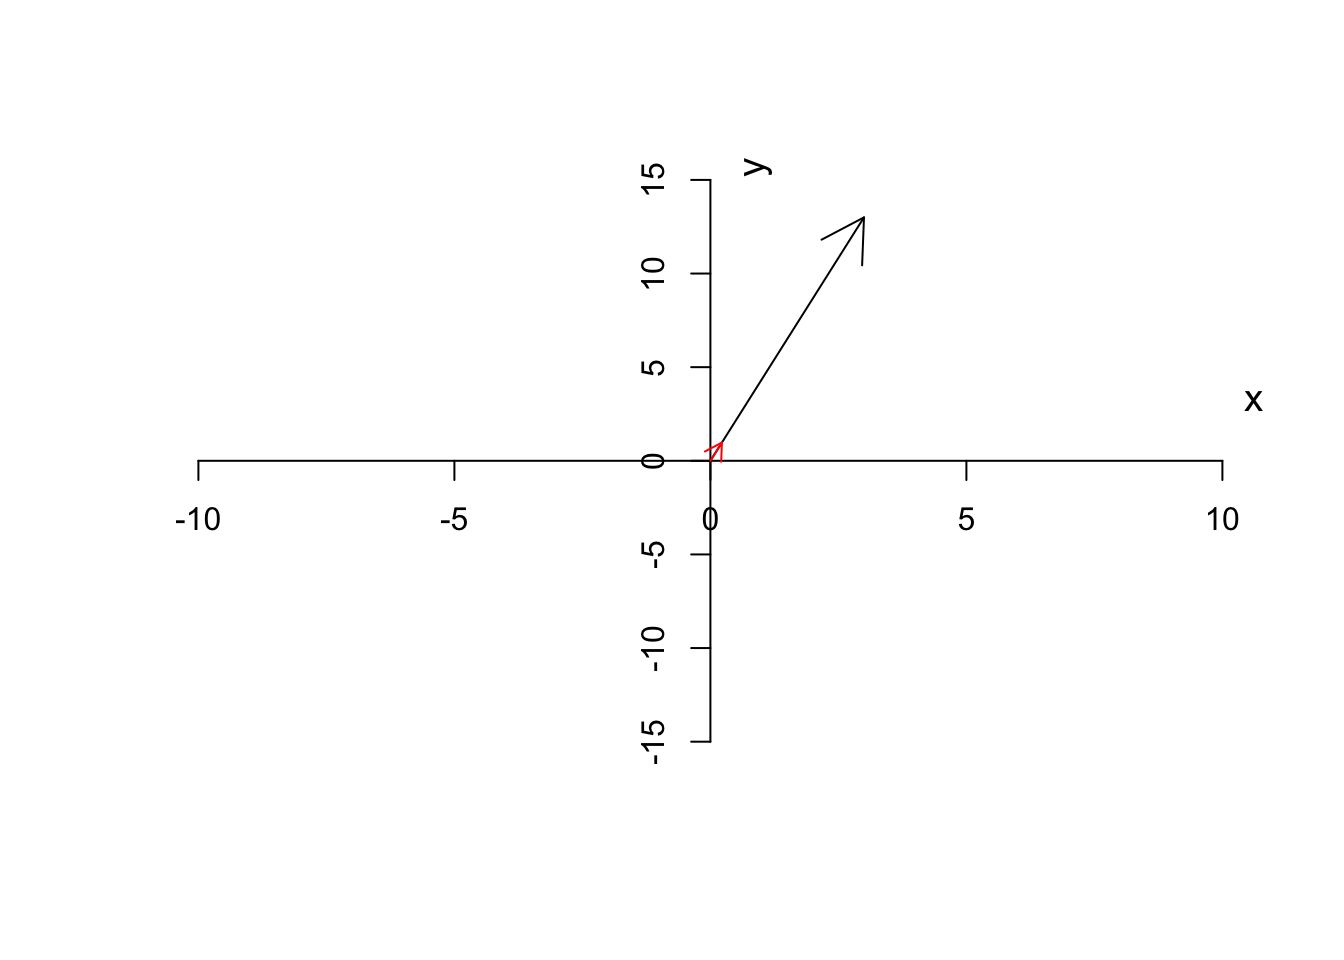
\includegraphics{PCA_files/figure-latex/spaceex11-1} 

}

\caption{Unit vector of a has been depicted}\label{fig:spaceex11}
\end{figure}

As you see in the Figure \ref{fig:spaceex11}, the unit vector (red arrow) has the same direction as the original vector (black arrow) but it's much smaller. In our example, we can multiple the unit vector to \(13.3\) to get back to the original vector as we had.

The second point is that, I guess you noted that we talked about subtraction and addition but we did not talk about multiplication of two vectors. There are two ways of multiply two vectors. One is called cross product that is written as \(\vec{a} \times \vec{b}\) and the second one is called dot product that is written as \(\vec{a}\cdot\vec{b}\). Throughout this chapter, we will only talk about dot product not the cross product. But just to briefly mention it, cross product deals with finding an orthogonal to two other lines. That is if we say \(\vec{a}=\vec{a} \times \vec{b}\), it means that \(\vec{c}\) is a line that is orthogonal to both \(\vec{a}\) and \(\vec{b}\). But Let's ignore it and talk about the dot product.

\begin{definition}[Dot product of two vectors]
\protect\hypertarget{def:dotprod}{}{\label{def:dotprod} \iffalse (Dot product of two vectors) \fi{} }
The dot product of two vectors \(\vec{a}=[x,y]\) and \(\vec{b}=[p,z]\) is define as
\[d=\vec{a}\cdot\vec{b}=x \times p+y \times z\]

It might look a bit fancy, but the concept is that we would like to project or mirror vector \(\vec{a}\) onto the vector \(\vec{b}\) (or perhaps the span of \(\vec{b}\)). We take tip of the vector \(\vec{a}\), draw an orthogonal line from the time to the vector \(\vec{b}\), this gives us the location of vector \(\vec{a}\) on \(\vec{b}\), let's call this new location \(\vec{d}\), we now extend the vector \(\vec{d}\) by the magnitude of \(\|\vec{b}\|\).
\end{definition}

Ok! That was little bit too much. Let's look at an example to make this clear.

Let's draw vector \(\vec{a}\) and \(\vec{b}\)

\begin{Shaded}
\begin{Highlighting}[]
\KeywordTok{par}\NormalTok{(}\DataTypeTok{mfrow=}\KeywordTok{c}\NormalTok{(}\DecValTok{1}\NormalTok{,}\DecValTok{1}\NormalTok{))}
\CommentTok{# plot}
\KeywordTok{plot}\NormalTok{(}\KeywordTok{c}\NormalTok{(}\OperatorTok{-}\DecValTok{5}\NormalTok{,}\DecValTok{40}\NormalTok{),}\KeywordTok{c}\NormalTok{(}\OperatorTok{-}\DecValTok{2}\NormalTok{,}\DecValTok{10}\NormalTok{),}\DataTypeTok{xlab =} \StringTok{""}\NormalTok{,}\DataTypeTok{ylab =} \StringTok{""}\NormalTok{,}
 \DataTypeTok{axes =}\NormalTok{ F,}\DataTypeTok{type =} \StringTok{"n"}\NormalTok{)}


\CommentTok{# plot arrow b}
\KeywordTok{arrows}\NormalTok{(}\DecValTok{0}\NormalTok{,}\DecValTok{0}\NormalTok{,}\DecValTok{20}\NormalTok{,}\DecValTok{0}\NormalTok{,}\DataTypeTok{col=}\StringTok{"blue"}\NormalTok{)}
\CommentTok{# write b}
\KeywordTok{text}\NormalTok{(}\DecValTok{10}\NormalTok{,}\OperatorTok{-}\DecValTok{2}\NormalTok{,}\DataTypeTok{labels =} \StringTok{"b"}\NormalTok{,}\DataTypeTok{col=}\StringTok{"blue"}\NormalTok{)}


\CommentTok{# plot arrow b}
\KeywordTok{arrows}\NormalTok{(}\DecValTok{0}\NormalTok{,}\DataTypeTok{y0 =} \DecValTok{0}\NormalTok{,}\DecValTok{8}\NormalTok{,}\DecValTok{10}\NormalTok{,}\DataTypeTok{col=}\StringTok{"red"}\NormalTok{)}
\CommentTok{# write a}
\KeywordTok{text}\NormalTok{(}\DecValTok{4}\NormalTok{,}\DecValTok{10}\NormalTok{,}\DataTypeTok{labels =} \StringTok{"a"}\NormalTok{,}\DataTypeTok{col=}\StringTok{"red"}\NormalTok{)}

\KeywordTok{segments}\NormalTok{(}\DecValTok{8}\NormalTok{,}\DecValTok{10}\NormalTok{,}\DecValTok{8}\NormalTok{,}\DecValTok{3}\NormalTok{,}\DataTypeTok{lty =} \StringTok{"dashed"}\NormalTok{)}
\end{Highlighting}
\end{Shaded}

\begin{figure}

{\centering 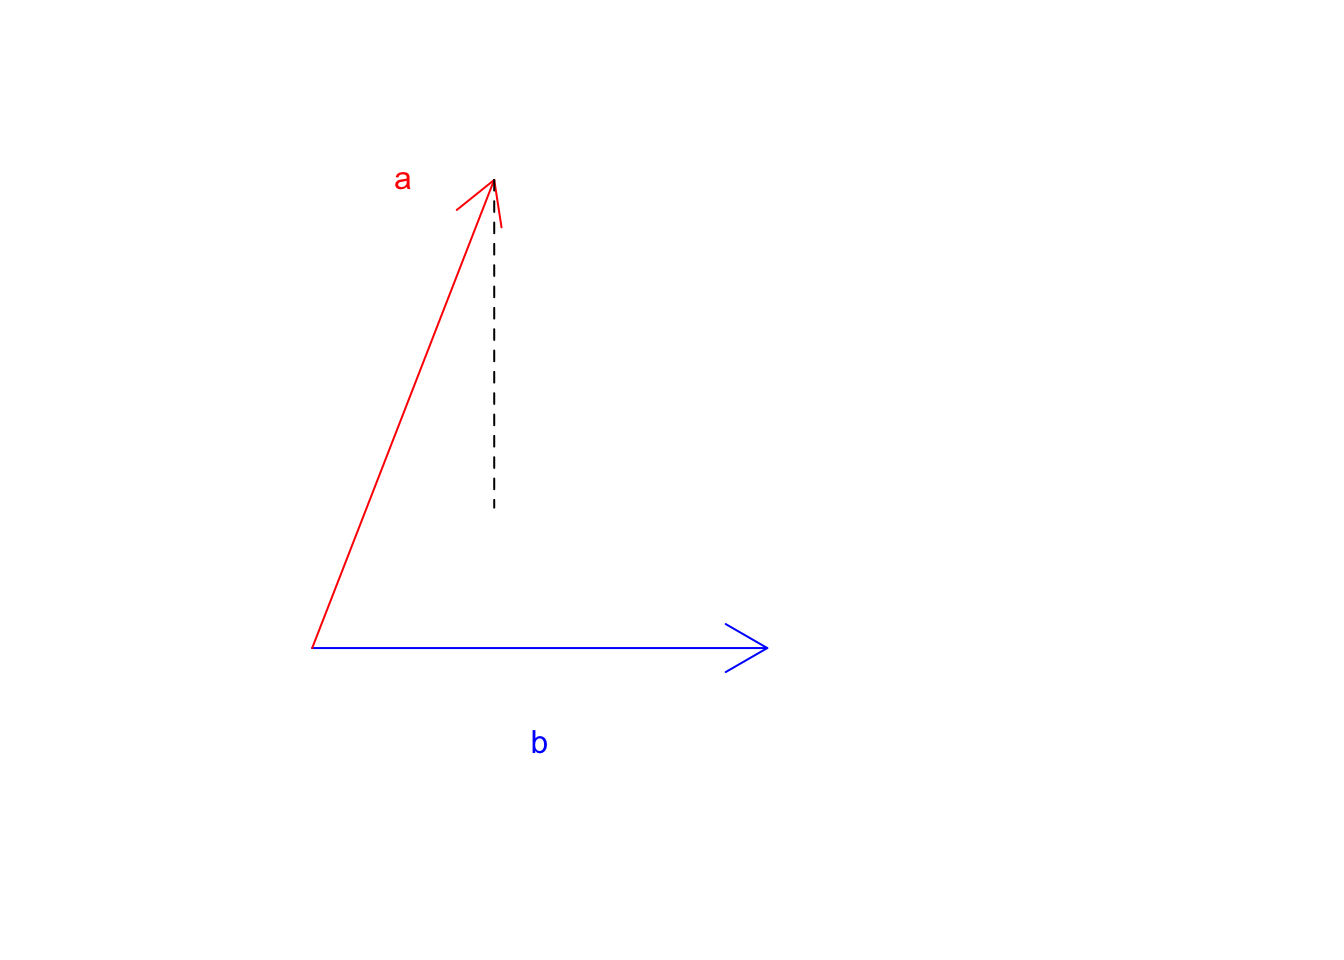
\includegraphics{PCA_files/figure-latex/spaceex12-1} 

}

\caption{Two vectors a and b}\label{fig:spaceex12}
\end{figure}

Great! Where does \(\vec{a}\) land if it starts falling down? Now let's take the tip of the \(\vec{a}\) and draw a line perpendicular to \(\vec{b}\).

\begin{Shaded}
\begin{Highlighting}[]
\KeywordTok{par}\NormalTok{(}\DataTypeTok{mfrow=}\KeywordTok{c}\NormalTok{(}\DecValTok{1}\NormalTok{,}\DecValTok{1}\NormalTok{))}
\CommentTok{# plot}
\KeywordTok{plot}\NormalTok{(}\KeywordTok{c}\NormalTok{(}\OperatorTok{-}\DecValTok{5}\NormalTok{,}\DecValTok{40}\NormalTok{),}\KeywordTok{c}\NormalTok{(}\OperatorTok{-}\DecValTok{2}\NormalTok{,}\DecValTok{10}\NormalTok{),}\DataTypeTok{xlab =} \StringTok{""}\NormalTok{,}\DataTypeTok{ylab =} \StringTok{""}\NormalTok{,}
 \DataTypeTok{axes =}\NormalTok{ F,}\DataTypeTok{type =} \StringTok{"n"}\NormalTok{)}


\CommentTok{# plot arrow b}
\KeywordTok{arrows}\NormalTok{(}\DecValTok{0}\NormalTok{,}\DecValTok{0}\NormalTok{,}\DecValTok{20}\NormalTok{,}\DecValTok{0}\NormalTok{,}\DataTypeTok{col=}\StringTok{"blue"}\NormalTok{)}
\CommentTok{# write b}
\KeywordTok{text}\NormalTok{(}\DecValTok{18}\NormalTok{,}\OperatorTok{-}\DecValTok{1}\NormalTok{,}\DataTypeTok{labels =} \StringTok{"b"}\NormalTok{,}\DataTypeTok{col=}\StringTok{"blue"}\NormalTok{)}


\CommentTok{# plot arrow b}
\KeywordTok{arrows}\NormalTok{(}\DecValTok{0}\NormalTok{,}\DataTypeTok{y0 =} \DecValTok{0}\NormalTok{,}\DecValTok{8}\NormalTok{,}\DecValTok{10}\NormalTok{,}\DataTypeTok{col=}\StringTok{"red"}\NormalTok{)}
\CommentTok{# write a}
\KeywordTok{text}\NormalTok{(}\DecValTok{4}\NormalTok{,}\DecValTok{10}\NormalTok{,}\DataTypeTok{labels =} \StringTok{"a"}\NormalTok{,}\DataTypeTok{col=}\StringTok{"red"}\NormalTok{)}

\KeywordTok{segments}\NormalTok{(}\DecValTok{8}\NormalTok{,}\DecValTok{10}\NormalTok{,}\DecValTok{8}\NormalTok{,}\DecValTok{0}\NormalTok{,}\DataTypeTok{lty =} \StringTok{"dashed"}\NormalTok{)}

\KeywordTok{text}\NormalTok{(}\DecValTok{20}\NormalTok{,}\DecValTok{6}\NormalTok{,}\DataTypeTok{labels =} \StringTok{"perpendicular line (projection line)"}\NormalTok{,}\DataTypeTok{col=}\StringTok{"black"}\NormalTok{)}

\KeywordTok{arrows}\NormalTok{(}\DecValTok{4}\NormalTok{,}\OperatorTok{-}\DecValTok{1}\NormalTok{,}\DecValTok{8}\NormalTok{, }\DecValTok{0}\NormalTok{,}\DataTypeTok{col=}\StringTok{"black"}\NormalTok{)}

\KeywordTok{text}\NormalTok{(}\DecValTok{2}\NormalTok{,}\OperatorTok{-}\FloatTok{1.5}\NormalTok{,}\DataTypeTok{labels =} \StringTok{"projection location"}\NormalTok{,}\DataTypeTok{col=}\StringTok{"black"}\NormalTok{)}
\end{Highlighting}
\end{Shaded}

\begin{figure}

{\centering 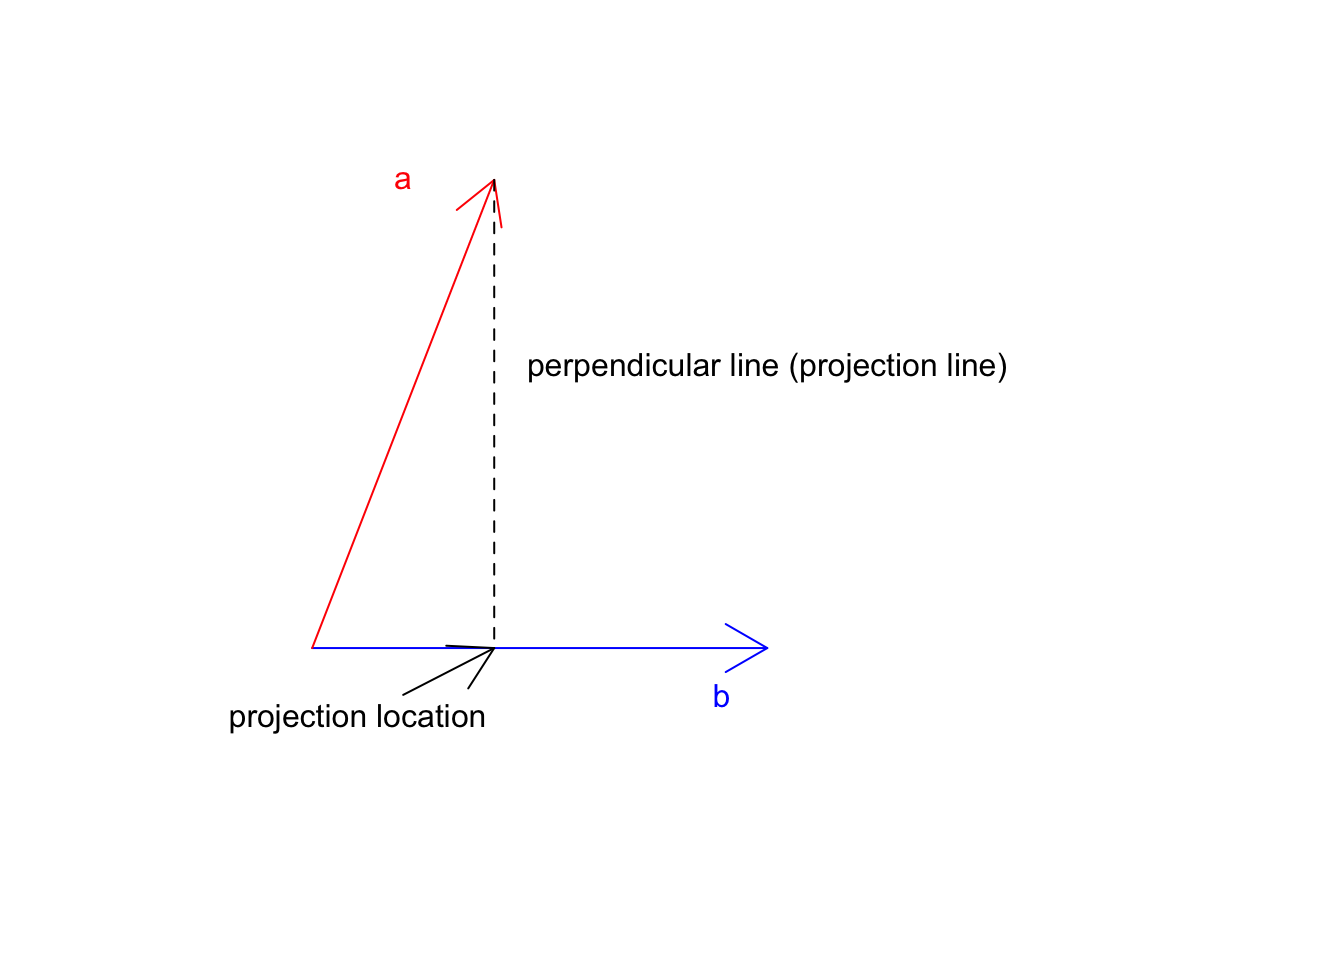
\includegraphics{PCA_files/figure-latex/spaceex13-1} 

}

\caption{Two vectors a and b}\label{fig:spaceex13}
\end{figure}

Now we know the location \(\vec{a}\) on \(\vec{b}\) this is exactly at 8 we can go ahead ahead and multiply this but the magnitude of \(\vec{b}\) (20):

\begin{Shaded}
\begin{Highlighting}[]
\KeywordTok{par}\NormalTok{(}\DataTypeTok{mfrow=}\KeywordTok{c}\NormalTok{(}\DecValTok{1}\NormalTok{,}\DecValTok{1}\NormalTok{))}
\CommentTok{# plot}
\KeywordTok{plot}\NormalTok{(}\KeywordTok{c}\NormalTok{(}\OperatorTok{-}\DecValTok{5}\NormalTok{,}\DecValTok{165}\NormalTok{),}\KeywordTok{c}\NormalTok{(}\OperatorTok{-}\DecValTok{2}\NormalTok{,}\DecValTok{10}\NormalTok{),}\DataTypeTok{xlab =} \StringTok{""}\NormalTok{,}\DataTypeTok{ylab =} \StringTok{""}\NormalTok{,}
 \DataTypeTok{axes =}\NormalTok{ F,}\DataTypeTok{type =} \StringTok{"n"}\NormalTok{)}


\CommentTok{# plot arrow b}
\KeywordTok{arrows}\NormalTok{(}\DecValTok{0}\NormalTok{,}\DecValTok{0}\NormalTok{,}\DecValTok{20}\NormalTok{,}\DecValTok{0}\NormalTok{,}\DataTypeTok{col=}\StringTok{"blue"}\NormalTok{)}
\CommentTok{# write b}
\KeywordTok{text}\NormalTok{(}\DecValTok{18}\NormalTok{,}\OperatorTok{-}\DecValTok{1}\NormalTok{,}\DataTypeTok{labels =} \StringTok{"b"}\NormalTok{,}\DataTypeTok{col=}\StringTok{"blue"}\NormalTok{)}


\CommentTok{# plot arrow b}
\KeywordTok{arrows}\NormalTok{(}\DecValTok{0}\NormalTok{,}\DataTypeTok{y0 =} \DecValTok{0}\NormalTok{,}\DecValTok{8}\NormalTok{,}\DecValTok{10}\NormalTok{,}\DataTypeTok{col=}\StringTok{"red"}\NormalTok{)}
\CommentTok{# write a}
\KeywordTok{text}\NormalTok{(}\DecValTok{4}\NormalTok{,}\DecValTok{10}\NormalTok{,}\DataTypeTok{labels =} \StringTok{"a"}\NormalTok{,}\DataTypeTok{col=}\StringTok{"red"}\NormalTok{)}

\KeywordTok{segments}\NormalTok{(}\DecValTok{8}\NormalTok{,}\DecValTok{10}\NormalTok{,}\DecValTok{8}\NormalTok{,}\DecValTok{0}\NormalTok{,}\DataTypeTok{lty =} \StringTok{"dashed"}\NormalTok{)}

\KeywordTok{text}\NormalTok{(}\DecValTok{50}\NormalTok{,}\DecValTok{6}\NormalTok{,}\DataTypeTok{labels =} \StringTok{"perpendicular line (projection line)"}\NormalTok{,}\DataTypeTok{col=}\StringTok{"black"}\NormalTok{)}

\KeywordTok{arrows}\NormalTok{(}\DecValTok{4}\NormalTok{,}\OperatorTok{-}\DecValTok{1}\NormalTok{,}\DecValTok{8}\NormalTok{, }\DecValTok{0}\NormalTok{,}\DataTypeTok{col=}\StringTok{"black"}\NormalTok{)}

\KeywordTok{text}\NormalTok{(}\DecValTok{10}\NormalTok{,}\OperatorTok{-}\FloatTok{1.5}\NormalTok{,}\DataTypeTok{labels =} \StringTok{"projection location"}\NormalTok{,}\DataTypeTok{col=}\StringTok{"black"}\NormalTok{)}


\KeywordTok{arrows}\NormalTok{(}\DecValTok{0}\NormalTok{,}\DecValTok{0}\NormalTok{,}\DecValTok{8}\OperatorTok{*}\KeywordTok{sqrt}\NormalTok{(}\KeywordTok{sum}\NormalTok{(}\KeywordTok{c}\NormalTok{(}\DecValTok{20}\NormalTok{,}\DecValTok{0}\NormalTok{)}\OperatorTok{^}\DecValTok{2}\NormalTok{)),}\DecValTok{0}\NormalTok{,}\DataTypeTok{col=}\StringTok{"red"}\NormalTok{,}\DataTypeTok{lty =} \StringTok{"dashed"}\NormalTok{)}

\KeywordTok{text}\NormalTok{(}\DecValTok{150}\NormalTok{,}\OperatorTok{-}\DecValTok{2}\NormalTok{,}\DataTypeTok{labels =} \StringTok{"dot product of a.b"}\NormalTok{,}\DataTypeTok{col=}\StringTok{"red"}\NormalTok{)}
\end{Highlighting}
\end{Shaded}

\begin{figure}

{\centering 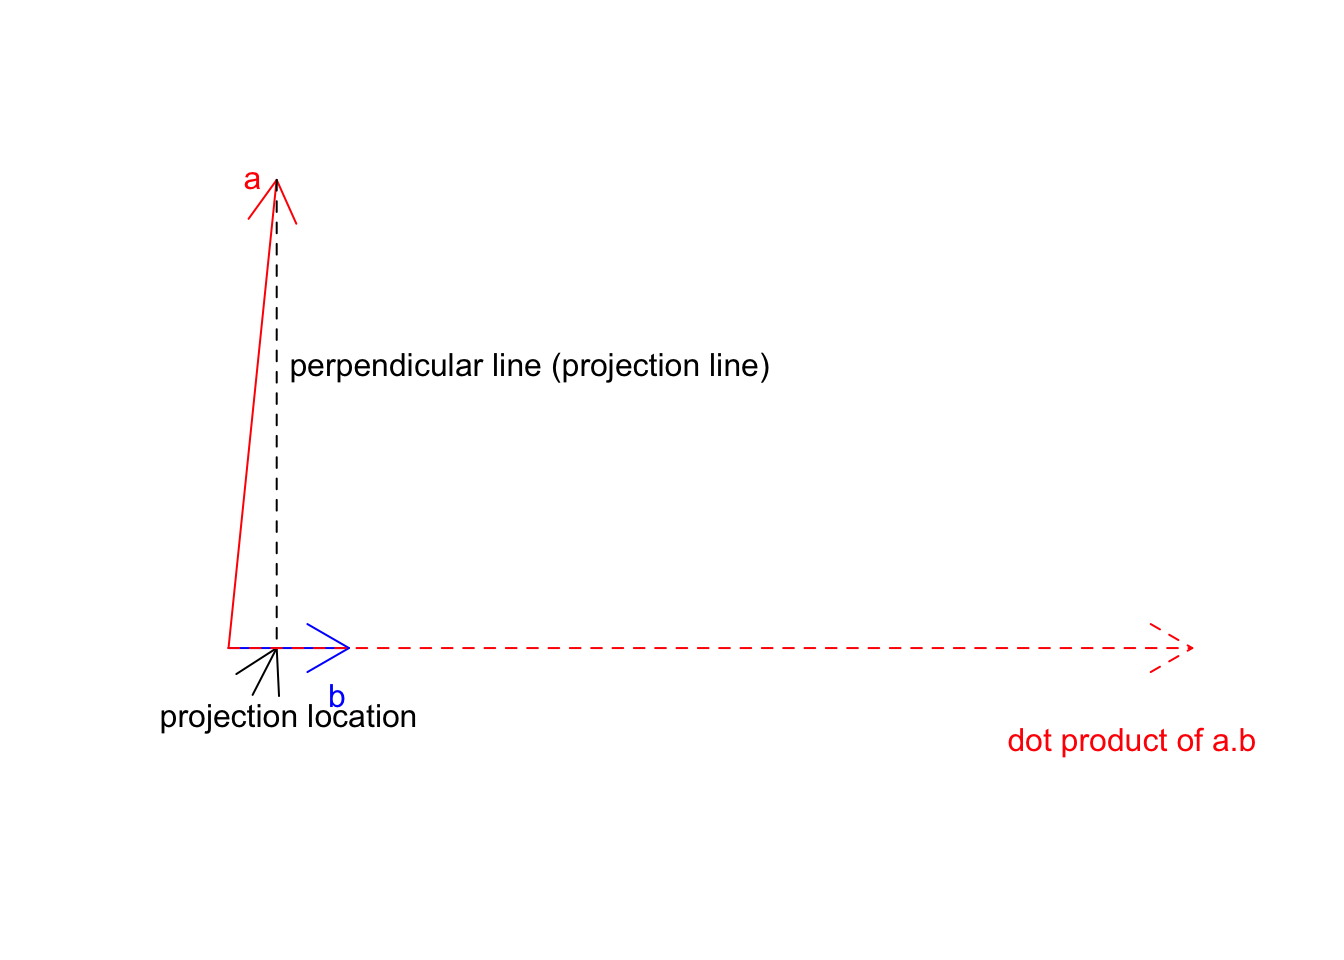
\includegraphics{PCA_files/figure-latex/spaceex14-1} 

}

\caption{Two vectors a and b}\label{fig:spaceex14}
\end{figure}

So the dot product of \(\vec{a}\) on \(\vec{b}\) will be that dashed red line. One way to think about the whole concept is that, we have two different cells with different growth rate. We take cell \emph{a} with some growth apply \emph{b} growth to it. So if \emph{a} is already going 2x, and \emph{b} is going \emph{3} we take 2 and make it 3 times larger! You will see soon that when we work with unit vectors (magnitude of 1), everything becomes much clearer.

The last thing we want to discuss about the vector gets to the definition of space (\ref{def:space}). At that point we did not know much about the vectors. We now can re-define our space as a vector space. The vector space is the set of all possible vectors that we can draw for our dimensions. So far we have been working on two dimensions and we said that we can think about each dimension as a gene or any kind of measurement of interest. Let's consider two genes that can be either silence (zero) or have positive expressions. In reality we barely know the extend of expression of one gene. It might go from zero to some unknown number. But let's assume that it can go all the way to 20. Now we are given all the power in world to be able to induce gene expression to create a human (based on two genes only). Since we know some good deal of linear algebra by now, it's not that difficult! I can go ahead and say i have a person and gene 1=15 and gene 2=5.

\begin{Shaded}
\begin{Highlighting}[]
\KeywordTok{par}\NormalTok{(}\DataTypeTok{mfrow=}\KeywordTok{c}\NormalTok{(}\DecValTok{1}\NormalTok{,}\DecValTok{1}\NormalTok{))}
\CommentTok{# plot}
\KeywordTok{plot}\NormalTok{(}\KeywordTok{c}\NormalTok{(}\DecValTok{0}\NormalTok{,}\DecValTok{20}\NormalTok{),}\KeywordTok{c}\NormalTok{(}\DecValTok{0}\NormalTok{,}\DecValTok{20}\NormalTok{),}\DataTypeTok{xlab =} \StringTok{"Gene 1"}\NormalTok{,}\DataTypeTok{ylab =} \StringTok{"Gene 2"}\NormalTok{,}
 \DataTypeTok{axes =}\NormalTok{ T,}\DataTypeTok{type =} \StringTok{"n"}\NormalTok{)}
\CommentTok{# plot arrow b}
\KeywordTok{arrows}\NormalTok{(}\DecValTok{0}\NormalTok{,}\DecValTok{0}\NormalTok{,}\DecValTok{15}\NormalTok{,}\DecValTok{5}\NormalTok{,}\DataTypeTok{col=}\StringTok{"blue"}\NormalTok{)}
\CommentTok{# add point}
\KeywordTok{points}\NormalTok{(}\DecValTok{15}\NormalTok{,}\DecValTok{5}\NormalTok{,}\DataTypeTok{pch=}\StringTok{"👶"}\NormalTok{)}
\end{Highlighting}
\end{Shaded}

\begin{figure}

{\centering 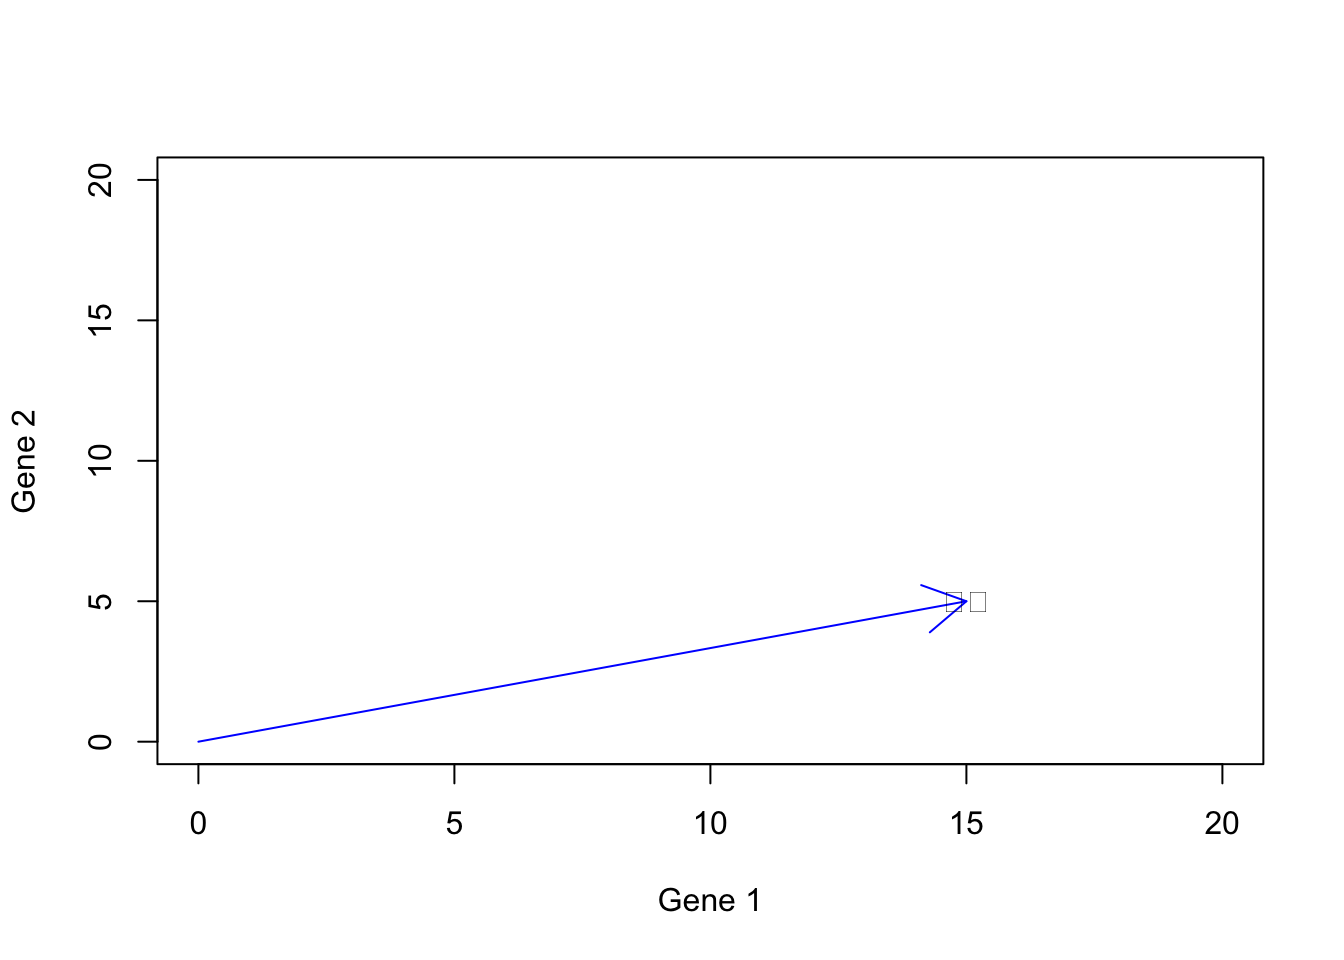
\includegraphics{PCA_files/figure-latex/spaceex15-1} 

}

\caption{Gene expression example}\label{fig:spaceex15}
\end{figure}

If we think a bit, we see that we can create so many humans by these two genes.

\begin{Shaded}
\begin{Highlighting}[]
\KeywordTok{par}\NormalTok{(}\DataTypeTok{mfrow=}\KeywordTok{c}\NormalTok{(}\DecValTok{1}\NormalTok{,}\DecValTok{1}\NormalTok{))}
\CommentTok{# plot}
\KeywordTok{plot}\NormalTok{(}\KeywordTok{c}\NormalTok{(}\DecValTok{0}\NormalTok{,}\DecValTok{20}\NormalTok{),}\KeywordTok{c}\NormalTok{(}\DecValTok{0}\NormalTok{,}\DecValTok{20}\NormalTok{),}\DataTypeTok{xlab =} \StringTok{"Gene 1"}\NormalTok{,}\DataTypeTok{ylab =} \StringTok{"Gene 2"}\NormalTok{,}
 \DataTypeTok{axes =}\NormalTok{ T,}\DataTypeTok{type =} \StringTok{"n"}\NormalTok{)}

\ControlFlowTok{for}\NormalTok{(i }\ControlFlowTok{in} \DecValTok{1}\OperatorTok{:}\DecValTok{100}\NormalTok{)}
\NormalTok{\{}
  \KeywordTok{set.seed}\NormalTok{(i)}
\NormalTok{  g1<-}\KeywordTok{sample}\NormalTok{(}\DecValTok{1}\OperatorTok{:}\DecValTok{20}\NormalTok{,}\DecValTok{1}\NormalTok{)}
   \KeywordTok{set.seed}\NormalTok{(i}\OperatorTok{*}\DecValTok{100}\NormalTok{)}
\NormalTok{  g2<-}\KeywordTok{sample}\NormalTok{(}\DecValTok{1}\OperatorTok{:}\DecValTok{20}\NormalTok{,}\DecValTok{1}\NormalTok{)}
  \CommentTok{# plot arrow b}
\KeywordTok{arrows}\NormalTok{(}\DecValTok{0}\NormalTok{,}\DecValTok{0}\NormalTok{,g1,g2,}\DataTypeTok{col=}\StringTok{"blue"}\NormalTok{)}
\CommentTok{# add point}
\KeywordTok{points}\NormalTok{(g1,g2,}\DataTypeTok{pch=}\StringTok{"👶"}\NormalTok{)}
\NormalTok{\}}
\end{Highlighting}
\end{Shaded}

\begin{figure}

{\centering 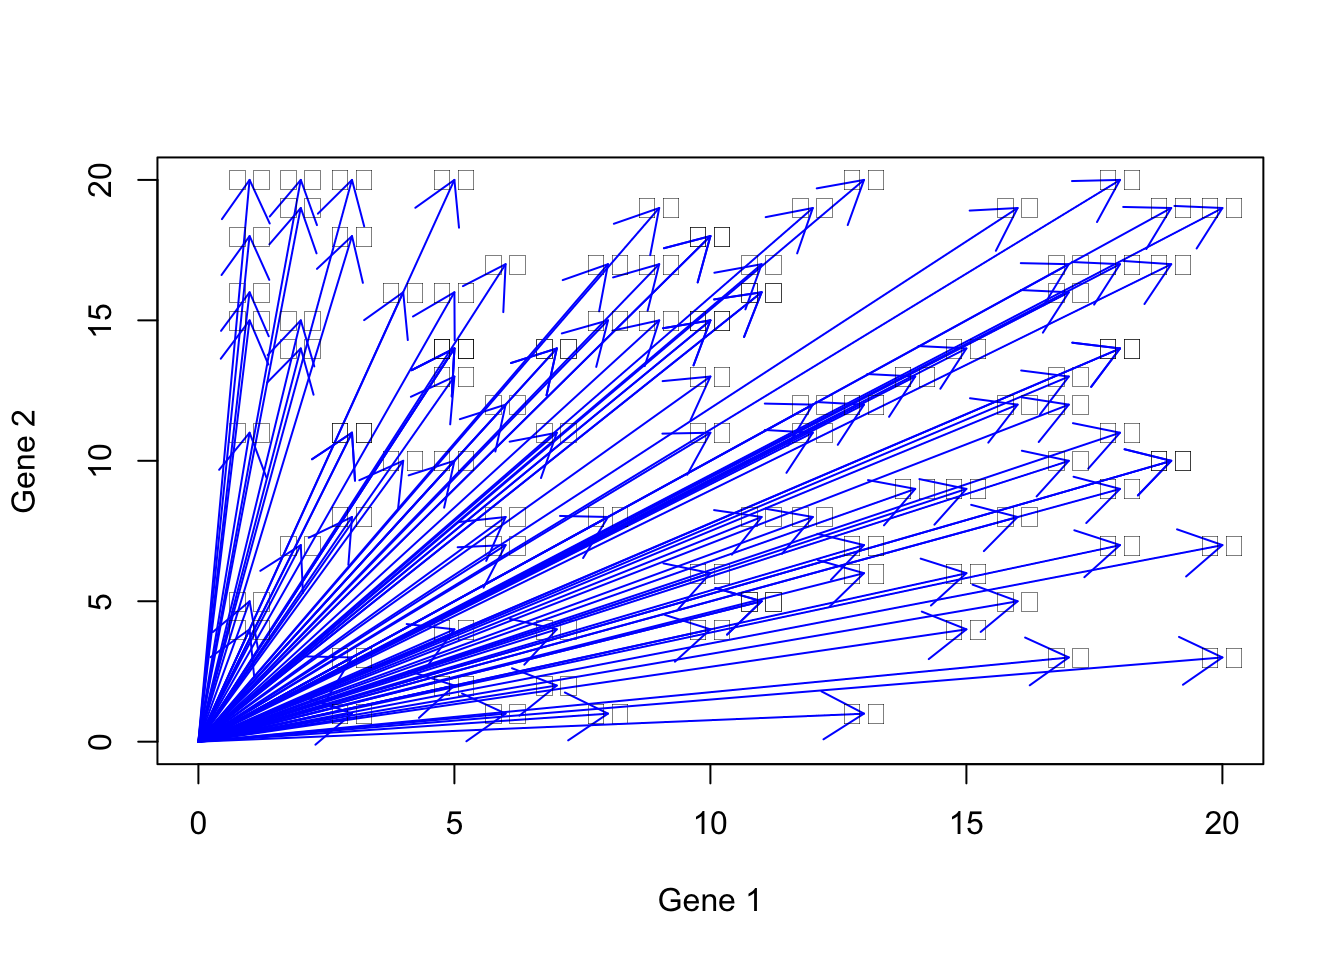
\includegraphics{PCA_files/figure-latex/spaceex16-1} 

}

\caption{Gene expression example with more vectors}\label{fig:spaceex16}
\end{figure}

These possible values, are in fact part of your vector spaces. Essentially all the vectors that can be created are located in this space. The power we were given to work with such space and create what we want were already covered. Our tools are vector addition, subtraction, scalar multiplication and possible dot product. There is only one thing left. We need two buffers, each container the two genes that we can activate/deactivate (\textbf{ONE at the time}), induce the expression, mix the buffers and create a human! Our First buffer we call \emph{b1} is contains both gene 1 and 2, but gene 2 is deactivated, giving us \(b1=[gene1,gene2]\). Let's say we want to represent activated gene by 1 and deactivated gene by zero so b1 one becomes \(b1=[1,0]\). Let's do the same thing for our second buffer, \(b2=[gene1,gene2]\) and turn gene1 to off, \(b1=[0,1]\). Let's again say that we want to create a human (\(h\)) with gene1=15 and gene2=5 so our sample should \(h=[15,5]\). With the tools that we are given and two buffers \(b1=[1,0]\) and \(b2=[0,1]\) how can we reach to \(h=[15,5]\)?

Well, that is not that difficult.

Let's induce gene 1 and call it \(b1i\): \(b1i=15 \times b1=[15 \times 1, 15 \times 0]=[15,0]\). Perfect. We induced the first gene but scalar multiplication.
Now we do this for the second gene and call it \(b2i\): \(b2i=5 \times b2=[5 \times 0, 5 \times 1]=[0,5]\). We now have gene 2 again with scalar multiplication.
How can we mix these two genes and make our first human: \(h=b1i+b2i=[15+0,5+0]=[15,5]\). Yess! We made it!

These small raw vectors (\(\vec{b1}\) and \(vec{b2}\)) together with our operations (addition, multiplication etc) help us to create any possible vector in our space. These are basis vectors.

\begin{definition}[Basis vectors]
\protect\hypertarget{def:bvectors}{}{\label{def:bvectors} \iffalse (Basis vectors) \fi{} }
The basis vectors are a set of vectors that when used in weighted combinition can create any vector in our space. In fact our space itself is defined by the basis vectors. To be called basis vector, these should be pointing to different directions. To be more concrete, the basis vectors should be linearly independent, meaning that they cannot be created by combination of other vectors.

Our ``default'' basis vectors are x={[}1,0{]} and y={[}0,1{]}. That is the only reason that when we plot any data in for examle R, the values of our measurements will be plotted exactly as they are. If we assume anything else than x={[}1,0{]} and y={[}0,1{]}, our plot will end up being something else. So in short, the default basis vector, let us moving around our space to any point and also show us the original angle of our data. We will see later that we can change these basis vectors in order ot rotate our data and see another angle of them. So far let's agree that our basis are {[}0,1{]} and {[}1,0{]} and they are used to construct our data vectors. We can think about this, We with the help of our data change direction, and magnitude of the basis vectors in order to represent our data in the space defined by the basis vectors.
\end{definition}

Let's have a look at the previous example. We start with two basis vectors \(\vec{b1}=[1,0]\) (blue arrow) and \(\vec{b2}=[0,1] (green arrow)\). Our aim was to reach the vector \(\vec{h}=[15,5]\) (black point):

\begin{Shaded}
\begin{Highlighting}[]
\KeywordTok{par}\NormalTok{(}\DataTypeTok{mfrow=}\KeywordTok{c}\NormalTok{(}\DecValTok{1}\NormalTok{,}\DecValTok{1}\NormalTok{))}
\CommentTok{# plot}
\KeywordTok{plot}\NormalTok{(}\KeywordTok{c}\NormalTok{(}\OperatorTok{-}\DecValTok{1}\NormalTok{,}\DecValTok{15}\NormalTok{),}\KeywordTok{c}\NormalTok{(}\OperatorTok{-}\DecValTok{1}\NormalTok{,}\DecValTok{10}\NormalTok{),}\DataTypeTok{xlab =} \StringTok{"Gene 1"}\NormalTok{,}\DataTypeTok{ylab =} \StringTok{"Gene 2"}\NormalTok{,}
 \DataTypeTok{axes =}\NormalTok{ T,}\DataTypeTok{type =} \StringTok{"n"}\NormalTok{)}

\KeywordTok{arrows}\NormalTok{(}\DecValTok{0}\NormalTok{,}\DecValTok{0}\NormalTok{,}\DecValTok{1}\NormalTok{,}\DecValTok{0}\NormalTok{,}\DataTypeTok{col=}\StringTok{"blue"}\NormalTok{,}\DataTypeTok{length =} \FloatTok{0.1}\NormalTok{)}
\KeywordTok{text}\NormalTok{(}\FloatTok{0.5}\NormalTok{,}\OperatorTok{-}\FloatTok{0.5}\NormalTok{,}\StringTok{"b1"}\NormalTok{,}\DataTypeTok{col=}\StringTok{"blue"}\NormalTok{)}

\KeywordTok{arrows}\NormalTok{(}\DecValTok{0}\NormalTok{,}\DecValTok{0}\NormalTok{,}\DecValTok{0}\NormalTok{,}\DecValTok{1}\NormalTok{,}\DataTypeTok{col=}\StringTok{"red"}\NormalTok{,}\DataTypeTok{length =} \FloatTok{0.1}\NormalTok{)}
\KeywordTok{text}\NormalTok{(}\OperatorTok{-}\FloatTok{0.5}\NormalTok{,}\FloatTok{0.5}\NormalTok{,}\StringTok{"b2"}\NormalTok{,}\DataTypeTok{col=}\StringTok{"red"}\NormalTok{)}


\KeywordTok{points}\NormalTok{(}\DecValTok{15}\NormalTok{,}\DecValTok{5}\NormalTok{)}
\end{Highlighting}
\end{Shaded}

\begin{figure}

{\centering 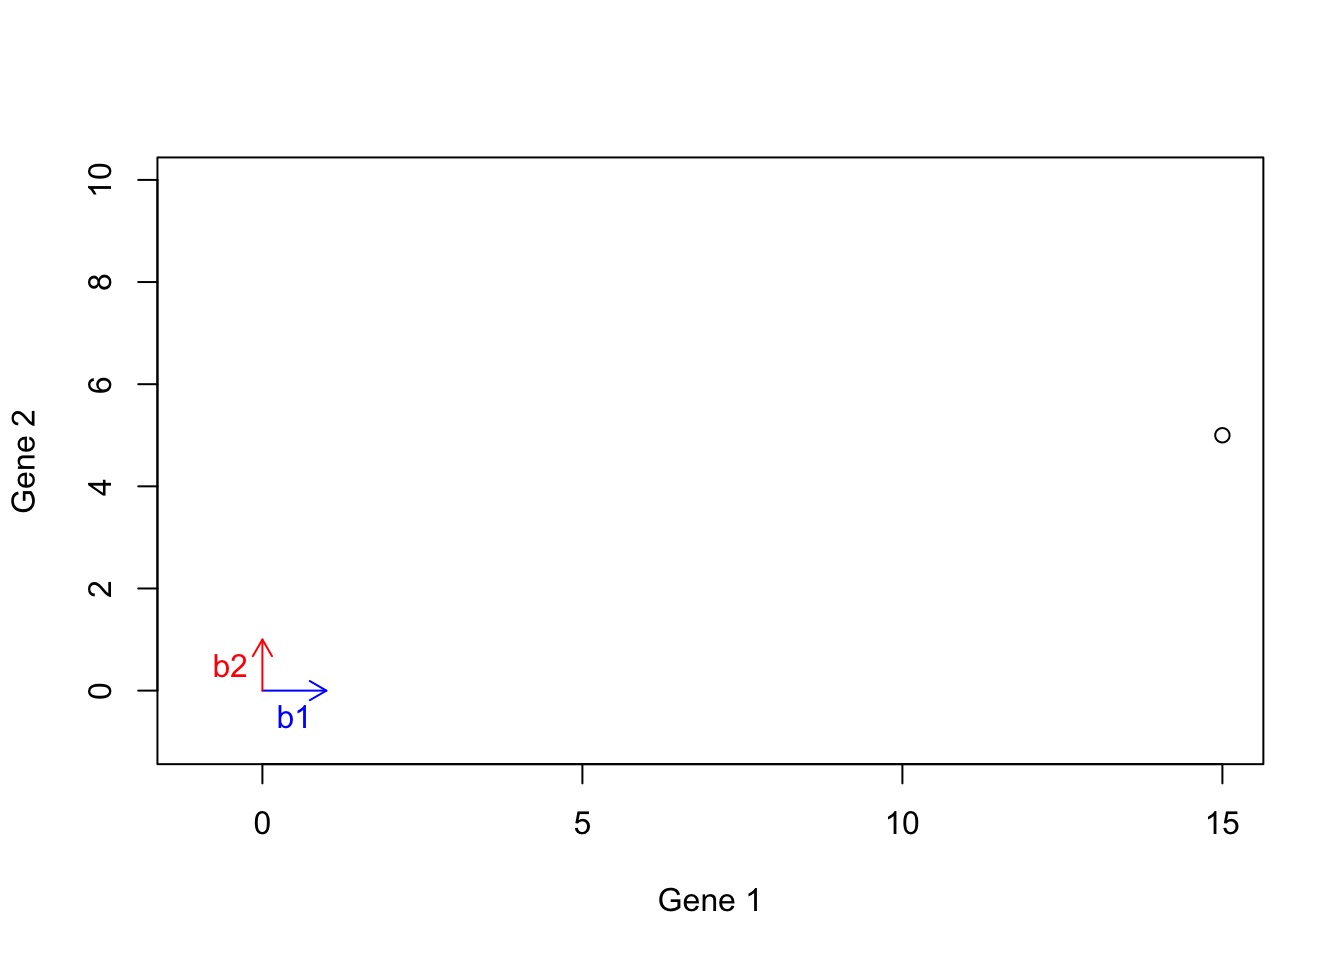
\includegraphics{PCA_files/figure-latex/spaceex17-1} 

}

\caption{Example of basis vectors}\label{fig:spaceex17}
\end{figure}

We first calculate this: \(b1i\): \(b1i=15 \times b1=[15 \times 1, 15 \times 0]=[15,0]\), giving us the dashed arrow:

\begin{Shaded}
\begin{Highlighting}[]
\KeywordTok{par}\NormalTok{(}\DataTypeTok{mfrow=}\KeywordTok{c}\NormalTok{(}\DecValTok{1}\NormalTok{,}\DecValTok{1}\NormalTok{))}
\CommentTok{# plot}
\KeywordTok{plot}\NormalTok{(}\KeywordTok{c}\NormalTok{(}\OperatorTok{-}\DecValTok{1}\NormalTok{,}\DecValTok{15}\NormalTok{),}\KeywordTok{c}\NormalTok{(}\OperatorTok{-}\DecValTok{1}\NormalTok{,}\DecValTok{10}\NormalTok{),}\DataTypeTok{xlab =} \StringTok{"Gene 1"}\NormalTok{,}\DataTypeTok{ylab =} \StringTok{"Gene 2"}\NormalTok{,}
 \DataTypeTok{axes =}\NormalTok{ T,}\DataTypeTok{type =} \StringTok{"n"}\NormalTok{)}

\KeywordTok{arrows}\NormalTok{(}\DecValTok{0}\NormalTok{,}\DecValTok{0}\NormalTok{,}\DecValTok{15}\NormalTok{,}\DecValTok{0}\NormalTok{,}\DataTypeTok{col=}\StringTok{"blue"}\NormalTok{,}\DataTypeTok{length =} \FloatTok{0.1}\NormalTok{,}\DataTypeTok{lty =} \StringTok{"dashed"}\NormalTok{)}
\KeywordTok{text}\NormalTok{(}\DecValTok{7}\NormalTok{,}\OperatorTok{-}\FloatTok{0.5}\NormalTok{,}\StringTok{"b1i"}\NormalTok{,}\DataTypeTok{col=}\StringTok{"blue"}\NormalTok{)}

\KeywordTok{arrows}\NormalTok{(}\DecValTok{0}\NormalTok{,}\DecValTok{0}\NormalTok{,}\DecValTok{0}\NormalTok{,}\DecValTok{1}\NormalTok{,}\DataTypeTok{col=}\StringTok{"red"}\NormalTok{,}\DataTypeTok{length =} \FloatTok{0.1}\NormalTok{)}
\KeywordTok{text}\NormalTok{(}\OperatorTok{-}\FloatTok{0.5}\NormalTok{,}\FloatTok{0.5}\NormalTok{,}\StringTok{"y"}\NormalTok{,}\DataTypeTok{col=}\StringTok{"red"}\NormalTok{)}

\KeywordTok{points}\NormalTok{(}\DecValTok{15}\NormalTok{,}\DecValTok{5}\NormalTok{)}
\end{Highlighting}
\end{Shaded}

\begin{figure}

{\centering 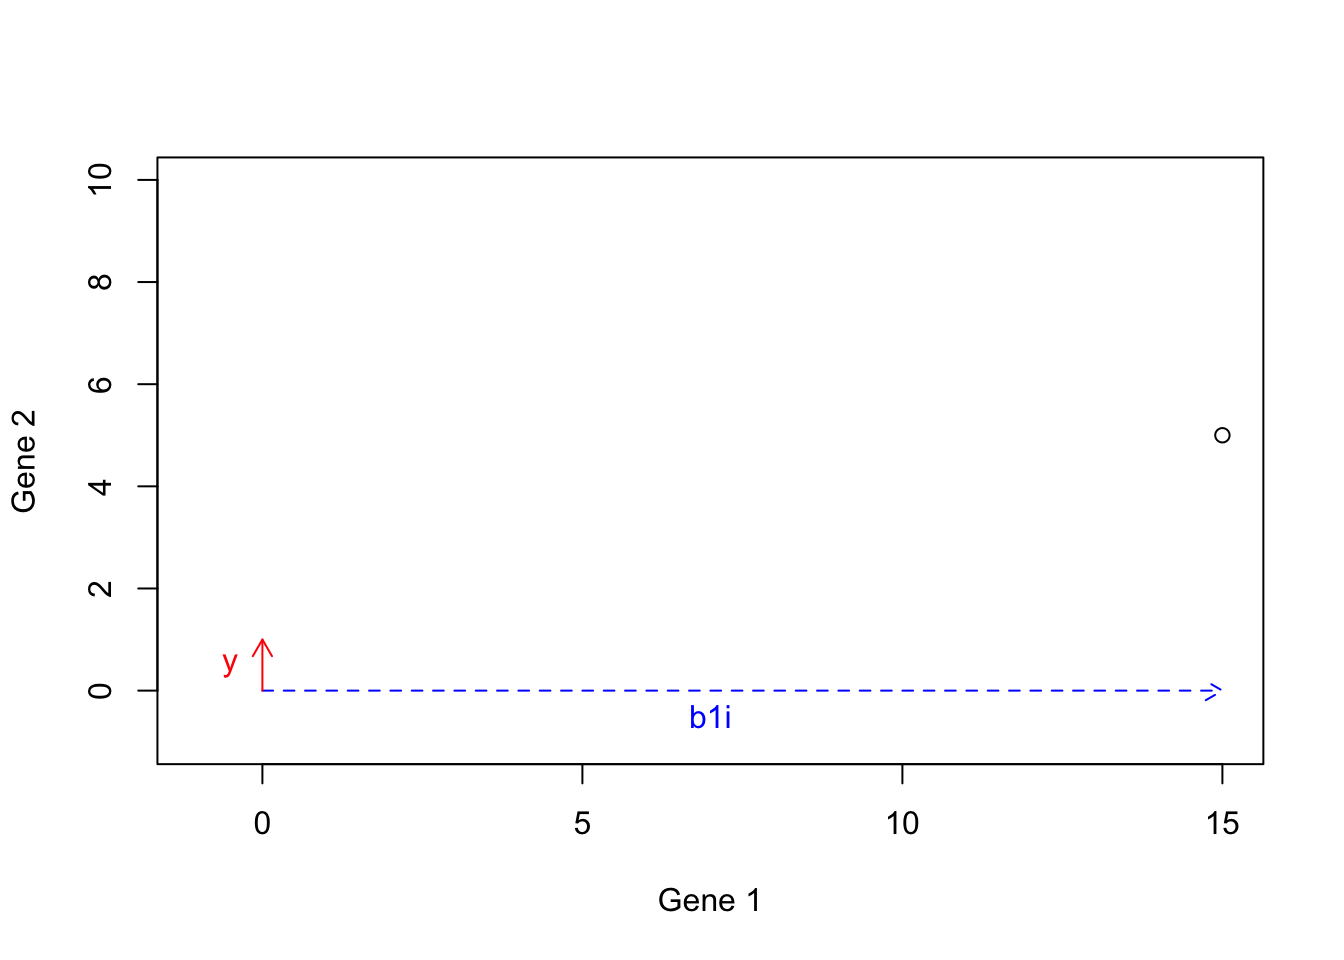
\includegraphics{PCA_files/figure-latex/spaceex18-1} 

}

\caption{Example of basis vectors (scale b1)}\label{fig:spaceex18}
\end{figure}

We then calculate \(b2i\): \(b2i=5 \times b2=[5 \times 0, 5 \times 1]=[0,5]\):

\begin{Shaded}
\begin{Highlighting}[]
\KeywordTok{par}\NormalTok{(}\DataTypeTok{mfrow=}\KeywordTok{c}\NormalTok{(}\DecValTok{1}\NormalTok{,}\DecValTok{1}\NormalTok{))}
\CommentTok{# plot}
\KeywordTok{plot}\NormalTok{(}\KeywordTok{c}\NormalTok{(}\OperatorTok{-}\DecValTok{1}\NormalTok{,}\DecValTok{15}\NormalTok{),}\KeywordTok{c}\NormalTok{(}\OperatorTok{-}\DecValTok{1}\NormalTok{,}\DecValTok{10}\NormalTok{),}\DataTypeTok{xlab =} \StringTok{"Gene 1"}\NormalTok{,}\DataTypeTok{ylab =} \StringTok{"Gene 2"}\NormalTok{,}
 \DataTypeTok{axes =}\NormalTok{ T,}\DataTypeTok{type =} \StringTok{"n"}\NormalTok{)}

\KeywordTok{arrows}\NormalTok{(}\DecValTok{0}\NormalTok{,}\DecValTok{0}\NormalTok{,}\DecValTok{15}\NormalTok{,}\DecValTok{0}\NormalTok{,}\DataTypeTok{col=}\StringTok{"blue"}\NormalTok{,}\DataTypeTok{length =} \FloatTok{0.1}\NormalTok{,}\DataTypeTok{lty =} \StringTok{"dashed"}\NormalTok{)}
\KeywordTok{text}\NormalTok{(}\DecValTok{7}\NormalTok{,}\OperatorTok{-}\FloatTok{0.5}\NormalTok{,}\StringTok{"b1i"}\NormalTok{,}\DataTypeTok{col=}\StringTok{"blue"}\NormalTok{)}

\KeywordTok{arrows}\NormalTok{(}\DecValTok{0}\NormalTok{,}\DecValTok{0}\NormalTok{,}\DecValTok{0}\NormalTok{,}\DecValTok{5}\NormalTok{,}\DataTypeTok{col=}\StringTok{"red"}\NormalTok{,}\DataTypeTok{length =} \FloatTok{0.1}\NormalTok{,}\DataTypeTok{lty =} \StringTok{"dashed"}\NormalTok{)}
\KeywordTok{text}\NormalTok{(}\OperatorTok{-}\FloatTok{0.5}\NormalTok{,}\FloatTok{2.5}\NormalTok{,}\StringTok{"b2i"}\NormalTok{,}\DataTypeTok{col=}\StringTok{"red"}\NormalTok{)}

\KeywordTok{points}\NormalTok{(}\DecValTok{15}\NormalTok{,}\DecValTok{5}\NormalTok{)}
\end{Highlighting}
\end{Shaded}

\begin{figure}

{\centering 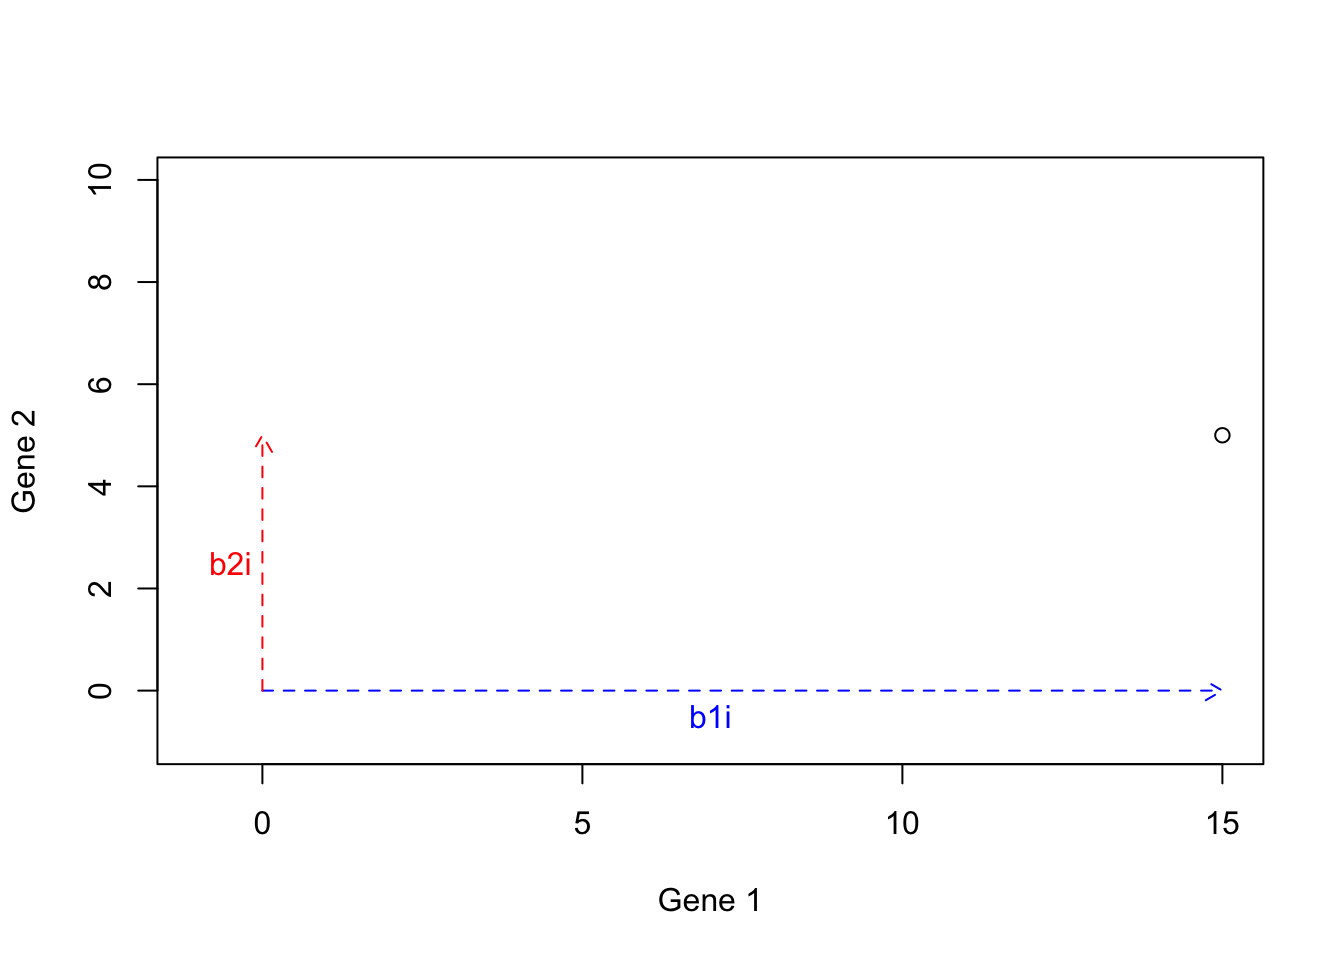
\includegraphics{PCA_files/figure-latex/spaceex19-1} 

}

\caption{Example of basis vectors (scale b2)}\label{fig:spaceex19}
\end{figure}

We can now calculate \(h=b1i+b2i=[15+0,5+0]=[15,5]\):

\begin{Shaded}
\begin{Highlighting}[]
\KeywordTok{par}\NormalTok{(}\DataTypeTok{mfrow=}\KeywordTok{c}\NormalTok{(}\DecValTok{1}\NormalTok{,}\DecValTok{1}\NormalTok{))}
\CommentTok{# plot}
\KeywordTok{plot}\NormalTok{(}\KeywordTok{c}\NormalTok{(}\OperatorTok{-}\DecValTok{1}\NormalTok{,}\DecValTok{15}\NormalTok{),}\KeywordTok{c}\NormalTok{(}\OperatorTok{-}\DecValTok{1}\NormalTok{,}\DecValTok{10}\NormalTok{),}\DataTypeTok{xlab =} \StringTok{"Gene 1"}\NormalTok{,}\DataTypeTok{ylab =} \StringTok{"Gene 2"}\NormalTok{,}
 \DataTypeTok{axes =}\NormalTok{ T,}\DataTypeTok{type =} \StringTok{"n"}\NormalTok{)}

\KeywordTok{arrows}\NormalTok{(}\DecValTok{0}\NormalTok{,}\DecValTok{0}\NormalTok{,}\DecValTok{15}\NormalTok{,}\DecValTok{0}\NormalTok{,}\DataTypeTok{col=}\StringTok{"blue"}\NormalTok{,}\DataTypeTok{length =} \FloatTok{0.1}\NormalTok{,}\DataTypeTok{lty =} \StringTok{"dashed"}\NormalTok{)}
\KeywordTok{text}\NormalTok{(}\DecValTok{7}\NormalTok{,}\OperatorTok{-}\FloatTok{0.5}\NormalTok{,}\StringTok{"b1i"}\NormalTok{,}\DataTypeTok{col=}\StringTok{"blue"}\NormalTok{)}

\KeywordTok{arrows}\NormalTok{(}\DecValTok{15}\NormalTok{,}\DecValTok{0}\NormalTok{,}\DecValTok{15}\NormalTok{,}\DecValTok{5}\NormalTok{,}\DataTypeTok{col=}\StringTok{"red"}\NormalTok{,}\DataTypeTok{length =} \FloatTok{0.1}\NormalTok{,}\DataTypeTok{lty =} \StringTok{"dashed"}\NormalTok{)}
\KeywordTok{text}\NormalTok{(}\FloatTok{14.5}\NormalTok{,}\FloatTok{2.5}\NormalTok{,}\StringTok{"b2i"}\NormalTok{,}\DataTypeTok{col=}\StringTok{"red"}\NormalTok{)}

\KeywordTok{points}\NormalTok{(}\DecValTok{15}\NormalTok{,}\DecValTok{5}\NormalTok{)}
\end{Highlighting}
\end{Shaded}

\begin{figure}

{\centering 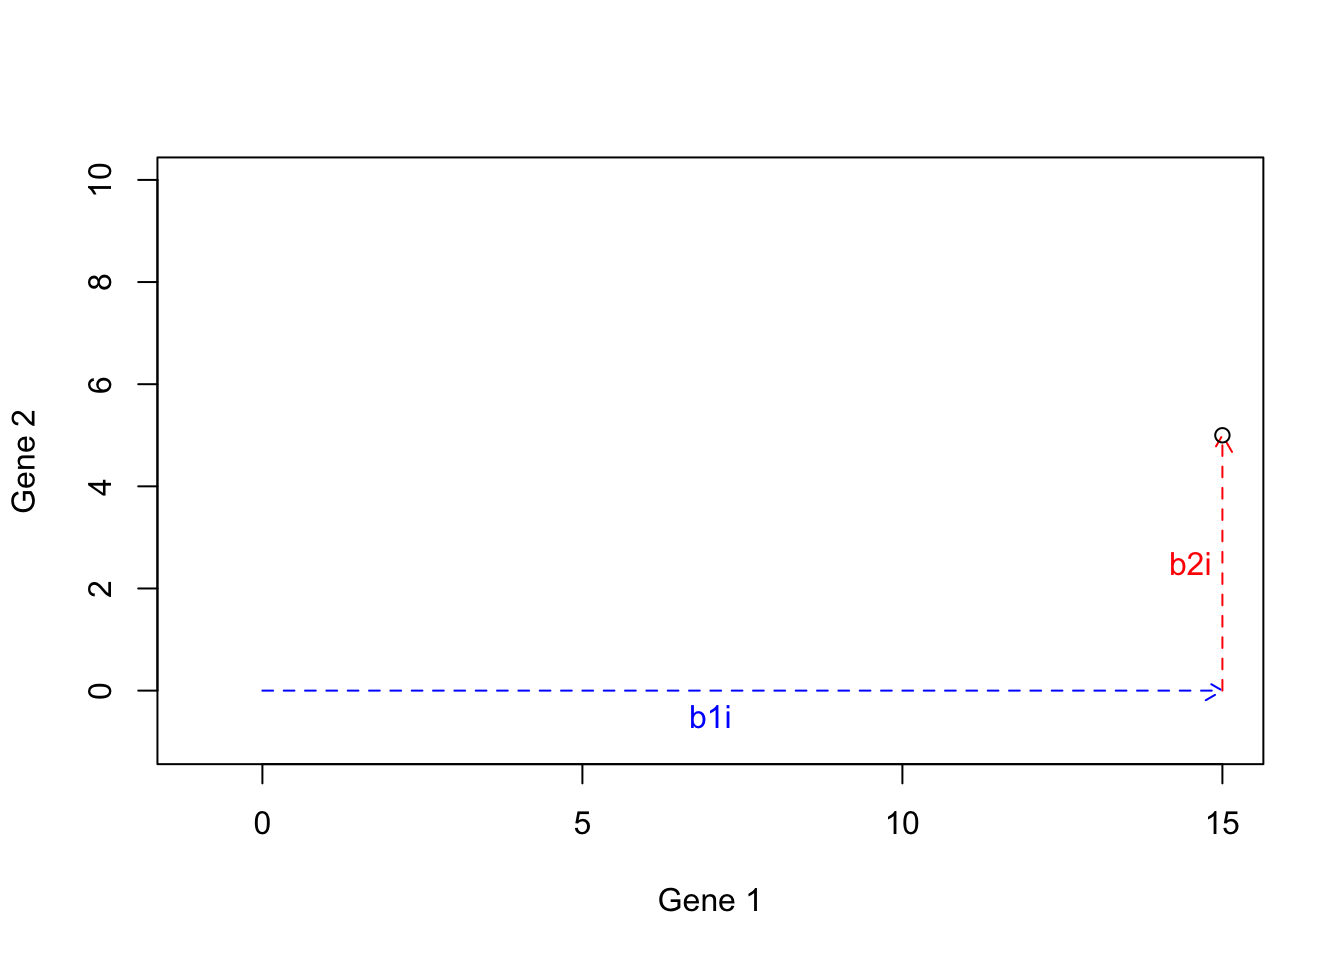
\includegraphics{PCA_files/figure-latex/spaceex20-1} 

}

\caption{Example of basis vectors (b1i+b2i)}\label{fig:spaceex20}
\end{figure}

We can now draw a line from the origin to the tip of \(b1i+b2i\):

\begin{Shaded}
\begin{Highlighting}[]
\KeywordTok{par}\NormalTok{(}\DataTypeTok{mfrow=}\KeywordTok{c}\NormalTok{(}\DecValTok{1}\NormalTok{,}\DecValTok{1}\NormalTok{))}
\CommentTok{# plot}
\KeywordTok{plot}\NormalTok{(}\KeywordTok{c}\NormalTok{(}\OperatorTok{-}\DecValTok{1}\NormalTok{,}\DecValTok{15}\NormalTok{),}\KeywordTok{c}\NormalTok{(}\OperatorTok{-}\DecValTok{1}\NormalTok{,}\DecValTok{10}\NormalTok{),}\DataTypeTok{xlab =} \StringTok{"Gene 1"}\NormalTok{,}\DataTypeTok{ylab =} \StringTok{"Gene 2"}\NormalTok{,}
 \DataTypeTok{axes =}\NormalTok{ T,}\DataTypeTok{type =} \StringTok{"n"}\NormalTok{)}

\KeywordTok{arrows}\NormalTok{(}\DecValTok{0}\NormalTok{,}\DecValTok{0}\NormalTok{,}\DecValTok{15}\NormalTok{,}\DecValTok{0}\NormalTok{,}\DataTypeTok{col=}\StringTok{"blue"}\NormalTok{,}\DataTypeTok{length =} \FloatTok{0.1}\NormalTok{,}\DataTypeTok{lty =} \StringTok{"dashed"}\NormalTok{)}
\KeywordTok{text}\NormalTok{(}\DecValTok{7}\NormalTok{,}\OperatorTok{-}\FloatTok{0.5}\NormalTok{,}\StringTok{"b1i"}\NormalTok{,}\DataTypeTok{col=}\StringTok{"blue"}\NormalTok{)}

\KeywordTok{arrows}\NormalTok{(}\DecValTok{15}\NormalTok{,}\DecValTok{0}\NormalTok{,}\DecValTok{15}\NormalTok{,}\DecValTok{5}\NormalTok{,}\DataTypeTok{col=}\StringTok{"red"}\NormalTok{,}\DataTypeTok{length =} \FloatTok{0.1}\NormalTok{,}\DataTypeTok{lty =} \StringTok{"dashed"}\NormalTok{)}
\KeywordTok{text}\NormalTok{(}\FloatTok{14.5}\NormalTok{,}\FloatTok{2.5}\NormalTok{,}\StringTok{"b2i"}\NormalTok{,}\DataTypeTok{col=}\StringTok{"red"}\NormalTok{)}

\KeywordTok{arrows}\NormalTok{(}\DecValTok{0}\NormalTok{,}\DecValTok{0}\NormalTok{,}\DecValTok{15}\NormalTok{,}\DecValTok{5}\NormalTok{,}\DataTypeTok{col=}\StringTok{"black"}\NormalTok{,}\DataTypeTok{length =} \FloatTok{0.1}\NormalTok{,}\DataTypeTok{lty =} \StringTok{"dashed"}\NormalTok{)}
\KeywordTok{text}\NormalTok{(}\DecValTok{8}\NormalTok{,}\FloatTok{3.5}\NormalTok{,}\StringTok{"h"}\NormalTok{,}\DataTypeTok{col=}\StringTok{"black"}\NormalTok{)}

\KeywordTok{points}\NormalTok{(}\DecValTok{15}\NormalTok{,}\DecValTok{5}\NormalTok{)}
\end{Highlighting}
\end{Shaded}

\begin{figure}

{\centering \includegraphics{PCA_files/figure-latex/spaceex21-1} 

}

\caption{Example of basis vectors (calculating h)}\label{fig:spaceex21}
\end{figure}

I hope that you got the point by now. We can use the basis vectors to construct any vector in our space. In fact, our observations vectors (e.g.~samples) are basis vectors that have been scaled and added.

We come to the end of the vector section. The important point here is that we have been working on two dimensions, all the operations and concept discussed so far can be extend to work in high dimension. Remember our dataset had 45101 dimensions. We have only worked on two of them so far :)

\hypertarget{matrices}{%
\section{Matrices}\label{matrices}}

Matrices can be thought as generalization of vectors where we put multiple vectors together to form a ``table''. You can think about an Excel sheet where each row or each column is vector but the complete sheet is a matrix. We normally store our data in matrices as we showed in Table \ref{tab:tablesample}. As you noticed, matrices have can have columns and rows. These are dimensions of a matrix. In our test data, we dimension is

\begin{Shaded}
\begin{Highlighting}[]
\CommentTok{# show dimensions of the data}
\KeywordTok{dim}\NormalTok{(data)}
\end{Highlighting}
\end{Shaded}

\begin{verbatim}
## [1]    23 45101
\end{verbatim}

Throughout this section, we show matrices with capital letters as opposed to vectors that are shown using small letters.
\[
A=\begin{bmatrix}
1 & 2 & 3\\
4 & 5 & 6
\end{bmatrix}
\]
As you see, we have two rows and three columns. When we want to refer to a specific location (\textbf{called entry}) in the matrix, we use \emph{i} for the row index and \emph{j} for the column index.

For example \(A_{1,2}\) refers to an entry sitting in the \textbf{first} frow and the **second column of the matrix, giving us \(2\).

We refer to the entire row of the matrix by \emph{i,*}. For example, \(A_{2,*}\) will give us \([4,5,6]\). The same way, we can refer to the entire column \(A_{*,2}\), giving us \([2,5]\).

Many of the operations defined for the vectors are also applied on the matrices. We can add or subtract them but the important thing is that the matrices \textbf{MUST} be the same size (same dimensions) to be able to perform addition and subtraction. In the case of addition and subtraction, each entry of the first matrix will be added or substracted to the same entry (same location) in the second matrix:

\[
\begin{bmatrix}
1 & 2 & 3\\
4 & 5 & 6
\end{bmatrix}+
\begin{bmatrix}
7 & 8 & 9\\
10 & 11 & 12
\end{bmatrix}=
\begin{bmatrix}
1+7 & 2+8 & 3+9\\
4+10 & 5+11 & 6+12
\end{bmatrix}
\]
The same applies in scalar multiplication:

\[
5 \times \begin{bmatrix}
1 & 2 & 3\\
4 & 5 & 6
\end{bmatrix}=
\begin{bmatrix}
5 \times 1 & 5 \times 2 & 5 \times 3\\
5 \times 4 & 5 \times 5 & 5 \times 6
\end{bmatrix}
\]
We can think about addition, subtraction and scalar multiplication the same way as the vectors. However, instead of having one vector, we have multiple ones.

For example, if we add \(A=\begin{bmatrix}2&4\\5&3\end{bmatrix}\) and \(B=\begin{bmatrix}4&5\\2&2\end{bmatrix}\) we will get \(C=\begin{bmatrix}6&9\\7&5\end{bmatrix}\). We can think about we have two genes (number of columns) and we have two patients (number of rows) in \(A\) and \(B\). Each patient will give us an arrow.

\begin{Shaded}
\begin{Highlighting}[]
\CommentTok{# }
\KeywordTok{par}\NormalTok{(}\DataTypeTok{mfrow=}\KeywordTok{c}\NormalTok{(}\DecValTok{2}\NormalTok{,}\DecValTok{2}\NormalTok{))}
\CommentTok{# define matrices}
\NormalTok{A<-}\KeywordTok{matrix}\NormalTok{(}\KeywordTok{c}\NormalTok{(}\DecValTok{2}\NormalTok{,}\DecValTok{4}\NormalTok{,}\DecValTok{5}\NormalTok{,}\DecValTok{3}\NormalTok{),}\DataTypeTok{nrow =} \DecValTok{2}\NormalTok{,}\DataTypeTok{ncol =} \DecValTok{2}\NormalTok{,}\DataTypeTok{byrow =}\NormalTok{ T)}

\NormalTok{B<-}\KeywordTok{matrix}\NormalTok{(}\KeywordTok{c}\NormalTok{(}\DecValTok{4}\NormalTok{,}\DecValTok{5}\NormalTok{,}\DecValTok{2}\NormalTok{,}\DecValTok{2}\NormalTok{),}\DataTypeTok{nrow =} \DecValTok{2}\NormalTok{,}\DataTypeTok{ncol =} \DecValTok{2}\NormalTok{,}\DataTypeTok{byrow =}\NormalTok{ T)}

\NormalTok{C=A}\OperatorTok{+}\NormalTok{B}

\CommentTok{# Plot arrows in A}
\KeywordTok{plot}\NormalTok{(}\KeywordTok{c}\NormalTok{(}\DecValTok{0}\NormalTok{,}\DecValTok{10}\NormalTok{),}\KeywordTok{c}\NormalTok{(}\DecValTok{0}\NormalTok{,}\DecValTok{10}\NormalTok{),}\DataTypeTok{xlab =} \StringTok{""}\NormalTok{,}\DataTypeTok{ylab =} \StringTok{""}\NormalTok{,}
 \DataTypeTok{axes =}\NormalTok{ T,}\DataTypeTok{type =} \StringTok{"n"}\NormalTok{)}
\KeywordTok{title}\NormalTok{(}\StringTok{"Matrix A"}\NormalTok{)}

\KeywordTok{arrows}\NormalTok{(}\DecValTok{0}\NormalTok{,}\DecValTok{0}\NormalTok{,A[}\DecValTok{1}\NormalTok{,}\DecValTok{1}\NormalTok{],A[}\DecValTok{1}\NormalTok{,}\DecValTok{2}\NormalTok{],}\DataTypeTok{col=}\StringTok{"blue"}\NormalTok{,}\DataTypeTok{length =} \FloatTok{0.1}\NormalTok{)}
\KeywordTok{text}\NormalTok{(A[}\DecValTok{1}\NormalTok{,}\DecValTok{1}\NormalTok{]}\OperatorTok{/}\DecValTok{2}\NormalTok{,A[}\DecValTok{1}\NormalTok{,}\DecValTok{2}\NormalTok{]}\OperatorTok{/}\DecValTok{2}\NormalTok{,}\KeywordTok{expression}\NormalTok{(}\StringTok{'A'}\NormalTok{[}\StringTok{"1,*"}\NormalTok{]),}\DataTypeTok{col=}\StringTok{"blue"}\NormalTok{,}\DataTypeTok{adj =} \FloatTok{-0.5}\NormalTok{)}

\KeywordTok{arrows}\NormalTok{(}\DecValTok{0}\NormalTok{,}\DecValTok{0}\NormalTok{,A[}\DecValTok{2}\NormalTok{,}\DecValTok{1}\NormalTok{],A[}\DecValTok{2}\NormalTok{,}\DecValTok{2}\NormalTok{],}\DataTypeTok{col=}\StringTok{"red"}\NormalTok{,}\DataTypeTok{length =} \FloatTok{0.1}\NormalTok{)}
\KeywordTok{text}\NormalTok{(A[}\DecValTok{2}\NormalTok{,}\DecValTok{1}\NormalTok{]}\OperatorTok{/}\DecValTok{2}\NormalTok{,A[}\DecValTok{2}\NormalTok{,}\DecValTok{2}\NormalTok{]}\OperatorTok{/}\DecValTok{2}\NormalTok{,}\KeywordTok{expression}\NormalTok{(}\StringTok{'A'}\NormalTok{[}\StringTok{"2,*"}\NormalTok{]),}\DataTypeTok{col=}\StringTok{"red"}\NormalTok{,}\DataTypeTok{adj =} \FloatTok{-0.5}\NormalTok{)}

\CommentTok{# Plot arrows in B}
\KeywordTok{plot}\NormalTok{(}\KeywordTok{c}\NormalTok{(}\DecValTok{0}\NormalTok{,}\DecValTok{10}\NormalTok{),}\KeywordTok{c}\NormalTok{(}\DecValTok{0}\NormalTok{,}\DecValTok{10}\NormalTok{),}\DataTypeTok{xlab =} \StringTok{""}\NormalTok{,}\DataTypeTok{ylab =} \StringTok{""}\NormalTok{,}
 \DataTypeTok{axes =}\NormalTok{ T,}\DataTypeTok{type =} \StringTok{"n"}\NormalTok{)}
\KeywordTok{title}\NormalTok{(}\StringTok{"Matrix B"}\NormalTok{)}

\KeywordTok{arrows}\NormalTok{(}\DecValTok{0}\NormalTok{,}\DecValTok{0}\NormalTok{,B[}\DecValTok{1}\NormalTok{,}\DecValTok{1}\NormalTok{],B[}\DecValTok{1}\NormalTok{,}\DecValTok{2}\NormalTok{],}\DataTypeTok{col=}\StringTok{"green"}\NormalTok{,}\DataTypeTok{length =} \FloatTok{0.1}\NormalTok{)}
\KeywordTok{text}\NormalTok{(B[}\DecValTok{1}\NormalTok{,}\DecValTok{1}\NormalTok{]}\OperatorTok{/}\DecValTok{2}\NormalTok{,B[}\DecValTok{1}\NormalTok{,}\DecValTok{2}\NormalTok{]}\OperatorTok{/}\DecValTok{2}\NormalTok{,}\KeywordTok{expression}\NormalTok{(}\StringTok{'B'}\NormalTok{[}\StringTok{"1,*"}\NormalTok{]),}\DataTypeTok{col=}\StringTok{"green"}\NormalTok{,}\DataTypeTok{adj =} \FloatTok{-0.5}\NormalTok{)}

\KeywordTok{arrows}\NormalTok{(}\DecValTok{0}\NormalTok{,}\DecValTok{0}\NormalTok{,B[}\DecValTok{2}\NormalTok{,}\DecValTok{1}\NormalTok{],B[}\DecValTok{2}\NormalTok{,}\DecValTok{2}\NormalTok{],}\DataTypeTok{col=}\StringTok{"purple"}\NormalTok{,}\DataTypeTok{length =} \FloatTok{0.1}\NormalTok{)}
\KeywordTok{text}\NormalTok{(B[}\DecValTok{2}\NormalTok{,}\DecValTok{1}\NormalTok{]}\OperatorTok{/}\DecValTok{2}\NormalTok{,B[}\DecValTok{2}\NormalTok{,}\DecValTok{2}\NormalTok{]}\OperatorTok{/}\DecValTok{2}\NormalTok{,}\KeywordTok{expression}\NormalTok{(}\StringTok{'B'}\NormalTok{[}\StringTok{"2,*"}\NormalTok{]),}\DataTypeTok{col=}\StringTok{"purple"}\NormalTok{,}\DataTypeTok{adj =} \FloatTok{-0.5}\NormalTok{)}

\CommentTok{# Plot arrows in A+b}
\KeywordTok{plot}\NormalTok{(}\KeywordTok{c}\NormalTok{(}\DecValTok{0}\NormalTok{,}\DecValTok{10}\NormalTok{),}\KeywordTok{c}\NormalTok{(}\DecValTok{0}\NormalTok{,}\DecValTok{10}\NormalTok{),}\DataTypeTok{xlab =} \StringTok{""}\NormalTok{,}\DataTypeTok{ylab =} \StringTok{""}\NormalTok{,}
 \DataTypeTok{axes =}\NormalTok{ T,}\DataTypeTok{type =} \StringTok{"n"}\NormalTok{)}
\KeywordTok{title}\NormalTok{(}\StringTok{"Matrix A+B"}\NormalTok{)}


\KeywordTok{arrows}\NormalTok{(}\DecValTok{0}\NormalTok{,}\DecValTok{0}\NormalTok{,A[}\DecValTok{1}\NormalTok{,}\DecValTok{1}\NormalTok{],A[}\DecValTok{1}\NormalTok{,}\DecValTok{2}\NormalTok{],}\DataTypeTok{col=}\StringTok{"blue"}\NormalTok{,}\DataTypeTok{length =} \FloatTok{0.1}\NormalTok{)}
\KeywordTok{text}\NormalTok{(A[}\DecValTok{1}\NormalTok{,}\DecValTok{1}\NormalTok{]}\OperatorTok{/}\DecValTok{2}\NormalTok{,A[}\DecValTok{1}\NormalTok{,}\DecValTok{2}\NormalTok{]}\OperatorTok{/}\DecValTok{2}\NormalTok{,}\KeywordTok{expression}\NormalTok{(}\StringTok{'A'}\NormalTok{[}\StringTok{"1,*"}\NormalTok{]),}\DataTypeTok{col=}\StringTok{"blue"}\NormalTok{,}\DataTypeTok{adj =} \FloatTok{-0.5}\NormalTok{)}

\KeywordTok{arrows}\NormalTok{(}\DecValTok{0}\NormalTok{,}\DecValTok{0}\NormalTok{,A[}\DecValTok{2}\NormalTok{,}\DecValTok{1}\NormalTok{],A[}\DecValTok{2}\NormalTok{,}\DecValTok{2}\NormalTok{],}\DataTypeTok{col=}\StringTok{"red"}\NormalTok{,}\DataTypeTok{length =} \FloatTok{0.1}\NormalTok{)}
\KeywordTok{text}\NormalTok{(A[}\DecValTok{2}\NormalTok{,}\DecValTok{1}\NormalTok{]}\OperatorTok{/}\DecValTok{2}\NormalTok{,A[}\DecValTok{2}\NormalTok{,}\DecValTok{2}\NormalTok{]}\OperatorTok{/}\DecValTok{2}\NormalTok{,}\KeywordTok{expression}\NormalTok{(}\StringTok{'A'}\NormalTok{[}\StringTok{"2,*"}\NormalTok{]),}\DataTypeTok{col=}\StringTok{"red"}\NormalTok{,}\DataTypeTok{adj =} \FloatTok{-0.5}\NormalTok{)}


\KeywordTok{arrows}\NormalTok{(A[}\DecValTok{1}\NormalTok{,}\DecValTok{1}\NormalTok{],A[}\DecValTok{1}\NormalTok{,}\DecValTok{2}\NormalTok{],C[}\DecValTok{1}\NormalTok{,}\DecValTok{1}\NormalTok{],C[}\DecValTok{1}\NormalTok{,}\DecValTok{2}\NormalTok{],}\DataTypeTok{col=}\StringTok{"green"}\NormalTok{,}\DataTypeTok{length =} \FloatTok{0.1}\NormalTok{,}\DataTypeTok{lty =} \StringTok{"dashed"}\NormalTok{)}
\KeywordTok{text}\NormalTok{(C[}\DecValTok{1}\NormalTok{,}\DecValTok{1}\NormalTok{]}\OperatorTok{/}\DecValTok{2}\NormalTok{,C[}\DecValTok{1}\NormalTok{,}\DecValTok{2}\NormalTok{]}\OperatorTok{/}\DecValTok{2}\NormalTok{,(}\KeywordTok{expression}\NormalTok{(}\StringTok{'B'}\NormalTok{[}\StringTok{"1,*"}\NormalTok{])),}\DataTypeTok{col=}\StringTok{"green"}\NormalTok{)}

\KeywordTok{arrows}\NormalTok{(A[}\DecValTok{2}\NormalTok{,}\DecValTok{1}\NormalTok{],A[}\DecValTok{2}\NormalTok{,}\DecValTok{2}\NormalTok{],C[}\DecValTok{2}\NormalTok{,}\DecValTok{1}\NormalTok{],C[}\DecValTok{2}\NormalTok{,}\DecValTok{2}\NormalTok{],}\DataTypeTok{col=}\StringTok{"purple"}\NormalTok{,}\DataTypeTok{length =} \FloatTok{0.1}\NormalTok{,}\DataTypeTok{lty =} \StringTok{"dashed"}\NormalTok{)}
\KeywordTok{text}\NormalTok{(C[}\DecValTok{2}\NormalTok{,}\DecValTok{1}\NormalTok{]}\OperatorTok{/}\DecValTok{2}\NormalTok{,C[}\DecValTok{2}\NormalTok{,}\DecValTok{2}\NormalTok{]}\OperatorTok{/}\DecValTok{2}\NormalTok{,(}\KeywordTok{expression}\NormalTok{(}\StringTok{'B'}\NormalTok{[}\StringTok{"2,*"}\NormalTok{])),}\DataTypeTok{col=}\StringTok{"purple"}\NormalTok{,}\DataTypeTok{adj =} \DecValTok{-2}\NormalTok{)}


\CommentTok{## plot C}
\KeywordTok{plot}\NormalTok{(}\KeywordTok{c}\NormalTok{(}\DecValTok{0}\NormalTok{,}\DecValTok{10}\NormalTok{),}\KeywordTok{c}\NormalTok{(}\DecValTok{0}\NormalTok{,}\DecValTok{10}\NormalTok{),}\DataTypeTok{xlab =} \StringTok{""}\NormalTok{,}\DataTypeTok{ylab =} \StringTok{""}\NormalTok{,}
 \DataTypeTok{axes =}\NormalTok{ T,}\DataTypeTok{type =} \StringTok{"n"}\NormalTok{)}
\KeywordTok{title}\NormalTok{(}\StringTok{"Matrix C"}\NormalTok{)}
\KeywordTok{arrows}\NormalTok{(}\DecValTok{0}\NormalTok{,}\DecValTok{0}\NormalTok{,C[}\DecValTok{1}\NormalTok{,}\DecValTok{1}\NormalTok{],C[}\DecValTok{1}\NormalTok{,}\DecValTok{2}\NormalTok{],}\DataTypeTok{col=}\StringTok{"blue"}\NormalTok{,}\DataTypeTok{length =} \FloatTok{0.1}\NormalTok{)}
\KeywordTok{text}\NormalTok{(C[}\DecValTok{1}\NormalTok{,}\DecValTok{1}\NormalTok{]}\OperatorTok{/}\DecValTok{2}\NormalTok{,C[}\DecValTok{1}\NormalTok{,}\DecValTok{2}\NormalTok{]}\OperatorTok{/}\DecValTok{2}\NormalTok{,}\KeywordTok{expression}\NormalTok{(}\StringTok{'C'}\NormalTok{[}\StringTok{"1,*"}\NormalTok{]),}\DataTypeTok{col=}\StringTok{"blue"}\NormalTok{,}\DataTypeTok{adj =} \FloatTok{-0.5}\NormalTok{)}

\KeywordTok{arrows}\NormalTok{(}\DecValTok{0}\NormalTok{,}\DecValTok{0}\NormalTok{,C[}\DecValTok{2}\NormalTok{,}\DecValTok{1}\NormalTok{],C[}\DecValTok{2}\NormalTok{,}\DecValTok{2}\NormalTok{],}\DataTypeTok{col=}\StringTok{"red"}\NormalTok{,}\DataTypeTok{length =} \FloatTok{0.1}\NormalTok{)}
\KeywordTok{text}\NormalTok{(C[}\DecValTok{2}\NormalTok{,}\DecValTok{1}\NormalTok{]}\OperatorTok{/}\DecValTok{2}\NormalTok{,C[}\DecValTok{2}\NormalTok{,}\DecValTok{2}\NormalTok{]}\OperatorTok{/}\DecValTok{2}\NormalTok{,}\KeywordTok{expression}\NormalTok{(}\StringTok{'C'}\NormalTok{[}\StringTok{"2,*"}\NormalTok{]),}\DataTypeTok{col=}\StringTok{"red"}\NormalTok{,}\DataTypeTok{adj =} \FloatTok{-0.5}\NormalTok{)}
\end{Highlighting}
\end{Shaded}

\begin{figure}

{\centering \includegraphics{PCA_files/figure-latex/matrix1-1} 

}

\caption{Example of matrix addition}\label{fig:matrix1}
\end{figure}

So what we see in Figure \ref{fig:matrix1} is that, we have two matrices A and B, we take the vectors in B and put them at the tip of the vectors in A, we then draw two lines from the origin to the new tips of B. So as it's obvious now, this is the same and vector addition we just do it for more vectors.

\hypertarget{matrix-multiplication}{%
\subsection{Matrix multiplication}\label{matrix-multiplication}}

In order to understand matrix multiplication, we have to think about the space again. \protect\hyperlink{bvectors}{If you remember}, we said the we can represent our space by the basis vector \(\vec{x}=[1,0]\) and \(\vec{y}=[0,1]\). We can think about this as directions or our guide to move to any points in the space. We said that we can scale them, we can add/subtract them to represent any vectors in the space. Our space is an empty huge place wherein we just put our vectors! The way that we navigate in space, is just by scaling and adding and subtracting the basis vectors. I keep repeating this because it's important to understand it thoroughly. So let's have a look at our empty space (well, i just put the grid so we have feeling of it)

\begin{Shaded}
\begin{Highlighting}[]
\KeywordTok{par}\NormalTok{(}\DataTypeTok{mfrow=}\KeywordTok{c}\NormalTok{(}\DecValTok{1}\NormalTok{,}\DecValTok{1}\NormalTok{))}

\NormalTok{mydata<-}\KeywordTok{cbind}\NormalTok{(}\OperatorTok{-}\DecValTok{5}\OperatorTok{:}\DecValTok{5}\NormalTok{,}\KeywordTok{rep}\NormalTok{(}\OperatorTok{-}\DecValTok{5}\NormalTok{,}\DecValTok{11}\NormalTok{),}\OperatorTok{-}\DecValTok{5}\OperatorTok{:}\DecValTok{5}\NormalTok{,}\KeywordTok{rep}\NormalTok{(}\DecValTok{5}\NormalTok{,}\DecValTok{11}\NormalTok{))}

\NormalTok{mydata2<-}\KeywordTok{cbind}\NormalTok{(}\KeywordTok{rep}\NormalTok{(}\OperatorTok{-}\DecValTok{5}\NormalTok{,}\DecValTok{11}\NormalTok{),}\OperatorTok{-}\DecValTok{5}\OperatorTok{:}\DecValTok{5}\NormalTok{,}\KeywordTok{rep}\NormalTok{(}\DecValTok{5}\NormalTok{,}\DecValTok{11}\NormalTok{),}\OperatorTok{-}\DecValTok{5}\OperatorTok{:}\DecValTok{5}\NormalTok{)}

\KeywordTok{plot}\NormalTok{(}\KeywordTok{range}\NormalTok{(}\KeywordTok{rbind}\NormalTok{(mydata[,}\DecValTok{1}\NormalTok{],mydata[,}\DecValTok{3}\NormalTok{])),}\KeywordTok{range}\NormalTok{(}\KeywordTok{rbind}\NormalTok{(mydata[,}\DecValTok{2}\NormalTok{],mydata[,}\DecValTok{4}\NormalTok{])),}
     \DataTypeTok{type=}\StringTok{"n"}\NormalTok{,}\DataTypeTok{xlab=}\StringTok{""}\NormalTok{,}\DataTypeTok{ylab=}\StringTok{""}\NormalTok{,}\DataTypeTok{xlim=}\KeywordTok{c}\NormalTok{(}\OperatorTok{-}\DecValTok{5}\NormalTok{,}\DecValTok{5}\NormalTok{),}\DataTypeTok{ylim=}\KeywordTok{c}\NormalTok{(}\OperatorTok{-}\DecValTok{5}\NormalTok{,}\DecValTok{5}\NormalTok{),}\DataTypeTok{axes =}\NormalTok{ F,}\DataTypeTok{bg=}\StringTok{"black"}\NormalTok{)}


\NormalTok{nl<-}\KeywordTok{apply}\NormalTok{(mydata,}\DataTypeTok{MARGIN =} \DecValTok{1}\NormalTok{,}\ControlFlowTok{function}\NormalTok{(x)\{}
  \KeywordTok{segments}\NormalTok{(x[}\DecValTok{1}\NormalTok{],x[}\DecValTok{2}\NormalTok{],x[}\DecValTok{3}\NormalTok{],x[}\DecValTok{4}\NormalTok{])\})}

\NormalTok{nl<-}\KeywordTok{apply}\NormalTok{(mydata2,}\DataTypeTok{MARGIN =} \DecValTok{1}\NormalTok{,}\ControlFlowTok{function}\NormalTok{(x)\{}
  \KeywordTok{segments}\NormalTok{(x[}\DecValTok{1}\NormalTok{],x[}\DecValTok{2}\NormalTok{],x[}\DecValTok{3}\NormalTok{],x[}\DecValTok{4}\NormalTok{])\})}


\KeywordTok{arrows}\NormalTok{(}\DecValTok{0}\NormalTok{,}\DecValTok{0}\NormalTok{,}\DecValTok{1}\NormalTok{,}\DecValTok{0}\NormalTok{,}\DataTypeTok{col=}\StringTok{"red"}\NormalTok{,}\DataTypeTok{length=}\FloatTok{0.1}\NormalTok{)}
\KeywordTok{arrows}\NormalTok{(}\DecValTok{0}\NormalTok{,}\DecValTok{0}\NormalTok{,}\DecValTok{0}\NormalTok{,}\DecValTok{1}\NormalTok{,}\DataTypeTok{col=}\StringTok{"blue"}\NormalTok{,}\DataTypeTok{length=}\FloatTok{0.1}\NormalTok{)}
\end{Highlighting}
\end{Shaded}

\begin{figure}

{\centering \includegraphics{PCA_files/figure-latex/matrix2-1} 

}

\caption{Empty space}\label{fig:matrix2}
\end{figure}

We can go to any point on this grid, simply using our basis vectors.

\begin{Shaded}
\begin{Highlighting}[]
\KeywordTok{par}\NormalTok{(}\DataTypeTok{mfrow=}\KeywordTok{c}\NormalTok{(}\DecValTok{1}\NormalTok{,}\DecValTok{1}\NormalTok{))}

\NormalTok{mydata<-}\KeywordTok{cbind}\NormalTok{(}\OperatorTok{-}\DecValTok{5}\OperatorTok{:}\DecValTok{5}\NormalTok{,}\KeywordTok{rep}\NormalTok{(}\OperatorTok{-}\DecValTok{5}\NormalTok{,}\DecValTok{11}\NormalTok{),}\OperatorTok{-}\DecValTok{5}\OperatorTok{:}\DecValTok{5}\NormalTok{,}\KeywordTok{rep}\NormalTok{(}\DecValTok{5}\NormalTok{,}\DecValTok{11}\NormalTok{))}

\NormalTok{mydata2<-}\KeywordTok{cbind}\NormalTok{(}\KeywordTok{rep}\NormalTok{(}\OperatorTok{-}\DecValTok{5}\NormalTok{,}\DecValTok{11}\NormalTok{),}\OperatorTok{-}\DecValTok{5}\OperatorTok{:}\DecValTok{5}\NormalTok{,}\KeywordTok{rep}\NormalTok{(}\DecValTok{5}\NormalTok{,}\DecValTok{11}\NormalTok{),}\OperatorTok{-}\DecValTok{5}\OperatorTok{:}\DecValTok{5}\NormalTok{)}

\KeywordTok{plot}\NormalTok{(}\KeywordTok{range}\NormalTok{(}\KeywordTok{rbind}\NormalTok{(mydata[,}\DecValTok{1}\NormalTok{],mydata[,}\DecValTok{3}\NormalTok{])),}\KeywordTok{range}\NormalTok{(}\KeywordTok{rbind}\NormalTok{(mydata[,}\DecValTok{2}\NormalTok{],mydata[,}\DecValTok{4}\NormalTok{])),}
     \DataTypeTok{type=}\StringTok{"n"}\NormalTok{,}\DataTypeTok{xlab=}\StringTok{""}\NormalTok{,}\DataTypeTok{ylab=}\StringTok{""}\NormalTok{,}\DataTypeTok{xlim=}\KeywordTok{c}\NormalTok{(}\OperatorTok{-}\DecValTok{5}\NormalTok{,}\DecValTok{5}\NormalTok{),}\DataTypeTok{ylim=}\KeywordTok{c}\NormalTok{(}\OperatorTok{-}\DecValTok{5}\NormalTok{,}\DecValTok{5}\NormalTok{),}\DataTypeTok{axes =}\NormalTok{ F,}\DataTypeTok{bg=}\StringTok{"black"}\NormalTok{)}


\NormalTok{nl<-}\KeywordTok{apply}\NormalTok{(mydata,}\DataTypeTok{MARGIN =} \DecValTok{1}\NormalTok{,}\ControlFlowTok{function}\NormalTok{(x)\{}
  \KeywordTok{segments}\NormalTok{(x[}\DecValTok{1}\NormalTok{],x[}\DecValTok{2}\NormalTok{],x[}\DecValTok{3}\NormalTok{],x[}\DecValTok{4}\NormalTok{])\})}

\NormalTok{nl<-}\KeywordTok{apply}\NormalTok{(mydata2,}\DataTypeTok{MARGIN =} \DecValTok{1}\NormalTok{,}\ControlFlowTok{function}\NormalTok{(x)\{}
  \KeywordTok{segments}\NormalTok{(x[}\DecValTok{1}\NormalTok{],x[}\DecValTok{2}\NormalTok{],x[}\DecValTok{3}\NormalTok{],x[}\DecValTok{4}\NormalTok{])\})}


\KeywordTok{arrows}\NormalTok{(}\DecValTok{0}\NormalTok{,}\DecValTok{0}\NormalTok{,}\DecValTok{1}\NormalTok{,}\DecValTok{0}\NormalTok{,}\DataTypeTok{col=}\StringTok{"red"}\NormalTok{,}\DataTypeTok{length=}\FloatTok{0.1}\NormalTok{)}
\KeywordTok{arrows}\NormalTok{(}\DecValTok{0}\NormalTok{,}\DecValTok{0}\NormalTok{,}\DecValTok{0}\NormalTok{,}\DecValTok{1}\NormalTok{,}\DataTypeTok{col=}\StringTok{"blue"}\NormalTok{,}\DataTypeTok{length=}\FloatTok{0.1}\NormalTok{)}

\KeywordTok{points}\NormalTok{(}\DecValTok{4}\NormalTok{,}\DecValTok{3}\NormalTok{,}\DataTypeTok{col=}\StringTok{"purple"}\NormalTok{,}\DataTypeTok{pch=}\DecValTok{7}\NormalTok{)}
\end{Highlighting}
\end{Shaded}

\begin{figure}

{\centering \includegraphics{PCA_files/figure-latex/matrix3-1} 

}

\caption{Empty space and a target point}\label{fig:matrix3}
\end{figure}

Remember now, this target point can be an observation (e.g.~sample etc). We can move to this point simply by multiplying \(\vec{x}\) to 4 and \(\vec{y}\) to 3 and then add the resulting vectors, giving us the location of the purple point \([4,3]\).

\begin{Shaded}
\begin{Highlighting}[]
\KeywordTok{par}\NormalTok{(}\DataTypeTok{mfrow=}\KeywordTok{c}\NormalTok{(}\DecValTok{1}\NormalTok{,}\DecValTok{1}\NormalTok{))}

\NormalTok{mydata<-}\KeywordTok{cbind}\NormalTok{(}\OperatorTok{-}\DecValTok{5}\OperatorTok{:}\DecValTok{5}\NormalTok{,}\KeywordTok{rep}\NormalTok{(}\OperatorTok{-}\DecValTok{5}\NormalTok{,}\DecValTok{11}\NormalTok{),}\OperatorTok{-}\DecValTok{5}\OperatorTok{:}\DecValTok{5}\NormalTok{,}\KeywordTok{rep}\NormalTok{(}\DecValTok{5}\NormalTok{,}\DecValTok{11}\NormalTok{))}

\NormalTok{mydata2<-}\KeywordTok{cbind}\NormalTok{(}\KeywordTok{rep}\NormalTok{(}\OperatorTok{-}\DecValTok{5}\NormalTok{,}\DecValTok{11}\NormalTok{),}\OperatorTok{-}\DecValTok{5}\OperatorTok{:}\DecValTok{5}\NormalTok{,}\KeywordTok{rep}\NormalTok{(}\DecValTok{5}\NormalTok{,}\DecValTok{11}\NormalTok{),}\OperatorTok{-}\DecValTok{5}\OperatorTok{:}\DecValTok{5}\NormalTok{)}

\KeywordTok{plot}\NormalTok{(}\KeywordTok{range}\NormalTok{(}\KeywordTok{rbind}\NormalTok{(mydata[,}\DecValTok{1}\NormalTok{],mydata[,}\DecValTok{3}\NormalTok{])),}\KeywordTok{range}\NormalTok{(}\KeywordTok{rbind}\NormalTok{(mydata[,}\DecValTok{2}\NormalTok{],mydata[,}\DecValTok{4}\NormalTok{])),}
     \DataTypeTok{type=}\StringTok{"n"}\NormalTok{,}\DataTypeTok{xlab=}\StringTok{""}\NormalTok{,}\DataTypeTok{ylab=}\StringTok{""}\NormalTok{,}\DataTypeTok{xlim=}\KeywordTok{c}\NormalTok{(}\OperatorTok{-}\DecValTok{8}\NormalTok{,}\DecValTok{8}\NormalTok{),}\DataTypeTok{ylim=}\KeywordTok{c}\NormalTok{(}\OperatorTok{-}\DecValTok{8}\NormalTok{,}\DecValTok{8}\NormalTok{),}\DataTypeTok{axes =}\NormalTok{ F,}\DataTypeTok{bg=}\StringTok{"black"}\NormalTok{)}


\NormalTok{nl<-}\KeywordTok{apply}\NormalTok{(mydata,}\DataTypeTok{MARGIN =} \DecValTok{1}\NormalTok{,}\ControlFlowTok{function}\NormalTok{(x)\{}
  \KeywordTok{segments}\NormalTok{(x[}\DecValTok{1}\NormalTok{],x[}\DecValTok{2}\NormalTok{],x[}\DecValTok{3}\NormalTok{],x[}\DecValTok{4}\NormalTok{])\})}

\NormalTok{nl<-}\KeywordTok{apply}\NormalTok{(mydata2,}\DataTypeTok{MARGIN =} \DecValTok{1}\NormalTok{,}\ControlFlowTok{function}\NormalTok{(x)\{}
  \KeywordTok{segments}\NormalTok{(x[}\DecValTok{1}\NormalTok{],x[}\DecValTok{2}\NormalTok{],x[}\DecValTok{3}\NormalTok{],x[}\DecValTok{4}\NormalTok{])\})}


\KeywordTok{arrows}\NormalTok{(}\DecValTok{0}\NormalTok{,}\DecValTok{0}\NormalTok{,}\DecValTok{1}\NormalTok{,}\DecValTok{0}\NormalTok{,}\DataTypeTok{col=}\StringTok{"red"}\NormalTok{,}\DataTypeTok{length=}\FloatTok{0.1}\NormalTok{,)}
\KeywordTok{arrows}\NormalTok{(}\DecValTok{0}\NormalTok{,}\DecValTok{0}\NormalTok{,}\DecValTok{0}\NormalTok{,}\DecValTok{1}\NormalTok{,}\DataTypeTok{col=}\StringTok{"blue"}\NormalTok{,}\DataTypeTok{length=}\FloatTok{0.1}\NormalTok{)}

\KeywordTok{points}\NormalTok{(}\DecValTok{4}\NormalTok{,}\DecValTok{3}\NormalTok{,}\DataTypeTok{col=}\StringTok{"purple"}\NormalTok{,}\DataTypeTok{pch=}\DecValTok{7}\NormalTok{)}
\KeywordTok{arrows}\NormalTok{(}\DecValTok{0}\NormalTok{,}\DecValTok{0}\NormalTok{,}\DecValTok{4}\NormalTok{,}\DecValTok{3}\NormalTok{,}\DataTypeTok{col=}\StringTok{"purple"}\NormalTok{,}\DataTypeTok{length=}\FloatTok{0.1}\NormalTok{)}
\end{Highlighting}
\end{Shaded}

\begin{figure}

{\centering \includegraphics{PCA_files/figure-latex/matrix4-1} 

}

\caption{Empty space and a target point}\label{fig:matrix4}
\end{figure}

So far we have only changed the vectors. But we can also change the space itself. If we multiply a matrix to the space itself, we change the space. You can think about this like stretching, squeezing etc applied on the whole grid and ALL the things on that grid. It might not be very understandable in the beginning. Let's have a look an example.

\begin{Shaded}
\begin{Highlighting}[]
\KeywordTok{par}\NormalTok{(}\DataTypeTok{mfrow=}\KeywordTok{c}\NormalTok{(}\DecValTok{1}\NormalTok{,}\DecValTok{1}\NormalTok{))}

\NormalTok{mydata<-}\KeywordTok{cbind}\NormalTok{(}\OperatorTok{-}\DecValTok{5}\OperatorTok{:}\DecValTok{5}\NormalTok{,}\KeywordTok{rep}\NormalTok{(}\OperatorTok{-}\DecValTok{5}\NormalTok{,}\DecValTok{11}\NormalTok{),}\OperatorTok{-}\DecValTok{5}\OperatorTok{:}\DecValTok{5}\NormalTok{,}\KeywordTok{rep}\NormalTok{(}\DecValTok{5}\NormalTok{,}\DecValTok{11}\NormalTok{))}

\NormalTok{mydata2<-}\KeywordTok{cbind}\NormalTok{(}\KeywordTok{rep}\NormalTok{(}\OperatorTok{-}\DecValTok{5}\NormalTok{,}\DecValTok{11}\NormalTok{),}\OperatorTok{-}\DecValTok{5}\OperatorTok{:}\DecValTok{5}\NormalTok{,}\KeywordTok{rep}\NormalTok{(}\DecValTok{5}\NormalTok{,}\DecValTok{11}\NormalTok{),}\OperatorTok{-}\DecValTok{5}\OperatorTok{:}\DecValTok{5}\NormalTok{)}

\KeywordTok{plot}\NormalTok{(}\KeywordTok{range}\NormalTok{(}\KeywordTok{rbind}\NormalTok{(mydata[,}\DecValTok{1}\NormalTok{],mydata[,}\DecValTok{3}\NormalTok{])),}\KeywordTok{range}\NormalTok{(}\KeywordTok{rbind}\NormalTok{(mydata[,}\DecValTok{2}\NormalTok{],mydata[,}\DecValTok{4}\NormalTok{])),}
     \DataTypeTok{type=}\StringTok{"n"}\NormalTok{,}\DataTypeTok{xlab=}\StringTok{""}\NormalTok{,}\DataTypeTok{ylab=}\StringTok{""}\NormalTok{,}\DataTypeTok{xlim=}\KeywordTok{c}\NormalTok{(}\OperatorTok{-}\DecValTok{8}\NormalTok{,}\DecValTok{8}\NormalTok{),}\DataTypeTok{ylim=}\KeywordTok{c}\NormalTok{(}\OperatorTok{-}\DecValTok{8}\NormalTok{,}\DecValTok{8}\NormalTok{),}\DataTypeTok{axes =}\NormalTok{ F,}\DataTypeTok{bg=}\StringTok{"black"}\NormalTok{)}


\NormalTok{b<-}\KeywordTok{as.matrix}\NormalTok{(}\KeywordTok{data.frame}\NormalTok{(}\DataTypeTok{a=}\KeywordTok{c}\NormalTok{(}\DecValTok{1}\NormalTok{,}\DecValTok{0}\NormalTok{),}\DataTypeTok{b=}\KeywordTok{c}\NormalTok{(}\DecValTok{1}\NormalTok{,}\DecValTok{2}\NormalTok{)))}

\NormalTok{mydata[,}\KeywordTok{c}\NormalTok{(}\DecValTok{1}\NormalTok{,}\DecValTok{2}\NormalTok{)]<-}\KeywordTok{t}\NormalTok{(b}\OperatorTok\KeywordTok{t}\NormalTok{(mydata[,}\KeywordTok{c}\NormalTok{(}\DecValTok{1}\NormalTok{,}\DecValTok{2}\NormalTok{)]))}
\NormalTok{mydata[,}\KeywordTok{c}\NormalTok{(}\DecValTok{3}\NormalTok{,}\DecValTok{4}\NormalTok{)]<-}\KeywordTok{t}\NormalTok{(b}\OperatorTok\KeywordTok{t}\NormalTok{(mydata[,}\KeywordTok{c}\NormalTok{(}\DecValTok{3}\NormalTok{,}\DecValTok{4}\NormalTok{)]))}

\NormalTok{mydata2[,}\KeywordTok{c}\NormalTok{(}\DecValTok{1}\NormalTok{,}\DecValTok{2}\NormalTok{)]<-}\KeywordTok{t}\NormalTok{(b}\OperatorTok\KeywordTok{t}\NormalTok{(mydata2[,}\KeywordTok{c}\NormalTok{(}\DecValTok{1}\NormalTok{,}\DecValTok{2}\NormalTok{)]))}
\NormalTok{mydata2[,}\KeywordTok{c}\NormalTok{(}\DecValTok{3}\NormalTok{,}\DecValTok{4}\NormalTok{)]<-}\KeywordTok{t}\NormalTok{(b}\OperatorTok\KeywordTok{t}\NormalTok{(mydata2[,}\KeywordTok{c}\NormalTok{(}\DecValTok{3}\NormalTok{,}\DecValTok{4}\NormalTok{)]))}

\NormalTok{nl<-}\KeywordTok{apply}\NormalTok{(mydata,}\DataTypeTok{MARGIN =} \DecValTok{1}\NormalTok{,}\ControlFlowTok{function}\NormalTok{(x)\{}
  \KeywordTok{segments}\NormalTok{(x[}\DecValTok{1}\NormalTok{],x[}\DecValTok{2}\NormalTok{],x[}\DecValTok{3}\NormalTok{],x[}\DecValTok{4}\NormalTok{])\})}

\NormalTok{nl<-}\KeywordTok{apply}\NormalTok{(mydata2,}\DataTypeTok{MARGIN =} \DecValTok{1}\NormalTok{,}\ControlFlowTok{function}\NormalTok{(x)\{}
  \KeywordTok{segments}\NormalTok{(x[}\DecValTok{1}\NormalTok{],x[}\DecValTok{2}\NormalTok{],x[}\DecValTok{3}\NormalTok{],x[}\DecValTok{4}\NormalTok{])\})}
\end{Highlighting}
\end{Shaded}

\begin{figure}

{\centering \includegraphics{PCA_files/figure-latex/matrix5-1} 

}

\caption{Multiply a matrix to space}\label{fig:matrix5}
\end{figure}

In figure \ref{fig:matrix5}, we multiply \(\begin{bmatrix}1&1\\0&2\end{bmatrix}\) to our space. Please remember, we agreed before that our space was defined by \(\vec{x}=[1,0]\) and \(\vec{y}=[0,1]\) and for clarification, we plotted all the parallel lines (grid) to \(\vec{x}=[1,0]\) and \(\vec{y}=[0,1]\). Isn't this awesome?! We can transform the space itself. We are in a transformed world! How do we find the new address (location) of the previous point (the purple one) in this new world? Well, the only thing we need, is our guides. The new location of the basis vectors. Once we get them, we can use them to find the new address. Let's find them:

\begin{Shaded}
\begin{Highlighting}[]
\KeywordTok{par}\NormalTok{(}\DataTypeTok{mfrow=}\KeywordTok{c}\NormalTok{(}\DecValTok{1}\NormalTok{,}\DecValTok{1}\NormalTok{))}

\NormalTok{mydata<-}\KeywordTok{cbind}\NormalTok{(}\OperatorTok{-}\DecValTok{5}\OperatorTok{:}\DecValTok{5}\NormalTok{,}\KeywordTok{rep}\NormalTok{(}\OperatorTok{-}\DecValTok{5}\NormalTok{,}\DecValTok{11}\NormalTok{),}\OperatorTok{-}\DecValTok{5}\OperatorTok{:}\DecValTok{5}\NormalTok{,}\KeywordTok{rep}\NormalTok{(}\DecValTok{5}\NormalTok{,}\DecValTok{11}\NormalTok{))}

\NormalTok{mydata2<-}\KeywordTok{cbind}\NormalTok{(}\KeywordTok{rep}\NormalTok{(}\OperatorTok{-}\DecValTok{5}\NormalTok{,}\DecValTok{11}\NormalTok{),}\OperatorTok{-}\DecValTok{5}\OperatorTok{:}\DecValTok{5}\NormalTok{,}\KeywordTok{rep}\NormalTok{(}\DecValTok{5}\NormalTok{,}\DecValTok{11}\NormalTok{),}\OperatorTok{-}\DecValTok{5}\OperatorTok{:}\DecValTok{5}\NormalTok{)}

\KeywordTok{plot}\NormalTok{(}\KeywordTok{range}\NormalTok{(}\KeywordTok{rbind}\NormalTok{(mydata[,}\DecValTok{1}\NormalTok{],mydata[,}\DecValTok{3}\NormalTok{])),}\KeywordTok{range}\NormalTok{(}\KeywordTok{rbind}\NormalTok{(mydata[,}\DecValTok{2}\NormalTok{],mydata[,}\DecValTok{4}\NormalTok{])),}
     \DataTypeTok{type=}\StringTok{"n"}\NormalTok{,}\DataTypeTok{xlab=}\StringTok{""}\NormalTok{,}\DataTypeTok{ylab=}\StringTok{""}\NormalTok{,}\DataTypeTok{xlim=}\KeywordTok{c}\NormalTok{(}\OperatorTok{-}\DecValTok{8}\NormalTok{,}\DecValTok{8}\NormalTok{),}\DataTypeTok{ylim=}\KeywordTok{c}\NormalTok{(}\OperatorTok{-}\DecValTok{8}\NormalTok{,}\DecValTok{8}\NormalTok{),}\DataTypeTok{axes =}\NormalTok{ F,}\DataTypeTok{bg=}\StringTok{"black"}\NormalTok{)}


\NormalTok{b<-}\KeywordTok{as.matrix}\NormalTok{(}\KeywordTok{data.frame}\NormalTok{(}\DataTypeTok{a=}\KeywordTok{c}\NormalTok{(}\DecValTok{1}\NormalTok{,}\DecValTok{0}\NormalTok{),}\DataTypeTok{b=}\KeywordTok{c}\NormalTok{(}\DecValTok{1}\NormalTok{,}\DecValTok{2}\NormalTok{)))}

\NormalTok{mydata[,}\KeywordTok{c}\NormalTok{(}\DecValTok{1}\NormalTok{,}\DecValTok{2}\NormalTok{)]<-}\KeywordTok{t}\NormalTok{(b}\OperatorTok\KeywordTok{t}\NormalTok{(mydata[,}\KeywordTok{c}\NormalTok{(}\DecValTok{1}\NormalTok{,}\DecValTok{2}\NormalTok{)]))}
\NormalTok{mydata[,}\KeywordTok{c}\NormalTok{(}\DecValTok{3}\NormalTok{,}\DecValTok{4}\NormalTok{)]<-}\KeywordTok{t}\NormalTok{(b}\OperatorTok\KeywordTok{t}\NormalTok{(mydata[,}\KeywordTok{c}\NormalTok{(}\DecValTok{3}\NormalTok{,}\DecValTok{4}\NormalTok{)]))}

\NormalTok{mydata2[,}\KeywordTok{c}\NormalTok{(}\DecValTok{1}\NormalTok{,}\DecValTok{2}\NormalTok{)]<-}\KeywordTok{t}\NormalTok{(b}\OperatorTok\KeywordTok{t}\NormalTok{(mydata2[,}\KeywordTok{c}\NormalTok{(}\DecValTok{1}\NormalTok{,}\DecValTok{2}\NormalTok{)]))}
\NormalTok{mydata2[,}\KeywordTok{c}\NormalTok{(}\DecValTok{3}\NormalTok{,}\DecValTok{4}\NormalTok{)]<-}\KeywordTok{t}\NormalTok{(b}\OperatorTok\KeywordTok{t}\NormalTok{(mydata2[,}\KeywordTok{c}\NormalTok{(}\DecValTok{3}\NormalTok{,}\DecValTok{4}\NormalTok{)]))}

\NormalTok{nl<-}\KeywordTok{apply}\NormalTok{(mydata,}\DataTypeTok{MARGIN =} \DecValTok{1}\NormalTok{,}\ControlFlowTok{function}\NormalTok{(x)\{}
  \KeywordTok{segments}\NormalTok{(x[}\DecValTok{1}\NormalTok{],x[}\DecValTok{2}\NormalTok{],x[}\DecValTok{3}\NormalTok{],x[}\DecValTok{4}\NormalTok{])\})}

\NormalTok{nl<-}\KeywordTok{apply}\NormalTok{(mydata2,}\DataTypeTok{MARGIN =} \DecValTok{1}\NormalTok{,}\ControlFlowTok{function}\NormalTok{(x)\{}
  \KeywordTok{segments}\NormalTok{(x[}\DecValTok{1}\NormalTok{],x[}\DecValTok{2}\NormalTok{],x[}\DecValTok{3}\NormalTok{],x[}\DecValTok{4}\NormalTok{])\})}

\KeywordTok{arrows}\NormalTok{(}\DecValTok{0}\NormalTok{,}\DecValTok{0}\NormalTok{,}\DecValTok{1}\NormalTok{,}\DecValTok{0}\NormalTok{,}\DataTypeTok{col=}\StringTok{"red"}\NormalTok{,}\DataTypeTok{length=}\FloatTok{0.1}\NormalTok{,)}
\KeywordTok{arrows}\NormalTok{(}\DecValTok{0}\NormalTok{,}\DecValTok{0}\NormalTok{,}\DecValTok{1}\NormalTok{,}\DecValTok{2}\NormalTok{,}\DataTypeTok{col=}\StringTok{"blue"}\NormalTok{,}\DataTypeTok{length=}\FloatTok{0.1}\NormalTok{)}
\end{Highlighting}
\end{Shaded}

\begin{figure}

{\centering \includegraphics{PCA_files/figure-latex/matrix6-1} 

}

\caption{Multiply a matrix to space, including the basis vectors}\label{fig:matrix6}
\end{figure}

Now we have them. Great. In this new world, \(\vec{x}=[1,0]\) so unchanged but \(\vec{y}=[1,2]\). Now we use the same address as before. We said that we multiple \(\vec{x}\) to 4, so it becomes, \(\vec{x}=[4,0]\) and we multiply \(\vec{y}\) to 3 so it becomes \(\vec{y}=[3,6]\). Now we add them \(\vec{x}+\vec{y}=[7,6]\). This is the address of the same point in the new world!

\begin{Shaded}
\begin{Highlighting}[]
\KeywordTok{par}\NormalTok{(}\DataTypeTok{mfrow=}\KeywordTok{c}\NormalTok{(}\DecValTok{1}\NormalTok{,}\DecValTok{1}\NormalTok{))}

\NormalTok{mydata<-}\KeywordTok{cbind}\NormalTok{(}\OperatorTok{-}\DecValTok{5}\OperatorTok{:}\DecValTok{5}\NormalTok{,}\KeywordTok{rep}\NormalTok{(}\OperatorTok{-}\DecValTok{5}\NormalTok{,}\DecValTok{11}\NormalTok{),}\OperatorTok{-}\DecValTok{5}\OperatorTok{:}\DecValTok{5}\NormalTok{,}\KeywordTok{rep}\NormalTok{(}\DecValTok{5}\NormalTok{,}\DecValTok{11}\NormalTok{))}

\NormalTok{mydata2<-}\KeywordTok{cbind}\NormalTok{(}\KeywordTok{rep}\NormalTok{(}\OperatorTok{-}\DecValTok{5}\NormalTok{,}\DecValTok{11}\NormalTok{),}\OperatorTok{-}\DecValTok{5}\OperatorTok{:}\DecValTok{5}\NormalTok{,}\KeywordTok{rep}\NormalTok{(}\DecValTok{5}\NormalTok{,}\DecValTok{11}\NormalTok{),}\OperatorTok{-}\DecValTok{5}\OperatorTok{:}\DecValTok{5}\NormalTok{)}

\KeywordTok{plot}\NormalTok{(}\KeywordTok{range}\NormalTok{(}\KeywordTok{rbind}\NormalTok{(mydata[,}\DecValTok{1}\NormalTok{],mydata[,}\DecValTok{3}\NormalTok{])),}\KeywordTok{range}\NormalTok{(}\KeywordTok{rbind}\NormalTok{(mydata[,}\DecValTok{2}\NormalTok{],mydata[,}\DecValTok{4}\NormalTok{])),}
     \DataTypeTok{type=}\StringTok{"n"}\NormalTok{,}\DataTypeTok{xlab=}\StringTok{""}\NormalTok{,}\DataTypeTok{ylab=}\StringTok{""}\NormalTok{,}\DataTypeTok{xlim=}\KeywordTok{c}\NormalTok{(}\OperatorTok{-}\DecValTok{8}\NormalTok{,}\DecValTok{8}\NormalTok{),}\DataTypeTok{ylim=}\KeywordTok{c}\NormalTok{(}\OperatorTok{-}\DecValTok{8}\NormalTok{,}\DecValTok{8}\NormalTok{),}\DataTypeTok{axes =}\NormalTok{ F,}\DataTypeTok{bg=}\StringTok{"black"}\NormalTok{)}


\NormalTok{b<-}\KeywordTok{as.matrix}\NormalTok{(}\KeywordTok{data.frame}\NormalTok{(}\DataTypeTok{a=}\KeywordTok{c}\NormalTok{(}\DecValTok{1}\NormalTok{,}\DecValTok{0}\NormalTok{),}\DataTypeTok{b=}\KeywordTok{c}\NormalTok{(}\DecValTok{1}\NormalTok{,}\DecValTok{2}\NormalTok{)))}

\NormalTok{mydata[,}\KeywordTok{c}\NormalTok{(}\DecValTok{1}\NormalTok{,}\DecValTok{2}\NormalTok{)]<-}\KeywordTok{t}\NormalTok{(b}\OperatorTok\KeywordTok{t}\NormalTok{(mydata[,}\KeywordTok{c}\NormalTok{(}\DecValTok{1}\NormalTok{,}\DecValTok{2}\NormalTok{)]))}
\NormalTok{mydata[,}\KeywordTok{c}\NormalTok{(}\DecValTok{3}\NormalTok{,}\DecValTok{4}\NormalTok{)]<-}\KeywordTok{t}\NormalTok{(b}\OperatorTok\KeywordTok{t}\NormalTok{(mydata[,}\KeywordTok{c}\NormalTok{(}\DecValTok{3}\NormalTok{,}\DecValTok{4}\NormalTok{)]))}

\NormalTok{mydata2[,}\KeywordTok{c}\NormalTok{(}\DecValTok{1}\NormalTok{,}\DecValTok{2}\NormalTok{)]<-}\KeywordTok{t}\NormalTok{(b}\OperatorTok\KeywordTok{t}\NormalTok{(mydata2[,}\KeywordTok{c}\NormalTok{(}\DecValTok{1}\NormalTok{,}\DecValTok{2}\NormalTok{)]))}
\NormalTok{mydata2[,}\KeywordTok{c}\NormalTok{(}\DecValTok{3}\NormalTok{,}\DecValTok{4}\NormalTok{)]<-}\KeywordTok{t}\NormalTok{(b}\OperatorTok\KeywordTok{t}\NormalTok{(mydata2[,}\KeywordTok{c}\NormalTok{(}\DecValTok{3}\NormalTok{,}\DecValTok{4}\NormalTok{)]))}

\NormalTok{nl<-}\KeywordTok{apply}\NormalTok{(mydata,}\DataTypeTok{MARGIN =} \DecValTok{1}\NormalTok{,}\ControlFlowTok{function}\NormalTok{(x)\{}
  \KeywordTok{segments}\NormalTok{(x[}\DecValTok{1}\NormalTok{],x[}\DecValTok{2}\NormalTok{],x[}\DecValTok{3}\NormalTok{],x[}\DecValTok{4}\NormalTok{])\})}

\NormalTok{nl<-}\KeywordTok{apply}\NormalTok{(mydata2,}\DataTypeTok{MARGIN =} \DecValTok{1}\NormalTok{,}\ControlFlowTok{function}\NormalTok{(x)\{}
  \KeywordTok{segments}\NormalTok{(x[}\DecValTok{1}\NormalTok{],x[}\DecValTok{2}\NormalTok{],x[}\DecValTok{3}\NormalTok{],x[}\DecValTok{4}\NormalTok{])\})}

\KeywordTok{arrows}\NormalTok{(}\DecValTok{0}\NormalTok{,}\DecValTok{0}\NormalTok{,(b}\OperatorTok\KeywordTok{c}\NormalTok{(}\DecValTok{1}\NormalTok{,}\DecValTok{0}\NormalTok{))[}\DecValTok{1}\NormalTok{],(b}\OperatorTok\KeywordTok{c}\NormalTok{(}\DecValTok{1}\NormalTok{,}\DecValTok{0}\NormalTok{))[}\DecValTok{2}\NormalTok{],}\DataTypeTok{col=}\StringTok{"red"}\NormalTok{,}\DataTypeTok{length=}\FloatTok{0.1}\NormalTok{,)}
\KeywordTok{arrows}\NormalTok{(}\DecValTok{0}\NormalTok{,}\DecValTok{0}\NormalTok{,(b}\OperatorTok\KeywordTok{c}\NormalTok{(}\DecValTok{0}\NormalTok{,}\DecValTok{1}\NormalTok{))[}\DecValTok{1}\NormalTok{],(b}\OperatorTok\KeywordTok{c}\NormalTok{(}\DecValTok{0}\NormalTok{,}\DecValTok{1}\NormalTok{))[}\DecValTok{2}\NormalTok{],}\DataTypeTok{col=}\StringTok{"blue"}\NormalTok{,}\DataTypeTok{length=}\FloatTok{0.1}\NormalTok{)}

\KeywordTok{points}\NormalTok{((b}\OperatorTok\KeywordTok{c}\NormalTok{(}\DecValTok{4}\NormalTok{,}\DecValTok{3}\NormalTok{))[}\DecValTok{1}\NormalTok{],(b}\OperatorTok\KeywordTok{c}\NormalTok{(}\DecValTok{4}\NormalTok{,}\DecValTok{3}\NormalTok{))[}\DecValTok{2}\NormalTok{],}\DataTypeTok{col=}\StringTok{"purple"}\NormalTok{,}\DataTypeTok{pch=}\DecValTok{7}\NormalTok{)}
\KeywordTok{arrows}\NormalTok{(}\DecValTok{0}\NormalTok{,}\DecValTok{0}\NormalTok{,(b}\OperatorTok\KeywordTok{c}\NormalTok{(}\DecValTok{4}\NormalTok{,}\DecValTok{3}\NormalTok{))[}\DecValTok{1}\NormalTok{],(b}\OperatorTok\KeywordTok{c}\NormalTok{(}\DecValTok{4}\NormalTok{,}\DecValTok{3}\NormalTok{))[}\DecValTok{2}\NormalTok{],}\DataTypeTok{col=}\StringTok{"purple"}\NormalTok{,}\DataTypeTok{length=}\FloatTok{0.1}\NormalTok{)}
\end{Highlighting}
\end{Shaded}

\begin{figure}

{\centering \includegraphics{PCA_files/figure-latex/matrix7-1} 

}

\caption{Location of the target point}\label{fig:matrix7}
\end{figure}

So to put it simple, we just changed our coordinate system. The way the we use to move around space has changed. The only way to find the location of the previous point, is to know what transformation has been done to the space and what happened to our basis.

Let's have a look at another transformation.

\begin{Shaded}
\begin{Highlighting}[]
\KeywordTok{par}\NormalTok{(}\DataTypeTok{mfrow=}\KeywordTok{c}\NormalTok{(}\DecValTok{1}\NormalTok{,}\DecValTok{1}\NormalTok{))}

\NormalTok{mydata<-}\KeywordTok{cbind}\NormalTok{(}\OperatorTok{-}\DecValTok{5}\OperatorTok{:}\DecValTok{5}\NormalTok{,}\KeywordTok{rep}\NormalTok{(}\OperatorTok{-}\DecValTok{5}\NormalTok{,}\DecValTok{11}\NormalTok{),}\OperatorTok{-}\DecValTok{5}\OperatorTok{:}\DecValTok{5}\NormalTok{,}\KeywordTok{rep}\NormalTok{(}\DecValTok{5}\NormalTok{,}\DecValTok{11}\NormalTok{))}

\NormalTok{mydata2<-}\KeywordTok{cbind}\NormalTok{(}\KeywordTok{rep}\NormalTok{(}\OperatorTok{-}\DecValTok{5}\NormalTok{,}\DecValTok{11}\NormalTok{),}\OperatorTok{-}\DecValTok{5}\OperatorTok{:}\DecValTok{5}\NormalTok{,}\KeywordTok{rep}\NormalTok{(}\DecValTok{5}\NormalTok{,}\DecValTok{11}\NormalTok{),}\OperatorTok{-}\DecValTok{5}\OperatorTok{:}\DecValTok{5}\NormalTok{)}

\KeywordTok{plot}\NormalTok{(}\KeywordTok{range}\NormalTok{(}\KeywordTok{rbind}\NormalTok{(mydata[,}\DecValTok{1}\NormalTok{],mydata[,}\DecValTok{3}\NormalTok{])),}\KeywordTok{range}\NormalTok{(}\KeywordTok{rbind}\NormalTok{(mydata[,}\DecValTok{2}\NormalTok{],mydata[,}\DecValTok{4}\NormalTok{])),}
     \DataTypeTok{type=}\StringTok{"n"}\NormalTok{,}\DataTypeTok{xlab=}\StringTok{""}\NormalTok{,}\DataTypeTok{ylab=}\StringTok{""}\NormalTok{,}\DataTypeTok{xlim=}\KeywordTok{c}\NormalTok{(}\OperatorTok{-}\DecValTok{8}\NormalTok{,}\DecValTok{8}\NormalTok{),}\DataTypeTok{ylim=}\KeywordTok{c}\NormalTok{(}\OperatorTok{-}\DecValTok{8}\NormalTok{,}\DecValTok{8}\NormalTok{),}\DataTypeTok{axes =}\NormalTok{ F,}\DataTypeTok{bg=}\StringTok{"black"}\NormalTok{)}


\NormalTok{tet<-}\DecValTok{2}
\NormalTok{b<-}\KeywordTok{matrix}\NormalTok{(}\KeywordTok{c}\NormalTok{(}\KeywordTok{cos}\NormalTok{(tet),}\KeywordTok{sin}\NormalTok{(tet),}\OperatorTok{-}\KeywordTok{sin}\NormalTok{(tet),}\KeywordTok{cos}\NormalTok{(tet)),}\DataTypeTok{nrow =} \DecValTok{2}\NormalTok{,}\DataTypeTok{byrow =}\NormalTok{ T)}

\NormalTok{mydata[,}\KeywordTok{c}\NormalTok{(}\DecValTok{1}\NormalTok{,}\DecValTok{2}\NormalTok{)]<-}\KeywordTok{t}\NormalTok{(b}\OperatorTok\KeywordTok{t}\NormalTok{(mydata[,}\KeywordTok{c}\NormalTok{(}\DecValTok{1}\NormalTok{,}\DecValTok{2}\NormalTok{)]))}
\NormalTok{mydata[,}\KeywordTok{c}\NormalTok{(}\DecValTok{3}\NormalTok{,}\DecValTok{4}\NormalTok{)]<-}\KeywordTok{t}\NormalTok{(b}\OperatorTok\KeywordTok{t}\NormalTok{(mydata[,}\KeywordTok{c}\NormalTok{(}\DecValTok{3}\NormalTok{,}\DecValTok{4}\NormalTok{)]))}

\NormalTok{mydata2[,}\KeywordTok{c}\NormalTok{(}\DecValTok{1}\NormalTok{,}\DecValTok{2}\NormalTok{)]<-}\KeywordTok{t}\NormalTok{(b}\OperatorTok\KeywordTok{t}\NormalTok{(mydata2[,}\KeywordTok{c}\NormalTok{(}\DecValTok{1}\NormalTok{,}\DecValTok{2}\NormalTok{)]))}
\NormalTok{mydata2[,}\KeywordTok{c}\NormalTok{(}\DecValTok{3}\NormalTok{,}\DecValTok{4}\NormalTok{)]<-}\KeywordTok{t}\NormalTok{(b}\OperatorTok\KeywordTok{t}\NormalTok{(mydata2[,}\KeywordTok{c}\NormalTok{(}\DecValTok{3}\NormalTok{,}\DecValTok{4}\NormalTok{)]))}

\NormalTok{nl<-}\KeywordTok{apply}\NormalTok{(mydata,}\DataTypeTok{MARGIN =} \DecValTok{1}\NormalTok{,}\ControlFlowTok{function}\NormalTok{(x)\{}
  \KeywordTok{segments}\NormalTok{(x[}\DecValTok{1}\NormalTok{],x[}\DecValTok{2}\NormalTok{],x[}\DecValTok{3}\NormalTok{],x[}\DecValTok{4}\NormalTok{])\})}

\NormalTok{nl<-}\KeywordTok{apply}\NormalTok{(mydata2,}\DataTypeTok{MARGIN =} \DecValTok{1}\NormalTok{,}\ControlFlowTok{function}\NormalTok{(x)\{}
  \KeywordTok{segments}\NormalTok{(x[}\DecValTok{1}\NormalTok{],x[}\DecValTok{2}\NormalTok{],x[}\DecValTok{3}\NormalTok{],x[}\DecValTok{4}\NormalTok{])\})}

\KeywordTok{arrows}\NormalTok{(}\DecValTok{0}\NormalTok{,}\DecValTok{0}\NormalTok{,(b}\OperatorTok\KeywordTok{c}\NormalTok{(}\DecValTok{1}\NormalTok{,}\DecValTok{0}\NormalTok{))[}\DecValTok{1}\NormalTok{],(b}\OperatorTok\KeywordTok{c}\NormalTok{(}\DecValTok{1}\NormalTok{,}\DecValTok{0}\NormalTok{))[}\DecValTok{2}\NormalTok{],}\DataTypeTok{col=}\StringTok{"red"}\NormalTok{,}\DataTypeTok{length=}\FloatTok{0.1}\NormalTok{,)}
\KeywordTok{arrows}\NormalTok{(}\DecValTok{0}\NormalTok{,}\DecValTok{0}\NormalTok{,(b}\OperatorTok\KeywordTok{c}\NormalTok{(}\DecValTok{0}\NormalTok{,}\DecValTok{1}\NormalTok{))[}\DecValTok{1}\NormalTok{],(b}\OperatorTok\KeywordTok{c}\NormalTok{(}\DecValTok{0}\NormalTok{,}\DecValTok{1}\NormalTok{))[}\DecValTok{2}\NormalTok{],}\DataTypeTok{col=}\StringTok{"blue"}\NormalTok{,}\DataTypeTok{length=}\FloatTok{0.1}\NormalTok{)}

\KeywordTok{points}\NormalTok{((b}\OperatorTok\KeywordTok{c}\NormalTok{(}\DecValTok{4}\NormalTok{,}\DecValTok{3}\NormalTok{))[}\DecValTok{1}\NormalTok{],(b}\OperatorTok\KeywordTok{c}\NormalTok{(}\DecValTok{4}\NormalTok{,}\DecValTok{3}\NormalTok{))[}\DecValTok{2}\NormalTok{],}\DataTypeTok{col=}\StringTok{"purple"}\NormalTok{,}\DataTypeTok{pch=}\DecValTok{7}\NormalTok{)}
\KeywordTok{arrows}\NormalTok{(}\DecValTok{0}\NormalTok{,}\DecValTok{0}\NormalTok{,(b}\OperatorTok\KeywordTok{c}\NormalTok{(}\DecValTok{4}\NormalTok{,}\DecValTok{3}\NormalTok{))[}\DecValTok{1}\NormalTok{],(b}\OperatorTok\KeywordTok{c}\NormalTok{(}\DecValTok{4}\NormalTok{,}\DecValTok{3}\NormalTok{))[}\DecValTok{2}\NormalTok{],}\DataTypeTok{col=}\StringTok{"purple"}\NormalTok{,}\DataTypeTok{length=}\FloatTok{0.1}\NormalTok{)}
\end{Highlighting}
\end{Shaded}

\begin{figure}

{\centering \includegraphics{PCA_files/figure-latex/matrix8-1} 

}

\caption{Location of the target point in rotation}\label{fig:matrix8}
\end{figure}

Exactly! This transformation has rotated our space. It's really cool. The next time you use a software to rotate your picture, you know there is math behind it!!
So, We can change our empty base space to ``any space'' and still find the location any point in that space.

\begin{definition}[Matrix multiplication]
\protect\hypertarget{def:matrixm}{}{\label{def:matrixm} \iffalse (Matrix multiplication) \fi{} }
Matrix multiplication is used to trasform the space into another shape. This multiplication is define between two matrices and will produce another matrix as the result. In order to be able to multiple two matrices, the number of columns of the first matrix (left hand side) \textbf{MUST} match the number of rows the second matrix. If the dimensions of the first matrix is \(l \times m\) and the dimensions of the second matrix is \(m \times n\), the result of the multiplication will be a matrix with dimensions of \(l \times n\).

To multiply two matrices \(A\) and \(B\), giving \(C\), we take the first \textbf{row} of \(A\) and the first \textbf{column} of \(B\), multiple the corresponding elements and sum the results. This result will be the first element in \(C\) with location \([1,1]\). We then proceed with the second column of \(B\) matrix and calculate its multiplication with the first row of \(A\), sum the results in \(C\) at the first row and second column {[}1,2{]}. We repeat this until all columns of the second matrix have covered. We then move to the second row of \(A\), we repeat this process but put the results in the second row of \(C\). We keep doing this until we multiply all rows of \(A\) by all columns of \(B\).

Example:

\begin{bmatrix}
1 & 2 \\
4 & 5 
\end{bmatrix} \cdot
\begin{bmatrix}
7 & 8 & 9\\
10 & 11 & 12
\end{bmatrix}

=

\begin{bmatrix}
1 \times 7 +  2 \times 10&
1 \times 8 +  2 \times 11 & 
1 \times 9 +  2 \times 12\\
4 \times 7 +  5 \times 10&
4 \times 8 +  5 \times 11 & 
4 \times 9 +  5 \times 12
\end{bmatrix}

=

\begin{bmatrix}
27 & 30 & 33\\
78 & 87 & 96
\end{bmatrix}
\end{definition}

Don't worry if it's too much of work. You can calculate this with pretty much any statistical software. There are even websites that can help you understand and do this multiplication. But for now, let's discuss what this matrix multiplication mean, in the context of our gene expression dataset.

Considering what we have been saying, do you think our gene expression dataset changes the space?

From the linear algebra perspective, yes it does! It might not be that intuitive in the beginning, but if we assume a stem cell as our basis, we then change this stem cell in a way that it represent the exact expression pattern found in a sample. We do pretty much the same thing with our spaces/vectors etc. We start with some basis vectors, a raw ``meaningless'' space (well, maybe biologically), we then change these to show our gene expression space.

So to summarize, we have a raw space (n dimensions) that is defined by a set of unit vectors (e.g.~for two dimensions: \(\vec{x}=[1,0]\) and \(\vec{y}={0,1}\)), we then transform this space using our dataset so we are now in our gene expression space.

We do this simply and naively by

\begin{verbatim}
data%*%diag(ncol(data))
\end{verbatim}

This funny operation \emph{(\%}\%)* will do matrix multiplication. Read verbally, take a raw space with the dimensions of my data \emph{ncol(data)} and transform it into my gene expression space. What is the results of this operation if you do it in R? Well, it's going to be exact gene expression data that you started with. So we actually don't need to do that, mathematically, we almost always assume that our starting basis vectors are \(\vec{x}=[1,0]\) and \(\vec{y}={0,1}\) etc. So we are in the gene expression space already from the start. Any location/observation/vectors can be found using the combination of genes.

There are a few important things to know before moving forward:

\begin{itemize}
\tightlist
\item
  Each matrix has two spaces: column space and row space
\end{itemize}

I guess by now, you realized that matrices are very powerful, we can do a lot with them. The question is that what can we say about the transformation a matrix does to our space?
If we have thousands of variables (thousands of dimensions),defining our space transformation, it's difficult to every time plot and see what it does. We need to be able to at least say something about the transformation without plotting so many arrows and other stuff!

Almost all the operations that we will be talking about in the rest of the chapter is around square matrices. Let's quickly define them and go forward with the rest of the chapter.

\hypertarget{square-matrices}{%
\subsection{Square matrices}\label{square-matrices}}

A Square matrix is a matrix with the same number of rows and columns. Square matrices are used in linear algebra quite a lot and are easier to work with. There are several reasons to why we want to use square matrices but to summarize all:
When we multiply a matrix with \(n\) number of rows and \(m\) number columns by by another matrix with \(m\) rows and \(l\) columns, we are mapping the space from \(m\) to \(n\) which is essentially another space which might change the definitions of certain things. In many cases, we would like to stay in the same dimensions (not going to a totally different space). In these cases, square matrices are used to map from \(n\) to \(n\), meaning that it maps from a space to itself. Please note that, we are still doing the transformation to the vectors and everything else in that space, but we are in the same dimensions. Let's look at an example.

\begin{Shaded}
\begin{Highlighting}[]
\KeywordTok{par}\NormalTok{(}\DataTypeTok{mfrow=}\KeywordTok{c}\NormalTok{(}\DecValTok{2}\NormalTok{,}\DecValTok{2}\NormalTok{))}


\NormalTok{cat_data<-}\KeywordTok{read.table}\NormalTok{(}\StringTok{"data/cat.tsv"}\NormalTok{)}
\NormalTok{scatterplot3d}\OperatorTok{::}\KeywordTok{scatterplot3d}\NormalTok{(cat_data,}\DataTypeTok{angle =} \DecValTok{150}\NormalTok{,}\DataTypeTok{xlab=}\StringTok{""}\NormalTok{,}\DataTypeTok{ylab=}\StringTok{""}\NormalTok{,}\DataTypeTok{zlab =} \StringTok{""}\NormalTok{)}
\KeywordTok{title}\NormalTok{(}\StringTok{"Original data"}\NormalTok{)}


\NormalTok{tet<-}\FloatTok{3.2}
\NormalTok{b<-}\KeywordTok{matrix}\NormalTok{(}\KeywordTok{c}\NormalTok{(}\DecValTok{1}\NormalTok{,}\DecValTok{0}\NormalTok{,}\DecValTok{0}\NormalTok{,}\DecValTok{0}\NormalTok{,}\KeywordTok{cos}\NormalTok{(tet),}\KeywordTok{sin}\NormalTok{(tet),}\DecValTok{0}\NormalTok{,}\OperatorTok{-}\KeywordTok{sin}\NormalTok{(tet),}\KeywordTok{cos}\NormalTok{(tet)),}\DataTypeTok{nrow =} \DecValTok{3}\NormalTok{,}\DataTypeTok{byrow =}\NormalTok{ T)}
\NormalTok{scatterplot3d}\OperatorTok{::}\KeywordTok{scatterplot3d}\NormalTok{(}\KeywordTok{t}\NormalTok{(b}\OperatorTok\KeywordTok{t}\NormalTok{(}\KeywordTok{as.matrix}\NormalTok{(cat_data))),}\DataTypeTok{xlab=}\StringTok{""}\NormalTok{,}\DataTypeTok{ylab=}\StringTok{""}\NormalTok{,}\DataTypeTok{zlab =} \StringTok{""}\NormalTok{)}
\KeywordTok{title}\NormalTok{(}\StringTok{"Square matrix (rotation)"}\NormalTok{)}

\KeywordTok{plot}\NormalTok{(}\KeywordTok{t}\NormalTok{(b[}\OperatorTok{-}\DecValTok{1}\NormalTok{,]}\OperatorTok\KeywordTok{t}\NormalTok{(}\KeywordTok{as.matrix}\NormalTok{(cat_data))),}\DataTypeTok{xlab=}\StringTok{""}\NormalTok{,}\DataTypeTok{ylab=}\StringTok{""}\NormalTok{)}
\KeywordTok{title}\NormalTok{(}\StringTok{"2d matrix transformation"}\NormalTok{)}

\KeywordTok{plot}\NormalTok{(}\DataTypeTok{x=}\KeywordTok{t}\NormalTok{(b[}\OperatorTok{-}\KeywordTok{c}\NormalTok{(}\DecValTok{1}\NormalTok{,}\DecValTok{2}\NormalTok{),]}\OperatorTok\KeywordTok{t}\NormalTok{(}\KeywordTok{as.matrix}\NormalTok{(cat_data))),}\DataTypeTok{y=}\KeywordTok{rep}\NormalTok{(}\DecValTok{1}\NormalTok{,}\KeywordTok{nrow}\NormalTok{(cat_data)),}\DataTypeTok{xlab=}\StringTok{""}\NormalTok{,}\DataTypeTok{ylab=}\StringTok{""}\NormalTok{)}
\KeywordTok{title}\NormalTok{(}\StringTok{"1d matrix transformation"}\NormalTok{)}
\end{Highlighting}
\end{Shaded}

\begin{figure}

{\centering \includegraphics{PCA_files/figure-latex/matrix9-1} 

}

\caption{Cat example}\label{fig:matrix9}
\end{figure}

You see in Figure \ref{fig:matrix9} that at some point the meaning of things starts vanishing. We have volume in both of top panel but no volume in the bottom ones. Obviously, the 1d transformation totally distort our view. Can we say the cat's tail is located in the middle of the body or the legs are almost parallel? Probably not in the 2d and 1d transformation. In any transformation, it's nice to have the same geometric meaning of the concepts before and after performing such transformation.

In addition, working on square matrices gives us some extra tools that are handy for describing the space and the transformation itself.

\hypertarget{determinant-of-a-matrix}{%
\subsection{Determinant of a matrix}\label{determinant-of-a-matrix}}

As we discussed before, matrix multiplication will change the space and anything inside. This change can be rotation, stretching, squeezing etc. Some transformation such squeezing will make the space smaller, some like stretching will make it bigger, and some like rotation does not change the size or the volume of our space. Determinant of a matrix will summarize for us whether the transformation make the volume of our data smaller or bigger or unchanged. Let's have a look at an example:

\begin{Shaded}
\begin{Highlighting}[]
\CommentTok{# set number of figures}
\KeywordTok{par}\NormalTok{(}\DataTypeTok{mfrow=}\KeywordTok{c}\NormalTok{(}\DecValTok{2}\NormalTok{,}\DecValTok{2}\NormalTok{))}

\CommentTok{# read the data}
\NormalTok{cat_data<-}\KeywordTok{read.table}\NormalTok{(}\StringTok{"data/cat.tsv"}\NormalTok{)[,}\DecValTok{2}\OperatorTok{:}\DecValTok{3}\NormalTok{]}

\CommentTok{# plot the original space}
\KeywordTok{plot}\NormalTok{(cat_data,}\DataTypeTok{xlab=}\StringTok{""}\NormalTok{,}\DataTypeTok{ylab=}\StringTok{""}\NormalTok{,}\DataTypeTok{xlim=}\KeywordTok{c}\NormalTok{(}\OperatorTok{-}\DecValTok{110}\NormalTok{,}\DecValTok{110}\NormalTok{),}\DataTypeTok{ylim=}\KeywordTok{c}\NormalTok{(}\OperatorTok{-}\DecValTok{150}\NormalTok{,}\DecValTok{150}\NormalTok{))}
\CommentTok{# write title}
\KeywordTok{title}\NormalTok{(}\StringTok{"Original"}\NormalTok{)}

\CommentTok{# create a rotation matrix}
\NormalTok{tet<-}\DecValTok{2}
\NormalTok{b<-}\KeywordTok{matrix}\NormalTok{(}\KeywordTok{c}\NormalTok{(}\KeywordTok{cos}\NormalTok{(tet),}\KeywordTok{sin}\NormalTok{(tet),}\OperatorTok{-}\KeywordTok{sin}\NormalTok{(tet),}\KeywordTok{cos}\NormalTok{(tet)),}\DataTypeTok{nrow =} \DecValTok{2}\NormalTok{,}\DataTypeTok{byrow =}\NormalTok{ T)}

\CommentTok{# plot the rotated data}
\NormalTok{rt_data<-}\KeywordTok{t}\NormalTok{(b}\OperatorTok\KeywordTok{t}\NormalTok{(}\KeywordTok{as.matrix}\NormalTok{(cat_data)))}
\KeywordTok{plot}\NormalTok{(rt_data,}\DataTypeTok{xlab=}\StringTok{""}\NormalTok{,}\DataTypeTok{ylab=}\StringTok{""}\NormalTok{,}\DataTypeTok{xlim=}\KeywordTok{c}\NormalTok{(}\OperatorTok{-}\DecValTok{110}\NormalTok{,}\DecValTok{110}\NormalTok{),}\DataTypeTok{ylim=}\KeywordTok{c}\NormalTok{(}\OperatorTok{-}\DecValTok{150}\NormalTok{,}\DecValTok{150}\NormalTok{))}
\KeywordTok{title}\NormalTok{(}\StringTok{"Rotated"}\NormalTok{)}
\CommentTok{# do inverse}
\NormalTok{bs<-}\KeywordTok{matrix}\NormalTok{(}\KeywordTok{c}\NormalTok{(}\FloatTok{0.5}\NormalTok{,}\DecValTok{0}\NormalTok{,}\DecValTok{0}\NormalTok{,}\FloatTok{0.5}\NormalTok{),}\DecValTok{2}\NormalTok{)}
\CommentTok{# plot inverse}
\KeywordTok{plot}\NormalTok{(}\KeywordTok{t}\NormalTok{(bs}\OperatorTok\KeywordTok{t}\NormalTok{(}\KeywordTok{as.matrix}\NormalTok{(cat_data))),}\DataTypeTok{xlab=}\StringTok{""}\NormalTok{,}\DataTypeTok{ylab=}\StringTok{""}\NormalTok{,}\DataTypeTok{xlim=}\KeywordTok{c}\NormalTok{(}\OperatorTok{-}\DecValTok{110}\NormalTok{,}\DecValTok{110}\NormalTok{),}\DataTypeTok{ylim=}\KeywordTok{c}\NormalTok{(}\OperatorTok{-}\DecValTok{150}\NormalTok{,}\DecValTok{150}\NormalTok{))}
\CommentTok{# write title}
\KeywordTok{title}\NormalTok{(}\StringTok{"Squeezing"}\NormalTok{)}

\NormalTok{bs2<-}\KeywordTok{matrix}\NormalTok{(}\KeywordTok{c}\NormalTok{(}\FloatTok{1.5}\NormalTok{,}\DecValTok{0}\NormalTok{,}\DecValTok{0}\NormalTok{,}\FloatTok{1.5}\NormalTok{),}\DecValTok{2}\NormalTok{)}
\CommentTok{# plot inverse}
\KeywordTok{plot}\NormalTok{(}\KeywordTok{t}\NormalTok{(bs2}\OperatorTok\KeywordTok{t}\NormalTok{(}\KeywordTok{as.matrix}\NormalTok{(cat_data))),}\DataTypeTok{xlab=}\StringTok{""}\NormalTok{,}\DataTypeTok{ylab=}\StringTok{""}\NormalTok{,}\DataTypeTok{xlim=}\KeywordTok{c}\NormalTok{(}\OperatorTok{-}\DecValTok{110}\NormalTok{,}\DecValTok{110}\NormalTok{),}\DataTypeTok{ylim=}\KeywordTok{c}\NormalTok{(}\OperatorTok{-}\DecValTok{150}\NormalTok{,}\DecValTok{150}\NormalTok{))}
\CommentTok{# write title}
\KeywordTok{title}\NormalTok{(}\StringTok{"Stretching"}\NormalTok{)}
\end{Highlighting}
\end{Shaded}

\begin{figure}

{\centering \includegraphics{PCA_files/figure-latex/matrix10-1} 

}

\caption{Space volume of cat}\label{fig:matrix10}
\end{figure}

It's obvious in the Figure \ref{fig:matrix11} that, the volume of data is the same between the original cat picture and the rotated one. This gives us determinant of 1 for rotated space, meaning that the volume has not changed. Anything lower than one, means the volume has decreased. For example, in Squeezing, the determinant is 0.25. Obviously in stretching, the volume has increasing which gives us the determinant of 2.25, meaning that the volume has increased by 2.25 scaling factor.

\begin{definition}[Determinant]
\protect\hypertarget{def:det}{}{\label{def:det} \iffalse (Determinant) \fi{} }Determinant is a scalar value that is computed from square matrices. The absolute value of determinant shows the scaling of the volume resulted by the matrix transformation. Here we show the determinant of matrix A by \textbar A\textbar.
It should be clear by now that the determinant of zero means that our transformation has mapped the space to something that has no volume for example, either a line or just the origin. More formally, if there exist two columns or rows in the matrix that are linear dependent (eg. \(\vec{a}=c \times \vec{b}\)), the determinant will be zero.
\end{definition}

The determinant of 2 by 2 matrix is calculated by:

\[|A|=\begin{vmatrix} a & b \\ c & d \end{vmatrix}=
  ad-bc\]

For 3 by 3:

\[|A|=\begin{vmatrix} a & b &c \\ d & e & f\\g & h &i \end{vmatrix}=
  a\begin{vmatrix} e & f \\ h & i \end{vmatrix}-b\begin{vmatrix} d & f \\ g & i \end{vmatrix}+c\begin{vmatrix} d & e \\ h & g \end{vmatrix}=
  aei+bfg+cdh-ceg-bdi-afh\]

For example:

\[|A|=\begin{vmatrix} 1 & 0\\ 0 & 1 \end{vmatrix}=
  1 \times 1-0 \times 0=1\]

In practice these numbers are calculated by a software for a programming language.

\hypertarget{inverse-of-a-matrix}{%
\subsection{Inverse of a matrix}\label{inverse-of-a-matrix}}

Inverse of a matrix is define as the opposite transformation of what it does to the space (the inverse of a matrix \(X\) is shown by \(X^{-1}\)). For example, if a matrix rotates the space by \(45^o\), the inverse of it will rotate the space back by \(45^o\). Let's have a look at an example:

\begin{Shaded}
\begin{Highlighting}[]
\CommentTok{# set number of figures}
\KeywordTok{par}\NormalTok{(}\DataTypeTok{mfrow=}\KeywordTok{c}\NormalTok{(}\DecValTok{1}\NormalTok{,}\DecValTok{3}\NormalTok{))}

\CommentTok{# read the data}
\NormalTok{cat_data<-}\KeywordTok{read.table}\NormalTok{(}\StringTok{"data/cat.tsv"}\NormalTok{)[,}\DecValTok{2}\OperatorTok{:}\DecValTok{3}\NormalTok{]}

\CommentTok{# plot the original space}
\KeywordTok{plot}\NormalTok{(cat_data,}\DataTypeTok{xlab=}\StringTok{""}\NormalTok{,}\DataTypeTok{ylab=}\StringTok{""}\NormalTok{)}
\CommentTok{# write title}
\KeywordTok{title}\NormalTok{(}\StringTok{"Original space"}\NormalTok{)}

\CommentTok{# create a rotation matrix}
\NormalTok{tet<-}\DecValTok{2}
\NormalTok{b<-}\KeywordTok{matrix}\NormalTok{(}\KeywordTok{c}\NormalTok{(}\KeywordTok{cos}\NormalTok{(tet),}\KeywordTok{sin}\NormalTok{(tet),}\OperatorTok{-}\KeywordTok{sin}\NormalTok{(tet),}\KeywordTok{cos}\NormalTok{(tet)),}\DataTypeTok{nrow =} \DecValTok{2}\NormalTok{,}\DataTypeTok{byrow =}\NormalTok{ T)}

\CommentTok{# plot the rotated data}
\NormalTok{rt_data<-}\KeywordTok{t}\NormalTok{(b}\OperatorTok\KeywordTok{t}\NormalTok{(}\KeywordTok{as.matrix}\NormalTok{(cat_data)))}
\KeywordTok{plot}\NormalTok{(rt_data,}\DataTypeTok{xlab=}\StringTok{""}\NormalTok{,}\DataTypeTok{ylab=}\StringTok{""}\NormalTok{)}
\KeywordTok{title}\NormalTok{(}\StringTok{"Rotated data"}\NormalTok{)}
\CommentTok{# do inverse}
\NormalTok{bin<-}\KeywordTok{solve}\NormalTok{(b)}
\CommentTok{# plot inverse}
\KeywordTok{plot}\NormalTok{(}\KeywordTok{t}\NormalTok{(bin}\OperatorTok\KeywordTok{t}\NormalTok{(}\KeywordTok{as.matrix}\NormalTok{(rt_data))),}\DataTypeTok{xlab=}\StringTok{""}\NormalTok{,}\DataTypeTok{ylab=}\StringTok{""}\NormalTok{)}
\CommentTok{# write title}
\KeywordTok{title}\NormalTok{(}\StringTok{"Inverse of rotation"}\NormalTok{)}
\end{Highlighting}
\end{Shaded}

\begin{figure}

{\centering \includegraphics{PCA_files/figure-latex/matrix11-1} 

}

\caption{Inverse of a matrix}\label{fig:matrix11}
\end{figure}

Another way of understanding the inverse is by thinking about division. If we have a scalar \(7\) and multiply it by another scalar \(2\), giving us \(14\), how do we go back to \(2\)? Well, we divide \(14\) by \(7\). The division is matrix world is by multiply the result matrix by the inverse of the transformation matrix. Therefore, we can deduce that if \(\frac{7}{7}=1\), \(X\cdot X^{-1}=I\). Here \(I\) is a special matrix (called identity matrix) that has ``1'' on its main diagonal elements and zero elsewhere. I identity matrix does not change the space if multiply with another matrix.

\begin{definition}[Inverse of a matrix]
\protect\hypertarget{def:inv}{}{\label{def:inv} \iffalse (Inverse of a matrix) \fi{} }Inverse of matrix \(A\) is define by the reverse transformation induced by A which is denoted by \(A^-1\). More formally if the matrix is invertible, there exists another matrix \(A^-1\) where \(A \cdot A^{-1} =A^{-1} \cdot A=I\), where \(I\) is indentity matrix. Not all the matrices have inverse. If the determinant (\ref{def:det}) of a matrix is zero, the matrix is not invertible (there is no reverse trasformation).
\end{definition}

There are many methods for finding of inverse of a matrix. Here we focus on one solution.

Given, a matrix \(A\), \(A^{-1}\) can be calculated using:

\[A^{-1}=\frac{1}{|A|}\begin{vmatrix} C_{11} & C_{21} & ... & C_{n1}\\ C_{12} & C_{22} & ... & C_{n2}\\.&.&.&.\\.&.&.&.\\.&.&.&.\\C_{1n} & C_{2n} & ... & C_{nn}\
\end{vmatrix}\]

Yes. It looks scary and in fact it is!. Let's break it down to three steps:

\textbf{Step 1:}
In step one, we want to find that big matrix.

\[\begin{vmatrix} C_{11} & C_{21} & ... & C_{n1}\\ C_{12} & C_{22} & ... & C_{n2}\\\vdots &\vdots&\ddots& \vdots\\C_{1n} & C_{2n} & ... & C_{nn}\
\end{vmatrix}\]

This is called cofactors. It still looks scary but let's look at the a square matrix together.

\[\begin{vmatrix} a & b &c \\ d & e & f\\g & h &i \end{vmatrix}\]
Can we see any sub-square in this matrix? Let's try to see how we can extract the sub squares of this matrix:

Let's select the first element of the matrix, that is \(a\):

\$\$

\left\textbar{}

\begin{array}{ccc}
\textbf{a} & \underline{b} & \underline{c}\\ 
\underline{d} &
\begin{array}{|c}
\hline e
\end{array} & 
\begin{array}{c|}
\hline f
\end{array}
\\ \underline{g} &
\begin{array}{|c}
h\\ \hline 
\end{array} & 
\begin{array}{c|}
i\\
\hline
\end{array}\end{array}

\right\textbar{}
\$\$
\(a\) is bold in the matrix above, if we ignore all elements (underlined text) sitting on the same row (\(b\) and \(c\)) and same column (\(d\) and \(g\)) as \(a\), the rest of the elements give us a square. We just calculate the determinant of this square and call it \(a_t\). We put \(a_t\) in an empty matrix in the exact location of \(a\), \(\begin{vmatrix} a_t & & \\ & & \\ & & \end{vmatrix}\) We now move to the second element in our matrix (\(b\)).

\$\$
\left\textbar{}

\begin{array}{ccc}
\underline{a} & \textbf{b} & \underline{c}\\ 
\begin{array}{|c}
 \hline d
 \end{array} &
\underline{e}
 & 
\begin{array}{c|}
\hline f
\end{array} 
\\

\begin{array}{|c}
g \\ \hline 
 \end{array}  &

\begin{array}{c}
\underline{h}\\ 
\end{array} & 
\begin{array}{c|}
i\\
\hline
\end{array}\end{array}

\right\textbar{}
\$\$
In this case, if we ignore all the underlined elements, we will end up with another square \(\begin{vmatrix} d & f \\ g & i \end{vmatrix}\), we calculate its determinant call it \(b_t\). We put it in the matrix:
\(\begin{vmatrix} a_t & b_t & \\ & & \\ & & \end{vmatrix}\)
If we do the same procedure for all the elements of the matrix, we end up with

\[M=\begin{vmatrix} a_t & b_t &c_t \\ d_t & e_t & f_t\\g_t & h_t &i_t \end{vmatrix}\]

This is our matrix of minor.

\textbf{step 2}

We can now calculate our matrix of cofactors easily. We start from the first element of \(M\) and multiply with \(+1\)

\[M_1=\begin{vmatrix} a_t \times +1 & b_t &c_t \\ d_t & e_t & f_t\\g_t & h_t &i_t \end{vmatrix}\]
We now take the second element and multiply by -1!

\[M_1=\begin{vmatrix} a_t \times +1 & b_t \times -1 &c_t \\ d_t & e_t & f_t\\g_t & h_t &i_t \end{vmatrix}\]
Now for the third one +1!
\[M_1=\begin{vmatrix} a_t \times +1 & b_t \times -1 &c_t \times +1 \\ d_t & e_t & f_t\\g_t & h_t &i_t \end{vmatrix}\]
We just keep doing this for all the elements and every time change the sign of \(1\) to \(+\) or \(-\).

\[C=\begin{vmatrix} a_t \times +1 & b_t \times -1 &c_t \times +1 \\ d_t \times -1 & e_t \times +1 & f_t \times -1\\g_t \times +1 & h_t \times -1 &i_t\times +1 \end{vmatrix}\]
We now transpose \(C\).

\begin{definition}[Transpose of a matrix]
\protect\hypertarget{def:transpose}{}{\label{def:transpose} \iffalse (Transpose of a matrix) \fi{} }Transpose of a matrix is simply an operation and swap the position of rows and columns of the matrix, so the first column of the matrix is now the first row and so forth. Traspose of matrix \(X\) is shown by \(X^T\). For example,

\(X=\begin{vmatrix} a & b &c \\ d & e & f\\g & h &i \end{vmatrix}\)
So

\(X^{T}=\begin{vmatrix} a & d &g \\ b & e & h\\c & f &i \end{vmatrix}\)
\end{definition}

At this stage the big formula we had up there can be written as
\[A^{-1}=\frac{1}{|A|}C^T\]
Where \(C^T\) is the transpose of the \(C\) matrix we calculate up there and \(|A|\) is determinant of \(A\) that we know how to calculate (\ref{def:det}).

For example,

\[A=\begin{vmatrix}
1 & 4 & 3\\
1 & 5 & 1\\
3 & 2 & 1\\
\end{vmatrix}\]

We find \(a_t=5 \times 1 - 1 \times 2=3\), \(b_t=1 \times 1 - 1 \times 3=-2\), \ldots{} , \(i_t=1 \times 5 - 4 \times 1=1\)

We put them to a matrix

\$\$C=

\begin{vmatrix}

3 & -2 & -13\\

-2 & -8 & -10\\

-11 & -2 & 1\\

\end{vmatrix}

\$\$

Now we multiply this by \(+\) and \(-\) (this is elementwise multiplication: each element on the left hand matrix will be multiplied by its corresponding one right hand):

\$\$C=

\begin{vmatrix}

3 & -2 & -13\\

-2 & -8 & -10\\

-11 & -2 & 1\\

\end{vmatrix}

\times 

\begin{vmatrix}

1 & -1 & 1\\

-1 & 1 & -1\\

1 & -1 & 1\\

\end{vmatrix}

=

\begin{vmatrix}

3 & 2 & -13\\

2 & -8 & 10\\

-11 & 2 & 1\\

\end{vmatrix}

\$\$

we can now calculate the transpose of \(C\):

\$\$C\^{}T=

\begin{vmatrix}

3 & 2 & -13\\

2 & -8 & 10\\

-11 & 2 & 1\\

\end{vmatrix}

\^{}\{T\}=

\begin{vmatrix}

3 & 2 & -11\\

2 & -8 & 2\\

-13 & 10 & 1\\

\end{vmatrix}

\$\$

\$\$A\textsuperscript{\{-1\}=\frac{1}{|A|}C}T= \frac{1}{-28}

\begin{vmatrix}

3 & 2 & -11\\

2 & -8 & 2\\

-13 & 10 & 1\\

\end{vmatrix}

=

\begin{vmatrix}

-0.1071429 & -0.0714286 & 0.3928571\\

-0.0714286 & 0.2857143 & -0.0714286\\

0.4642857 & -0.3571429 & -0.0357143\\
\end{vmatrix}

\$\$

In practice you will use a function in R to do that:

\begin{verbatim}
solve(A)
\end{verbatim}

Easy right?! Let's move forward.

\hypertarget{rank-of-a-matrix}{%
\subsection{Rank of a matrix}\label{rank-of-a-matrix}}

Remember we talked about the basis vectors (\ref{def:bvectors})? We said that, the basis vectors are vectors that define our space and they must be linearly independent. The linear independence means that, if we select one of the basis vectors, this vector cannot be constructed by linearly combining the other vectors. For example we consider our standard basis vectors in 3d dimensions \(\vec{x}=[1,0,0]\), \(\vec{y}=[0,1,0]\), and \(\vec{z}=[0,0,1]\), Can we come us with a formula to combine \(\vec{x}\) and \(\vec{y}\) to be equal to \(\vec{z}\)? We said that we can use addition, multiplication, subtraction etc. For example, can we find a scalar \(c\) such that \(\vec{z}=c \times \vec{x} + c \times \vec{y}\)? The answer is no if the vectors are linearly independent. By definition the standard basis vectors are linearly independent. But here comes a problem! We said a matrix will change our space including the position our standard basis vectors. So are these new locations (vectors) linearly independent? Or similarly can the new vectors be called basis vectors? Let's have a look at an example:

\begin{Shaded}
\begin{Highlighting}[]
\CommentTok{# fix the plot number}
\KeywordTok{par}\NormalTok{(}\DataTypeTok{mfrow=}\KeywordTok{c}\NormalTok{(}\DecValTok{1}\NormalTok{,}\DecValTok{1}\NormalTok{))}

\CommentTok{# create basis vector}
\NormalTok{basis_vectors<-}\KeywordTok{matrix}\NormalTok{(}\KeywordTok{c}\NormalTok{(}\DecValTok{1}\NormalTok{,}\DecValTok{0}\NormalTok{,}\DecValTok{0}\NormalTok{,}\DecValTok{1}\NormalTok{),}\DataTypeTok{byrow =}\NormalTok{ T,}\DataTypeTok{nrow =} \DecValTok{2}\NormalTok{)}

\CommentTok{# create transformation matrix}
\NormalTok{b<-}\KeywordTok{matrix}\NormalTok{(}\KeywordTok{c}\NormalTok{(}\DecValTok{1}\NormalTok{,}\DecValTok{2}\NormalTok{,}\DecValTok{3}\NormalTok{,}\DecValTok{6}\NormalTok{),}\DataTypeTok{nrow =} \DecValTok{2}\NormalTok{,}\DataTypeTok{byrow =}\NormalTok{ T)}

\CommentTok{# create the transformed vectors}
\NormalTok{trasformed_spcae<-b}\OperatorTok\NormalTok{basis_vectors}

\CommentTok{# empty plot}
\KeywordTok{plot}\NormalTok{(}\KeywordTok{c}\NormalTok{(}\DecValTok{0}\NormalTok{,}\DecValTok{11}\NormalTok{),}\KeywordTok{c}\NormalTok{(}\DecValTok{0}\NormalTok{,}\DecValTok{11}\NormalTok{),}\DataTypeTok{type=}\StringTok{"n"}\NormalTok{,}\DataTypeTok{xlab =} \StringTok{""}\NormalTok{,}\DataTypeTok{ylab=}\StringTok{""}\NormalTok{)}


\CommentTok{## base arrows}
\CommentTok{# arrows}
\KeywordTok{arrows}\NormalTok{(}\DecValTok{0}\NormalTok{,}\DecValTok{0}\NormalTok{,}\DecValTok{1}\NormalTok{,}\DecValTok{0}\NormalTok{,}\DataTypeTok{size=}\DecValTok{1}\NormalTok{,}\DataTypeTok{col=}\StringTok{"blue"}\NormalTok{)}
\CommentTok{# arrows}
\KeywordTok{arrows}\NormalTok{(}\DecValTok{0}\NormalTok{,}\DecValTok{0}\NormalTok{,}\DecValTok{0}\NormalTok{,}\DecValTok{1}\NormalTok{,}\DataTypeTok{size=}\DecValTok{1}\NormalTok{,}\DataTypeTok{col=}\StringTok{"red"}\NormalTok{)}


\CommentTok{# trasformed arrows}
\CommentTok{# arrows}
\KeywordTok{arrows}\NormalTok{(}\DecValTok{0}\NormalTok{,}\DecValTok{0}\NormalTok{,trasformed_spcae[}\DecValTok{1}\NormalTok{,}\DecValTok{1}\NormalTok{],trasformed_spcae[}\DecValTok{2}\NormalTok{,}\DecValTok{1}\NormalTok{],}\DataTypeTok{size=}\DecValTok{1}\NormalTok{,}\DataTypeTok{col=}\StringTok{"blue"}\NormalTok{,}\DataTypeTok{lty =} \StringTok{"dashed"}\NormalTok{)}
\CommentTok{# arrows}
\KeywordTok{arrows}\NormalTok{(}\DecValTok{0}\NormalTok{,}\DecValTok{0}\NormalTok{,trasformed_spcae[}\DecValTok{1}\NormalTok{,}\DecValTok{2}\NormalTok{],trasformed_spcae[}\DecValTok{2}\NormalTok{,}\DecValTok{2}\NormalTok{],}\DataTypeTok{size=}\DecValTok{1}\NormalTok{,}\DataTypeTok{col=}\StringTok{"red"}\NormalTok{,}\DataTypeTok{lty=}\StringTok{"dashed"}\NormalTok{)}
\end{Highlighting}
\end{Shaded}

\begin{figure}

{\centering \includegraphics{PCA_files/figure-latex/bvectors1-1} 

}

\caption{The transformed basis vectors}\label{fig:bvectors1}
\end{figure}

We see if Figure \ref{fig:bvectors1} that using \(\begin{vmatrix} 1&2\\3&6 \end{vmatrix}\) matrix we transformed our basis vectors from \(\vec{x}=[1,0] \ and \ \vec{y}=[0,1]\) (solid lines) to \(\vec{x}=[1,3] \ and \ \vec{y}=[2,6]\). Are these new vectors basis vectors? We can see that \(\vec{y}\) is basically \(2 \times \vec{x}\), so no they are not basis vectors. In fact, they might thought as redundant. Thinking about addressing in space, we can go to exact locations that we can go with \(\vec{y}\) using \(\vec{x}\). So all of these mean that we have only one basis vector in the new space! This is related to the \textbf{rank of a matrix}.

\begin{definition}[Rank of a matrix]
\protect\hypertarget{def:matrixr}{}{\label{def:matrixr} \iffalse (Rank of a matrix) \fi{} }Rank of a matrix \(A\) is defined by the maximum number of linearly independent vectors generated by the trasformation by via \(A\). We show rank of matrix \(A\) by \(Rank(A)\) As we saw, the concept is very related to the basis of the space gernated by that matrix. However, the rank of a matrix is indepdent from the choise of the basis. If the rank of a matrix is equal to the number of variables (or number of samples), we say the matrix is full ranked. That means all the vectors are linearly independent. Otherwsie, we call the matrix rank deficient. The matrix with no zero determinant is always full rank!
\end{definition}

There many methods for calculating the rank of a matrix. The simplest one is called row reduction or even fancier Gaussian elimination! Without going into much details of this beast, this is a process by which would would like to transform our matrix into a form where everything becomes zero! Well, that sounds easy! We can just multiply a matrix by zero! Nope! We are given three tools:

\begin{itemize}
\tightlist
\item
  1: We can only multiply a row by a non zero scalar
\item
  2: We can swap the position of two rows
\item
  3: We can add or subtract two rows from each other
\end{itemize}

We can use any number of the steps above in any order to reach our goal. We at some stage, it was not possible to go forward, we just stop. We count the number of non-zero rows, that is the rank of the matrix! Let's start with

\(A=\begin{vmatrix} 1&2&3\\4&5&12\\3&1&9\end{vmatrix}\)\$

Let's for the start, add ``4'' to the first row

\[\begin{vmatrix} 4&8&12\\4&5&12\\3&1&9\end{vmatrix}\]
Why we added 4? Because, we looked at the first and third entities of the second row and saw it's like that first row multiply by 4! Doing that, will give us the chance of subtracting the first row from the second one making some elements zero! Let's do it.

\[\begin{vmatrix} 4&8&12\\0&-3&0\\3&1&9\end{vmatrix}\]

Awww! We are getting close. Now let's do the same thing for the third row!

Now multiply the first row by \(\frac{3}{4}\)

\[\begin{vmatrix} 3&6&9\\0&-3&0\\3&1&9\end{vmatrix}\]

Then subtract from the third row.

\[\begin{vmatrix} 3&6&9\\0&-3&0\\0&-5&0\end{vmatrix}\]

A little bit more! We multiply the second row with \(\frac{5}{3}\)

\[\begin{vmatrix} 3&6&9\\0&-5&0\\0&-5&0\end{vmatrix}\]
You see, now we can get rid of the third row by subtracting the second row from the third one!

\[\begin{vmatrix} 3&6&9\\0&-5&0\\0&0&0\end{vmatrix}\]
At this point, no matter how much we try, we won't be able to change make the first and the second row zero. What is the rank of the matrix? It's the number of non zero rows. That is 2!

In practice, you can calculate that using a function in R (like this one in Matrix package):

\begin{verbatim}
Matrix::rankMatrix()
\end{verbatim}

We are now ready to know a bit more about the matrices. Let's move forward to one of the most amazing topics linear algebra.

\hypertarget{eigenvector-eigenvalues}{%
\subsection{Eigenvector \& eigenvalues}\label{eigenvector-eigenvalues}}

Remember, we said if we multiply a matrix \(A\) by \(B\) (\(A\cdot B\)), it will transform the space of \(B\) including all the vectors inside B?

\begin{Shaded}
\begin{Highlighting}[]
\KeywordTok{par}\NormalTok{(}\DataTypeTok{mfrow=}\KeywordTok{c}\NormalTok{(}\DecValTok{1}\NormalTok{,}\DecValTok{2}\NormalTok{))}



\NormalTok{mydata<-}\KeywordTok{cbind}\NormalTok{(}\OperatorTok{-}\DecValTok{5}\OperatorTok{:}\DecValTok{5}\NormalTok{,}\KeywordTok{rep}\NormalTok{(}\OperatorTok{-}\DecValTok{5}\NormalTok{,}\DecValTok{11}\NormalTok{),}\OperatorTok{-}\DecValTok{5}\OperatorTok{:}\DecValTok{5}\NormalTok{,}\KeywordTok{rep}\NormalTok{(}\DecValTok{5}\NormalTok{,}\DecValTok{11}\NormalTok{))}

\NormalTok{mydata2<-}\KeywordTok{cbind}\NormalTok{(}\KeywordTok{rep}\NormalTok{(}\OperatorTok{-}\DecValTok{5}\NormalTok{,}\DecValTok{11}\NormalTok{),}\OperatorTok{-}\DecValTok{5}\OperatorTok{:}\DecValTok{5}\NormalTok{,}\KeywordTok{rep}\NormalTok{(}\DecValTok{5}\NormalTok{,}\DecValTok{11}\NormalTok{),}\OperatorTok{-}\DecValTok{5}\OperatorTok{:}\DecValTok{5}\NormalTok{)}

\KeywordTok{plot}\NormalTok{(}\KeywordTok{range}\NormalTok{(}\KeywordTok{rbind}\NormalTok{(mydata[,}\DecValTok{1}\NormalTok{],mydata[,}\DecValTok{3}\NormalTok{])),}\KeywordTok{range}\NormalTok{(}\KeywordTok{rbind}\NormalTok{(mydata[,}\DecValTok{2}\NormalTok{],mydata[,}\DecValTok{4}\NormalTok{])),}
     \DataTypeTok{type=}\StringTok{"n"}\NormalTok{,}\DataTypeTok{xlab=}\StringTok{""}\NormalTok{,}\DataTypeTok{ylab=}\StringTok{""}\NormalTok{,}\DataTypeTok{xlim=}\KeywordTok{c}\NormalTok{(}\OperatorTok{-}\DecValTok{5}\NormalTok{,}\DecValTok{5}\NormalTok{),}\DataTypeTok{ylim=}\KeywordTok{c}\NormalTok{(}\OperatorTok{-}\DecValTok{5}\NormalTok{,}\DecValTok{5}\NormalTok{),}\DataTypeTok{axes =}\NormalTok{ F,}\DataTypeTok{bg=}\StringTok{"black"}\NormalTok{)}


\NormalTok{nl<-}\KeywordTok{apply}\NormalTok{(mydata,}\DataTypeTok{MARGIN =} \DecValTok{1}\NormalTok{,}\ControlFlowTok{function}\NormalTok{(x)\{}
  \KeywordTok{segments}\NormalTok{(x[}\DecValTok{1}\NormalTok{],x[}\DecValTok{2}\NormalTok{],x[}\DecValTok{3}\NormalTok{],x[}\DecValTok{4}\NormalTok{])\})}

\NormalTok{nl<-}\KeywordTok{apply}\NormalTok{(mydata2,}\DataTypeTok{MARGIN =} \DecValTok{1}\NormalTok{,}\ControlFlowTok{function}\NormalTok{(x)\{}
  \KeywordTok{segments}\NormalTok{(x[}\DecValTok{1}\NormalTok{],x[}\DecValTok{2}\NormalTok{],x[}\DecValTok{3}\NormalTok{],x[}\DecValTok{4}\NormalTok{])\})}


\KeywordTok{arrows}\NormalTok{(}\DecValTok{0}\NormalTok{,}\DecValTok{0}\NormalTok{,}\DecValTok{1}\NormalTok{,}\DecValTok{0}\NormalTok{,}\DataTypeTok{col=}\StringTok{"red"}\NormalTok{,}\DataTypeTok{length=}\FloatTok{0.1}\NormalTok{)}
\KeywordTok{arrows}\NormalTok{(}\DecValTok{0}\NormalTok{,}\DecValTok{0}\NormalTok{,}\DecValTok{0}\NormalTok{,}\DecValTok{1}\NormalTok{,}\DataTypeTok{col=}\StringTok{"blue"}\NormalTok{,}\DataTypeTok{length=}\FloatTok{0.1}\NormalTok{)}
\KeywordTok{title}\NormalTok{(}\StringTok{"Original space"}\NormalTok{)}
\NormalTok{mydata<-}\KeywordTok{cbind}\NormalTok{(}\OperatorTok{-}\DecValTok{5}\OperatorTok{:}\DecValTok{5}\NormalTok{,}\KeywordTok{rep}\NormalTok{(}\OperatorTok{-}\DecValTok{5}\NormalTok{,}\DecValTok{11}\NormalTok{),}\OperatorTok{-}\DecValTok{5}\OperatorTok{:}\DecValTok{5}\NormalTok{,}\KeywordTok{rep}\NormalTok{(}\DecValTok{5}\NormalTok{,}\DecValTok{11}\NormalTok{))}

\NormalTok{mydata2<-}\KeywordTok{cbind}\NormalTok{(}\KeywordTok{rep}\NormalTok{(}\OperatorTok{-}\DecValTok{5}\NormalTok{,}\DecValTok{11}\NormalTok{),}\OperatorTok{-}\DecValTok{5}\OperatorTok{:}\DecValTok{5}\NormalTok{,}\KeywordTok{rep}\NormalTok{(}\DecValTok{5}\NormalTok{,}\DecValTok{11}\NormalTok{),}\OperatorTok{-}\DecValTok{5}\OperatorTok{:}\DecValTok{5}\NormalTok{)}

\KeywordTok{plot}\NormalTok{(}\KeywordTok{range}\NormalTok{(}\KeywordTok{rbind}\NormalTok{(mydata[,}\DecValTok{1}\NormalTok{],mydata[,}\DecValTok{3}\NormalTok{])),}\KeywordTok{range}\NormalTok{(}\KeywordTok{rbind}\NormalTok{(mydata[,}\DecValTok{2}\NormalTok{],mydata[,}\DecValTok{4}\NormalTok{])),}
     \DataTypeTok{type=}\StringTok{"n"}\NormalTok{,}\DataTypeTok{xlab=}\StringTok{""}\NormalTok{,}\DataTypeTok{ylab=}\StringTok{""}\NormalTok{,}\DataTypeTok{xlim=}\KeywordTok{c}\NormalTok{(}\OperatorTok{-}\DecValTok{8}\NormalTok{,}\DecValTok{8}\NormalTok{),}\DataTypeTok{ylim=}\KeywordTok{c}\NormalTok{(}\OperatorTok{-}\DecValTok{8}\NormalTok{,}\DecValTok{8}\NormalTok{),}\DataTypeTok{axes =}\NormalTok{ F,}\DataTypeTok{bg=}\StringTok{"black"}\NormalTok{)}


\NormalTok{b<-}\KeywordTok{as.matrix}\NormalTok{(}\KeywordTok{data.frame}\NormalTok{(}\DataTypeTok{a=}\KeywordTok{c}\NormalTok{(}\DecValTok{1}\NormalTok{,}\DecValTok{0}\NormalTok{),}\DataTypeTok{b=}\KeywordTok{c}\NormalTok{(}\DecValTok{1}\NormalTok{,}\DecValTok{2}\NormalTok{)))}

\NormalTok{mydata[,}\KeywordTok{c}\NormalTok{(}\DecValTok{1}\NormalTok{,}\DecValTok{2}\NormalTok{)]<-}\KeywordTok{t}\NormalTok{(b}\OperatorTok\KeywordTok{t}\NormalTok{(mydata[,}\KeywordTok{c}\NormalTok{(}\DecValTok{1}\NormalTok{,}\DecValTok{2}\NormalTok{)]))}
\NormalTok{mydata[,}\KeywordTok{c}\NormalTok{(}\DecValTok{3}\NormalTok{,}\DecValTok{4}\NormalTok{)]<-}\KeywordTok{t}\NormalTok{(b}\OperatorTok\KeywordTok{t}\NormalTok{(mydata[,}\KeywordTok{c}\NormalTok{(}\DecValTok{3}\NormalTok{,}\DecValTok{4}\NormalTok{)]))}

\NormalTok{mydata2[,}\KeywordTok{c}\NormalTok{(}\DecValTok{1}\NormalTok{,}\DecValTok{2}\NormalTok{)]<-}\KeywordTok{t}\NormalTok{(b}\OperatorTok\KeywordTok{t}\NormalTok{(mydata2[,}\KeywordTok{c}\NormalTok{(}\DecValTok{1}\NormalTok{,}\DecValTok{2}\NormalTok{)]))}
\NormalTok{mydata2[,}\KeywordTok{c}\NormalTok{(}\DecValTok{3}\NormalTok{,}\DecValTok{4}\NormalTok{)]<-}\KeywordTok{t}\NormalTok{(b}\OperatorTok\KeywordTok{t}\NormalTok{(mydata2[,}\KeywordTok{c}\NormalTok{(}\DecValTok{3}\NormalTok{,}\DecValTok{4}\NormalTok{)]))}

\NormalTok{nl<-}\KeywordTok{apply}\NormalTok{(mydata,}\DataTypeTok{MARGIN =} \DecValTok{1}\NormalTok{,}\ControlFlowTok{function}\NormalTok{(x)\{}
  \KeywordTok{segments}\NormalTok{(x[}\DecValTok{1}\NormalTok{],x[}\DecValTok{2}\NormalTok{],x[}\DecValTok{3}\NormalTok{],x[}\DecValTok{4}\NormalTok{])\})}

\NormalTok{nl<-}\KeywordTok{apply}\NormalTok{(mydata2,}\DataTypeTok{MARGIN =} \DecValTok{1}\NormalTok{,}\ControlFlowTok{function}\NormalTok{(x)\{}
  \KeywordTok{segments}\NormalTok{(x[}\DecValTok{1}\NormalTok{],x[}\DecValTok{2}\NormalTok{],x[}\DecValTok{3}\NormalTok{],x[}\DecValTok{4}\NormalTok{])\})}

\KeywordTok{arrows}\NormalTok{(}\DecValTok{0}\NormalTok{,}\DecValTok{0}\NormalTok{,}\DecValTok{1}\NormalTok{,}\DecValTok{0}\NormalTok{,}\DataTypeTok{col=}\StringTok{"red"}\NormalTok{,}\DataTypeTok{length=}\FloatTok{0.1}\NormalTok{,)}
\KeywordTok{arrows}\NormalTok{(}\DecValTok{0}\NormalTok{,}\DecValTok{0}\NormalTok{,}\DecValTok{1}\NormalTok{,}\DecValTok{2}\NormalTok{,}\DataTypeTok{col=}\StringTok{"blue"}\NormalTok{,}\DataTypeTok{length=}\FloatTok{0.1}\NormalTok{)}
\KeywordTok{title}\NormalTok{(}\StringTok{"Transformed space"}\NormalTok{)}
\end{Highlighting}
\end{Shaded}

\begin{figure}

{\centering \includegraphics{PCA_files/figure-latex/eigen1-1} 

}

\caption{Multiply a matrix to space, including the basis vectors}\label{fig:eigen1}
\end{figure}

Well, yes that's true but not completely true! Sometimes there exist some vectors that the matrix transformation cannot move them that much! In fact, it can move them by just stretching them. It cannot move the span of those vectors.

\begin{Shaded}
\begin{Highlighting}[]
\KeywordTok{par}\NormalTok{(}\DataTypeTok{mfrow=}\KeywordTok{c}\NormalTok{(}\DecValTok{1}\NormalTok{,}\DecValTok{2}\NormalTok{))}



\NormalTok{mydata<-}\KeywordTok{cbind}\NormalTok{(}\OperatorTok{-}\DecValTok{5}\OperatorTok{:}\DecValTok{5}\NormalTok{,}\KeywordTok{rep}\NormalTok{(}\OperatorTok{-}\DecValTok{5}\NormalTok{,}\DecValTok{11}\NormalTok{),}\OperatorTok{-}\DecValTok{5}\OperatorTok{:}\DecValTok{5}\NormalTok{,}\KeywordTok{rep}\NormalTok{(}\DecValTok{5}\NormalTok{,}\DecValTok{11}\NormalTok{))}

\NormalTok{mydata2<-}\KeywordTok{cbind}\NormalTok{(}\KeywordTok{rep}\NormalTok{(}\OperatorTok{-}\DecValTok{5}\NormalTok{,}\DecValTok{11}\NormalTok{),}\OperatorTok{-}\DecValTok{5}\OperatorTok{:}\DecValTok{5}\NormalTok{,}\KeywordTok{rep}\NormalTok{(}\DecValTok{5}\NormalTok{,}\DecValTok{11}\NormalTok{),}\OperatorTok{-}\DecValTok{5}\OperatorTok{:}\DecValTok{5}\NormalTok{)}

\KeywordTok{plot}\NormalTok{(}\KeywordTok{range}\NormalTok{(}\KeywordTok{rbind}\NormalTok{(mydata[,}\DecValTok{1}\NormalTok{],mydata[,}\DecValTok{3}\NormalTok{])),}\KeywordTok{range}\NormalTok{(}\KeywordTok{rbind}\NormalTok{(mydata[,}\DecValTok{2}\NormalTok{],mydata[,}\DecValTok{4}\NormalTok{])),}
     \DataTypeTok{type=}\StringTok{"n"}\NormalTok{,}\DataTypeTok{xlab=}\StringTok{""}\NormalTok{,}\DataTypeTok{ylab=}\StringTok{""}\NormalTok{,}\DataTypeTok{xlim=}\KeywordTok{c}\NormalTok{(}\OperatorTok{-}\DecValTok{5}\NormalTok{,}\DecValTok{5}\NormalTok{),}\DataTypeTok{ylim=}\KeywordTok{c}\NormalTok{(}\OperatorTok{-}\DecValTok{5}\NormalTok{,}\DecValTok{5}\NormalTok{),}\DataTypeTok{axes =}\NormalTok{ F,}\DataTypeTok{bg=}\StringTok{"black"}\NormalTok{)}


\NormalTok{nl<-}\KeywordTok{apply}\NormalTok{(mydata,}\DataTypeTok{MARGIN =} \DecValTok{1}\NormalTok{,}\ControlFlowTok{function}\NormalTok{(x)\{}
  \KeywordTok{segments}\NormalTok{(x[}\DecValTok{1}\NormalTok{],x[}\DecValTok{2}\NormalTok{],x[}\DecValTok{3}\NormalTok{],x[}\DecValTok{4}\NormalTok{])\})}

\NormalTok{nl<-}\KeywordTok{apply}\NormalTok{(mydata2,}\DataTypeTok{MARGIN =} \DecValTok{1}\NormalTok{,}\ControlFlowTok{function}\NormalTok{(x)\{}
  \KeywordTok{segments}\NormalTok{(x[}\DecValTok{1}\NormalTok{],x[}\DecValTok{2}\NormalTok{],x[}\DecValTok{3}\NormalTok{],x[}\DecValTok{4}\NormalTok{])\})}


\KeywordTok{arrows}\NormalTok{(}\DecValTok{0}\NormalTok{,}\DecValTok{0}\NormalTok{,}\DecValTok{1}\NormalTok{,}\DecValTok{0}\NormalTok{,}\DataTypeTok{col=}\StringTok{"red"}\NormalTok{,}\DataTypeTok{length=}\FloatTok{0.1}\NormalTok{)}
\KeywordTok{arrows}\NormalTok{(}\DecValTok{0}\NormalTok{,}\DecValTok{0}\NormalTok{,}\DecValTok{0}\NormalTok{,}\DecValTok{1}\NormalTok{,}\DataTypeTok{col=}\StringTok{"blue"}\NormalTok{,}\DataTypeTok{length=}\FloatTok{0.1}\NormalTok{)}


\KeywordTok{arrows}\NormalTok{(}\DecValTok{0}\NormalTok{,}\DecValTok{0}\NormalTok{,}\KeywordTok{eigen}\NormalTok{(b)}\OperatorTok{$}\NormalTok{vectors[}\DecValTok{1}\NormalTok{,}\DecValTok{1}\NormalTok{],}\KeywordTok{eigen}\NormalTok{(b)}\OperatorTok{$}\NormalTok{vectors[}\DecValTok{2}\NormalTok{,}\DecValTok{1}\NormalTok{],}\DataTypeTok{col=}\StringTok{"purple"}\NormalTok{,}\DataTypeTok{length=}\FloatTok{0.1}\NormalTok{)}
\KeywordTok{segments}\NormalTok{(}\OperatorTok{-}\DecValTok{10}\NormalTok{,}\OperatorTok{-}\DecValTok{10}\NormalTok{,}\KeywordTok{eigen}\NormalTok{(b)}\OperatorTok{$}\NormalTok{vectors[}\DecValTok{1}\NormalTok{,}\DecValTok{1}\NormalTok{]}\OperatorTok{*}\DecValTok{10}\NormalTok{,}\KeywordTok{eigen}\NormalTok{(b)}\OperatorTok{$}\NormalTok{vectors[}\DecValTok{2}\NormalTok{,}\DecValTok{1}\NormalTok{]}\OperatorTok{*}\DecValTok{10}\NormalTok{)}

\KeywordTok{title}\NormalTok{(}\StringTok{"Original space"}\NormalTok{)}
\NormalTok{mydata<-}\KeywordTok{cbind}\NormalTok{(}\OperatorTok{-}\DecValTok{5}\OperatorTok{:}\DecValTok{5}\NormalTok{,}\KeywordTok{rep}\NormalTok{(}\OperatorTok{-}\DecValTok{5}\NormalTok{,}\DecValTok{11}\NormalTok{),}\OperatorTok{-}\DecValTok{5}\OperatorTok{:}\DecValTok{5}\NormalTok{,}\KeywordTok{rep}\NormalTok{(}\DecValTok{5}\NormalTok{,}\DecValTok{11}\NormalTok{))}

\NormalTok{mydata2<-}\KeywordTok{cbind}\NormalTok{(}\KeywordTok{rep}\NormalTok{(}\OperatorTok{-}\DecValTok{5}\NormalTok{,}\DecValTok{11}\NormalTok{),}\OperatorTok{-}\DecValTok{5}\OperatorTok{:}\DecValTok{5}\NormalTok{,}\KeywordTok{rep}\NormalTok{(}\DecValTok{5}\NormalTok{,}\DecValTok{11}\NormalTok{),}\OperatorTok{-}\DecValTok{5}\OperatorTok{:}\DecValTok{5}\NormalTok{)}

\KeywordTok{plot}\NormalTok{(}\KeywordTok{range}\NormalTok{(}\KeywordTok{rbind}\NormalTok{(mydata[,}\DecValTok{1}\NormalTok{],mydata[,}\DecValTok{3}\NormalTok{])),}\KeywordTok{range}\NormalTok{(}\KeywordTok{rbind}\NormalTok{(mydata[,}\DecValTok{2}\NormalTok{],mydata[,}\DecValTok{4}\NormalTok{])),}
     \DataTypeTok{type=}\StringTok{"n"}\NormalTok{,}\DataTypeTok{xlab=}\StringTok{""}\NormalTok{,}\DataTypeTok{ylab=}\StringTok{""}\NormalTok{,}\DataTypeTok{xlim=}\KeywordTok{c}\NormalTok{(}\OperatorTok{-}\DecValTok{8}\NormalTok{,}\DecValTok{8}\NormalTok{),}\DataTypeTok{ylim=}\KeywordTok{c}\NormalTok{(}\OperatorTok{-}\DecValTok{8}\NormalTok{,}\DecValTok{8}\NormalTok{),}\DataTypeTok{axes =}\NormalTok{ F,}\DataTypeTok{bg=}\StringTok{"black"}\NormalTok{)}


\NormalTok{b<-}\KeywordTok{as.matrix}\NormalTok{(}\KeywordTok{data.frame}\NormalTok{(}\DataTypeTok{a=}\KeywordTok{c}\NormalTok{(}\DecValTok{1}\NormalTok{,}\DecValTok{0}\NormalTok{),}\DataTypeTok{b=}\KeywordTok{c}\NormalTok{(}\DecValTok{1}\NormalTok{,}\DecValTok{2}\NormalTok{)))}

\NormalTok{mydata<-}\KeywordTok{cbind}\NormalTok{(}\OperatorTok{-}\DecValTok{5}\OperatorTok{:}\DecValTok{5}\NormalTok{,}\KeywordTok{rep}\NormalTok{(}\OperatorTok{-}\DecValTok{5}\NormalTok{,}\DecValTok{11}\NormalTok{),}\OperatorTok{-}\DecValTok{5}\OperatorTok{:}\DecValTok{5}\NormalTok{,}\KeywordTok{rep}\NormalTok{(}\DecValTok{5}\NormalTok{,}\DecValTok{11}\NormalTok{))}

\NormalTok{mydata2<-}\KeywordTok{cbind}\NormalTok{(}\KeywordTok{rep}\NormalTok{(}\OperatorTok{-}\DecValTok{5}\NormalTok{,}\DecValTok{11}\NormalTok{),}\OperatorTok{-}\DecValTok{5}\OperatorTok{:}\DecValTok{5}\NormalTok{,}\KeywordTok{rep}\NormalTok{(}\DecValTok{5}\NormalTok{,}\DecValTok{11}\NormalTok{),}\OperatorTok{-}\DecValTok{5}\OperatorTok{:}\DecValTok{5}\NormalTok{)}

\NormalTok{mydata[,}\KeywordTok{c}\NormalTok{(}\DecValTok{1}\NormalTok{,}\DecValTok{2}\NormalTok{)]<-}\KeywordTok{t}\NormalTok{(b}\OperatorTok\KeywordTok{t}\NormalTok{(mydata[,}\KeywordTok{c}\NormalTok{(}\DecValTok{1}\NormalTok{,}\DecValTok{2}\NormalTok{)]))}
\NormalTok{mydata[,}\KeywordTok{c}\NormalTok{(}\DecValTok{3}\NormalTok{,}\DecValTok{4}\NormalTok{)]<-}\KeywordTok{t}\NormalTok{(b}\OperatorTok\KeywordTok{t}\NormalTok{(mydata[,}\KeywordTok{c}\NormalTok{(}\DecValTok{3}\NormalTok{,}\DecValTok{4}\NormalTok{)]))}

\NormalTok{mydata2[,}\KeywordTok{c}\NormalTok{(}\DecValTok{1}\NormalTok{,}\DecValTok{2}\NormalTok{)]<-}\KeywordTok{t}\NormalTok{(b}\OperatorTok\KeywordTok{t}\NormalTok{(mydata2[,}\KeywordTok{c}\NormalTok{(}\DecValTok{1}\NormalTok{,}\DecValTok{2}\NormalTok{)]))}
\NormalTok{mydata2[,}\KeywordTok{c}\NormalTok{(}\DecValTok{3}\NormalTok{,}\DecValTok{4}\NormalTok{)]<-}\KeywordTok{t}\NormalTok{(b}\OperatorTok\KeywordTok{t}\NormalTok{(mydata2[,}\KeywordTok{c}\NormalTok{(}\DecValTok{3}\NormalTok{,}\DecValTok{4}\NormalTok{)]))}

\NormalTok{nl<-}\KeywordTok{apply}\NormalTok{(mydata,}\DataTypeTok{MARGIN =} \DecValTok{1}\NormalTok{,}\ControlFlowTok{function}\NormalTok{(x)\{}
  \KeywordTok{segments}\NormalTok{(x[}\DecValTok{1}\NormalTok{],x[}\DecValTok{2}\NormalTok{],x[}\DecValTok{3}\NormalTok{],x[}\DecValTok{4}\NormalTok{])\})}

\NormalTok{nl<-}\KeywordTok{apply}\NormalTok{(mydata2,}\DataTypeTok{MARGIN =} \DecValTok{1}\NormalTok{,}\ControlFlowTok{function}\NormalTok{(x)\{}
  \KeywordTok{segments}\NormalTok{(x[}\DecValTok{1}\NormalTok{],x[}\DecValTok{2}\NormalTok{],x[}\DecValTok{3}\NormalTok{],x[}\DecValTok{4}\NormalTok{])\})}

\KeywordTok{arrows}\NormalTok{(}\DecValTok{0}\NormalTok{,}\DecValTok{0}\NormalTok{,}\DecValTok{1}\NormalTok{,}\DecValTok{0}\NormalTok{,}\DataTypeTok{col=}\StringTok{"red"}\NormalTok{,}\DataTypeTok{length=}\FloatTok{0.1}\NormalTok{,)}
\KeywordTok{arrows}\NormalTok{(}\DecValTok{0}\NormalTok{,}\DecValTok{0}\NormalTok{,}\DecValTok{1}\NormalTok{,}\DecValTok{2}\NormalTok{,}\DataTypeTok{col=}\StringTok{"blue"}\NormalTok{,}\DataTypeTok{length=}\FloatTok{0.1}\NormalTok{)}

\KeywordTok{arrows}\NormalTok{(}\DecValTok{0}\NormalTok{,}\DecValTok{0}\NormalTok{,(b}\OperatorTok\KeywordTok{eigen}\NormalTok{(b)}\OperatorTok{$}\NormalTok{vectors)[}\DecValTok{1}\NormalTok{,}\DecValTok{1}\NormalTok{],(b}\OperatorTok\KeywordTok{eigen}\NormalTok{(b)}\OperatorTok{$}\NormalTok{vectors)[}\DecValTok{2}\NormalTok{,}\DecValTok{1}\NormalTok{],}\DataTypeTok{col=}\StringTok{"purple"}\NormalTok{,}\DataTypeTok{length=}\FloatTok{0.1}\NormalTok{)}
\KeywordTok{segments}\NormalTok{(}\OperatorTok{-}\DecValTok{10}\NormalTok{,}\OperatorTok{-}\DecValTok{10}\NormalTok{,(b}\OperatorTok\KeywordTok{eigen}\NormalTok{(b)}\OperatorTok{$}\NormalTok{vectors)[}\DecValTok{1}\NormalTok{,}\DecValTok{1}\NormalTok{]}\OperatorTok{*}\DecValTok{10}\NormalTok{,(b}\OperatorTok\KeywordTok{eigen}\NormalTok{(b)}\OperatorTok{$}\NormalTok{vectors)[}\DecValTok{2}\NormalTok{,}\DecValTok{1}\NormalTok{]}\OperatorTok{*}\DecValTok{10}\NormalTok{)}

\KeywordTok{title}\NormalTok{(}\StringTok{"Transformed space"}\NormalTok{)}
\end{Highlighting}
\end{Shaded}

\begin{figure}

{\centering \includegraphics{PCA_files/figure-latex/eigen2-1} 

}

\caption{Multiply a matrix to space, including the basis vectors and span of eigen vectors}\label{fig:eigen2}
\end{figure}

What we see in Figure \ref{fig:eigen2} is that the purple vector stays on its span (the back line) but the blue vector has been knocked off its span. These vectors that stay on their span might stretched or flipped but they will hold on to the span. Can you find another vector that stays on its span? Yes exactly. That is the red one! It is the same vector, the same size and the same direction. These guys are called eigen vectors. Pretty awesome, right!? But we said although the vector stays on its span can be stretched. How much? The value that this specific vector is stretched by is called eigenvalue. I agree! That is difficult to imagine! Let's look at our cat!

\begin{Shaded}
\begin{Highlighting}[]
\KeywordTok{par}\NormalTok{(}\DataTypeTok{mfrow=}\KeywordTok{c}\NormalTok{(}\DecValTok{1}\NormalTok{,}\DecValTok{1}\NormalTok{))}

\NormalTok{cat_data<-}\KeywordTok{read.table}\NormalTok{(}\StringTok{"data/cat.tsv"}\NormalTok{)[,}\DecValTok{2}\OperatorTok{:}\DecValTok{3}\NormalTok{]}

\NormalTok{cat_data<-}\KeywordTok{scale}\NormalTok{(cat_data,}\DataTypeTok{center =}\NormalTok{ T)}

\KeywordTok{plot}\NormalTok{(cat_data,}\DataTypeTok{xlab=}\StringTok{""}\NormalTok{,}\DataTypeTok{ylab=}\StringTok{""}\NormalTok{,}\DataTypeTok{xlim=}\KeywordTok{c}\NormalTok{(}\OperatorTok{-}\DecValTok{5}\NormalTok{,}\DecValTok{5}\NormalTok{),}\DataTypeTok{ylim=}\KeywordTok{c}\NormalTok{(}\OperatorTok{-}\DecValTok{5}\NormalTok{,}\DecValTok{5}\NormalTok{))}
\KeywordTok{title}\NormalTok{(}\StringTok{"Original cat image"}\NormalTok{)}



\NormalTok{b<-}\KeywordTok{as.matrix}\NormalTok{(}\KeywordTok{data.frame}\NormalTok{(}\DataTypeTok{a=}\KeywordTok{c}\NormalTok{(}\DecValTok{1}\NormalTok{,}\DecValTok{10}\NormalTok{),}\DataTypeTok{b=}\KeywordTok{c}\NormalTok{(}\DecValTok{1}\NormalTok{,}\DecValTok{2}\NormalTok{)))}

\KeywordTok{arrows}\NormalTok{(}\KeywordTok{eigen}\NormalTok{(b)}\OperatorTok{$}\NormalTok{vectors[}\DecValTok{1}\NormalTok{,}\DecValTok{1}\NormalTok{]}\OperatorTok{*}\DecValTok{100}\NormalTok{,}\KeywordTok{eigen}\NormalTok{(b)}\OperatorTok{$}\NormalTok{vectors[}\DecValTok{2}\NormalTok{,}\DecValTok{1}\NormalTok{]}\OperatorTok{*}\DecValTok{100}\NormalTok{,}\KeywordTok{eigen}\NormalTok{(b)}\OperatorTok{$}\NormalTok{vectors[}\DecValTok{1}\NormalTok{,}\DecValTok{1}\NormalTok{]}\OperatorTok{*-}\DecValTok{100}\NormalTok{,}\KeywordTok{eigen}\NormalTok{(b)}\OperatorTok{$}\NormalTok{vectors[}\DecValTok{2}\NormalTok{,}\DecValTok{1}\NormalTok{]}\OperatorTok{*-}\DecValTok{100}\NormalTok{,}\DataTypeTok{col=}\StringTok{"blue"}\NormalTok{,}\DataTypeTok{length=}\FloatTok{0.1}\NormalTok{)}

\KeywordTok{arrows}\NormalTok{(}\KeywordTok{eigen}\NormalTok{(b)}\OperatorTok{$}\NormalTok{vectors[}\DecValTok{1}\NormalTok{,}\DecValTok{2}\NormalTok{]}\OperatorTok{*-}\DecValTok{100}\NormalTok{,}\KeywordTok{eigen}\NormalTok{(b)}\OperatorTok{$}\NormalTok{vectors[}\DecValTok{2}\NormalTok{,}\DecValTok{2}\NormalTok{]}\OperatorTok{*-}\DecValTok{100}\NormalTok{,}\KeywordTok{eigen}\NormalTok{(b)}\OperatorTok{$}\NormalTok{vectors[}\DecValTok{1}\NormalTok{,}\DecValTok{2}\NormalTok{]}\OperatorTok{*}\DecValTok{100}\NormalTok{,}\KeywordTok{eigen}\NormalTok{(b)}\OperatorTok{$}\NormalTok{vectors[}\DecValTok{2}\NormalTok{,}\DecValTok{2}\NormalTok{]}\OperatorTok{*}\DecValTok{100}\NormalTok{,}\DataTypeTok{col=}\StringTok{"red"}\NormalTok{,}\DataTypeTok{length=}\FloatTok{0.1}\NormalTok{)}




\NormalTok{eigenB<-}\KeywordTok{eigen}\NormalTok{(b)}
\NormalTok{eigendif<-}\KeywordTok{apply}\NormalTok{(cat_data,}\DecValTok{1}\NormalTok{,}\ControlFlowTok{function}\NormalTok{(x)\{}\KeywordTok{data.frame}\NormalTok{(}\DataTypeTok{x=}\NormalTok{x[}\DecValTok{1}\NormalTok{]}\OperatorTok{/}\NormalTok{eigenB}\OperatorTok{$}\NormalTok{vectors[}\DecValTok{1}\NormalTok{,}\DecValTok{1}\NormalTok{],}\DataTypeTok{y=}\NormalTok{x[}\DecValTok{2}\NormalTok{]}\OperatorTok{/}\NormalTok{eigenB}\OperatorTok{$}\NormalTok{vectors[}\DecValTok{2}\NormalTok{,}\DecValTok{1}\NormalTok{])\})}

\ControlFlowTok{for}\NormalTok{(x }\ControlFlowTok{in} \KeywordTok{which}\NormalTok{(}\KeywordTok{abs}\NormalTok{(}\KeywordTok{unlist}\NormalTok{(}\KeywordTok{sapply}\NormalTok{(eigendif,}\ControlFlowTok{function}\NormalTok{(x)\{x[}\DecValTok{1}\NormalTok{]}\OperatorTok{-}\NormalTok{x[}\DecValTok{2}\NormalTok{]\})))}\OperatorTok{<}\FloatTok{0.2}\NormalTok{))}\CommentTok{#which(abs(tmp[,1]-tmp[,2])<0.013))}
\NormalTok{\{}
  \KeywordTok{points}\NormalTok{(cat_data[x][}\DecValTok{1}\NormalTok{],cat_data[x,][}\DecValTok{2}\NormalTok{],}\DataTypeTok{col=}\StringTok{"green"}\NormalTok{,}\DataTypeTok{pch=}\DecValTok{4}\NormalTok{)}
\NormalTok{\}}


\NormalTok{eigendif<-}\KeywordTok{apply}\NormalTok{(cat_data,}\DecValTok{1}\NormalTok{,}\ControlFlowTok{function}\NormalTok{(x)\{}\KeywordTok{data.frame}\NormalTok{(}\DataTypeTok{x=}\NormalTok{x[}\DecValTok{1}\NormalTok{]}\OperatorTok{/}\NormalTok{eigenB}\OperatorTok{$}\NormalTok{vectors[}\DecValTok{1}\NormalTok{,}\DecValTok{2}\NormalTok{],}\DataTypeTok{y=}\NormalTok{x[}\DecValTok{2}\NormalTok{]}\OperatorTok{/}\NormalTok{eigenB}\OperatorTok{$}\NormalTok{vectors[}\DecValTok{2}\NormalTok{,}\DecValTok{2}\NormalTok{])\})}

\NormalTok{selectedPoints2<-}\KeywordTok{which}\NormalTok{(}\KeywordTok{abs}\NormalTok{(}\KeywordTok{unlist}\NormalTok{(}\KeywordTok{sapply}\NormalTok{(eigendif,}\ControlFlowTok{function}\NormalTok{(x)\{x[}\DecValTok{1}\NormalTok{]}\OperatorTok{-}\NormalTok{x[}\DecValTok{2}\NormalTok{]\})))}\OperatorTok{<}\FloatTok{0.1}\NormalTok{)}
\ControlFlowTok{for}\NormalTok{(x }\ControlFlowTok{in}\NormalTok{ selectedPoints2)}\CommentTok{#which(abs(tmp[,1]-tmp[,2])<0.013))}
\NormalTok{\{}
  \KeywordTok{points}\NormalTok{(cat_data[x][}\DecValTok{1}\NormalTok{],cat_data[x,][}\DecValTok{2}\NormalTok{],}\DataTypeTok{col=}\StringTok{"purple"}\NormalTok{,}\DataTypeTok{pch=}\DecValTok{4}\NormalTok{)}
\NormalTok{\}}
\end{Highlighting}
\end{Shaded}

\begin{figure}

{\centering \includegraphics{PCA_files/figure-latex/eigen3-1} 

}

\caption{Eigenvector and values of a cat!}\label{fig:eigen3}
\end{figure}

In this Figure, we plotted the eigenvectors of the cat! The blue one is the eigenvector with the largest span of eigenvalue where as the red line is the span of the eigenvector with the smallest eigenvalue.
There are some green points also on the plot. These are the points that are colored green and purple. The green points are on (or very close) to the first eigenvector. The purple ones are on the second eigenvector.

Let's now look at what happens when we transform the space using our amazing matrix:

\begin{Shaded}
\begin{Highlighting}[]
\KeywordTok{par}\NormalTok{(}\DataTypeTok{mfrow=}\KeywordTok{c}\NormalTok{(}\DecValTok{1}\NormalTok{,}\DecValTok{1}\NormalTok{))}

\NormalTok{cat_data<-}\KeywordTok{read.table}\NormalTok{(}\StringTok{"data/cat.tsv"}\NormalTok{)[,}\DecValTok{2}\OperatorTok{:}\DecValTok{3}\NormalTok{]}

\NormalTok{cat_data<-}\KeywordTok{scale}\NormalTok{(cat_data,}\DataTypeTok{center =}\NormalTok{ T)}


\NormalTok{b<-}\KeywordTok{as.matrix}\NormalTok{(}\KeywordTok{data.frame}\NormalTok{(}\DataTypeTok{a=}\KeywordTok{c}\NormalTok{(}\DecValTok{1}\NormalTok{,}\DecValTok{10}\NormalTok{),}\DataTypeTok{b=}\KeywordTok{c}\NormalTok{(}\DecValTok{1}\NormalTok{,}\DecValTok{2}\NormalTok{)))}

\NormalTok{cat_data<-}\KeywordTok{t}\NormalTok{(b}\OperatorTok\KeywordTok{t}\NormalTok{(cat_data))}
\NormalTok{cat_data<-}\KeywordTok{scale}\NormalTok{(cat_data,}\DataTypeTok{center =}\NormalTok{ T)}
\KeywordTok{plot}\NormalTok{(cat_data,}\DataTypeTok{xlab=}\StringTok{""}\NormalTok{,}\DataTypeTok{ylab=}\StringTok{""}\NormalTok{,}\DataTypeTok{xlim=}\KeywordTok{c}\NormalTok{(}\OperatorTok{-}\DecValTok{5}\NormalTok{,}\DecValTok{5}\NormalTok{),}\DataTypeTok{ylim=}\KeywordTok{c}\NormalTok{(}\OperatorTok{-}\DecValTok{5}\NormalTok{,}\DecValTok{5}\NormalTok{))}
\KeywordTok{title}\NormalTok{(}\StringTok{"Transformed cat image"}\NormalTok{)}

\NormalTok{eigenVectors<-}\KeywordTok{eigen}\NormalTok{(b)}\OperatorTok{$}\NormalTok{vectors}

\NormalTok{eigenVectors<-b}\OperatorTok\NormalTok{eigenVectors}
\KeywordTok{arrows}\NormalTok{(eigenVectors[}\DecValTok{1}\NormalTok{,}\DecValTok{1}\NormalTok{]}\OperatorTok{*}\DecValTok{100}\NormalTok{,eigenVectors[}\DecValTok{2}\NormalTok{,}\DecValTok{1}\NormalTok{]}\OperatorTok{*}\DecValTok{100}\NormalTok{,eigenVectors[}\DecValTok{1}\NormalTok{,}\DecValTok{1}\NormalTok{]}\OperatorTok{*-}\DecValTok{100}\NormalTok{,eigenVectors[}\DecValTok{2}\NormalTok{,}\DecValTok{1}\NormalTok{]}\OperatorTok{*-}\DecValTok{100}\NormalTok{,}\DataTypeTok{col=}\StringTok{"blue"}\NormalTok{,}\DataTypeTok{length=}\FloatTok{0.1}\NormalTok{)}

\KeywordTok{arrows}\NormalTok{(eigenVectors[}\DecValTok{1}\NormalTok{,}\DecValTok{2}\NormalTok{]}\OperatorTok{*-}\DecValTok{100}\NormalTok{,eigenVectors[}\DecValTok{2}\NormalTok{,}\DecValTok{2}\NormalTok{]}\OperatorTok{*-}\DecValTok{100}\NormalTok{,eigenVectors[}\DecValTok{1}\NormalTok{,}\DecValTok{2}\NormalTok{]}\OperatorTok{*}\DecValTok{100}\NormalTok{,eigenVectors[}\DecValTok{2}\NormalTok{,}\DecValTok{2}\NormalTok{]}\OperatorTok{*}\DecValTok{100}\NormalTok{,}\DataTypeTok{col=}\StringTok{"red"}\NormalTok{,}\DataTypeTok{length=}\FloatTok{0.1}\NormalTok{)}




\NormalTok{eigenB<-}\KeywordTok{eigen}\NormalTok{(b)}
\NormalTok{eigendif<-}\KeywordTok{apply}\NormalTok{(cat_data,}\DecValTok{1}\NormalTok{,}\ControlFlowTok{function}\NormalTok{(x)\{}\KeywordTok{data.frame}\NormalTok{(}\DataTypeTok{x=}\NormalTok{x[}\DecValTok{1}\NormalTok{]}\OperatorTok{/}\NormalTok{eigenB}\OperatorTok{$}\NormalTok{vectors[}\DecValTok{1}\NormalTok{,}\DecValTok{1}\NormalTok{],}\DataTypeTok{y=}\NormalTok{x[}\DecValTok{2}\NormalTok{]}\OperatorTok{/}\NormalTok{eigenB}\OperatorTok{$}\NormalTok{vectors[}\DecValTok{2}\NormalTok{,}\DecValTok{1}\NormalTok{])\})}

\ControlFlowTok{for}\NormalTok{(x }\ControlFlowTok{in} \KeywordTok{which}\NormalTok{(}\KeywordTok{abs}\NormalTok{(}\KeywordTok{unlist}\NormalTok{(}\KeywordTok{sapply}\NormalTok{(eigendif,}\ControlFlowTok{function}\NormalTok{(x)\{x[}\DecValTok{1}\NormalTok{]}\OperatorTok{-}\NormalTok{x[}\DecValTok{2}\NormalTok{]\})))}\OperatorTok{<}\FloatTok{0.2}\NormalTok{))}\CommentTok{#which(abs(tmp[,1]-tmp[,2])<0.013))}
\NormalTok{\{}
  \KeywordTok{points}\NormalTok{(cat_data[x][}\DecValTok{1}\NormalTok{],cat_data[x,][}\DecValTok{2}\NormalTok{],}\DataTypeTok{col=}\StringTok{"green"}\NormalTok{,}\DataTypeTok{pch=}\DecValTok{4}\NormalTok{)}
\NormalTok{\}}


\NormalTok{eigendif<-}\KeywordTok{apply}\NormalTok{(cat_data,}\DecValTok{1}\NormalTok{,}\ControlFlowTok{function}\NormalTok{(x)\{}\KeywordTok{data.frame}\NormalTok{(}\DataTypeTok{x=}\NormalTok{x[}\DecValTok{1}\NormalTok{]}\OperatorTok{/}\NormalTok{eigenB}\OperatorTok{$}\NormalTok{vectors[}\DecValTok{1}\NormalTok{,}\DecValTok{2}\NormalTok{],}\DataTypeTok{y=}\NormalTok{x[}\DecValTok{2}\NormalTok{]}\OperatorTok{/}\NormalTok{eigenB}\OperatorTok{$}\NormalTok{vectors[}\DecValTok{2}\NormalTok{,}\DecValTok{2}\NormalTok{])\})}

\NormalTok{selectedPoints2<-}\KeywordTok{which}\NormalTok{(}\KeywordTok{abs}\NormalTok{(}\KeywordTok{unlist}\NormalTok{(}\KeywordTok{sapply}\NormalTok{(eigendif,}\ControlFlowTok{function}\NormalTok{(x)\{x[}\DecValTok{1}\NormalTok{]}\OperatorTok{-}\NormalTok{x[}\DecValTok{2}\NormalTok{]\})))}\OperatorTok{<}\FloatTok{0.1}\NormalTok{)}
\ControlFlowTok{for}\NormalTok{(x }\ControlFlowTok{in}\NormalTok{ selectedPoints2)}\CommentTok{#which(abs(tmp[,1]-tmp[,2])<0.013))}
\NormalTok{\{}
  \KeywordTok{points}\NormalTok{(cat_data[x][}\DecValTok{1}\NormalTok{],cat_data[x,][}\DecValTok{2}\NormalTok{],}\DataTypeTok{col=}\StringTok{"purple"}\NormalTok{,}\DataTypeTok{pch=}\DecValTok{4}\NormalTok{)}
\NormalTok{\}}
\end{Highlighting}
\end{Shaded}

\begin{figure}

{\centering \includegraphics{PCA_files/figure-latex/eigen4-1} 

}

\caption{Eigenvector and values of transformed cat!}\label{fig:eigen4}
\end{figure}

Isn't this beautiful? The colored points are still on the same lines! Every other points (black ones) have changed directions. Put it simply, the eigenvectors give us the direction which does not change direction after transforming the data. In other word, it gives us the axis around which our image has been transformed. That is the reason why the points on the eigenvectors will never go off their spans. Let's take it step by step. First consider the blue line. We took the blue line and then flipped the cat around the blue line. We then did some stretching. Next we took the red line and did a bit of squeezing. So great. So we now know the axis of rotation. But how about squeezing and stretching? It seems like the the distance between the head and the tip of the tails of the cat is a bit longer in Figure \ref{fig:eigen4} compared to the original image (\ref{fig:eigen3}). Also the distance between the feet and the back of cat seems to be squeezed. Can we say that we actually stretched the cat along the blue line so that the cat is more spread along the blue line? Yes of course. We also did squeezing along the red line so the cat is less spread along that line. The eigenvalues exctly say the same thing! Do you remember, the blue line is the first eigenvector that has the largest eigenvalue, meaning that it has more spread than the red line. That was an informal definition of eigenvalues and eigenvectors. We can do a more formal one.

\begin{definition}[Eigenvectors and eigenvalues]
\protect\hypertarget{def:eigens}{}{\label{def:eigens} \iffalse (Eigenvectors and eigenvalues) \fi{} }Eigenvectors are vectors in space that when trasformed by a matrix, they do not change span but only scale by a certain factor. This scaling factor is called eigenvalue.So if we have eigenvectors in \(v\) and we have a matrix \(A\):

\(A \cdot v = \lambda \times v\)

Which is basically saying that after transformation, our eigenvectors are just become scalled by \(\lambda\) which contains eigenvalues!
\end{definition}

Eigenvectors are used in many different applications but here we focus on one application, called matrix diagonalization

\hypertarget{matrix-diagonalization}{%
\subsection{Matrix diagonalization}\label{matrix-diagonalization}}

\end{document}
